%------------------------------------------------
% main.tex - MA1500 2014-15
%
% student copy: blanks=True, answers=False
% instructor copy: blanks=False, answers=True
%
%------------------------------------------------
\documentclass[answers, blanks]{camel}
\usepackage{camel}

\academicyear{2014-15}
\modulecode{MA1500}
\moduletitle{Introduction to Probability Theory}
\booktitle{Reading Material}

\usepackage{caption}
\usepackage{subcaption}
\captionsetup[subfigure]{labelformat=empty}
\captionsetup[figure]{skip=2ex}
\RequirePackage{graphicx}
\graphicspath{{./figures/}}
\DeclareGraphicsExtensions{.pdf,.jpeg,.png,.gif}

\def\it{\item}
\def\bit{\begin{itemize}}
\def\eit{\end{itemize}} 
\def\ben{\begin{enumerate}}
\def\een{\end{enumerate}}

\newcommand{\N}{\mathbb{N}}
\newcommand{\Z}{\mathbb{Z}}
\newcommand{\Q}{\mathbb{Q}}
\newcommand{\R}{\mathbb{R}}
\newcommand{\C}{\mathbb{C}}
\newcommand{\prob}{\mathbb{P}}
\newcommand{\expe}{\mathbb{E}}
\newcommand{\var}{\text{Var}}
\newcommand{\cov}{\text{Cov}}

%------------------------------------------------
\begin{document}
\makefrontmatter
%% !TEX root = main.tex
%======================================================================
\chapter*{Notation}\label{chap:notation}
%======================================================================

\section*{Standard mathematical symbols}
\begin{tabular}{ll}
$\mathbb{N}$			& the natural numbers \\
$\mathbb{Z}$			& the integers \\
$\mathbb{R}$			& the real numbers \\
$\forall$				& for all \\
$\exists$				& there exists \\
$\emptyset$				& empty set \\
$\cup$					& union \\
$\cap$					& intersection \\
$\subseteq$				& subset\\
$\subset$				& proper subset \\
$\setminus$				& set difference \\
$\Delta$				& symmetric difference \\
$\approx$				& approximately equal to \\
$\sum$					& sum \\
$\prod$					& product \\
$\mapsto$				& maps to \\
$\binom{n}{k}$			& binomial coefficient 
\end{tabular}

\section*{Notation used in MA1500}
\begin{tabular}{ll}
$\Omega$						& sample space \\
$\omega$						& outcome \\
$A$, $B$ 						& events \\
$A^c$							& complement of $A$ \\
$\mathcal{P}(A)$				& power set of $A$\\
$\mathcal{F}$, $\mathcal{G}$	& fields of sets \\
$\prob(A)$						& probability of $A$ \\
$X$, $Y$ 						& random variables \\
$I_A$							& indicator variable of event $A$ \\
$F$								& CDF \\
$f$								& PMF or PDF \\
$\expe(X)$ or $\mu$				& expected value \\
$\var(X)$ or $\sigma^2$			& variance \\
%$\mu'_k$						& $k$th moment about the origin (raw moments) \\
%$\mu_k$							& $k$th moment about the mean (central moments) \\
$F_{X,Y}$						& joint CDF \\
$F_X, F_Y$						& marginal CDFs \\
$f_{X,Y}$						& joint PMF/PDF \\
$f_X, f_Y$						& marginal PMFs/PDFs \\
\end{tabular}

%----------------------------------------------------------------------
\endinput
%----------------------------------------------------------------------

%% !TEX root = main.tex
%======================================================================
\chapter{Introduction}\label{chap:intro}
%======================================================================

%\addtolength{\tabcolsep}{1ex}
%\renewcommand{\arraystretch}{1.3}

%----------------------------------------------------------------------
\section{Timetable}
%----------------------------------------------------------------------

\subsection*{Lectures}

\begin{table}[h]
\centering
\begin{tabular}{|llll|}\hline
Day			& Time			& Location	& \\ \hline
Tuesdays	& 12.10 - 13.00	& E/0.15 	& \\
Thursdays	& 13.10 - 14.00	& E/0.15	& \\
Fridays		& 10.00 - 10.50	& Phys B LT		& (odd weeks only) \\ \hline
\end{tabular}
\end{table}

\subsection*{Tutorials}
Tutorials will take place during even-numbered weeks.
\bit
\it One or more problems will be tackeld by groups of 4-5 students.
\it Each group will be invited to present its answers on the whiteboard.
\eit


%----------------------------------------------------------------------
\section{Preparing for lectures}
%----------------------------------------------------------------------

The syllabus can be divided into four parts:

\begin{tabular}{ll}
Weeks 1--4:	    & Elementary probability theory \\
Weeks 5--6:	    & Random variables and distributions \\
Weeks 7--8:	    & Joint distributions \\
Weeks 9--10:	& Continuous distributions 
\end{tabular}

\bigskip
Reading material will be provided in advance of the lectures. This will consist of
\ben
\it definitions,
\it theorems and proofs,
\it illustrative examples, and
\it exercises.
\een
You are expected to read the relevant notes \emph{before} the lecture, and try some of the exercises.

\newpage

During each lecture, we will
\ben
\it clarify definitions, theorems and proofs (where necessary),
\it work on exercises, and
\it assess each other's work.
\een

Points to note:
\bit
\it Printed ``sample answers'' to exercises will \textbf{not} be provided.
\it Answers will be provided via \textbf{screencast}, but strictly on request.
\eit

%----------------------------------------------------------------------
\section{Assessment}
%----------------------------------------------------------------------

\subsection*{Formative assessment}
Answers to exercises can be submitted at any time for assessment and feedback.

\subsection*{Summative assessment}
Homework accounts for 15\% of the total marks for the module.
\begin{table}[h]
\centering
\begin{tabular}{|llll|}\hline
			& Hand-out      & Hand-in       & Hand-back \\ \hline
Homework 1  & Thu 22 Oct    & Thu 30 Oct    & Thu 06 Nov \\
Homework 2  & Thu 06 Nov    & Thu 13 Nov    & Thu 20 Nov \\
Homework 3  & Thu 20 Nov    & Thu 27 Nov    & Thu 04 Dec \\ \hline 
\end{tabular}
\end{table}

\bit
\it Each homework is worth 5\% of the total marks.
\it Homework should be handed in at the main office before 12:00 on the hand-in date.
\eit

\subsection*{Assessment criteria}

\fbox{\begin{minipage}{\linewidth}
\centering\vspace*{1ex}
Submitted work should be \textbf{clear}, \textbf{concise} and \textbf{correct}.
\vspace*{1ex}
\end{minipage}}


%----------------------------------------------------------------------
\endinput
%----------------------------------------------------------------------

% !TEX root = main.tex
%======================================================================
\chapter{Set Theory}\label{chap:sets}
%======================================================================

%----------------------------------------------------------------------
\section{Elementary set theory}
%----------------------------------------------------------------------

A set is a collection of distinct \emph{elements}.
\bit
\it If $a$ is an element of the set $A$, we denote this by $a\in A$.
\it If $a$ is \emph{not} an element of $A$, we denote this by $a\notin A$.
\it The \emph{cardinality} of a set is the number of elements it contains.
\it The \emph{empty set} contains no elements, and is denoted by $\emptyset$.
\eit

Algebra is the study of \emph{operations} and \emph{relations}.
\bit
\it The basic relations of set algebra are \emph{set inclusion} and \emph{set equality}.
\it The basic operations of set algebra are \emph{complementation}, \emph{union} and \emph{intersection}.
\eit

%----------------------------------------------------------------------
\break
\subsection{Set relations}
%----------------------------------------------------------------------

% definition: set inclusion, set equality
\begin{definition}
Let $A$ and $B$ be sets. 
\ben
\it If every element of $A$ is also an element of $B$, we say that $A$ is a \emph{subset} of $B$.
\par This is denoted by $A\subseteq B$.
\it If every element of $A$ is an element of $B$, and every element of $B$ is an element of $A$, we say that $A$ and $B$ are \emph{equal}. 
\par This is denoted by $A=B$.
\it If $A$ is a subset of $B$, but $A$ is not equal to $B$, we say that $A$ is a \emph{proper subset} of $B$. 
\par This is denoted by $A\subset B$.
\een
\end{definition}

% picture: set inclusion
%\picbox{5cm}

% example
\begin{example}
Let $A=\{a,b\}$, $B=\{a,b\}$ and $C=\{a,b,c\}$.
\bit
\it $A$ is a subset of $B$: $A\subseteq B$,
\it $A$ is also equal to $B$: $A=B$, and
\it $A$ is a proper subset of $C$: $A\subset C$.
\eit
\end{example}

%----------------------------------------------------------------------
\break
\subsection{Set operations}
%----------------------------------------------------------------------
\begin{definition}
Let $A$, $B$ and $\Omega$ be sets, with $A,B\subseteq \Omega$.
\ben
\it The \emph{union} of $A$ and $B$ is the set
$$
A\cup B = \{a\in \Omega: a\in A \text{ or }a\in B\}.
$$
\it The \emph{intersection} of $A$ and $B$ is the set
$$
A\cap B = \{a\in \Omega: a\in A \text{ and }a\in B\}.
$$
\it The \emph{complement} of $A$ is the set 
$$
A^c=\{a\in \Omega:a\notin A\}.
$$
\een
\end{definition}

% example
\begin{example}
Let $A=\{a,b\}$, $B=\{b,c\}$ and $\Omega=\{a,b,c,d\}$.
\par
Then
$A\cup B = \{a,b,c\}$, $A\cap B = \{b\}$ and $A^c = \{c,d\}$.
\end{example}

\break % <<

% figure: basic set operations
\begin{figure}[htb]
\centering
\begin{tabular}{ccc}
	\begin{subfigure}{.25\textwidth}
	\resizebox{\linewidth}{!}{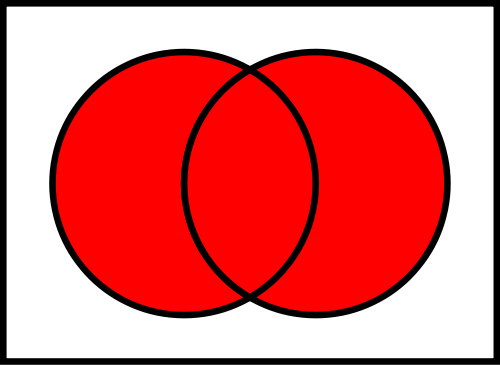
\includegraphics{AcupB}}
	\caption{Union}
	\end{subfigure}
&
	\begin{subfigure}{.25\textwidth}
	\resizebox{\linewidth}{!}{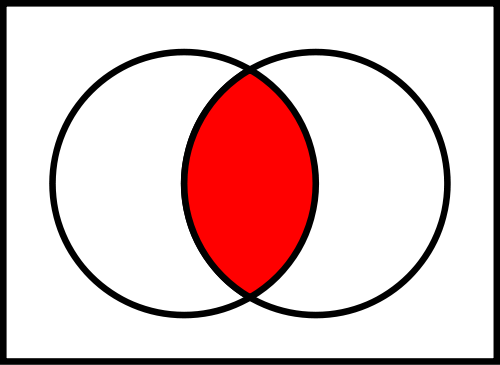
\includegraphics{AcapB}}
	\caption{Intersection}
	\end{subfigure}
&
	\begin{subfigure}{.25\textwidth}
	\resizebox{\linewidth}{!}{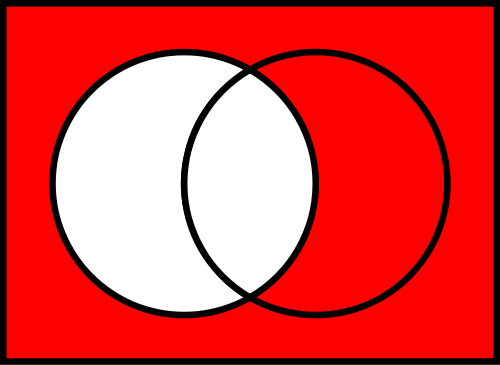
\includegraphics{Acomp}}
	\caption{Complement}
	\end{subfigure}
\end{tabular}
\end{figure}

\begin{center}
\begin{tabular}{|c|c||c|c|c|} \hline
Set Theory 		& 			& Logic			&		& \\ \hline
Union			& $A\cup B$	& Disjunction 	& OR 	& $\lor$	\\
Intersection		& $A\cap B$	& Conjunction	& AND 	& $\land$\\
Complement		& $A^c$		& Negation		& NOT 	& $\lnot$	\\ \hline
\end{tabular}
\end{center}

\break % <<

%----------------------------------------------------------------------
\subsection{Set algebra}
%----------------------------------------------------------------------
\begin{definition}
\ben
\it Commutative property.
\bit 
\it $A\cup B = B\cup A$,
\it $A\cap B = B\cap A$.
\eit
\it Associative property.
\bit 
\it $(A\cup B)\cup C = A\cup (B\cup C)$,
\it $(A\cap B)\cap C = A\cap (B\cap C)$.
\eit
\it Distributive property.
\bit 
\it $A\cup (B\cap C) = (A\cup B)\cap(A\cup C)$,
\it $A\cap (B\cup C) = (A\cap B)\cup(A\cap C)$.
\eit
\een
\end{definition}

\begin{remark}
A statement such as $A\cup B\cap C$ is ambiguous. 
\end{remark}

%----------------------------------------------------------------------
\section{De Morgan's laws}
%----------------------------------------------------------------------
Union and intersection swap roles under complementation.

\begin{theorem}\label{thm:demorgan_simple}
\ben
\it $(A\cup B)^c = A^c\cap B^c$.
\it $(A\cap B)^c = A^c\cup B^c$.
\een
\end{theorem}

\begin{proof}
\begin{enumerate}
\item % part (1)
Let $a\in(A\cup B)^c$. Then $a\notin A$ and $a\notin B$, so $a\in A^c\cap B^c$.
Hence $(A\cup B)^c\subseteq A^c\cap B^c$.\par
Let $a\in A^c\cap B^c$. Then $a\notin A$ and $a\notin B$, so $a\notin A\cup B$.
Hence $A^c\cap B^c\subseteq (A\cup B)^c$.\par
Thus it follows that $(A\cup B)^c = A^c\cap B^c$.
\item % part (2)
Apply part (1) to the sets $A^c$ and $B^c$: $(A^c\cup B^c)^c = A\cap B$.\par
Then take the complement of both sides: $(A\cap B)^c = A^c\cup B^c$.
\end{enumerate}
\end{proof}

%----------------------------------------------------------------------
\section{Set difference}
%----------------------------------------------------------------------
\begin{definition}
Let $A$, $B$ and $\Omega$ be sets, with $A,B\subseteq \Omega$.
\ben
\it The \emph{set difference} between $A$ and $B$ is the set
$$
A\setminus B = \{a\in \Omega : a\in A \text{ and } a\notin B\}. % = A\cap B^c.
$$
\it The \emph{symmetric difference} between $A$ and $B$ is the set 
$$
A\bigtriangleup B = (A\setminus B) \cup (B\setminus A). %= (A\cap B^c)\cup (B\cap A^c). 
$$
\een
\end{definition}

\bit
\it $A\setminus B$ is the set of points that are in $A$ but not in $B$.
\it $A\bigtriangleup B$ is the set of points that are in either $A$ or $B$, but not both.
\eit

% example
\begin{example}
Let $A=\{a,b\}$ and $B=\{b,c\}$. Then
\bit
\it $A\setminus B = \{a\}$
\it $A\bigtriangleup B = \{a,c\}$.
\eit
\end{example}

\break % <<


%----------------------------------------------------------------------
%\section*{Appendix: Set operations}
%----------------------------------------------------------------------
% figure
\begin{figure}[htb]
\centering

\begin{tabular}{cccc}	
\begin{subfigure}{.15\textwidth}
\resizebox{\linewidth}{!}{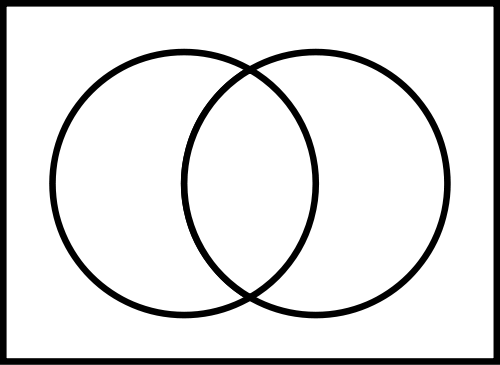
\includegraphics{emptyset}}
\caption{$\emptyset$}
\end{subfigure}
&
\begin{subfigure}{.15\textwidth}
\resizebox{\linewidth}{!}{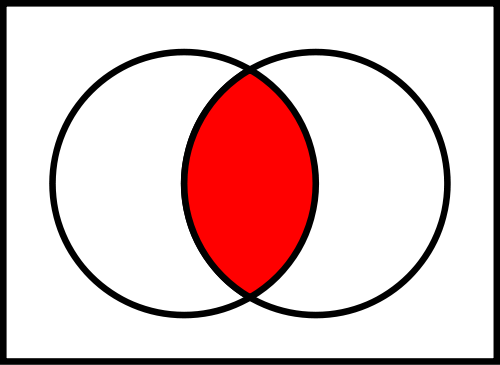
\includegraphics{AcapB}}
\caption{$A\cap B$}
\end{subfigure}
&
\begin{subfigure}{.15\textwidth}
\resizebox{\linewidth}{!}{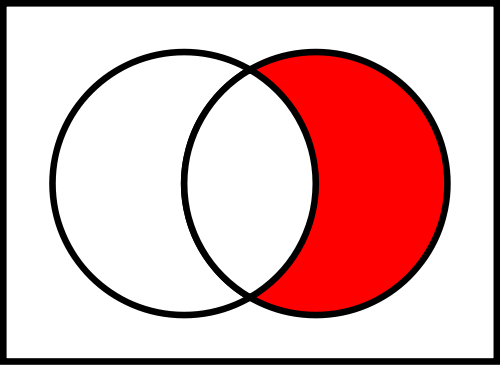
\includegraphics{BminusA}}
\caption{$B\setminus A$}
\end{subfigure}
&
\begin{subfigure}{.15\textwidth}
\resizebox{\linewidth}{!}{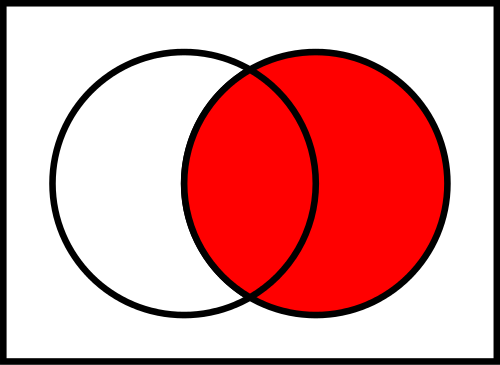
\includegraphics{setB}}
\caption{$B$}
\end{subfigure}
\end{tabular}

\begin{tabular}{cccc}
\begin{subfigure}{.15\textwidth}
\resizebox{\linewidth}{!}{
\includegraphics{AcupB_comp}}
\caption{$(A\cup B)^c$}
\end{subfigure}
&
\begin{subfigure}{.15\textwidth}
\resizebox{\linewidth}{!}{
\includegraphics{symdiff_comp}}
\caption{$(A\bigtriangleup B)^c$}
\end{subfigure}
&
\begin{subfigure}{.15\textwidth}
\resizebox{\linewidth}{!}{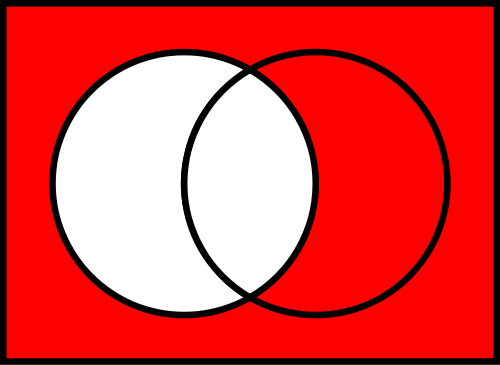
\includegraphics{Acomp}}
\caption{$A^c$}
\end{subfigure}
&
\begin{subfigure}{.15\textwidth}
\resizebox{\linewidth}{!}{
\includegraphics{AminusB_comp}}
\caption{$(A\setminus B)^c$}
\end{subfigure}
\end{tabular}

\begin{tabular}{cccc}
\begin{subfigure}{.15\textwidth}
\resizebox{\linewidth}{!}{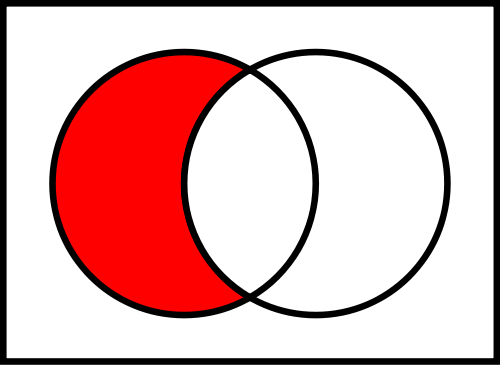
\includegraphics{AminusB}}
\caption{$A\setminus B$}
\end{subfigure}
&
\begin{subfigure}{.15\textwidth}
\resizebox{\linewidth}{!}{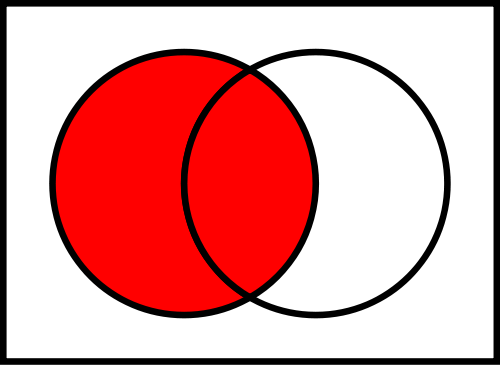
\includegraphics{setA}}
\caption{$A$}
\end{subfigure}
&
\begin{subfigure}{.15\textwidth}
\resizebox{\linewidth}{!}{
\includegraphics{symdiff}}
\caption{$A\bigtriangleup B$}
\end{subfigure}
&
\begin{subfigure}{.15\textwidth}
\resizebox{\linewidth}{!}{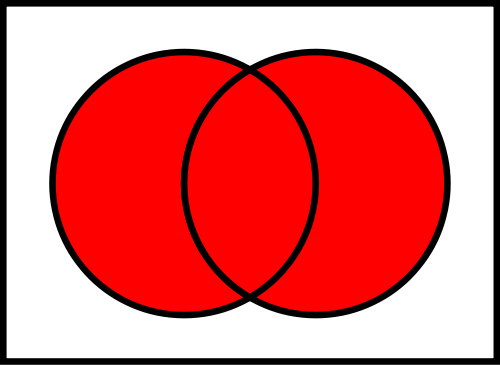
\includegraphics{AcupB}}
\caption{$A\cup B$}
\end{subfigure}
\end{tabular}

\begin{tabular}{cccc}
\begin{subfigure}{.15\textwidth}
\resizebox{\linewidth}{!}{
\includegraphics{Bcomp}}
\caption{$B^c$}
\end{subfigure}
&
\begin{subfigure}{.15\textwidth}
\resizebox{\linewidth}{!}{
\includegraphics{BminusA_comp}}
\caption{$(B\setminus A)^c$}
\end{subfigure}
&
\begin{subfigure}{.15\textwidth}
\resizebox{\linewidth}{!}{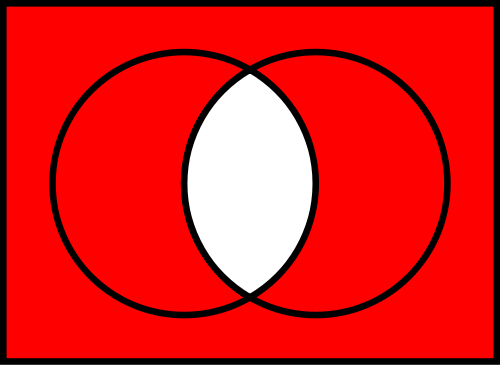
\includegraphics{AcapB_comp}}
\caption{$(A\cap B)^c$}
\end{subfigure}
&
\begin{subfigure}{.15\textwidth}
\resizebox{\linewidth}{!}{
\includegraphics{universe}}
\caption{$\emptyset^c$}
\end{subfigure}
\end{tabular}
\caption{Set Operations ($A$ on the left, $B$ on the right).\label{fig:set-operations}}
\end{figure}

%----------------------------------------------------------------------
\section{Exercises}
% !TEX root = main.tex

\begin{exercise}
\begin{questions}
\question
Illustrate the basic set operations using Venn diagrams.%, as shown in Figure~\ref{fig:set-operations}.
\question
State and prove De Morgan's laws.
\end{questions}
\end{exercise}

%======================================================================
\endinput
%======================================================================

%----------------------------------------------------------------------
%======================================================================
\endinput
%======================================================================

% !TEX root = main.tex
%======================================================================
\chapter{Events}\label{chap:events}
%======================================================================

\section*{A brief history of probability}
Games of chance have been played since antiquity, but the mathematical principles of chance and uncertainty were first established only in the 17th century.

\vspace*{4ex}
\begin{tabular}{lll}
1654		& Classical principles 	& Blaise Pascal (1623--1662) \\
    		&						& Pierre de Fermat (1601--1665)  \\
1657		& \textit{De Ratiociniis in Ludo Aleae} & Christiaan Huygens (1629--1695) \\
1713		& \textit{Ars Conjectandi} & Jakob Bernoulli (1654--1705) \\ 
1718		& \textit{The Doctrine of Chances} & Abraham de Moivre (1667--1754) \\
1812		& \textit{Theorie Analytique des Probabilites} & Pierre de Laplace (1749-1827) \\
1919		& Relative frequency & Richard von Mises (1883--1953) \\
1933		& Modern axiomatic theory & Andrey Kolmogorov (1903--1987)\\
\end{tabular}

%----------------------------------------------------------------------
\section{Sample spaces}
%----------------------------------------------------------------------
% defn: random_experiment/outcome/sample_space
\begin{definition}
\ben
\it
Any process of observation or measurement will be called an \emph{experiment} or \emph{trial}.
\it
Any experiment whose outcome is uncertain is called a \emph{random experiment}.
\it
A random experiment has a set of possible \emph{outcomes}.
\it
Each time a random experiment is performed, \emph{exactly one} of its outcomes will occur.
\it
The set of all possible outcomes is called the \emph{sample space} of the experiment, denoted by $\Omega$.
\it
Outcomes are also called \emph{elementary events}, and denoted by $\omega\in\Omega$.
\een
\end{definition}

\break

% example: sample spaces
\begin{example}
For any random experiment, the sample space is the set of all possible outcomes:
\begin{tabbing}
\underline{Experiment}\hspace{50ex} \= \underline{Sample space} \\[1ex]
A coin is tossed once.	\> $\Omega = \{H,T\}$ \\
A six-sided die is rolled once.	\> $\Omega=\{1,2,3,4,5,6\}$ \\
A coin is tossed repeatedly until a head occurs. \> $\Omega = \{1,2,3,\ldots\}$ \\
The height of a randomly chosen student is measured: \> $\Omega = [0,\infty)$
\end{tabbing}
\end{example}

%----------------------------------------------------------------------
\section{Events}
%----------------------------------------------------------------------

% defn: events
\begin{definition}
\bit
\it An \emph{event} $A$ is a subset of the sample space, $\Omega$. 
\it If outcome $\omega$ occurs, we say that event $A$ \emph{occurs} if and only if $\omega\in A$.
\it Two events $A$ and $B$ with $A\cap B=\emptyset$ are called \emph{disjoint} or \emph{mutually exclusive}.
\it The empty set $\emptyset$ is called the \emph{impossible event}.
\it The sample space $\Omega$ is called the \emph{certain event}.
\eit
\end{definition}

\begin{remark}
\bit
\it If $A$ occurs and $A\subseteq B$, then $B$ must also occur.
\it If $A$ occurs and $A\cap B=\emptyset$, then $B$ does not occur. 
\eit
\end{remark}

\break

% example: die
\begin{example}
A die is rolled once. The sample space can be represented by $\Omega=\{1,2,3,4,5,6\}$.\par
We may be interested in whether or not the following events occur:
\begin{tabbing}
\underline{Event}\qquad\qquad\qquad\qquad\qquad\qquad\qquad\qquad\qquad\qquad\qquad\qquad\=\underline{Subset} \\ 
The outcome is the number $1$.	\> $A = \{1\}$ \\
The outcome is an even number.	\> $A = \{2,4,6\}$ \\
The outcome is even but does not exceed $3$.	\> $A = \{2,4,6\}\cap\{1,2,3\}$ \\
The outcome is not even			\> $A = \Omega\setminus\{2,4,6\}$
\end{tabbing}
\end{example}

%----------------------------------------------------------------------
\section{Families of events}
%----------------------------------------------------------------------
\begin{definition}
Let $\Omega$ be any set. 
\ben
\it The set of all subsets of $\Omega$ is called its \emph{power set}, which we denote by $\mathcal{P}(\Omega)$.
\it Any subset of $\mathcal{P}(\Omega)$ is called a \emph{family of sets over $\Omega$}.
\een
\end{definition}

Let $\Omega$ be the sample space of some random experiment. 
If we are interested in events $A$ and $B$, we must also be interested in whether:

\begin{itemize}
\item event $A$ occurs \emph{or} event $B$ occurs -- this is the event $A\cup B$,
\item event $A$ occurs \emph{and} event $B$ occurs -- this is the event $A\cap B$,
\item event $A$ does \emph{not} occur -- this is the event $A^c$.
\end{itemize}

\smallskip
We cannot therefore use arbitrary families of sets over $\Omega$ as the basis for investigating random experiments. Instead, we allow only families that are \emph{closed} under certain set operations.

\break

\begin{definition}
A family of sets $\mathcal{F}$ over $\Omega$ is said to be
\ben
\it \emph{closed under complementation} if $A^c\in\mathcal{F}$ for every $A\in\mathcal{F}$, 
\it \emph{closed under pairwise unions} if $A\cup B\in\mathcal{F}$ for every $A,B\in\mathcal{F}$, 
\it \emph{closed under finite unions}	if $\bigcup_{i=1}^{n} A_i\in\mathcal{F}$ for every $A_1,A_2,\ldots A_n\in\mathcal{F}$,
\een
\end{definition}

% defn: fields of sets
\begin{definition}
A family of sets $\mathcal{F}$ over $\Omega$ is called a \emph{field of sets} over $\Omega$ if
\begin{enumerate}
\item $\Omega\in\mathcal{F}$,
\item $\mathcal{F}$ is closed under complementation, and
\item $\mathcal{F}$ is closed under pairwise unions.
\end{enumerate}
\end{definition}

\break

% example
\begin{example}\label{ex:fields_of_sets}
A six-sided die is rolled once, and the score is observed. A suitable sample space for this experiment is the set 
$\Omega=\{1,2,3,4,5,6\}$. The power set of $\Omega$ will always provide a field of sets to work with. However, suppose we are only interested in whether or not the outcome is an even number. In this case, we need only consider the following family of events:
\[
\mathcal{F} = \big\{\emptyset, \{1,3,5\}, \{2,4,6\}, \{1,2,3,4,5,6\}\big\}.
\]
We can see that $\mathcal{F}$ is a field of sets over $\Omega$, because
\ben
\it it contains the sample space $\{1,2,3,4,5,6\}$,
\it the complement of every set in $\mathcal{F}$ is also contained in $\mathcal{F}$, and
\it the union of any two sets in $\mathcal{F}$ is also contained in $\mathcal{F}$.
\een
\end{example}

\break

% properties of fields
\begin{theorem}[Properties of fields]
Let $\mathcal{F}$ be a field over $\Omega$. Then
\begin{enumerate}
\item $\emptyset\in\mathcal{F}$,
\item $\mathcal{F}$ is closed under pairwise intersections,
\item $\mathcal{F}$ is closed under set differences.
\end{enumerate}
\end{theorem}

\begin{proof}
\begin{enumerate}
\item
We know that $\emptyset = \Omega^c$, and that $\Omega\in\mathcal{F}$. Because $\mathcal{F}$ is closed under complementation, it thus follows that $\emptyset\in\mathcal{F}$.
\item
Let $A,B\in\mathcal{F}$. By De Morgan's laws, we have that $A\cap B = (A^c\cup B^c)^c$. Because $\mathcal{F}$ is closed under complementation and pairwise unions, it thus follows that $A\cap B\in\mathcal{F}$.
\item
Let $A,B\in\mathcal{F}$. Set difference can be written as $A\setminus B = A\cap B^c$. Furthermore, by De Morgan's laws we see that $A\cap B^c = (A^c\cup B)^c$. Because $\mathcal{F}$ is closed under complementation and pairwise unions, it thus follows that $A\setminus B\in\mathcal{F}$.
\end{enumerate}
\end{proof}

%----------------------------------------------------------------------
\section{Terminology}
%----------------------------------------------------------------------
\begin{table}[h]
\centering\small
\begin{tabular}{|c|l|l|} \hline
Notation 			& Set theory			& Probability theory \\ \hline
$\Omega$			& Universal set			& Sample space \\ 
$\omega\in\Omega$	& Element of $\Omega$	& Elementary event, outcome \\
$A\subseteq\Omega$	& Subset of $\Omega$	& Event $A$ \\
$A\subseteq B$		& Inclusion				& If $A$ occurs, then $B$ occurs \\
$A\cup B$			& Union					& $A$ or $B$ occurs \\ 
$A\cap B$			& Intersection			& $A$ and $B$ occur\\ 
$A^c$				& Complement of $A$		& $A$ does not occur \\
$A\setminus B$		& Difference			& $A$ occurs, but $B$ does not \\
$A\bigtriangleup B$	& Symmetric difference	& $A$ or $B$ occurs, but not both \\
$\emptyset$			& Empty set 			& Impossible event \\
$\Omega$			& Universal set			& Certain event \\ \hline
\end{tabular}
%\caption*{Table of correspondence (Grimmett \& Stirzaker 2001).}
\end{table}


%----------------------------------------------------------------------
\section{Exercises}
% !TEX root = main.tex

\begin{exercise}
\begin{questions}
%----------------------------------------
% events
\question
Identify a sample space, and the subset corresponding to event $A$, in each of the following scenarios:
\begin{parts}
%--------------------
\part A coin is tossed three times. $A$ is the event that at least two heads are obtained.
\begin{answer}
\par
$\Omega	= \{HHH, HHT, HTH, THH, HTT, THT, TTH, TTT\}$ and $A = \{HHH, HHT, HTH, THH\}$. Alternatively, if we are only interested in the number of heads, we could take $\Omega=\{0,1,2,3\}$ and $A=\{2,3\}$.
\end{answer}
%--------------------
\part A game of football is played. $A$ is the event that the match ends in a draw.
\begin{answer}
$\Omega=\{(a,b):a,b = 0,1,2,\ldots\}$ and $A=\{(a,b): a=b\}$ where $a$ and $b$ are the numbers of goals scored by the first and second teams, respectively. Note that this is a (countably) infinite set. 
\par
Alternatively, we could take $\Omega=\{W,D,L\}$ and $A=\{D\}$ where $W,D,L$ are respectively the events that the first team wins, draws or loses the game.
\end{answer}
%--------------------
\part A couple have two children. $A$ is the event that both are girls.
\begin{answer}
$\Omega=\{GG,GB,BG,BB\}$ and $A=\{GG\}$.
\par
Alternatively, we could take $\Omega=\{0,1,2\}$ and $A=\{2\}$.
\end{answer}
%--------------------
\part A shot hits a circular target of radius 10cm. $A$ is the event that the shot hits within 3cm of the centre.
\begin{answer}
$\Omega=\{(x,y): x^2+y^2\leq 10^2\}$ and $A=\{(x,y): x^2+y^2\leq 3^2\}$.
\end{answer}
\end{parts}

%----------------------------------------
% properties of fields
\question
A family of sets $\mathcal{F}$ over $\Omega$ is said to be
\bit
\it \emph{closed under finite unions} if $A_1\cup A_2\cup\ldots\cup A_n\in\mathcal{F}$ whenever $A_1,A_2,\ldots A_n\in\mathcal{F}$,
\it \emph{closed under finite intersections} if $A_1\cap A_2\cap\ldots\cap A_n\in\mathcal{F}$ whenever $A_1,A_2,\ldots A_n\in\mathcal{F}$.
\eit
Suppose that $\mathcal{F}$ is a field of sets over $\Omega$. Show that
\begin{parts}
%--------------------
%--------------------
\part $\mathcal{F}$ is closed under finite unions, and that
\begin{answer}
Proof by induction. Suppose that $\mathcal{F}$ is closed under unions of $n$ sets (where $n\geq 2$). Let $A_1,A_2,\ldots,A_{n+1}\in\mathcal{F}$. By the inductive hypothesis, $\cup_{i=1}^nA_i\in\mathcal{F}$. Thus $\cup_{i=1}^{n+1} A_i = \big[\cup_{i=1}^{n} A_i\big] \cup A_{n+1} \in\mathcal{F}$, because $\mathcal{F}$ is closed under pairwise unions.
\end{answer}
%--------------------
\part $\mathcal{F}$ is closed under finite intersections.
\begin{answer}
Let $A_1,A_2,\ldots,A_n\in\mathcal{F}$. Then $\cap_{i=1}^n A_i = \big[\cup_{i=1}^n A_i^c\big]^c$ (De Morgan's laws). Hence $\cap_{i=1}^n A_i\in\mathcal{F}$ because $\mathcal{F}$ is closed under complementation and finite unions. 
\end{answer}
%--------------------
\end{parts}
%----------------------------------------
\end{questions}
\end{exercise}

%======================================================================
\endinput
%======================================================================

%----------------------------------------------------------------------

%======================================================================
\endinput
%======================================================================

% !TEX root = main.tex
%======================================================================
\chapter{Probability}\label{chap:prob}
%======================================================================

%----------------------------------------------------------------------
\section{Probability measures}
%----------------------------------------------------------------------
Probability is defined to be a \emph{function} that assigns numerical value to random events.

\begin{definition}
Let $\Omega$ be the sample space of some random experiment, and let $\mathcal{F}$ be a field of sets over $\Omega$. A \emph{probability measure} on $(\Omega,\mathcal{F})$ is a function 
\[
\begin{array}{rccl}
	\prob:	& \mathcal{F}	& \to	& [0,1] \\[1ex]
			& A				& \mapsto	& \prob(A)
\end{array}
\]
such that $\prob(\Omega) = 1$, and for any countable collection of pairwise disjoint events $\{A_1,A_2,\ldots\}$,
\[
\prob\left(\bigcup_{i=1}^\infty A_i\right) = \sum_{i=1}^{\infty} \prob(A_i).
\]
The triple $(\Omega,\mathcal{F},\prob)$ is called a \emph{probability space}.
\end{definition}

\begin{remark}
\bit
\it The second property is called \emph{countable additivity}.
\it The number $\prob(A)$ is called the \emph{probability} of event $A\in\mathcal{F}$.
\eit
\end{remark}

\break

% example: die
\begin{example}
Consider a random experiment in which a fair six-sided die is rolled once.
\bit
\it A suitable sample space for the experiment is $\Omega=\{1,2,3,4,5,6\}$.
\it A suitable field of events for the experiment is the power set, $\mathcal{F} = \mathcal{P}(\Omega)$.
\it Because the die is fair, a suitable probability measure is given by the function
\[\begin{array}{rcl}
\prob:	\mathcal{F} & \to 		& [0,1] \\
		A			& \mapsto 	& \frac{1}{6}|A|, \qquad\text{where $|A|$ denotes the cardinality of $A$.}

\end{array}\] 
\eit

\begin{tabbing}
\underline{Event}\qquad\qquad\qquad\qquad\qquad\qquad\qquad\qquad\qquad
	\=\underline{Event}\qquad\qquad\qquad\qquad\qquad
	\=\underline{Probability} \\
The outcome is the number $1$.	\> $A = \{1\}$ \> $\prob(A) = 1/6$\\
The outcome is an even number.	\> $A = \{2,4,6\}$  \> $\prob(A) = 3/6$\\
The outcome is even but does not exceed $3$.	\> $A = \{2,4,6\}\cap\{1,2,3\}$  \> $\prob(A) = 1/6$\\
The outcome is not even			\> $A = \Omega\setminus\{2,4,6\}$ \> $\prob(A) = 3/6$
\end{tabbing}
\end{example}

\newpage
\break
% example
\begin{example}
A fair six-sided die is rolled once. If we are only interested in whether the outcome is an odd or even number, we can take
\bit
\it Sample space: $\Omega=\{1,2,3,4,5,6\}$,
\it Events: $\mathcal{F} = \big\{\emptyset,\{1,3,5\},\{2,4,6\},\{1,2,3,4,5,6\}\big\}$
\it Probability measure: $\prob(\emptyset)=0$, $\prob(\{1,3,5\})=1/2$, $\prob(\{2,4,6\})=1/2$, $\prob(\{1,2,3,4,5,6\})=1$.
\eit
\end{example}

%----------------------------------------------------------------------
\section{Properties of probability measures}
%----------------------------------------------------------------------

% theorem: properties of probability measures
\begin{theorem}[Properties of probability measures]\label{thm:properties_of_probability_measures}
Let $(\Omega,\mathcal{F},\prob)$ be a probability space, and let $A,B\in\mathcal{F}$. 
\ben
\it Complementarity: $\prob(A^c) = 1 - \prob(A)$.
\it $\prob(\emptyset) = 0$,
\it Monotonicity: if $A\subseteq B$ then $\prob(A)\leq \prob(B)$.
\it Addition rule: $\prob(A\cup B) = \prob(A) + \prob(B) - \prob(A\cap B)$.
\een
\end{theorem}

\break

% proof
\begin{proof}
\ben
\it % complementarity
Since $A\cup A^c=\Omega$ is a disjoint union and $\prob(\Omega)=1$, it follows by additivity that 
\[
1 = \prob(\Omega) = \prob(A\cup A^c) = \prob(A) + \prob(A^c).
\]
\it % emptyset
Since $\emptyset=\Omega^c$ and $\prob(\Omega)=1$, it follows by complemenarity that
\[
\prob(\emptyset) = \prob(\Omega^c) = 1 - \prob(\Omega) = 1 - 1 = 0.
\]
\it % monotonicity
Let $A\subseteq B$ and let us write $B = A\cup (B\setminus A)$. 

Since $A$ and $B\setminus A$ are disjoint sets, it follows by additivity that
\[
\prob(B) = \prob\big[A\cup (B\setminus A)\big] = \prob(A) + \prob(B\setminus A).
\]
Hence, because $\prob(B\setminus A)\geq 0$, it follows that $\prob(B) \geq \prob(A)$.

\break

\it % addition rule
Let us write:
\bit
\it $A\cup B = (A\setminus B) \cup (B\setminus A) \cup (A\cap B)$
\it $A 		 = (A\setminus B) + (A\cap B)$
\it $B 		 = (B\setminus A) + (A\cap B)$
\eit
These are disjoint unions, so by additivity, 
\bit
\it $\prob(A\cup B) = \prob(A\setminus B) + \prob(B\setminus A) + \prob(A\cap B)$
\it $\prob(A) 		= \prob(A\setminus B) + \prob(A\cap B)$
\it $\prob(B)		= \prob(B\setminus A) + \prob(A\cap B)$
\eit
Hence $\prob(A\cup B) = \prob(A) + \prob(B) - \prob(A\cap B)$, as required.
\een
\end{proof}


%----------------------------------------------------------------------
\section{Exercises}
% !TEX root = main.tex

\begin{exercise}
\begin{questions}
%----------------------------------------
% bookwork
\question
What does it mean to say that $\prob$ is a probability measure over $(\Omega,\mathcal{F})$?
\begin{answer}
Bookwork. The symbols $\Omega$ (sample space) and $\mathcal{F}$ (field of events) should be defined before giving the definition of $\prob$.
\end{answer}
%--------------------
% subadditivity
\question
%Let $(\Omega,\mathcal{F},\prob)$ be a probability space. 
Show that $\prob(A\cup B) \leq \prob(A)+\prob(B)$ for any two events $A$ and $B$.
\begin{answer}
First we express $A$, $B$ and $A\cup B$ as disjoint unions: 
\begin{align*}
A		& = (A\cap B^c)\cup (A\cap B) \\ 
B		& = (B\cap A^c)\cup (A\cap B) \\ 
A\cup B	& = (A\cap B^c)\cup (A\cap B) \cup (B\cap A^c)
\end{align*}
By the additivity property of probability measures,
\begin{align*}
\prob(A) 		& = \prob(A\cap B^c) + \prob(A\cap B) \\
\prob(B) 		& = \prob(B\cap A^c) + \prob(A\cap B) \\
\prob(A\cup B) 	& = \prob(A\cap B^c) + \prob(A\cap B) + \prob(B\cap A^c) \\
\end{align*}
From here, it follows that $\prob(A\cup B)=\prob(A)+\prob(B)-\prob(A\cap B)$, and because $\prob(A\cap B)\geq 0$ for any two events $A,B\mathcal{F}$, we see that $\prob(A\cup B) \leq \prob(A)+\prob(B)$, as required.
\end{answer}
%--------------------
% numerical
\question
Let $A$ and $B$ be events such that $\prob(A)=0.4$, $\prob(B)=0.5$ and $\prob(A~\cup~B)=0.8$.\par
Compute the following probabilities:
\begin{parts}
%----------
\part $\prob(A\cap B)$.
\begin{answer}
$\prob(A\cap B) = \prob(A) + \prob(B) - \prob(A\cup B) = 0.4 + 0.5 - 0.8 = 0.1$.
\end{answer}
%----------
\part $\prob(A\cup B^c)$.
\begin{answer}
$\prob(A\cup B^c) = 1 - \prob(B\setminus A) = 1 - \big[\prob(B)-\prob(A\cap B)\big] = 1 - 0.4 = 0.6$.
\end{answer}
\end{parts}
%----------------------------------------
% inequalities
\question
Let $A$ and $B$ be random events, with probabilities $\prob(A) = 1/2$ and $\prob(B) = 3/4$. 
\begin{parts}
%--------------------
\part Show that $\displaystyle\frac{1}{4}\leq \prob(A\cap B)\leq\frac{1}{2}$.
\begin{answer}
$A\cap B\subseteq A$ and $A\cap B\subseteq B$ means that:
\[
\prob(A\cap B) \leq \min\big\{\prob(A),\prob(B)\big\} = \displaystyle\frac{1}{2}.
\]
Furthermore, $\prob(A\cup B)\leq 1$ means that:
\[
\prob(A\cap B) = \prob(A)+\prob(B)-\prob(A\cup B) \geq \displaystyle\frac{1}{4}.
\]
\end{answer}
%--------------------
\part Show that $\displaystyle\frac{3}{4}\leq \prob(A\cup B)\leq 1$.
\begin{answer}
$A\subseteq A\cup B$ and $B\subseteq A\cup B$ means that:
\[
\prob(A\cup B) \geq \max\big[\prob(A),\prob(B)\big] = \displaystyle\frac{3}{4}.
\]
Furthermore, $\prob(A\cup B)\leq 1$ means that:
\[
\prob(A\cup B) \leq \min\{1,\prob(A)+\prob(B)\} = 1.
\]
\end{answer}
\end{parts}

%----------------------------------------
\end{questions}
\end{exercise}

%======================================================================
\endinput
%======================================================================

%----------------------------------------------------------------------

%======================================================================
\endinput
%======================================================================

% !TEX root = main.tex
%======================================================================
\chapter{Conditional Probability}\label{chap:conditional}
%======================================================================

%----------------------------------------------------------------------
\section{Conditional probability}
%----------------------------------------------------------------------

% modern
Let $(\Omega,\mathcal{F},\prob)$ be a probability space, and let $A,B\in\mathcal{F}$ be any two events.
\bit
\it If $B$ occurs and $A\cap B = \emptyset$, then $A$ cannot occur.
\it If $B$ occurs and $B\subseteq A$, then $A$ is certain to occur.
\it If $B$ occurs, then $A$ will also occur \emph{if and only if} the event $A\cap B$ occurs.
\eit

Given that $B$ occurs, the probability that $A$ also occurs is $\prob(A\cap B)$ expressed as a proportion of $\prob(B)$.

% definition
\begin{definition}
If $\prob(B)>0$, the \emph{conditional probability of $A$ given $B$} is defined to be
\[
\prob(A|B) = \frac{\prob(A\cap B)}{\prob(B)}
\]
\end{definition}

% remark
\begin{remark}
\bit
\it $\prob(A|B) = 0$ whenever $A\cap B = \emptyset$, and
\it $\prob(A|B) = 1$ whenever $B\subseteq A$.
\eit
\end{remark}

% example
\begin{example}
Let $A$ and $B$ be two events, with probabilities $\prob(A)=0.3$, $\prob(B)=0.8$ and $\prob(A\cap B)=0.2$.\par
Find the probabilities $\prob(A\cup B)$, $\prob(A\cap B^c)$, $\prob(A|B)$ and $\prob(A|B^c)$.
\begin{solution}
\ben
\it $\prob(A\cup B) = \prob(A) + \prob(B) - \prob(A\cap B) = 0.3 + 0.8 - 0.2 = 0.9$
\it $\prob(A\cap B^c) = \prob(A) - \prob(A\cap B) = 0.3 - 0.2 = 0.1$
\it $\prob(A|B)   = \prob(A\cap B)/\prob(B) = 0.2/0.8 = 0.25$
\it $\prob(A|B^c) = \prob(A\cap B^c))/\prob(B^c) = 0.1/0.2 = 0.5$
\een
\end{solution}
\end{example}

\begin{example}[The Second Child Paradox]
If we know that a man has two children, and that one of them is a boy, what is the probability that he has two boys?
\begin{solution}
%\bit
%\it Initially there are four equally-likely outcomes: $\Omega=\{BB, BG, GB, GG\}$.
%\it The statement rules out the last of these outcomes ($GG$).
%\it The remaining possibilities are $BB$, $BG$ and $GB$
%\it Hence the probability that the man has two boys is 1/3. 
%\eit
Let $\Omega=\{BB, BG, GB, GG\}$ denote the sample space, and let $A=\{BB, BG, GB\}$ be the event that the man has at least one boy. Then
\[
\prob(\{BB\}|A) = \frac{\prob(\{BB\}\cap A)}{\prob(A)} = \frac{\prob(\{BB\})}{\prob(\{BB,BG,GB\})} = \frac{1/4}{3/4} = \frac{1}{3}.
\]
\end{solution}
\end{example}


%----------------------------------------------------------------------
\section{The partition theorem}
%----------------------------------------------------------------------

% definition: partition
\begin{definition}
A \emph{partition} of a set $B$ is a collection of non-empty sets $\{A_1,A_2,\ldots\}$ such that every element of $B$ lies in exactly one of these sets, or equivalently,
\ben
\it $A_i\cap A_j = \emptyset$ for all $i\neq j$, and 
\it $B\subseteq\bigcup_{i=1}^{\infty} A_i$.
\een
\end{definition}

% theorem: law of total probability
\begin{theorem}[The Partition Theorem]\label{thm:partition}
If $\{A_1,A_2,\ldots\}$ is a partition of $B$, then
\[
\prob(B) = \sum_{i=1}^{\infty} \prob(B\cap A_i) = \sum_{i=1}^{\infty} \prob(B|A_i)\prob(A_i)
\]
\end{theorem}

% proof
\begin{proof}
First we write $B$ as a disjoint union
\[
B = (B\cap A_1)\cup (B\cap A_2)\cup \ldots = \bigcup_{i=1}^{\infty}(B\cap A_i)
\]
By the countable additivity of probability measures,
\begin{align*}
\prob(B)
	& = \prob\left(\bigcup_{i=1}^{\infty}(B\cap A_i)\right) \\
	& = \sum_{i=1}^{\infty}\prob(B\cap A_i) \\
	& = \sum_{i=1}^{\infty} \prob(B|A_i)\prob(A_i).
\end{align*}
\end{proof}

%----------------------------------------------------------------------
\section{Bayes' theorem}
%----------------------------------------------------------------------

\begin{lemma}\label{lem:bayes}
For any two events $A$ and $B$ such that $\prob(B)>0$,
\[
\prob(A|B) = \frac{\prob(B|A)\prob(A)}{\prob(B)}.
\]
\end{lemma}

\begin{proof}
Set intersection is a commutative operation, so
\[
\prob(A|B) = \frac{\prob(A\cap B)}{\prob(B)} = \frac{\prob(B\cap A)}{\prob(B)} = \frac{\prob(B|A)\prob(A)}{\prob(B)}.
\]
\end{proof}

% theorem: Bayes' theorem
\begin{theorem}[Bayes' Theorem]\label{thm:bayes}
Let $\{A_1,A_2,\ldots\}$ be a partition of an event $B$ and suppose that $\prob(B)>0$. Then
\[
\prob(A_i|B) = \frac{\prob(B|A_i)\prob(A_i)}{\sum_{j=1}^{\infty} \prob(B|A_j)\prob(A_j)}
\]
\end{theorem}

% proof
\begin{proof}
By Lemma~\ref{lem:bayes},
\[
\prob(A_i|B) 
	= \frac{\prob(B|A_i)\prob(A_i)}{\prob(B)}
	= \frac{\prob(B|A_i)\prob(A_i)}{\sum_{j=1}^{\infty} \prob(B|A_j)\prob(A_j)}
\]
where the last equality follows by the partition theorem.
\end{proof}

% example
\begin{example}
Bob tries to buy a newspaper every day. He tries in the morning with probability $1/3$, in the evening with probability $1/2$ and forgets completely with probability $1/6$. The probability of successfully buying a newspaper in the morning is $9/10$ (plenty of copies left), and in the evening is $2/10$ (often sold out). If Bob buys a newspaper, what is the probability that he bought it in the morning?
\end{example}

% solution
\begin{solution}
Let $M$ be the event that Bob tries to buy a newspaper in the morning, $E$ the event that he tries in the evening, and $F$ the event that he forgets completely. Then
\[
\prob(M) = 1/3, \qquad \prob(E) = 1/2, \qquad \prob(F) = 1/6.
\]
Let $N$ denote the event that Bob buys a newspaper. Then
\[
\prob(N|M) = 9/10, \qquad \prob(N|E) = 2/10, \qquad \prob(N|F) = 0.
\]
By Bayes' Theorem,
\begin{align*}
\prob(M|N) = \frac{\prob(N|M)\prob(M)}{\prob(N)}
	& = \frac{\prob(N|M)\prob(M)}{\prob(N|M)\prob(M) + \prob(N|E)\prob(E) + \prob(N|F)\prob(F)} \\
	& = \frac{9/10\times 1/3}{(9/10\times 1/3) + (2/10\times 1/2) + (0\times 1/6)} \\
	& = 3/4
\end{align*}
If Bob buys a newspaper, the probability that he bought it in the morning is $0.75$.
\end{solution}


%----------------------------------------------------------------------
\section{Exercises}
%----------------------------------------------------------------------

%----------------------------------------
\begin{exercise}
\begin{questions}
%----------------------------------------

% conditional prob
\question
Let $A$ and $B$ be events such that $\prob(A)=0.4$, $\prob(B)=0.5$ and $\prob(A\cup B)=0.8$.
Compute the following probabilities:
\begin{parts}
\part $\prob(A\cap B)$
\begin{answer}
$\prob(A\cap B) = \prob(A) + \prob(B) - \prob(A\cup B) = 0.4 + 0.5 - 0.8 = 0.1$.
\end{answer}
\part $\prob(A\cup B^c)$
\begin{answer}
$\prob(A\cup B^c) = 1 - \prob(B\setminus A) = 1 - \big[\prob(B)-\prob(A\cap B)\big] = 1 - 0.4 = 0.6$.
\end{answer}
\part $\prob(A\,|\,B)$
\begin{answer}
$\prob(A|B) = \prob(A\cap B)/\prob(B) = 0.1/0.5 = 0.2$.
\end{answer}
\part $\prob(A\,|\,A\cup B)$
\begin{answer}
$\prob(A|A\cup B) 	= \prob(A)/\prob(A\cup B) = 0.4/0.8 = 0.5$.
\end{answer}
\end{parts}

%----------------------------------------
% cond
\question
A student has three opportunities to pass an exam. The probability of failing the first attempt is 0.6; the probability of failing the second attempt, given that they have failed the first is 0.75, and the probability of failing the third attempt, given that they have failed the first and second is 0.4.
\begin{parts}
\part What is the probability that the student eventually passes the exam.
\begin{answer}
Let $F_i$ denote the event that the student fails at the $i$th
attempt, so that 
\[
\prob(F_1)=0.6,\quad \prob(F_2|F_1)=0.75\quad\mbox{and}\quad \prob(F_3|F_1\cap F_2)=0.4
\]
The probability that the student fails all three attempts is
\[
\prob(F_1\cap F_2\cap F_3) = \prob(F_1)\prob(F_2|F_1)\prob(F_3|F_1\cap F_2) = 0.6\times 0.75\times 0.4 = 0.18
\]
Hence, the probability that the student eventually passes is $1 - 0.18 = 0.82$.
%\paragraph{The chain rule:} The probability that events $A$ and $B$ both occur is $\prob(A\cap B) = \prob(B|A)\prob(A)$: this is sometimes called the \emph{chain rule}. For three events $A$, $B$ and $C$, the probability that all three occur is
%\begin{align*}
%\prob(A\cap B\cap C)
%	& = \prob\big((A\cap B)\cap C\big) \\
%	& = \prob(C|A\cap B)\prob(A\cap B) \\
%	& = \prob(C|A\cap B)\prob(B|A)\prob(A) \\
%\end{align*}
%Similarly, the probability that $A$, $B$, $C$ and $D$ all occur is
%\begin{align*}
%\prob(A\cap B\cap C\cap D) 
%	& = \prob\big((A\cap B\cap C)\cap D\big)	\\
%	& = \prob(D|A\cap B\cap C)\prob(A\cap B\cap C) \\
%	& = \prob(D|A\cap B\cap C)\prob(C|A\cap B)\prob(B|A)\prob(A) \\
%\end{align*}
%and so on.
\end{answer}
\part What are the respective probabilities of passing at the first, second and third attempts.
\begin{answer}
The probability that the student passes on the first attempt is $1-\prob(F_1) = 1-0.6 = 0.4$.
\par
The probability that the student takes a second test is $\prob(F_1)=0.6$. If the second test is taken, the (conditional) probability that the student passes it is $1-\prob(F_2|F_1) = 1-0.75 =
0.25$. Hence, the probability that the student passes on the second attempt is $0.6\times 0.25 = 0.15$.
\par
Similarly, the probability that the student takes the third test is $\prob(F_1\cap F_2) = \prob(F_1)\prob(F_2|F_1) = 0.6\times 0.75 = 0.45$. If the third test is taken, the (conditional) probability that the student passes it is $1-\prob(F_3|F_1\cap F_2)= 1-0.4 = 0.6$. Hence, the probability that the student passes on the third attempt is $0.45\times 0.6 = 0.27$. (The probability of eventually passing is $0.4 + 0.15 + 0.27 = 0.82$, which agrees with the answer to part (a).)
\end{answer}
\end{parts}

%----------------------------------------
\end{questions}
\end{exercise}
%----------------------------------------

%----------------------------------------------------------------------
\section{Assessment}
%----------------------------------------------------------------------

%----------------------------------------
\begin{exercise}
\begin{questions}
%----------------------------------------
% conditional prob
\question
Let $A$, $B$ and $C$ be events such that $\prob(A)=0.7$, $\prob(B)=0.6$, $\prob(C)=0.5$, $\prob(A\cap B)=0.4$, $\prob(A\cap C)=0.3$, $\prob(B\cap C)=0.2$ and $\prob(A\cap B\cap C)=0.1$.
Compute the following probabilities:
\begin{parts}
%--------------------
\part $\prob(A\cup B)$
\begin{answer}
$\prob(A\cup B) 
	= \prob(A) + \prob(B) - \prob(A\cap B) 
	= 0.7 + 0.6 - 0.4 
	= 0.9$.
\end{answer}
%----------
\part $\prob(A|B)$
\begin{answer}
$\displaystyle\prob(A|B) 
	= \frac{\prob(A\cap B)}{\prob(B)} 
	= \frac{0.4}{0.6} 
	= \frac{2}{3}$.
\end{answer}
%----------
\part $\prob(A\,|\,A\cup B)$
\begin{answer}
$\prob(A|A\cup B) 
	= \displaystyle\frac{\prob[A\cap (A\cup B)]}{\prob(A\cup B)} 
	= \displaystyle\frac{\prob(A)}{\prob(A\cup B)} 
	= \frac{0.7}{0.9} 
	= \frac{7}{9}$.
\end{answer}
%--------------------
\part $\prob(A\cup B\cup C)$
\begin{answer}
By the inclusion-exclusion principle,
\begin{align*}
\prob(A\cup B\cup C)
	& = [\prob(A) + \prob(B) + \prob(C)] - [\prob(A\cap B) + \prob(A\cap C) + \prob(B\cap C)] + \prob(A\cap B\cap C) \\
	& = (0.7 + 0.6 + 0.5) - (0.4 + 0.3 + 0.2) + 0.1 = 1.
\end{align*}
\end{answer}
%----------
\part $\prob(A^{c}\cap B^{c}\cap C)$
\begin{answer}
Because $A^{c}\cap B^{c}\cap C = (A\cup B)^{c}\cap C$, the sets $A\cup B$ and $A^{c}\cap B^{c}\cap C$ form a partition of $A\cup B\cup C$. Hence $\prob(A^{c}\cap B^{c}\cap C) = \prob(A\cup B\cup C) - \prob(A\cup B) = 1.0 - 0.9 = 0.1$
\end{answer}
%----------
\part $\prob(A^{c}\cap B^{c}\cap C|A\cup B)$.
\begin{answer}
Because $A^{c}$ and $A$ are disjoint, $\prob(A^{c}\cap B^{c}\cap C|A\cup B) = 0$.
\end{answer}
\end{parts}

%----------------------------------------
% bayes (insurance company)
\question
An insurance company divides its customers into three categories: $60$\% of customers are classed as low-risk, $30$\% as moderate-risk and $10$\% as high-risk. The probabilities that low-risk customers, moderate-risk customers and high-risk customers make a claim in any given year are $0.01$, $0.1$ and $0.5$ respectively. Given that a customer makes a claim this year, what is the probability that the customer is in the high-risk category?

\begin{answer}
Let $L$ denote the event that the customer is low-risk, $M$ the event that the customer is moderate-risk, and $H$ the event that the customer is high-risk:
\[
\prob(L) = 0.6,\quad \prob(M) = 0.3,\quad \prob(H) = 0.1.
\]
Let $C$ be the event that the customer makes a claim this year:
\[
\prob(C\,|\,L) = 0.01,\quad \prob(C\,|\,M) = 0.1,\quad \prob(C\,|\,H) = 0.5.
\]
We need to find $\prob(H\,|\,C)$:
\[
\prob(H\,|\,C) = \frac{\prob(H\cap C)}{\prob(C)} = \frac{\prob(C\,|\,H)\prob(H)}{\prob(C)}.
\]
The events $\{L,M,H\}$ form a partition of sample space (the set of all customers), so by the law of total probability,
\[
\prob(C) = \prob(C\,|\,L)\prob(L) + \prob(C\,|\,M)\prob(M) + \prob(C\,|\,H)\prob(H),
\]
and hence
\[
\prob(H\,|\,C) = \frac{\prob(C\,|\,H)\prob(H)}{\prob(C\,|\,L)\prob(L) + \prob(C\,|\,M)\prob(M) + \prob(C\,|\,H)\prob(H)},
\]
which is Bayes' theorem. The probability that a customer is in the high-risk category, given that the customer makes a claim this year, is 
\[
\prob(H\,|\,C) 
	= \frac{(0.5\times 0.1)}{(0.01\times 0.6) + (0.1\times 0.3) + (0.5\times 0.1)}
	= 0.5814\quad\text{(approx.).}
\]
\end{answer}


%----------------------------------------
\end{questions}
\end{exercise}
%----------------------------------------

%======================================================================
\endinput
%======================================================================

% !TEX root = main.tex
%======================================================================
\chapter{Independence}\label{chap:independence}
%======================================================================

%----------------------------------------------------------------------
\section{Independence}
%----------------------------------------------------------------------
If the probability that event $A$ occurs is \emph{not} affected by whether or not event $B$ occurs, then
$
\prob(A|B) = \prob(A).
$
In such cases, we say that events $A$ and $B$ are \emph{independent}:

% definition: independence
\begin{definition}
Two events $A$ and $B$ are said to be \emph{independent} if $\prob(A\cap B) = \prob(A)\prob(B)$.
\end{definition}

% lemma
\begin{lemma}
If $A$ and $B$ are independent, then $A$ and $B^c$ are also independent.
\end{lemma}
% proof
\begin{proof}
\[\begin{array}{ll}
\prob(A\cap B^c) 
%	= \prob(A\setminus B)
	= \prob(A) - \prob(A\cap B)
	& = \prob(A) - \prob(A)\prob(B) \quad\text{by independence,} \\
	& = \prob(A)(1-\prob(B))
	= \prob(A)\prob(B^c).
\end{array}\]
\end{proof}

\begin{example}
A fair die is rolled once. Let $A$ be the event that the outcome is an even number, and let $B$ be the event that the outcome is divisible by $3$. Are $A$ and $B$ independent?
\end{example}
\begin{solution}
\bit
\it $\prob(A) = \prob(\{2,4,6\}) = 1/2$, $\prob(B) = \prob(\{3,6\}) = 1/3$, $\prob(A\cap B) = \prob(\{6\}) = 1/6$.
\it Thus we see that $\prob(A\cap B) = \prob(A)\prob(B)$, so $A$ and $B$ are independent.
\eit
\end{solution}

%----------------------------------------------------------------------
\section{Pairwise independence and total indepencence}
%----------------------------------------------------------------------

\begin{definition}
A family of events $\{A_1,A_2,\ldots\}$ is said to be 
\ben
\it \emph{pairwise independent} if $\prob(A_i\cap A_j)=\prob(A_i)\prob(A_j)$ for all $i\neq j$.
\it \emph{totally independent} if, for every finite subset 
$\{B_1,B_2,\ldots,B_m\}\subseteq \{A_1,A_2,\ldots\}$, we have
\[
\prob(B_1\cap B_2\cap \ldots \cap B_m) = \prob(B_1)\prob(B_2)\cdots\prob(B_m).
\]
This can also be written as 
$\prob\left(\bigcap_{j=1}^m B_j\right) = \prod_{j=1}^m \prob(B_j).$
\een
\end{definition}
%
%\begin{definition}
%A collection of events $\{A_1,A_2,\ldots,A_n\}$ is called to be \emph{pairwise independent} if 
%\[
%\prob(A_i\cap A_j)=\prob(A_i)\prob(A_j)
%\]
%for every pair of distinct events $A_i$ and $A_j$ (i.e.\ with $i\neq j$), and \emph{totally independent} if 
%\[
%\prob(A_{i_1}\cap A_{i_2}\cap \ldots \cap A_{i_m}) = \prob(A_{i_1})\prob(A_{i_2})\cdots\prob(A_{i_m})
%\]
%for every possible sub-collection of events $\{A_{i_1},A_{i_2},\ldots,A_{i_m}\}\subseteq\{A_1,A_2,\ldots,A_n\}$.
%\end{definition}

%\newpage
% problem: de Mere's paradox
\begin{example}[de M\'{e}r\'{e}'s Paradox]
Show that you are more likely to obtain a six in 4 rolls of a single fair die, than to obtain a double-six in 24 rolls of two fair dice.
\end{example}
\begin{solution}
Assume that the rolls are totally independent of each other.
%\begin{align*}
\[\begin{array}{ll}
\prob(\text{at least one six in 4 rolls of a single die)}
	& = 1- \prob(\text{no sixes obtained in 4 rolls}) \\
	& = 1 - (5/6)^4 = 0.5177. \\
\prob(\text{at least one double six in 24 rolls of two dice}) 
	& = 1- \prob(\text{no double-sixes in 24 rolls}) \\
	& = 1 - (35/36)^{24}  = 0.4914. 
\end{array}\]
%\end{align*}
\end{solution}


%\newpage % <<

% example
\begin{example}
Consider a sample space $\Omega=\{1,2,3,4\}$ where each outcome is equally likely. Let $A=\{1,2\}$, $B=\{1,3\}$ and $C=\{1,4\}$. Show that $\{A,B,C\}$ is pairwise independent, but not totally independent.
\end{example}
% solution
\begin{solution}
\bit
\it $\prob(A)=1/2$ and $\prob(B)=1/2$
\it $\prob(A\cap B)=\prob(\{1\})=1/4$. 
\it Hence $\prob(A\cap B) = \prob(A)\prob(B)$, so $A$ and $B$ are independent. 
\it Similarly, $\prob(A\cap C) = \prob(A)\prob(C)$ and $\prob(B\cap C) = \prob(B)\prob(C)$.
\eit
Thus the set $\{A,B,C\}$ is pairwise independent. 
\bit
\it $\prob(A\cap B\cap C)=\prob(\{1\}) = 1/4$
\it However, $\prob(A)\prob(B)\prob(C)=1/8$. 
\it Hence $\prob(A\cap B\cap C)\neq \prob(A)\prob(B)\prob(C)$.
\eit
Thus the set $\{A,B,C\}$ is not totally independent.
\end{solution}

%----------------------------------------------------------------------
\section{Exercises}
%----------------------------------------------------------------------

%----------------------------------------
\begin{exercise}
\begin{questions}
%----------------------------------------
% cond prob
\question
A fair six-sided die is rolled repeatedly. How many times should it be rolled to ensure that the probability of getting a six is at least 0.8?

\begin{answer}
For convenience, let $p=1/6$ denote the probability that the die shows a six.
\par
Let $A_1$ be the event that we observe a six on the first roll, $A_2$ that we observe a six on the second roll, and so on. 
\par
Let $A$ be the event that we observe at least one six in $n$ rolls. The complementary event $A^c$ is the event that we do not observe a six on any of the $n$ rolls. This can be written as
\[
A^c = A_1^c\cap A_2^c\cap\ldots\cap A_n^c
\]
If we assume that the rolls are independent of each other, the set of events $\{A_1,A_2,\ldots,A_n\}$ is totally independent, and hence $\{A_1^c,A_2^c,\ldots,A_n^c\}$is also totally independent. The probability of getting at least one six in $n$ rolls is therefore given by 
\begin{align*}
\prob(A) 
	& = 1 - \prob(A^c) \\
	& = 1 - \prob(A_1^c\cap A_2^c\cap\ldots\cap A_n^c) \\
	& = 1 - \prob(A_1^c)\prob(A_2^c)\cap\ldots\cap A_n^c) \\
	& = 1 - [1-\prob(A_1)][1-\prob(A_2)]\cdots[1-\prob(A_n)] \\
	& = 1 - (1-p)^n \\
\end{align*}

Let $n$ denote the number of rolls. To find the required value of $n$, we need that $\prob(A)\geq 0.8$, i.e.\
\begin{align*}
1-(1-p)^n \geq 0.8	
	& \Rightarrow (1-p)^n \leq 0.2 \\
	& \Rightarrow n\log (1-p) \leq \log 0.2 \\
	& \Rightarrow n\geq \frac{\log 0.2}{\log(1-p)} = \frac{\log 0.2}{\log(5/6)} \approx 8.827 \\
\end{align*}

Therefore we should roll the die at least $n=9$ times.
\end{answer}

%----------------------------------------
% independence
\question
A multiple choice test has five questions, with each question having four alternative
choices. At least three questions must be answered correctly to pass the test.
If a candidate chooses her answers at random, what is the probability that she passes the test? State any assumptions you make.
\begin{answer}
Assumption: The choices are independent of each other. 
\par
Let $A_i$ be the event that exactly $i$ questions are answered correectly ($i=0,1,2,3,4,5$), and let $A$ be the event that the student passes the test. Then
\begin{align*}
\prob(A) 	
	& = \prob(A_3\cup A_4\cup A_5) \\
	& = \prob(A_3) + \prob(A_4) + \prob(A_5) \qquad\text{(because events $A_3$, $A_4$ and $A_5$ are disjoint)} \} \\
	& = 10(0.25)^3(0.75)^2 + 5(0.25)^4(0.75) + (0.25)^5 \\
	& = 0.1035.
\end{align*}
\end{answer}

%----------------------------------------
\question
Two fair dice are rolled. Show that the event that their sum is $7$ is independent of the score shown on the first die.
\begin{answer}
For every $j\in\{1,2,3,4,5,6\}$,
\bit
\it $\prob(\text{first die shows $j$ and sum is $7$}) = \frac{1}{36}$
\it $\prob(\text{first die shows $j$})\prob(\text{sum is $7$}) = \frac{1}{6}\times\frac{1}{6} = \frac{1}{36}$
\eit
Alternatively, let $A$ be the event that the sum is $7$ and let $B$ be the event that any score is shown on the first die. Then $\prob(A)=1/6$ and  $\prob(B)=1$, while $\prob(A\cap B)=1/6$, so $A$ and $B$ are independent.
\end{answer}

%----------------------------------------
\question
A fair die is rolled twice, each roll being independent of the other. Let $A$ be the event that the first roll shows $3$, let $B$ be the event that the second roll shows $4$, and let $C$ be the event that the total of the two rolls is $7$.
\begin{parts}
\part Define a suitable sample space, and identify the subsets corresponding to events $A$, $B$ and $C$.
\begin{answer}
\bit
\it $\Omega = \{(a,b):1\leq a,b\leq 6\}$
\it $A = \{(3,b):1\leq b\leq 6\}$
\it $B = \{(a,4):1\leq a\leq 6\}$
\it $C = \{(a,b):1\leq a,b\leq 6\mbox{ and }a+b=7\}$
\eit
The sample space $\Omega$ contains $36$ outcomes, and the events $A$, $B$ and $C$ each contains $6$ outcomes. Because each outcome is equally likely, $\prob(A)=\prob(B)=\prob(C)=1/6$.
\end{answer}

\part Show that $\{A,B,C\}$ is pairwise independent but not totally independent.
\begin{answer}
To show that the set $\{A,B,C\}$ is pairwise independent, we need to show that any two events chosen from the set are independent of each other. For $A$ and $B$, their intersection $A\cap B$ is the event $\{(3,4)\}$, consisting of the single outcome $(3,4)$. This means that $\prob(A\cap B)=1/36$ and therefore
\[
\prob(A\cap B) = \prob(A)\prob(B)
\]
so $A$ and $B$ are pairwise independent. Similarly, $A\cap C=\{(3,4)\}$ which implies that $\prob(A\cap C)=\prob(A)\prob(C)$, and $B\cap C=\{(3,4)\}$ implies that $\prob(B\cap C)=\prob(B)\prob(C)$.  Hence, the set $\{A,B,C\}$ is pairwise independent.  However, the intersection of all three events is also $\{(3,4)\}$ so $\prob(A\cap B\cap C)=1/36$ and hence
\[
\prob(A\cap B\cap C) \neq \prob(A)\prob(B)\prob(C)
\]
so the set $\{A,B,C\}$ is \emph{not} independent.
\end{answer}
\end{parts}

%----------------------------------------
\question
A coin has probability $p$ of showing heads. Let $q_n$ be the probability that in $n$ independent tosses, a head is observed an even number of times (for this question, take $0$ to be an even number). Using the partition theorem, show that 
\[
q_n = p(1-q_{n-1}) + (1-p)q_{n-1}\quad\text{for any}\quad n\geq 1.
\]
\begin{answer}
Let $n\geq 1$, let $A_1,\ldots,A_n$ be any sequence of tosses, and let $N(A_1,\ldots,A_n)$ be the number of heads in the sequence. Using the fact that $A_n$ is independent of the previous tosses $A_1,\ldots,A_{n-1}$, it follows that the number $N(A_1,\ldots,A_n)$ is even if and only if
\bit
\it $A_n$ is heads and $N(A_1,\ldots,A_{n-1})$ is odd, which occurs with probability $p(1-q_{n-1})$, or
\it $A_n$ is tails and $N(A_1,\ldots,A_{n-1})$ is even, which occurs with probability $(1-p)q_{n-1}$
\eit
Hence
\[
q_n = p(1-q_{n-1}) + (1-p)q_{n-1}
\]
as required.
\end{answer}

%----------------------------------------
\end{questions}
\end{exercise}
%----------------------------------------

%======================================================================
\endinput
%======================================================================

%% !TEX root = main.tex
%======================================================================
\chapter{Classical Probability}\label{chap:classical}
%======================================================================

%----------------------------------------------------------------------
\section{The principle of indifference}
%----------------------------------------------------------------------
Let $\Omega$ be a finite sample space. If the outcomes are indistinguishable (except for their names), the \emph{principle of indifference} states that each outcome should be assigned equal probability.
\bit
%\it The probability of every outcome is $1/n$.
\it We say that the outcomes are \emph{equally likely} to occur.
\it This is often an implicit assumption (e.g. ``a card is chosen at random'').
\eit

The probability of an event $A\subseteq\Omega$ is proportional to its \emph{cardinality}:
\[
\prob(A) = \displaystyle\frac{|A|}{|\Omega|}.
\]

\bit
\it Classical examples involve \emph{coins}, \emph{dice} and \emph{cards}.
\it Problems can be solved by counting the number of ways that different events can occur.
\eit

%----------------------------------------------------------------------
\section{Sampling with replacement}
%----------------------------------------------------------------------
In many cases, once an element has been chosen it is \emph{replaced} in the set, and can be chosen again in subsequent selections. If there are $n$ possible elements, there are $n^k$ distinct choices of $k$ elements under this selection model.

% example: choosing with replacement
\begin{example} 
There are exactly $2^k$ binary sequences of length $k$, $3^k$ ternary sequences of length $k$, etc.
\end{example}

% example: choosing with replacement
\begin{example}
UK registration plates are of the form \texttt{\,AB\,12\,CDE\,}: the first two positions can be any letters except \texttt{I}, \texttt{Q} and \texttt{Z}, the third and fourth positions can be any single digit, and the last three positions can be any letters except \texttt{I} and \texttt{Q}. 
How many different UK vehicle registration plates are possible?
\end{example}
\begin{solution}
The total number of possible registration plates is 
\[
23 \times 23 \times 10 \times 10 \times 24 \times 24 \times 24 = 731\,289\,600.
\]
\end{solution}

\newpage

%----------------------------------------------------------------------
\section{Sampling without replacement}
%----------------------------------------------------------------------
It also happens that once an element has been chosen, it cannot be chosen again in subsequent selections. There are two cases here, depending on whether or not we take the \emph{order} in which elements are chosen into account.

\begin{definition}
\ben
\it A \emph{$k$-permutation} of a set of $n$ elements is an ordered sequence of $k$ elements, taken (without replacement) from the set. The number of $k$-permutations is
\[
^nP_k = n(n-1)(n-2)\cdots(n-k+1) = \frac{n!}{(n-k)!}
\]
\it A \emph{$k$-combination} of a set of $n$ elements is an un-ordered subset of $k$ elements, taken (without replacement) from the set. The number of $k$-combinations is
\[
^nC_k = \frac{n(n-1)(n-2)\cdots(n-k+1)}{k(k-1)(k-2)\cdots 1} = \frac{n!}{(n-k)!k!}
\]
This is called the \emph{binomial coefficient}, and is usually denoted by $\binom{n}{k}$.
\een
\end{definition}

% urn model
\begin{example}
An urn contains $3$ white balls and $5$ black balls. Two balls are drawn at random from the urn. What is the probability that they are both white?
\end{example}

\begin{solution}
\bit
\it Let $\Omega$ be the set of all possible pairs: $|\Omega|	= \displaystyle\binom{8}{2} = \frac{8!}{6!2!} = 28$. 
\it Let $A$ be the event that both balls are white: $|A|  = \displaystyle\binom{3}{2} = \frac{3!}{1!2!} = 3$.
\eit
Hence, $\prob(A) = |A|/|\Omega| = 3/28$.
\end{solution}


% example
\begin{example}
Find the probability that a hand of five cards contains (a) four cards of the same kind, and (b) two distinct pairs.
%\ben 
%\it four cards of the same kind (e.g. four aces),
%\it two (distinct) pairs.
%\een
\end{example}

\begin{solution}
Let $\Omega$ be the set of all possible hands: $|\Omega| = \binom{52}{5} = 2598960$.
\ben
\it Let $A$ be the event that the hand contains four of a kind.
	\bit
	\it There are 13 different kinds of card (A,2,3,4,5,6,7,8,9,10,J,Q,K).
	\it For each kind, there are $48$ different hands that contain all four cards of that kind.
	\it Hence there are $|A| = 13\times 48 = 624$ hands containing four cards of the same kind.
	\it Thus $\prob(\text{four-of-a-kind}) = |A|/|\Omega| = 624/2598960 = 0.00024$.
	\eit
\it Let $B$ be the event that the hand contains two pairs.
	\bit
	\it Two (distinct) pairs can be chosen in $\binom{13}{2} = 78$ different ways.
	\it Each pair can be chosen in $\binom{4}{2} = 6$ different ways. 
	\it The fifth card can be chosen in $44$ different ways.
	\it Hence there are $|B| = 78\times 6\times 6\times 44 = 123552$ hands containing two pairs.
	\it Thus $\prob(\text{two-pairs}) = |B|/|\Omega| = 123552/2598960 = 0.0475$.
	\eit
\een	
\end{solution}

% example: division paradox
\begin{example}[The Division Paradox]
A \emph{fair game} is a game in which the probability of winning is equal to the probability of losing. Two players $A$ and $B$ decide to play a sequence of fair games until one of the players wins 6 games, but they stop when the score is 5:3 in favour of player $A$. How should the prize money be fairly divided?
\end{example}

\begin{solution}
Assume that the players carried on playing the sequence of games,
\bit
\it The maximum number of additional games is 3.
\it The possible outcomes are 
\[
\Omega=\{AAA,AAB,ABA,BAA,ABB,BAB,BBA,BBB\}.
\]
\eit
The games are fair, so all outcomes are equally likely.
\bit
\it Only one outcome is in favour of player $B$, the other seven are in favour of $A$.
\it The prize money should therefore be divided in the ratio $7:1$ in favour of $A$.
\eit
\end{solution}

% example: birthday paradox
\begin{example}[The Birthday Paradox]
Find the smallest number of people for which the probability that least two share a birthday exceeds $1/2$.
\end{example}

\begin{solution}
\bit
\it Suppose we have a set of $k$ randomly chosen people.
\it Let $n=365$ be the number of days in a year. 
\it Assume that each birthday is equally likely to occur.
\eit
Let $p(n,k)$ be the probability that at least two people share a birthday.
\bit
\it We want to find the value of $k$ for which $p(n,k) > 0.5$.
\it There are $n$ choices of birthday for each of the $k$ people, so the total number of outcomes is $n^k$. 
\it The number of outcomes in which all birthdays are different is the number of $k$-permutations of $n$ elements, which is equal to 
\[
^nP_k = n(n-1)(n-2)\cdots(n-k+1) = \frac{n!}{(n-k)!}
\]
\eit
Hence,
\begin{align*}
p(n,k)
	& = \prob(\text{At least one pair share a birthday}) \\
	& =  1 - \prob(\text{No pairs share a birthday}) \\
	& =  1 - \frac{\text{Number of outcomes with all birthdays different}}{\text{Total number of outcomes}} \\
	& =  1 - \frac{n!}{n^k(n-k)!}
\end{align*}
The probabilities $p(365,k)$ for various values of $k$ are shown below:
\[
\begin{array}{|l|cccccccc|} \hline
k			& 2		& 10		& 15		& 22		& 23		& 50 	& 100		& 366 	\\ \hline
p(k,365)		& 0.003	& 0.12	& 0.25	& 0.48	& 0.51	& 0.97	& 0.99997 & 1		\\ \hline
\end{array}
\]
\end{solution}

%----------------------------------------------------------------------
\section{Exercises}
% !TEX root = main.tex
% ex06_classical.tex
\begin{exercise}
\begin{questions}
%----------------------------------------
%\question
%\begin{answer}
%\end{answer}
%----------------------------------------
% example (simple counting)
\question
A student has two classical CDs, four jazz CDs, three rock CDs and three pop CDs, and wants to arrange them so that all CDs of the same genre are located next to each other. In how many distinct ways can this be done? If the CDs are arranged at random, what is the probability that this occurs?
\begin{answer}
The total number of possible arrangements is $12!= 479\,001\,600$.
\bit
\it 
One such arrangement is \texttt{\,CC\,JJJJ\,RRR\,PPP\,}. There are $2!\times 4!\times 3!\times 3! = 1728$ different ways of achieving this arrangement. 
\it
In addition, there are four ways of choosing the first group, three for the second, two for the third and one for the last, so there are $4!= 24$ different ways of ordering the groups.
\it
Thus the probability that a random arrangement has the required property is 
\[
\displaystyle\frac{1728\times 24}{12!}\approx 0.00008658.
\]
\eit
\end{answer}

%----------------------------------------------------------------------
\question (Tuesday's Child Paradox)
A man tells you that he has two children, and that one is a boy born on a Tuesday. What is the probability that he has two boys?

% solution
\begin{answer}
\bit
\it There are $2\times 7\times 2\times 7 = 196$ possible (Gender,Day,Gender,Day) combinations.
\it 27 of these 196 include a boy born on a Tuesday.
\it 13 of these 27 have two boys, so the probability is 13/27.
\eit
Let $A$ be the event that the man has one boy born on a Tuesday.
\[
\prob(BB|A) = \frac{\prob(A|BB)\prob(BB)}{\prob(A)}
\]
If the man has two boys, there are 49 possible birthday combinations, of which 13 correspond to the event that one was born on a Tuesday 
\[
\prob(A|BB) = \frac{13}{49}
\]
Furthermore, since the events $\{BB,BG,GB,GG\}$ are disjoint we have
\begin{align*}
\prob(A) 
	& = \prob(A\cap BB) + \prob(A\cap BG) + \prob(A\cap GB) + \prob(A\cap GG) \\
	& = \prob(A|BB)\prob(BB) + \prob(A|BG)\prob(BG) + \prob(A|GB)\prob(GB) + \prob(A|GG)\prob(GG) \\
	& = \left(\frac{13}{49}\times\frac{1}{4}\right) + \left(0\times\frac{1}{4}\right) 
		+ \left(\frac{1}{7}\times\frac{1}{4}\right) + \left(\frac{1}{7}\times\frac{1}{4}\right) \\
	& = \left(\frac{27}{49}\times\frac{1}{4}\right)
\end{align*}
so
\[
\prob(BB|A) = \frac{\prob(A|BB)\prob(BB)}{\prob(A)} = \frac{13/49\times 1/4}{27/49\times 1/4} = \frac{13}{27}
\]
\end{answer}

%----------------------------------------
% division paradox
\question (Division Paradox)
Two players $A$ and $B$ play a series of games. The players agree beforehand that the winner of the series will be the person who first wins 5 games. For some reason, the players have to stop at the point when player $A$ has won 3 games and player $B$ has won 2 games. Based on past experience, the probability that player $A$ wins a game is $p$, and the probability that $B$ wins a game is $q$ (where $p+q=1$). In view of this, how should should the players divide the prize money? State any assumptions you make.

\begin{answer}
Assumption: Assume that the outcome of any particular game is independent of the outcome of all other games. 
\par
A maximum of $4$ additional games are required.
\bit
\it If $A$ wins at least $2$ of the $4$ games, then $A$ wins the series.
\it If $B$ wins at least $3$ of the $4$ games, then $B$ wins the series.
\eit
Let $W_j$ be the event that player $A$ wins $j$ of the additional games ($j=0,1,2,3,4$). By independence,
\begin{align*}
\prob(W_0) = q^4,\quad
\prob(W_1) = 4pq^3,\quad
\prob(W_2) = 6p^2q^2,\quad
\prob(W_3) = 3p^3q,\quad
\prob(W_4) = p^4.
\end{align*}

\small
\begin{align*}
\prob(\text{$A$ wins at least $2$ games}) & = \prob(W_2) + \prob(W_3) + \prob(W_4) = p^2(6q^2 + 4pq + p^2) \\
\prob(\text{$B$ wins at least $3$ games}) & = \prob(W_0) + \prob(W_1) = q^3(q + 4p)
\end{align*}
\normalsize
The prize money should therefore be divided in the ratio 
\[
p^2(6q^2 + 4pq + p^2) : q^3(q + 4p)
\]
\end{answer}

%%----------------------------------------------------------------------
%% example: test for disease
%\begin{example}
%One out of every $100$ people has a certain disease. A test for the disease is $95\%$ accurate, meaning that if a person has the disease, the test shows this with probability $0.95$. If a person is tested positively, what is the probability that the person actually has the disease? 
%\end{example}
%
%\begin{answer}
%Let $A$ be the event that the person has the disease. Let $B$ be the event that
%the person tested positively: 
%\[
%P(A)=0.01,\ P(A^c)=0.99,\ P(B|A)=0.95 \text{ and } P(B|A^c)=0.05.
%\]
%Then
%\begin{align*}
%P(A|B)	& = \frac{P(B|A)P(A)}{P(B|A)P(A)+P(B|A^c)P(A^c)} \\
%		& = \frac{0.95\times 0.01}{(0.95\times 0.01)+(0.05\times 0.99)} \\
%		& \approx 0.16
%\end{align*}
%Given a positive test, the probability that a person has the disease is 16\%. Out of every 100 patients, we expect only one to have the disease, and that person will probably test positive. We also expect around five people (5\% of the total) to test positive incorrectly (false positives). Of the six people who might test positive, we would expect one of them to actually have the disease; one in six is approximately 16\%.
%\end{answer}

%----------------------------------------------------------------------
% example: Monty Hall
\question (The Monty Hall Problem)
You are a contestant in a game show. A prize is concealed behind one of three doors; the other two doors each conceals a goat. You win the prize if you choose the door behind which the prize is hidden. After you have chosen a door, but before the door is opened, the host opens one of the other two doors to reveal a goat, and then asks if you would like to switch from your current selection to the remaining unopened door. Should you switch, or should you stick with your original selection?

% solution
\begin{answer}
\bit
\it Let $A$, $B$ and $C$ be the events that the prize is behind doors $a$, $b$ and $c$ respectively.
\eit
Assume that the prize is placed uniformly at random behind the doors,
\[
\prob(A) = \frac{1}{3},\quad \prob(B) = \frac{1}{3}, \quad \prob(C) = \frac{1}{3},\quad
\]
Let $M$ be the event that Monty opens door $a$.
\bit
\it We know that event $A$ has not occurred (the prize is not behind door $a$).
\it We need to find $\prob(B|M)$ and $\prob(C|M)$.
\eit
By Bayes' theorem,
\begin{align*}
\prob(B|M)		& = \frac{\prob(B)\prob(M|B)}{\prob(M)} \\
\prob(C|M)		& = \frac{\prob(C)\prob(M|C)}{\prob(M)}
\end{align*}
Now,
\bit
\it $\prob(M|A) = 0$ (if the prize is behind door $a$, Monty can not open $a$),
\it $\prob(M|B) = 1/2$ (if the prize is behind door $b$, Monty can open either $b$ or $c$),
\it $\prob(M|C) = 1$ (if the prize is behind door $c$, Monty can only open $b$),
\eit
The prize can only be behind one door, so $A$,$B$ and $C$ are disjoint events, so by the law of total probability,
\begin{align*}
\prob(M) 
	& = \prob(M\cap A) + \prob(M\cap B) + \prob(M\cap C) \\
	& = \prob(M|A)\prob(A) + \prob(M|B)\prob(B) + \prob(M|C)\prob(C) \\
	& = (0\times 1/3) + (1/2\times 1/3) + (1\times 1/3) \\
	& = \frac{1}{2}
\end{align*}
Thus
\begin{align*}
\prob(B|M) & = \frac{\prob(B)\prob(M|B)}{\prob(M)} = \frac{1/3\times 1/2}{1/2} = \frac{1}{3} \\
\prob(C|M) & = \frac{\prob(C)\prob(M|C)}{\prob(M)} = \frac{1/3\times 1}{1/2} = \frac{2}{3} \\
\end{align*}
so if we switch doors, we will double our chances of winning the prize.
\end{answer}

\end{questions}
\end{exercise}
%======================================================================
\endinput
%======================================================================

%----------------------------------------------------------------------

%======================================================================
\endinput
%======================================================================

%% !TEX root = main.tex
%======================================================================
\chapter{The Frequentist Model}\label{chap:freq}
%======================================================================

%----------------------------------------------------------------------
\section{Finite probability spaces}
%----------------------------------------------------------------------
For the next few lectures, we will consider random experiments which have only finitely many outcomes.
\bit
\it Let $\Omega = \{\omega_1,\omega_2,\ldots.\omega_n\}$ denote the sample space.
\eit
The power set $\mathcal{P}(\Omega)$ contains all events of interest. To define a probability measure on $\mathcal{P}(\Omega)$, we first define a \emph{probability mass function} on the individual outcomes:
\begin{definition}\label{def:pmf_on_sample_space}
A \emph{probability mass function} on $\Omega$ is a function 
\[
\begin{array}{rccl}
	p :	& \Omega		& \to		& [0,1] \\
		& \omega		& \mapsto	& p(\omega)
\end{array}
%\quad\text{with the property that}
%\sum_{\omega\in\Omega} p(\omega) = 1.
\]
with the property that $\displaystyle\sum_{\omega\in\Omega} p(\omega) = 1$.
\end{definition}

\begin{remark}
In classical probability, we choose a sample space in which all outcomes are equally likely. The probability mass function is then taken to be $p(\omega)=1/n$, where $n$ is the cardinality of the sample space. 
\end{remark}

The probability mass function on $\Omega$ can be extended to a probability measure on $\mathcal{P}(\Omega)$ by defining the probability of an event to be the sum of the probabilities of the outcomes it contains:

\begin{theorem}
Let $\Omega$ be a finite sample space, and let $p$ be a probability mass function on $\Omega$. Then the function 
\[
\begin{array}{rccl}
	\prob:	& \mathcal{P}(\Omega)	& \to		& [0,1] \\[1ex]
			& A						& \mapsto	& \displaystyle\sum_{\omega\in A} p(\omega)
\end{array}
\]
is a probability measure on subsets of $\Omega$.
\end{theorem}

\newpage

\begin{proof}
First, because $p$ is a probability mass function, we see that
\[
\prob(\Omega) = \sum_{\omega\in\Omega}p(\omega) = 1 
\]
To prove additivity, let $A_1,A_2,\ldots,A_n$ be pairwise disjoint subsets of $\Omega$. (Note that because $\Omega$ is finite, it has only finitely many subsets.) Then
\begin{align*}
\prob\left(\bigcup_{i=1}^n A_i\right)
	& = \sum_{\omega\in A_1\cup A_2\cup\ldots\cup A_n} p(\omega) \\
	& = \sum_{\omega\in A_1}p(\omega) + \sum_{\omega\in A_2}p(\omega) + \ldots + \sum_{\omega\in A_n}p(\omega) \\
	& = \prob(A_1) + \prob(A_2) + \ldots +\prob(A_n) \\
	& = \sum_{i=1}^n \prob(A_i).
\end{align*}
Thus $\prob$ satisfies the conditions required for it to be a probability measure.
\end{proof}

%----------------------------------------------------------------------
\section{Relative frequency}
%----------------------------------------------------------------------
We have seen that probability is a measure of how likely an event is to occur.

\bit
\it The \emph{symmetry} that exists in many random experiments (e.g. those involving dice and cards) allows us to choose sensible values for the probability of various events.
\it How can we define probability in more general situations?
\eit

If a random experiment can be repeated many times under the same conditions, it is natural to think of probability as the number of times an event occurs expressed as a proportion of the total number times the experiment is repeated.
\bit
\it Let $N$ be the number of times the experiment is repeated. 
\it Let $N(A)$ be the number of times event $A$ occurs during these $N$ repetitions. 
\eit

\begin{definition}
The ratio $N(A)/N$ is called the \emph{relative frequency} of event $A$. 
\end{definition}

% defn: frequentist probability
\begin{definition}%[Frequentist probability]
Under the \emph{frequentist model}, the probability of an event $A$ is defined to be the limit of its relative frequency as the number of trials increases to infinity:
\[
\prob(A) = \lim_{N\to\infty} \frac{N(A)}{N}.
\]
\end{definition}

The frequentist model dominates in many areas of science (e.g.\ medical trials). 
%In practical applications, the experiment is repeated many times, then the relative frequency $N(A)/N$ of an event $A$ is taken as an approximation of its ``true'' probability.

\bit
%\it The frequentist model dominates in many areas of science (e.g.\ medical trials).
\it In practical applications, the experiment is repeated many times, then the relative frequency $N(A)/N$ of an event $A$ is taken as an approximation of its ``true'' probability.
\eit

Frequentist probability has nice properties:
\bit
\it $0\leq \prob(A)\leq 1$ for every event $A\in\mathcal{P}(\Omega)$.
\it $\prob(\emptyset)=0$, because $N(\emptyset)=0$ for any number of repetitions $N$.
\it $\prob(\Omega)=1$, because $N(\Omega)=N$ for any number of repetitions $N$.
\eit

\begin{theorem}
Let $\Omega$ be a finite sample space. Then the function 
\[
\begin{array}{rccl}
\prob:	& \mathcal{P}(\Omega)	& \to		& [0,1] \\[1ex]
	& A						& \mapsto	& \displaystyle\lim_{N\to\infty}\frac{N(A)}{N}
\end{array}
\]
is a probability measure on subsets of $\Omega$.
\end{theorem}
\begin{proof}
Clearly, $\prob(\Omega)=1$, because $N(\Omega)=N$ for any number of repetitions $N$.
\par
To prove additivity, let $A_1,A_2,\ldots,A_n$ be pairwise disjoint subsets of $\Omega$. (Note that because $\Omega$ is finite, it has only finitely many subsets.) Then
\begin{align*}
\prob\left(\bigcup_{i=1}^n A_i\right)
	& = \lim_{N\to\infty}\frac{N(A_1\cup  A_2\cup\ldots\cup A_n)}{N}  \\
	& = \lim_{N\to\infty}\frac{N(A_1) + N(A_2) + \ldots + N(A_n)}{N} \qquad\text{(because the $A_i$ are disjoint)}  \\
	& = \lim_{N\to\infty}\frac{N(A_1)}{N} + \lim_{N\to\infty}\frac{N(A_2)}{N} + \ldots + \lim_{N\to\infty}\frac{N(A_n)}{N} \\
	& = \prob(A_1) + \prob(A_2) + \ldots +\prob(A_n) \\
	& = \sum_{i=1}^n \prob(A_i).
\end{align*}
Thus $\prob$ is a probability measure.
\end{proof}

\vspace*{2ex}
% corollary
Because $\prob$ is a probability measure, it has the following properties:
\begin{corollary}\label{cor:prop_freq_prob}
\ben
\it Complementarity: $\prob(A^c) = 1 - \prob(A)$.
\it $\prob(\emptyset) = 0$,
\it Monotonicity: if $A\subseteq B$ then $\prob(A)\leq \prob(B)$.
\it Addition rule: $\prob(A\cup B) = \prob(A) + \prob(B) - \prob(A\cap B)$.
\een
\end{corollary}

\begin{remark}
These properties can be proved directly. For example:
\[
\prob(A^c) = \lim_{N\to\infty}\frac{N(A^c)}{N}= \lim_{N\to\infty}\frac{N-N(A)}{N} = 1-\lim_{N\to\infty}\frac{N(A)}{N} = 1 - \prob(A).
\]
\end{remark}

%----------------------------------------------------------------------
\section{Conditional probability}
%----------------------------------------------------------------------
Under the frequentist model, a natural definition of $\prob(A|B)$ is the number of trials in which $A$ and $B$ both occur, expressed as a proportion of the number of trials in which $B$ occurs.

\bit
\it Let $N$ be the number of times the experiment is repeated. 
\it Let $N(A)$ be the number of times that event $A$ occurs. 
\it Let $N(B)$ be the number of times that event $B$ occurs. 
\it Let $N(A,B)$ be the number of times that events $A$ and $B$ both occur. 
\eit

Then
\[
\prob(A|B)	= \lim_{N\to\infty}\frac{N(A,B)}{N(B)} 
		= \lim_{N\to\infty}\frac{N(A,B)/N}{N(B)/N} 
		= \frac{\prob(A\cap B)}{\prob(B)},
\]
which agrees with the definition of conditional probability given previously.
  
%----------------------------------------------------------------------
\newpage
\section{Infinite sample spaces}
%----------------------------------------------------------------------
The frequentist model does not extend to random experiments that have infinitely many outcomes.

\begin{example}\label{ex:infinitesamplespace}
Consider a random experiment in which a coin is tossed repeatedly until the first head occurs. 
%\bit
%\it Let the outcome of the experiment be the number of times that the coin is tossed.
%\eit
The sample space for this experiment is an infinite set. Two possible representations are:
\bit
\it $\Omega = \{H,TH,TTH,TTTH,TTTTH,TTTTTH,\ldots\}$, or alternatively,
\it $\Omega = \{1,2,3,4,5,\ldots\}$.
\eit
\end{example}

\par\vspace*{2ex}
Let $N$ be the number of times that the random experiment is repeated.
\bit
\it For finite sample spaces, we can choose $N$ sufficiently large to ensure that every possible outcome can occur at least once.
%$p(\omega) \gg 1/N$ for all $\omega\in\Omega$.
\it For infinite sample spaces, there are plausible outcomes that will not occur, regardless of how large we choose $N$. 
%\bit
%\it We cannot define their probability in terms of relative frequeency.
\eit

Thus we cannot define probability on infinite sample spaces in terms of relative frequency.


%\break % <<
%
%\begin{examplecont}{\ref{ex:infinitesamplespace}}
%Let $p$ be is the probability of observing a head in any particular trial.  
%If we assume that the trials are independent, we can assign a probability to each outcome:
%\[
%P(\{H\})= p,\quad P(\{TH\})=p(1-p), \quad P(\{TTH\}) = p(1-p)^2, \quad\text{and so on.}
%\]
%When $0<p<1$, each of these probabilities is non-zero, and their sum is equal to 1:
%\begin{align*}
%P(\{H\}) + P(\{TH\}) + P(\{TTH\}) + \ldots
%	& = p + p(1-p) + p(1-p)^2 + \ldots \\
%	& = p\sum_{k=0}^{\infty}(1-p)^k \\
%	& = \frac{p}{1-(1-p)} = 1.
%\end{align*}
%\end{examplecont}
%
%This is all very well, but what does ``the probability of observing a head'' actually mean?

%%----------------------------------------------------------------------
%\section{The Bayesian model}
%%----------------------------------------------------------------------
%\subsubsection*{Frequentist model (Neymann/Pearson/Wald)}
%
%Data are variable, parameters are fixed:
%\bit
%\it Data are observed from repeatable random experiments.
%\it Unknown parameters are assumed to be constant across repetitions.
%\eit
%
%\subsubsection*{Bayesian model (Bayes/Laplace/de Finetti)}
%
%Data are fixed, parameters are variable
%\bit
%\it Data are observed from a realized sample.
%\it Unknown parameters are described probabilistically.
%\eit

%%----------------------------------------------------------------------
%\section{Exercises}
%% !TEX root = main.tex
% ex07_discrete.tex
\begin{exercise}
\begin{questions}
%----------------------------------------
\question
\begin{answer}
\end{answer}
%----------------------------------------
\end{questions}
\end{exercise}

%======================================================================
\endinput
%======================================================================

%%----------------------------------------------------------------------

%======================================================================
\endinput
%======================================================================

%% !TEX root = main.tex
%======================================================================
\chapter{Random Variables}\label{chap:rvs}
%======================================================================


%----------------------------------------------------------------------
\section{Random variables}
%----------------------------------------------------------------------
We are not always directly interested in the outcome of a random experiment, but rather in some \emph{consequence} of the outcome. For example, a gambler is often more interested in his losses than in the outcomes of the individual games which led to them.

% example
\begin{example}\label{ex:rv1}
A fair coin is tossed twice. Let $\Omega=\{HH,HT,TH,TT\}$ denote the sample space.
\ben
\it The number of heads observed is a function $X:\Omega\to\R$, defined by
\[
X(HH)=2,\quad X(HT) = X(TH) = 1,\quad X(TT)=0.
\]
\it Suppose we bet $\pounds 1$ on the outcome of this random experiment, and stand to win $\pounds 4$ if two heads occur, but otherwise lose our stake. Our winnings can be represented by a function $Y:\Omega\to\R$, defined by 
\[
Y(HH)=4,\quad Y(HT) = Y(TH) = Y(TT) = -1.
\]
\een
\end{example}

% blah-blah
\bit
\it A random variable $X$ associates a real number $X(\omega)$ with each outcome $\omega\in\Omega$.
\it Random variables are often used to pick out particular features of an experiment that are of interest.
\eit

% definition: rv
\begin{definition}
Let $(\Omega,\mathcal{F},\prob)$ be a probability space. A \emph{random variable} on $(\Omega,\mathcal{F})$ is a function,
\[
\begin{array}{rccl}
X: 	& \Omega & \longrightarrow 		& \R \\
	& \omega & \mapsto	& X(\omega)
\end{array}
\]	
with the property that $\{\omega:X(\omega)\leq x\} \in \mathcal{F}$ for every $x\in\R$. 
\end{definition}

\subsubsection*{Discussion}
\bit
\it The set $\{\omega:X(\omega)\leq x\}$ contains those outcomes that are mapped by $X$ into the interval $(-\infty, x]$.
\it Why do we insist on the condition that these sets are included in the field of events $\mathcal{F}$?
\it Recall the definition of a probability measure:
\[
\begin{array}{rccl}
	\prob:	& \mathcal{F}	& \to	& [0,1] \\[1ex]
			& A				& \mapsto	& \prob(A)
\end{array}
\]
\it The condition ensures that the events $\{\omega:X(\omega)\leq x\}$ have a well-defined probability.
\it But why do we need this to be the case? 
\eit

%----------------------------------------------------------------------
\subsection{Notational conventions}
%----------------------------------------------------------------------
% remark
\bit
\it Random variables are denoted by upper-case letters such as $X$ and $Y$.
\it Values taken by random variables are denoted by the corresponding lower-case letters, such as $x$ and $y$.
\eit

Let $B$ be any subset of the real numbers. We define the following abbreviations:
%\begin{align*}
%\{X\in B\}		& := \{\omega: X(\omega) \in B\}. \\
%				& \qquad\text{This is the event that $X$ takes a value in the set $B$.} \\
%\prob(X\in B)	& := \prob\big(\{\omega: X(\omega) \in B\} \\
%				& \qquad\text{This is the probability that $X$ takes a value in the set $B$.}
%\end{align*}
\ben
\it $\{X\in B\}$ for the event $\{\omega: X(\omega) \in B\}$.
	\bit
	\it This is the event that $X$ takes a value in the set $B$.
	\eit
\it $\prob(X\in B)$ for the probability $\prob\big(\{\omega: X(\omega) \in B\}$.
	\bit
	\it This is the probability that $X$ takes a value in the set $B$.
	\eit
\it $\{X = x\}$ for the event $\{\omega:X(\omega)=x\}$.
	\bit
	\it This is the event that $X$ takes the value $x$.
	\eit
\it $\prob(X = x)$ for the probability $\prob\big(\{\omega: X(\omega) = x\}$.
	\bit
	\it This is the probability that $X$ takes the value $x$.
	\eit
\it $\{X\leq x\}$ for the event $\{\omega:X(\omega)\leq x\}$
	\bit
	\it This is the event that $X$ takes a value at most equal to $x$.
	\eit
\it $\prob(X \leq x)$ for the probability $\prob\big(\{\omega: X(\omega) \leq x\}$.
	\bit
	\it This is the probability that $X$ takes a value at most equal to $x$.
	\eit
\een

%We will also use the following notation:
%\begin{align*}
%\{X = x\}	& := \{\omega:X(\omega)=x\}  \quad\text{for the event that $X$ takes the value $x$, and} \\
%\{X\leq x\}	& := \{\omega:X(\omega)\leq x\} \quad\text{for the event that $X$ takes a value at most equal to $x$.}
%\end{align*}

%% example
%\begin{example}
%Two fair six-sided dice are rolled independently. Let $\Omega$ denote the sample space of this random experiment, and let $\mathcal{F}$ be a field of events over $\Omega$. The sample space can be represented by
%\[
%\Omega=\{(a,b):1\leq a,b\leq 6\}.
%\]
%Let $X:\Omega\to\R$ be the total number obtained:
%\[
%\begin{array}{cccc}
%X:	& \Omega		& \to 		& \R \\
%	& (a,b) 		& \mapsto	& a+b
%\end{array}
%\]
%$X$ is a random variable on $(\Omega,\mathcal{F})$ provided that $\{\omega:X(\omega)\leq x\} \in \mathcal{F}$ for every $x\in\R$. In particular, we require that 
%\begin{align*}
%\{\omega:X(\omega)\leq 2\}	& = \{(1,1)\} \in \mathcal{F}, \\
%\{\omega:X(\omega)\leq 3\}	& = \{(1,1),(1,2),(2,1)\} \in \mathcal{F}, \\
%\{\omega:X(\omega)\leq 4\}	& = \{(1,1),(1,2),(2,1),(1,3),(2,2),(3,1)\} \in \mathcal{F}, \quad\text{and so on.}
%\end{align*}
%\end{example}


%----------------------------------------------------------------------
\subsection{Indicator variables}
%----------------------------------------------------------------------
% defn: indicator
\begin{definition}
The \emph{indicator variable} $I_A:\Omega\to\R$ of an event $A$ is defined by
\[
I_A(\omega) = 
	\left\{
	\begin{array}{ll}
	1 & \text{if } \omega\in A, \\
	0 & \text{if } \omega\notin A.
	\end{array}
	\right.
\]
\end{definition}

% theorem: properties of indicator variables
\begin{theorem}
Let $A$ and $B$ be any two events. Then
\ben
\it $I_{A^c} = 1 - I_A$
\it $I_{A\cap B} = I_A I_B$
\it $I_{A\cup B} = I_A + I_B - I_{A\cap B}$
\een
\end{theorem}

% proof
\begin{proof}
\hideoff
Exercise. 
\par
Note that for two functions to be equal, they must have the same domain, and be equal at every point of that domain, so for the first part we need to show that $I_{A^c}(\omega) = 1-I_A(\omega)$ for every $\omega\in\Omega$, and similarly for parts (2) and (3).
\hideon
\end{proof}

\newpage

%----------------------------------------------------------------------
\subsection{Simple random variables}
%----------------------------------------------------------------------
% defn: simple rv
\begin{definition}
A \emph{simple random variable} is one that takes only finitely many values.
\end{definition}

Let $X:\Omega\to\R$ be a simple random variable, let $\{x_1,x_2,\ldots,x_n\}$ be the range of values that $X$ can take, and consider the finite partition $\{A_1,A_2,\ldots,A_n\}$ of the sample space, defined by
\[
A_i = \{\omega:X(\omega) = x_i\}.
\]
Then $X$ can be written as
\[
X(\omega)= \sum_{i=1}^n x_i I_{A_i}(\omega)
\]
where $I_{A_i}$ is the indicator variable of the event $A_i$.


% example: simple rv
\begin{example}
The random variables $X$ and $Y$ of example~\ref{ex:rv1} are both simple random variables:
\end{example}
\begin{hidebox}
\ben
\it Let $A_1=\{TT\}$, $A_2=\{TH,HT\}$, $A_3=\{HH\}$, and let $x_1=0$, $x_2=1$, $x_3=2$. Then
\[
X(\omega) = \sum_{i=1}^3 x_i I_{A_i}(\omega) = I_{A_2}(\omega) + 2I_{A_3}(\omega).
\]
\it Let $B_1=\{TT, TH, HT\}$, $B_2 = \{HH\}$, and let $y_1=-1$, $y_1=4$. Then 
\[
Y(\omega) = \sum_{i=1}^2 x_i I_{A_i}(\omega) = -I_{B_1}(\omega) + 4I_{B_2}(\omega).
\]
\een
\end{hidebox}

%----------------------------------------------------------------------
\section{Cumulative distribution functions (CDFs)}
%----------------------------------------------------------------------
A random variable is completely described by its CDF:

% definition: cdf
\begin{definition}
Let $(\Omega,\mathcal{F},\prob)$ be a probability space, and let $X:\Omega\to\R$ be a random variable on $(\Omega,\mathcal{F})$. The \emph{cumulative distribution function} (CDF) of $X$ is defined to be the function
\[
\begin{array}{cccl}
F:	& \mathbb{R}	& \longrightarrow	& [0,1] \\
	& x 			& \mapsto			& \prob(X\leq x) 
\end{array}
\]
\end{definition}

\begin{remark}
\bit
\it Recall that $\prob(X\leq x)$ is shorthand notation for $\prob\big(\{\omega:X(\omega) \leq x\}\big)$.
\it To ensure that this probability is well-defined, we need that $\{\omega:X(\omega) \leq x\}\in\mathcal{F}$.
\it The fact that $X$ is a random variable on $(\Omega,\mathcal{F})$ guarantees that this is the case.
\eit
\end{remark}

% example (cont)
\begin{example}
The CDFs of the random variables $X$ and $Y$ of example~\ref{ex:rv1} are given by
\[
F_X(x) = \begin{cases}
0	& x < 0, \\
1/4	& 0 \leq x < 1, \\
3/4	& 1 \leq x < 2, \\
1	& x \geq 2,
\end{cases}
\qquad\text{and}\qquad
F_Y(Y) = \begin{cases}
0	& y < -1, \\
3/4	& -1 \leq y < 4, \\
1	& y \geq 4,
\end{cases}
%\quad\text{respectively.}
\]
respectively.
\end{example}


%----------------------------------------------------------------------
\section{Probability mass functions (PMFs)}
%----------------------------------------------------------------------
% definition: PMF
\begin{definition}\label{def:pmf_of_simple_rv}
Let $X:\Omega\to\R$ be a simple random variable. The \emph{probability mass function} (PMF) of $X$ is the function
\[
\begin{array}{cccl}
f:	& \mathbb{R}	& \longrightarrow	& [0,1] \\
	& x 			& \mapsto			& \prob(X = x).
\end{array}
\]
\end{definition}

%\bit
%\it Recall that $\prob(X=x)$ is shorthand notation for the probability of the event $\{\omega:X(\omega) = x\}$.
%\eit

% example (cont)
\begin{example}
In example~\ref{ex:rv1}, because the coin is \emph{fair} the PMFs of $X$ and $Y$ are, respectively,
\[
f_X(x) = 
\left\{\begin{array}{ll}
1/4	& \text{if }x = 0, \\
1/2	& \text{if }x = 1, \\
1/4 & \text{if }x = 2, \\
0	& \text{otherwise,}
\end{array}\right.
\text{\qquad and\qquad}
f_Y(y) = 
\left\{\begin{array}{ll}
3/4	& \text{if }y = -1, \\
1/4	& \text{if }y = 4. \\
0	& \text{otherwise.}
\end{array}\right.
\]
\end{example}

%----------------------------------------------------------------------
\section{Finite probability spaces}
%----------------------------------------------------------------------
Let $\Omega$ be a finite sample space, let $p:\Omega\to [0,1]$ be a probability mass function on $\Omega$, and let $\prob$ be the associated probability measure on the power set of $\Omega$. We often refer to the pair $(\Omega,\prob)$ as a \emph{finite probability space}, without explicit reference to the fact that we take our field of events to be the power set $\mathcal{P}(\Omega)$.

%\begin{definition}
%The pair $(\Omega,\prob)$ is called a \emph{finite probability space}, with the implicit assumption that our field of events is taken to be the power set $\mathcal{P}(\Omega)$.
%\end{definition}

\begin{lemma}
If $\Omega$ is a finite sample space, any function $X:\Omega\to\R$ is a simple random variable on $\Omega$.
\end{lemma}

\begin{proof}
\bit
\it $X$ is a random variable because for any $x\in\R$, the condition $\{\omega:X(\omega)\leq x\} \in \mathcal{P}(\Omega)$ is automatically satisfied, because the power set contains \emph{all} subsets of $\Omega$.
\it $X$ is a simple random variable because its domain is finite, so it can take at most finitely many values.
\eit
\end{proof}

Let $(\Omega,\prob)$ be a finite probability space, let $p:\Omega\to [0,1]$ be the associated probability mass function, let $X:\Omega\to\R$ be a random variable on $\Omega$, and let $\{x_1,x_2,\ldots,x_n\}$ be the range of values taken by $X$.
%, and consider the events
%\[
%A_i = \{\omega:X(\omega) = x_i\} \quad\text{for $i=1,2,\ldots,n$}.
%\]
Then the PMF of $X$ can be written as
\[
\prob(X=x_i) = \sum_{\omega\in A_i} p(\omega) \quad\text{where}\quad A_i = \{\omega:X(\omega) = x_i\} \quad\text{for $i=1,2,\ldots,n$}.
\]
Note that the events $A_1,A_2,\ldots,A_n$ form a partition of $\Omega$.

\newpage

% exmple: binomial
\begin{example}\label{ex:binomial}
A biased coin is independently tossed three times, each time having probability $p$ of showing heads and $q=1-p$ of showing tails. Let $X$ be the number of heads that occur. Find the PMF of $X$.
\end{example}

\begin{solution}
The sample space is $\Omega=\{TTT,HTT,THT,TTH,THH,HTH,HHT,HHH\}$.
\par
By independence, the associated probability mass function $p(\omega)$ is 
\[
\begin{array}{|c|cccccccc|} \hline
\omega 		& TTT & HTT & THT & TTH & THH & HTH & HHT & HHH \\ \hline
p(\omega) 	& q^3 & pq^2 & pq^2 & pq^2 & p^2q & p^2q & p^2q & p^3 \\  \hline
\end{array}
\]
The number of heads is a random variable $X:\Omega\to\R$, given by
\[
\begin{array}{|c|cccccccc|} \hline
\omega 		& TTT & HTT & THT & TTH & THH & HTH & HHT & HHH \\ \hline
X(\omega) 	& 0 & 1 & 1 & 1 & 2 & 2 & 2 & 3 \\ \hline
\end{array}
\]

$X$ takes values in the range $\{0,1,2,3\}$, with probabilities
\bit
\it $\prob(X=0) = \prob(\{TTT\}) = q^3$,
\it $\prob(X=1) = \prob(\{HTT,THT,TTH\}) = 3pq^2$,
\it $\prob(X=2) = \prob(\{THH,HTH,HHT\}) = 3p^2q$,
\it $\prob(X=3) = \prob(\{HHH\}) = p^3$.
\eit

The PMF of $X$ can be represented in tabular form:
\[
\begin{array}{|c|cccc|} \hline
x 		& 0 & 1 & 2 & 3 \\ \hline
f(x)	& q^3 & 3pq^2 & 3p^2q & p^3 \\ \hline
\end{array}
\]
\end{solution}

%----------------------------------------------------------------------
\newpage
\section{Exercises}
% !TEX root = main.tex
% ex08_random_variables.tex
\begin{exercise}
\begin{questions}
%----------------------------------------
%----------------------------------------
\question
Let $I_A$ denote the indicator function of an event $A$. Show that

\begin{parts}
%--------------------
\part $I_{A^c} = 1 - I_A$.
\begin{answer}
To show that two random variables $X$ and $Y$ are equal, we must show that $X(\omega)=Y(\omega)$ for all $\omega\in\Omega$.
\bit
\it For all $\omega\in\Omega$, $I_{A^c}(\omega)=0$ if and only if $I_A(\omega)=1$.
\eit
\end{answer}
%--------------------
\part $I_{A\cap B} = I_A I_B$.
\begin{answer}
For all $\omega\in\Omega$, $I_{A\cap B}(\omega)=1$ if and only if both $I_A(\omega)=1$ and $I_B(\omega)=1$.
\end{answer}
%--------------------
\part $I_{A\cup B} = I_A + I_B - I_{A\cap B}$.
\begin{answer}
For all $\omega\in\Omega$, 
\[
\begin{array}{lll}
1 - I_{A\cup B}(\omega)
 & = I_{(A\cup B)^{c}}(\omega)								& \text{ by (a)} \\
 & = I_{A^{c}\cap B^{c}}(\omega)							& \text{ by De Morgan's laws} \\
 & = I_{A^{c}}(\omega)I_{B^{c}}(\omega)						& \text{ by (b)} \\
 & = (1 - I_A(\omega))(1 - I_B(\omega))						& \text{ by (a)} \\
 & = 1 - I_A(\omega) - I_B(\omega) + I_A(\omega)I_B(\omega)	&			\\
 & = 1 - I_A(\omega) - I_B(\omega) + I_{A\cap B}(\omega) 	& \text{ by (b)}
\end{array}
\]
\end{answer}
\end{parts}

%----------------------------------------
\question
Let $\Omega$ be the sample space of some random experiment, $\mathcal{F}$ be a field of events over $\Omega$, and let $A\in\mathcal{F}$. Show that the indicator variable $I_A:\Omega\to\R$ of event $A$, defined by
\[
I(\omega) =
  \begin{cases}
   1 & \text{if } \omega\in A, \\
   0 & \text{if } \omega\notin A,
  \end{cases}
\]
is indeed a random variable on $(\Omega,\mathcal{F})$.
\begin{answer}
\[
\{\omega:I_A(\omega) \leq x\} = \begin{cases}
	\emptyset	& \text{ for } x < 0, \\
	A^c			& \text{ for } 0 \leq x < 1, \\
	\Omega		& \text{ for } x \geq 1.
	\end{cases}
\]
Because $\mathcal{F}$ is a field of sets, $\emptyset$, $A^c$ and $\Omega$ are all elements of $\mathcal{F}$. Thus all sets of the form $\{\omega:I_A(\omega) \leq x\}$ are contained in $\mathcal{F}$, so $I_A$ is a random variable.

For any $B\in\mathcal{B}$,
\bit
\it if $1\in B$, then $\{\omega:X(\omega)\in B\} = A$, which is contained in $\mathcal{F}$;
\it if $1\notin B$, then $\{\omega:X(\omega)\in B\} = \emptyset$, which is also contained in $\mathcal{F}$.
\eit
\end{answer}

%----------------------------------------
\question
Let $X_1$ and $X_2$ be the numbers obtained in two independent throws of a fair die. Find the PMF of each of the following random variables:
\begin{parts}
%--------------------
\part $X_1$,
\begin{answer}
$\prob(X_1=k) = 1/6$ for $k=1,\ldots,6$.
\end{answer}

%--------------------
\part $Y = 7 - X_1$,
\begin{answer}
$\prob(Y=k) = 1/6$ for $k=1,\ldots,6$.
\end{answer}

%--------------------
\part $U = \max(X_1,X_2)$,
\begin{answer}
Let $U=\max\{X_1,X_2\}$. Then since $\{X_1\leq k\}$ and $\{X_2\leq k\}$ are independent events,
\begin{align*}
\prob(U\leq k) 
	& = P(X_1\leq k \text{ and } X_2\leq k) \\
    & = P(X_1\leq k)P(X_2\leq k) \\
    & = (k/6)\cdot (k/6) = k^2/36
\end{align*}
Thus,
\[
\prob(U=k)  
	= P(U\leq k)-P(U\leq k-1)
    = \frac{(k^2-(k-1)^2)}{36} 
    = \frac{(2k-1)}{36}.
\]    
\end{answer}

%--------------------
\part $V = X_1-X_2$.
\begin{answer}
The values of $V=X_1-X_2$ at each point of the sample space $\Omega=\{(i,j):1\leq i,j\leq 6\}$ are
\[\begin{array}{|cc|cccccc|}\hline
	& 	& & & j & & & \\
	& 	& 1	 & 2  & 3  & 4  & 5  & 6 \\\hline
	& 1 	& 0  & 1  & 2  & 3  & 4  & 5 \\
	& 2 	& -1 & 0  & 1  & 2  & 3  & 4 \\
i	& 3 	& -2 & -1 & 0  & 1  & 2  & 3 \\
	& 4 	& -3 & -2 & -1 & 0  & 1  & 2 \\
	& 5 	& -4 & -3 & -2 & -1 & 0  & 1 \\
	& 6 	& -5 & -4 & -3 & -2 & -1 & 0 \\ \hline
\end{array}\]
The required probabilities are obtained by counting the number of outcomes that give the same value of $V=X_1-X_2$:
\small
\[\begin{array}{r|rrrrrrrrrrr}
v         & -5  	& -4	 	& -3 	& -2		& -1		& 0		& 1		& 2		& 3		& 4		& 5		\\ \hline
\prob(V=v)    & 1/36	& 2/36	& 3/36	& 4/36	& 5/36	& 6/36	& 5/36	& 4/36	& 3/36	& 2/36	& 1/36 	\\
\end{array}\]
\normalsize
\end{answer}

%--------------------
\part $W = |X_1-X_2|$.
\begin{answer}
\[
\begin{array}{c|cccccc}
w			& 0		& 1		& 2 		& 3 		& 4 		& 5 		\\ \hline
\prob(W=w)	& 6/36	& 10/36	& 8/36	& 6/36	& 4/36	& 2/36 
\end{array}
\]
\end{answer}
%--------------------
\end{parts}

%\newpage

%----------------------------------------
\question
An urn contains 7 red balls and 3 blue balls. If 5 balls are selected at random without replacement, find the PMF of the number of red balls selected.
\begin{answer}
Let $X$ be the number of red balls selected. The PMF of $X$ is
\[
\begin{array}{c|cccc}
x		& 2 		& 3 		& 4 		& 5 \\ \hline
f(x)	& 1/12	& 5/12 	& 5/12 	& 1/12 
\end{array}
\]
For example, 
\[
f(3) = \prob(X=3) = \frac{\binom{7}{3}\binom{3}{2}}{\binom{10}{5}} = \frac{5}{12}.
\]
This \emph{Hypergeometric distribution}: suppose $n$ objects are chosen from a collection of $N$ objects, of which exactly $K$ are of a particular kind. Choosing an object of this kind is called a \emph{success}. The probability of observing exacly $k$ such objects in $n$ draws \emph{without replacement} from the initial population of $N$ objects, is
\[
f(x) = \frac{\binom{K}{x}\binom{N-K}{n-x}}{\binom{N}{n}}.
\]
Note that $f(x)$ is non-zero only if $\max(0,n-N+K)\leq x\leq \min(K,n)$.
\end{answer}


%----------------------------------------
\question
Let $X$ be a random variable with the following PMF:
\[\begin{array}{c|cccc}
x		& -2 	& 0 		& 1 		& 4 \\ \hline
f(x)	& 0.4	& 0.1 	& 0.3 	& 0.2 
\end{array}\]
Sketch the PMF and CDF of $X$.
\begin{answer}
The CDF of $X$ is as follows:
\[
F(x) = \left\{\begin{array}{ll}
0  	&  x < -2, \\
0.4	& -2 \leq x < 0, \\
0.5	&  0 \leq x < 1, \\
0.8	&  1 \leq x < 4, \\
1	&  x \geq 4.
\end{array}\right.
\]
\end{answer}


%----------------------------------------
% simple rv
% RND p78
\question
Let $X$ be a random variable with PMF:
\[
f(x) = \begin{cases}
	c		& \text{if}\ \ x=0, \\
	3c		& \text{if}\ \ x=1, \\
	6c		& \text{if}\ \ x=2, \\
	0			& \text{otherwise.}
\end{cases}
\]
where $c$ is an unknown constant.

\begin{parts}
%--------------------
\part Find the value of $c$. 
\begin{answer}
%\newpage
Since $\sum_x f(x)=1$ we see that $10c=1$, so $c=1/10$.
\end{answer}
%--------------------
\part Find the probabilities $\prob(X<2)$, $\prob(X\leq 2)$ and $\prob(X>1)$.
\begin{answer}
\bit
\it $\prob(X < 2) = \prob(X=0)+\prob(X=1) =  \frac{4}{10}$.
\it $\prob(X\leq 2) = \prob(X=0)+\prob(X=1)+\prob(X=2) = 1$.
\it $\prob(X>1) = \prob(X=2) = \frac{6}{10}$.
\eit
\end{answer}
%--------------------
\part What is the smallest value of $k$ for which $\prob(X\leq k) > 0.25$?
\begin{answer}
Since $\prob(X\leq 1) = \frac{4}{10}$ and $\prob(X < 1) = \frac{1}{10}$, $k=1$ is the smalest value for which $\prob(X\leq k)\geq \frac{1}{4}$.
\end{answer}
%--------------------
\end{parts}


%----------------------------------------
% binomial (easy)
% RND p97q5
\question
A pair of fair dice is rolled six times. What is the probability of getting a total of seven
\ben
\it twice,
\it at least once,
\it more than three times?
\een
\begin{answer}
Let $X$ be the number of times that a total of 7 is obtained. 
\bit
\it Then $X\sim\text{Binomial}(n,p)$ with $n=6$ and $p=\frac{6}{36}=\frac{1}{6}$.
\eit
\ben
\it $\prob(X=2) 
	= \binom{6}{2}\left(\frac{1}{6}\right)^2 \left(\frac{5}{6}\right)^4 
	= 0.2009$.
\it $\prob(X\geq 1) 
	= 1 - \prob(X=0) 
	= 1 - \left(\frac{5}{6}\right)^6 
	= 0.6651$.
\it $\prob(X>3)
	= \prob(X=4) + \prob(X=5) +\prob(X=6)
	= 30\left(\frac{1}{6}\right)^4 \left(\frac{5}{6}\right)^2
		+ 6\left(\frac{1}{6}\right)^5 \left(\frac{5}{6}\right) 
		+ \left(\frac{1}{6}\right)^6 
	= 0.0087$.
\een
\end{answer}

\end{questions}
\end{exercise}
%======================================================================
\endinput
%======================================================================

%----------------------------------------------------------------------

%======================================================================
\endinput
%======================================================================

%% !TEX root = main.tex
%======================================================================
\chapter{Expectation}\label{chap:expe}
%======================================================================

%----------------------------------------------------------------------
%\section{Motivation}
%----------------------------------------------------------------------

% centre of mass
\subsection*{Classical mechanics}
Consider a system of $n$ point particles with masses $m_1,m_2,\ldots,m_n$ placed at locations $x_1,x_2,\ldots,x_n$ along a thin rod. 
The point at which the rod balances is called the \emph{centre of mass} of the system.

\bigskip
The centre of mass is the point $\mu$ for which
\[
\sum_{i=1}^n (x_i-\mu)m_i = 0.
\]
Solving this equation for $\mu$, we obtain
\[
\mu = \frac{1}{M}\sum_{i=1}^n x_im_i\qquad\text{where}\qquad M = \sum_{i=1}^n m_i \text{ is the total mass}.
\]

\bit
\it $\mu$ is a single number that describes the \emph{location} of the system.
\it $\mu$ says nothing about the \emph{size} or \emph{shape} of the system.
\eit
	
\subsection*{Probability theory}
Let $(\Omega,\prob)$ be a finite probability space, let $X:\Omega\to\R$ be a random variable on $\Omega$, and let $\{x_1,x_2,\ldots,x_n\}$ be the range of $X$.
The PMF of $X$ is the function
\[
f(x_i) = \prob(X=x_i).
\]

The ``centre of mass'' of the random variable $X$ is the value $\mu$ for which
\[
\sum_{i=1}^n (x_i-\mu)f(x_i) = 0.
\]
Solving for $\mu$ and using the fact that $\sum_{i=1}^n f(x_i) = 1$, we obtain
\[
\mu = \sum_{i=1}^n x_i f(x_i).
\]

\bit
\it $\mu$ is called \emph{expected value} or \emph{expectation} of $X$.
\it $\mu$ describes the \emph{centre} or \emph{location} of the system.
\eit

%----------------------------------------------------------------------
\section{Expectation}
%----------------------------------------------------------------------
Let $(\Omega,\prob)$ be a finite probability space, let $p:\Omega\to[0,1]$ be the associated probability mass function, and let $X:\Omega\to\R$ be a random variable on $\Omega$. 

\begin{definition}\label{def:expectation}
The \emph{expectation} of $X$ is defined to be
\[
\expe(X) = \sum_{\omega\in\Omega} X(\omega)p(\omega).
\]
\end{definition}

\begin{theorem}[Expectation of Indicator Variables]
Let $I_A:\Omega\to\R$ be the indicator variable of event $A$. Then $\expe(I_A) = \prob(A)$.
\end{theorem}

\begin{proof}
$I_A(\omega)=1$ if $\omega\in A$, and $I_A(\omega)=0$ if $\omega\notin A$, so
\[
\expe(I_A) 
	= \sum_{\omega\in\Omega} I(\omega)p(\omega) 
	= \sum_{\omega\in A} 1\times p(\omega) + \sum_{\omega\notin A} 0\times p(\omega) 
	= \sum_{\omega\in A} p(\omega) 
	= \prob(A)
\]
\qed
\end{proof}

%----------------------------------------------------------------------
%\section{Expectation and the PMF}
%----------------------------------------------------------------------

\bit
\it In definition~\ref{def:expectation}, expectation is defined as a sum over the \emph{domain} of $X$.
\it Expectation can also be defined as a sum over the \emph{range} of $X$:
\eit

% theorem
\begin{theorem}\label{thm:expe_pmf}
Let $\{x_1,x_2,\ldots,x_n\}$ be the range of $X$, and let $f(x)$ denote its PMF. The expectation of $X$ can be written as 
\[
\expe(X) = \sum_{i=1}^n x_i f(x_i) 
\]
\end{theorem}

% proof
\begin{proof}
\bit
\it Let $A_i = \{\omega: X(\omega) = x_i\}$ for $i=1,2,\ldots,n$.
\it Each outcome $\omega\in\Omega$ belongs to exactly one of the sets $A_1,A_2,\ldots,A_n$.
\it The sets $A_1,\ldots,A_n$ thus form a partition of the sample space $\Omega$.
\eit
Consequently, 
\begin{align*}
\expe(X) 
	& = \sum_{\omega\in\Omega} X(\omega)p(\omega) \\
	& = \sum_{\omega\in A_1} X(\omega)p(\omega) + \sum_{\omega\in A_2} X(\omega)p(\omega) + \ldots + \sum_{\omega\in A_n} X(\omega)p(\omega) \\
	& = x_1\sum_{\omega\in A_1}p(\omega) + x_2\sum_{\omega\in A_2} p(\omega) + \ldots + x_n\sum_{\omega\in A_n} p(\omega) \\
	& = x_1\prob(A_1) + x_2\prob(A_2) + \ldots + x_n\prob(A_n) \\[1ex]
	& = x_1\prob(X=x_1) + x_2\prob(X=x_2) + \ldots + x_n\prob(X=x_n) \\
	& = \sum_{i=1}^n x_i \prob(X=x_i)
	= \sum_{i=1}^n x_i f(x_i).
\end{align*}
\qed
\end{proof}

% example
\begin{example}
Three fair dice are rolled independently. In return for a \pounds 1 stake, a player wins \pounds 1 if two of the dice show the same number and \pounds 5 if all three show the same number; otherwise the player loses the stake. Find the expected amount won by the player.
% solution
\begin{solution}
Let $X$ denote the amount won. The range of $X$ is the set $\{-1,1,5\}$.
\bit
\it There are $6^3 = 216$ possible outcomes, each of equal probability $1/216$.
\it $\{X=5\}$ is the event that all dice show the same number.
\par This can occur in six different ways so $\prob(X=5) = 6/216 = 1/36$.
\it $\{X=1\}$ is the event that exactly two of the dice show the same number.
\par This can occur in $90$ different ways so $\prob(X=1) = 90/216 = 15/36$.
\it $\{X=-1\}$ is the event that the dice all show different numbers.
\par This can occur in $120$ different ways so $\prob(X=1) = 120/216 = 20/36.$
\eit

The expected amount won is therefore
\[
\expe(X) = \sum_{x\in\{-1,1,5\}} x\prob(X=x)
	= \left(-1\times\frac{20}{36}\right) +\left(1\times\frac{15}{36}\right) +\left(5\times\frac{1}{36}\right) 
	= 0.
\]
Games in which the expected amount won (or lost) is zero are called \emph{fair} games.
\end{solution}
\end{example}


%----------------------------------------------------------------------
\section{Properties of expectation}
%----------------------------------------------------------------------
\begin{theorem}[Properties of expectation]\label{thm:prop_expe}
Let $\Omega$ be a finite sample space, and let $X,Y:\Omega\to\R$ be random variables on $\Omega$.
\ben
\it \textbf{Positivity}. 	If $X(\omega)\geq 0$ for all $\omega\in\Omega$, then $\expe(X)\geq 0$.
\it \textbf{Linearity}.		For all $a,b\in\R$, $\expe(aX+bY) = a\expe(X) + b\expe(Y)$.
\it \textbf{Monotonicity}.	If $X(\omega)\leq Y(\omega)$ for all $\omega\in\Omega$, then $\expe(X)\leq\expe(Y)$.
\een
\end{theorem}


\begin{proof}
\ben
\it % positivity
\textbf{Positivity}\par
If $X(\omega)\geq 0$ for all $\omega$, then $\expe(X)=\sum_{\omega\in\Omega}X(\omega)p(\omega)$ is a sum of positive terms, so $\expe(X)\geq 0$.

\it % linearity
\textbf{Linearity}\par
Let $a,b\in\R$. Because $\Omega$ is finite, the composite function $aX+bY$ is also a random variable on $\Omega$. We need to show that
\[
\expe(aX + bY)= a\expe(X)+b\expe(Y).
\]

\bit
\it Let $X$ take values in the range $\{x_1,x_2,\ldots,x_m\}$, and let $A_i = \{\omega: X(\omega)=x_i\}$.
\it Let $Y$ take values in the range $\{y_1,y_2,\ldots,y_n\}$, and let $B_j = \{\omega: Y(\omega)=y_j\}$.
\eit

The sets $\{A_i\cap B_j : i=1,2,\ldots,m ; j=1,2,\ldots,n\}$ form a partition of $\Omega$.
\bit
\it The random variable $aX + bY$ takes the value $ax_i + by_j$ for all $\omega\in A_i\cap B_j$.
\eit
By Theorem~\ref{thm:expe_pmf},
\begin{align*}
\expe(aX + bY) 
	& = \sum_{i=1}^{m}\sum_{j=1}^{n} (ax_i + by_j) \prob(A_i\cap B_j) \\
	& = a\sum_{i=1}^{m} x_i \sum_{j=1}^{n}\prob(A_i\cap B_j) + b\sum_{j=1}^{n} y_j \sum_{i=1}^{m} \prob(A_i\cap B_j) \\ 
\end{align*}
Furthermore,
\bit
\it $\{A_i\cap B_j\}_{j=1}^n$ is a partition of $A_i$, so $\sum_{j=1}^{n}\prob(A_i\cap B_j) = \prob(A_i)$.
\it $\{A_i\cap B_j\}_{i=1}^m$ is a partition of $B_j$, so $\sum_{i=1}^{m}\prob(A_i\cap B_j) = \prob(B_j)$.
\eit
Hence
\[
\expe(aX+bY) 
	= a\sum_{i=1}^{m} x_i\prob(A_i) + b\sum_{j=1}^{n} y_j\prob(B_j)
	= a\expe(X) + b\expe(Y)
\]
as required.

\it % monotonicity
\textbf{Monotonicity}\par
$X\leq Y$ if and only if $Y-X\geq 0$. 
	\bit
	\it By positivity, $\expe(Y-X)\geq 0$.
	\it By linearity, $\expe(Y)-\expe(X)\geq 0$, so $\expe(X)\leq\expe(Y)$.
	\eit
\een
\end{proof}

%----------------------------------------------------------------------
\section{The sample mean}
%----------------------------------------------------------------------
Consider a random experiment with a finite sample space $\Omega$. Let $X$ be a random variable on $\Omega$, and let $\{x_1,x_2,\ldots,x_n\}$ be the range of $X$.
\bit 
\it Suppose the random experiment is repeated $N$ times.
\it Let $z_1,z_2,\ldots,z_N$ be the sequence of observed values.
\it Let $N_i$ be the number of trials in which the observed value is $x_i$ (for $i=1,2,\ldots,n\}$
\eit
In common parlance, the ``average value'' of the observations is
\begin{hidebox}
\begin{align*}
\bar{z} 
	& = \frac{1}{N}\sum_{j=1}^N z_j \\
	& = \frac{1}{N}\sum_{i=1}^n x_i N_i \quad\text{because exactly $N_i$ of the observations are equal to $x_i$,} \\
	& = \sum_{i=1}^n x_i\left(\frac{N_i}{N}\right).
\end{align*}
\end{hidebox}
Under the frequentist model, the relative frequencies $N_i/N$ tend to the corresponding ``true'' probabilities $\prob(X=x_i)$ as the number of repetitions $N\to\infty$.
\bit
\it The ``average value'' $\bar{z}$ is called the \emph{sample mean}.
\it The sample mean is an empirical estimate of the expected value, $\expe(X)$.
\it The estimate becomes more accurate as the number of repetitions increases.
\eit

%----------------------------------------------------------------------
\section{Exercises}
% !TEX root = main.tex
% ex09_expectation.tex
\begin{exercise}
\begin{questions}
%----------------------------------------
%----------------------------------------
%----------------------------------------
% simple rv
% RND p88q4
\question
Two fair dice are rolled independently. Let $X$ denote the larger of the two scores. Find the PMF of $X$, and its expected value $\expe(X)$.

\begin{answer}
The PMF of $X$ is as follows:
\[
\begin{array}{|c|cccccc|}\hline
k       & 1     & 2      & 3		& 4 		& 5 		& 6 \\ \hline
p_k		& 1/36  & 3/36	& 5/36	& 7/36	& 9/36	& 11/36  \\ \hline
\end{array}
\]
The expected value of $X$ is therefore
\[
\expe(X) = \left(1 \times\frac{1}{36}\right) + \left(2 \times\frac{3}{36}\right) + \left(3 \times\frac{5}{36}\right) + \left(4 \times\frac{7}{36}\right) + \left(5 \times\frac{9}{36}\right) + \left(6 \times\frac{11}{36}\right)  = \frac{161}{36}
\]
\end{answer}



%----------------------------------------
% lottery
% RND p90q9
\question
A thousand tickets are sold in a lottery, in which there is one prize of $\pounds 200$, four prizes of $\pounds 50$ and ten prizes of $\pounds 10$. If a ticket costs $\pounds 1$, calculate the expected net gain from one ticket. 

\begin{answer}
Let $X$ be the net gain from one ticket. The PMF of $X$ is as follows:
\[
\begin{array}{|c|cccc|} \hline
k       & 199     & 49      	& 9			& -1 		\\ \hline
p(k)		& 1/1000  & 4/1000	& 10/1000	& 985/1000	\\ \hline
\end{array}
\]
The expected value of $X$ is therefore
\[
\expe(X) = \left(199 \times\frac{1}{1000}\right) + \left(49 \times\frac{4}{1000}\right) + \left(9 \times\frac{10}{1000}\right) + \left(-1 \times\frac{985}{1000}\right) = - \frac{500}{1000} = -\frac{1}{2}
\]
so we expect to lose 50p on each ticket we buy.
\end{answer}

%----------------------------------------
% simple rv
% RND p100q12
\question
A gambler chooses a number between $1$ and $6$. Three fair dice are rolled, and if the gambler's number appears $k$ times ($k=1,2,3$), then she wins $\pounds k$, but if her number fails to appear she loses $\pounds 1$. What is the gambler's expected winnings?

\begin{answer}
Let $W$ denote the gambler's winnings and let $X$ be the number of times that the chosen number appears. Then $X\sim\text{Binomial}(3,\frac{1}{6})$, and
\begin{align*}
\prob(W=-1)	& = \prob(X=0) = 	\left(\frac{5}{6}\right)^3							= \frac{125}{216}, \\
\prob(W= 1)	& = \prob(X=1) = 	3\left(\frac{1}{6}\right)\left(\frac{5}{6}\right)^2 	= \frac{75}{216}, \\
\prob(W= 2)	& = \prob(X=2) = 	3\left(\frac{1}{6}\right)^2\left(\frac{5}{6}\right)   	= \frac{15}{216}, \\
\prob(W= 3)	& = \prob(X=3) = 	\left(\frac{1}{6}\right)^3 = \frac{1}{216}. \\
\end{align*}
The expected value of $W$ is therefore
\[
\expe(W) = \left(-1 \times\frac{125}{216}\right) + \left(1 \times\frac{75}{216}\right) + \left(2 \times\frac{15}{216}\right) + \left(3 \times\frac{1}{216}\right) = -\frac{17}{216}.
\]
The gambler can therefore expect to lose nearly 8p per game.
\end{answer}


%----------------------------------------
% expectation
% RND p92q13
\question
Let $X$ be a random variable with the following PMF, where $0\leq\alpha\leq1/2$ is a constant:
\[
f(x) = \begin{cases}
	\alpha		& \text{if}\ \ x=1, \\
	1-2\alpha	& \text{if}\ \ x=2, \\
	\alpha		& \text{if}\ \ x=3, \\
	0			& \text{otherwise,}
\end{cases}
\]
\begin{parts}
\part Find $\expe(X)$ and $\displaystyle\expe\left(\frac{1}{X}\right)$.
\begin{answer}
\begin{align*}
\expe(X) 
	& = \sum_{k=1}^3 kf(k) = 1\alpha + 2(1-2\alpha) + 3\alpha = 2. \\
\expe\left(\frac{1}{X}\right)
	& = \sum_{k=1}^3 \frac{1}{k} f(k) = 1\alpha + \frac{1}{2}(1-2\alpha) + \frac{1}{3}\alpha = \frac{\alpha}{3} + \frac{1}{2}.
\end{align*}
\end{answer}
\part Find a condition on $\alpha$ under which $\expe\left(\displaystyle\frac{1}{X}\right) = \displaystyle\frac{1}{\expe(X)}$.
\begin{answer}
If $\displaystyle\expe\left(\frac{1}{X}\right) = \frac{1}{\expe(X)}$ we must have that $\frac{\alpha}{3} + \frac{1}{2} = \frac{1}{2}$. 
\par
Hence the required condition is that $\alpha=0$. 
\end{answer}
\part Use your result to show that $\displaystyle\expe\left(\frac{1}{X}\right)\neq \displaystyle\frac{1}{\expe(X)}$ in general.
\begin{answer}
The above argument shows that $\displaystyle\expe\left(\frac{1}{X}\right) \neq \displaystyle\frac{1}{\expe(X)}$ whenever $\alpha\neq 0$.
\end{answer}
\end{parts}

\end{questions}
\end{exercise}
%======================================================================
\endinput
%======================================================================

%----------------------------------------------------------------------

%======================================================================
\endinput
%======================================================================

%% !TEX root = main.tex
%======================================================================
\chapter{Moments}\label{chap:moments}
%======================================================================

%----------------------------------------------------------------------
\section{Transformations of random variables}
%----------------------------------------------------------------------
Let $(\Omega,\prob)$ be a finite probability space, let $X$ be a random variable on $\Omega$, and let $\{x_1,\ldots,x_n\}$ be its range.

\bigskip
For any function $g:\R\to\R$, the \emph{composition} of $g$ with $X$ is defined to be the function
\[\begin{array}{rlcl}
g(X): 	& \Omega & \to		& \R \\
		& \omega & \mapsto	& g\big[X(\omega)\big].
\end{array}\]

The function $g(X)$ is also a random variable on $\Omega$. Let $\{y_1,y_2,\ldots,y_m\}$ denote its range.

\bigskip
The PMF of $g(X)$ is completely determined by the PMF of $X$:
\[
\prob\big[g(X)=y_j\big] = \sum_{x_i\in B_j}\prob(X=x_i) 
\quad\text{where}\quad 
B_j  = \{x_i:g(x_i)=y_j\}
\]
Note that the sets $B_1,B_2,\ldots,B_m$ form a partition of $\{x_1,x_2,\ldots,x_n\}$.


\bigskip
To compute the expected value of the transformed variable $g(X)$, the following theorem shows that we need not compute its PMF explicitly. The result is sometimes called the \emph{law of the unconscious statistician}. 
% theorem
\begin{theorem}\label{thm:lus}
Let $f(x)$ denote the PMF of $X$. Then for any function $g:\R\to\R$, the expected value of $g(X)$ is
\[
\expe\big[g(X)\big] = \sum_{i=1}^n g(x_i)f(x_i)
\]
\end{theorem}

% proof
\begin{proof}
Let $\{y_1,\ldots,y_m\}$ be the range of $g(X)$, and let
\[
B_j  = \{x_i:g(x_i)=y_j\}.
\]
Then $\prob\big[g(X)=y_j\big] = \sum_{x_i\in B_j}\prob(X=x_i)$, so
\begin{align*}
\expe\big[g(X)\big]
	& = \sum_{j=1}^m y_j\,\prob\big[g(X)=y_j\big] \\
	& = \sum_{j=1}^m y_j\sum_{x_i\in B_j} \prob(X=x_i) \\
	& = \sum_{j=1}^m \sum_{x_i\in B_j} y_j\prob(X=x_i) \\
	& = \sum_{j=1}^m \sum_{x_i\in B_j} g(x_i)\prob(X=x_i) \text{\quad because $y_j=g(x_i)$ whenever $x_i\in B_j$,}\\
	& = \sum_{i=1}^n g(x_i)\prob(X=x_i),
\end{align*}
where the last equality follows because $\{B_1,B_2,\ldots,B_m\}$ is a partition of $\{x_1,\ldots,x_n\}$.
\qed
\end{proof}

% example: dice
\begin{example}
Let $X$ be a random variable with the following PMF:
\[\begin{array}{|c|cccc|}\hline
x 			& -2		& -1		& 1		& 3	\\ \hline
\prob(X=x)	& 1/4	& 1/8	& 1/4	& 3/8 \\ \hline
\end{array}\]
Find the expected value of $Y=X^2$.
\end{example}

\begin{solution}
The random variable $Y=X^2$ has the following PMF:
\[\begin{array}{|c|ccc|}\hline
y			& 1		& 4		& 9	\\ \hline
\prob(Y=y)	& 3/8	& 1/4	& 3/8	\\ \hline
\end{array}\]
The expected value of $Y$ is therefore
\[
\expe(Y) 
	= \sum_{y\in\{1,4,9\}} y\,\prob(Y=y) 
	= \left(1\times\frac{3}{8}\right) + \left(4\times\frac{1}{4}\right) + \left(9\times\frac{3}{8}\right) 
	= \frac{19}{4}.
\]
Alternatively,
\[
\expe(X^2)
	= \sum_{x\in\{-2,-1,1,3\}} x^2\,\prob(X=x) 
	= \left(4\times\frac{1}{4}\right) + \left(1\times\frac{1}{8}\right) + \left(1\times\frac{1}{4}\right) + \left(9\times\frac{3}{8}\right) 
	= \frac{19}{4}.
\]
\end{solution}


%----------------------------------------------------------------------
\section{Moments} 
%----------------------------------------------------------------------

% definition: moments
\begin{definition}
Let $X:\Omega\to\R$ be a random variable, and let $k\in\{0,1,2,\ldots\}$ be a non-negative integer.
\ben
\it $\expe(X^k)$ is called the \emph{$k$th moment of $X$ about the origin}, and denoted by $\mu'_k$.
In particular,
	\bit
	\it $\mu'_0 = \expe(X^0) = 1$,
	\it $\mu'_1 = \expe(X)$ is called the \emph{mean} of $X$. This is usually denoted by $\mu$.
	\it $\mu'_2 = \expe(X^2)$ is called the \emph{mean-square} of $X$.
	\eit
\it $\expe\big[(X-\mu)^k\big]$ is called the \emph{$k$th moment of $X$ about the mean}, and denoted by $\mu_k$.
In particular,
	\bit
	\it $\mu_0 = 1$,
	\it $\mu_1 = 0$,
	\it $\mu_2 = \expe\big[(X-\mu)^2\big]$ is called the \emph{variance} of $X$. This is usually denoted by $\sigma^2$.
	\eit
\een
\end{definition}

\begin{remark}
\bit
\it Moments about the origin are also called \emph{raw moments}. 
\it Moments about the mean are also called \emph{central moments}. 
%\it The positive square root of the variance is called called the \emph{standard deviation} of $X$
%\it Standard deviation is usually denoted by $\sigma$, and the variance by $\sigma^2$.
\eit
\end{remark}

%----------------------------------------------------------------------
\section{Variance}
%----------------------------------------------------------------------
Let $X$ be a random variable with range $\{x_1,x_2,\ldots,x_n\}$, let $f(x_i) = \prob(X=x_i)$ denote its PMF.

The expected value and variance of $X$ are 
\[
\expe(X) = \sum_{i=1}^{n}x_i f(x_i) \equiv \mu.
\qquad\text{and}\qquad 
\var(X) = \sum_{i=1}^{n}(x_i-\mu)^2 f(x_i) \equiv \sigma^2.
\]

\bit
\it The expected value $\expe(X)$ represents the \emph{centre} or \emph{location} of a distribution..
\it The variance $\var(X)$ quantifies its \emph{spread} or \emph{dispersion} around the expected value.
\eit

Expectation is a linear operator (Theorem~\ref{thm:prop_expe}): 
\[
\expe(aX+bY) = a\expe(X) + b\expe(Y)\quad\text{for all}\quad a,b\in\R.
\]

% theorem: properties of variance
In contrast, variance does \emph{not} have the linearity property:
\begin{theorem}\label{thm:properties_of_variance}
If $a,b\in\R$, then $\var(aX+b) = a^2\var(X)$.
\end{theorem}
% proof
\begin{proof}
By the linearity of expectation, $\expe(aX+b)=a\expe(X)+b$ and
\begin{align*}
\var(aX+b)	& = \expe\left(\big[(aX+b) - \expe(aX+b)\big]^2\right) \\
			& = \expe\left(\big[aX - \expe(aX)\big]^2\right) \\
			& = \expe\left(a^2\big[X - \expe(X)\big]^2\right) \\
			& = a^2\expe\left(\big[X - \expe(X)\big]^2\right) \\
			& = a^2\var(X)
\end{align*}
\end{proof}

\begin{remark}
Note that the variance operator is \emph{translation invariant}: 
\[
\var(X+b)=\var(X)\quad\text{for all}\quad b\in\R.
\]
\end{remark}

% remark: variance formula
Central moments can be expressed in terms of raw moments. In particular, we have the following expression for variance, which is useful when performing computations.
\begin{lemma}
$\var(X) = \expe(X^2) - \expe(X)^2$.
\end{lemma}

\begin{proof}
Let $\{x_1,x_2,\ldots,x_n\}$ be the range of $X$, and let $\mu=\expe(X)$. Taking $g(x) = (x-\mu)^2$ in Theorem~\ref{thm:lus},
\begin{align*}
\var(X) = \expe\big[(X-\mu)^2\big]
	& = \sum_{i=1}^n (x_i-\mu)^2 f(x_i) \\
	& = \sum_{i=1}^n (x_i^2 - 2x_i\mu + \mu^2) f(x_i) \\
	& = \sum_{i=1}^n x_i^2 f(x_i) - 2\mu\sum_{i=1}^n x_i f(x_i) + \mu^2\sum_{i=1}^n f(x_i) \\
	& = \expe(X^2) - \mu^2
\end{align*}
where the last equality follows because $\sum_{i=1}^n x_i f(x_i)=\mu$ and $\sum_{i=1}^n f(x_i) = 1$.
\end{proof}

% example
\begin{example}
Let $X$ be a random variable taking values in the range $\{1,2,3,4,5,6\}$, and let $f(x)$ denote its PMF. Find the variance of $X$ when
\ben
\it $f(x) = 1/6$ for all $x\in\{1,2,3,4,5,6\}$;
\it $f(x) = 1/4$ for $x\in\{3,4\}$ and $f(x) = 1/8$ for $x\in\{1,2,5,6\}$.
\een
\end{example}

\begin{solution}
\bit
\it $\expe(X) 	= \sum_{x=1}^6 x f(x)	= \frac{1}{6}(1+2+3+4+5+6)		= \frac{7}{2}$.
\it $\expe(X^2) 	= \sum_{x=1}^6 x^2 f(x)	= \frac{1}{6}(1+4+9+16+25+36) 	= \frac{91}{6}$.
\it $\var(X)		= \expe(X^2)-\expe(X)^2	= \frac{91}{6}-\frac{49}{4}		= \frac{35}{12} = 2.92$.
\it[] 
\it $\expe(X)	= \sum_{x=1}^6 x f(x) 	= \frac{1}{8}(1+2+5+6) + \frac{1}{4}(3+4) = \frac{7}{2}$.
\it $\expe(X^2)	= \sum_{x=1}^6 x^2 f(x) = \frac{1}{8}(1+4+25+36) + \frac{1}{4}(9+16) = \frac{58}{4}$.
\it $\var(X)		= \expe(X^2)-\expe(X)^2	= \frac{58}{4} - \frac{49}{4} = \frac{9}{4} = 2.25$.
\eit
\end{solution}

%----------------------------------------------------------------------
\section{Location, scale and shape*}
%----------------------------------------------------------------------
When trying to describe a distribution, it is natural to look for its \emph{location}, \emph{scale} (size), and \emph{shape}.

\bigskip
% mean and variance
For any random variable $X:\Omega\to\R$,
\ben
\it the first moment of $X$ about the origin ($\mu$)  describes its location, 
\it the second moment of $X$ about the mean ($\sigma^2$) describes its scale, and
\it the higher moments of $X$ describe the shape of its distribution.
\een

\paragraph{Location}
To locate $X$, we look for a point $\mu\in\R$ such that the expected squared deviation $\expe\big[(X-\mu)^2\big]$ around this point is minimum. By the linearity of expectation,
\[
\expe\big[(X-\mu)^2\big] = \expe(X^2 - 2\mu X + \mu^2) = \expe(X^2) - 2\mu\expe(X) + \mu^2
\]
To find the value of $\mu$ that minimises the expected squared deviation, we can differentiate the right-hand side with respect to $\mu$ and set the resulting expression to zero. This yields $\mu=\expe(X)$.
\bit
\it The location of a distribution is described by its \emph{expected value}, $\mu$.
\eit

\paragraph{Scale}
The size of $X$ should not depend on its location. Thus we consider the \emph{centred} variable $Y=X-\mu$, which has the property that $\expe(Y)=0$. The expected squared deviation of $X$ around $\mu$ is equal to its \emph{variance}, $\sigma^2 = \expe\big[(X-\mu)^2\big]$. 
\bit
\it The scale of a distribution is quantified by its \emph{standard deviation}, $\sigma$.
\eit

\paragraph{Shape}
The shape of a distribution should not depend on its location nor its scale. Thus we consider the so-called \emph{standardised} variable,
\[
Z = \frac{X-\mu}{\sigma}.
\]
\vspace*{-4ex}
\begin{lemma}
$\expe(Z)=0$ and $\var(Z)=1$.
\end{lemma}
\begin{proof}
\bit
\it By the linearity of expectation, $\displaystyle\expe(Z)=\expe\left(\frac{X-\mu}{\sigma}\right)=\frac{1}{\sigma}\big[\expe(X)-\mu\big] = 0$.
\it By the properties of variance, $\displaystyle\var(Z)=\var\left(\frac{X-\mu}{\sigma}\right)=\frac{1}{\sigma^2}\var(X) = 1$.
\eit
\end{proof}
%----------------------------------------------------------------------
\section{Skewness and kurtosis$^{*}$}
%----------------------------------------------------------------------
Higher moments of the standardised variable $\displaystyle Z=\frac{X-\mu}{\sigma}$ quantify the \emph{shape} of a distribution.
% definition
\begin{definition}
The \emph{skewness} of a random variable $X$ is 
\[
\gamma_1 = \expe\left[\left(\frac{X-\mu}{\sigma}\right)^3\right] = \frac{\mu_{3}}{\sigma^3}
\]
where $\mu_3 = \expe\big[(X-\mu)^3]$ is the third central moment of $X$. 
\end{definition}

Skewness is a measure of \emph{asymmetry}:
\bit
\it Negative skew ($\gamma_1 < 0$). Long tail on the left, mass concentrated on the right.
\it Positive skew ($\gamma_1 > 0$). Long tail on the right, mass concentrated on the left.
\eit

%% example: skewness of binomial
%\begin{example}\label{ex:highermoments}
%The skewness of the binomial distribution with parameters $n$ and $p$ isIf $X\sim\text{Binomial}(n,p)$, the skewness of $X$ is given by
%\[
%\gamma_1 = \frac{1-2p}{\sqrt{np(1-p)}} = \begin{cases}
%	< 0 	& \text{if } p > \frac{1}{2} \\
%	= 0 	& \text{if } p = \frac{1}{2} \\
%	> 0 	& \text{if } p < \frac{1}{2} \\
%\end{cases}	
%\]
%\end{example}

% definition: kurtosis
\begin{definition}
The \emph{kurtosis} of a random variable $X$ is 
\[
\gamma_2 = \expe\left[\left(\frac{X-\mu}{\sigma}\right)^4\right] = \frac{\mu_{4}}{\sigma^4}
\]
\end{definition}
where $\mu_4 = \expe\big[(X-\mu)^4]$ is the fourth central moment of $X$.

\bigskip
The word \textit{kurtosis} comes from the Greek \textbf{\textit{kurtos- `bulge'}}.
\bit
\it Large kurtosis (leptokurtic: $\gamma_2 > 3$). Tall and narrow peak, with heavy tails.
\it Small kurtosis (platykurtic: $\gamma_2 < 3$). Low and wide peak, with thin tails.
\eit

%\begin{remark}
%If $X\sim N(\mu,\sigma^2)$ then
%$\displaystyle
%\expe\left[\left(\frac{X-\mu}{\sigma}\right)^4\right] = 3.
%$
%\bit
%\it The kurtosis of the normal distribution is zero.
%\it Kurtosis quantifies "peakiness" relative to that of the normal distribution.
%\eit
%\end{remark}
%%

% example (cont) 
%\begin{examplecont}{\ref{ex:highermoments}}
%If $X\sim\text{Binomial}(n,p)$, the kurtosis of $X$ is given by
%\[
%\gamma_2 = \frac{1-6p(1-p)}{np(1-p)} = \begin{cases}
%	< 0 				& \text{if } \left|p -\frac{1}{2}\right| < \frac{1}{2\sqrt{3}} \\
%	> 0 				& \text{if } \left|p -\frac{1}{2}\right| > \frac{1}{2\sqrt{3}} \\
%\end{cases}
%\]
%\bit
%\it The excess kurtosis is minimum at $p=\frac{1}{2}$, where it takes the value $\gamma_2 = -\frac{2}{n}$.
%\it Note that $\gamma_2\to 0$ as $n\to\infty$, so the excess kurtosis of the binomial distribution approaches that of the normal distribution as $n\to\infty$. 
%\it The \emph{de Moivre - Laplace theorem} shows that the binomial distribution (when scaled appropriately) converges to  the normal distribution as $n\to\infty$.
%\eit
%\end{examplecont}



%----------------------------------------------------------------------
\section{Exercises}
% !TEX root = main.tex
% ex10_moments.tex
\begin{exercise}
\begin{questions}
%----------------------------------------
\question
Let $X$ be a random variable with the following PMF, where $c$ is a constant:
\[
\begin{array}{|c|ccc|}\hline
x       		& -2		& 0		& 2		\\ \hline
\prob(X=x)	& c/6	& c/2 & c/3 	\\ \hline
\end{array}
\]
\begin{parts}
\part
Find the value of $c$.
\begin{answer}
\[
\frac{c}{6} + \frac{c}{2} + \frac{c}{3} = 1 \quad\Rightarrow\quad c=1.
\]
\end{answer}
\part Show that $\expe(X)=1/3$ and $\var(X)=17/9$.
\begin{answer}
The expected value and variance of $X$ are
\begin{align*}
\expe(X) 	& = \left(-2 \times\frac{1}{6}\right) + \left(0 \times\frac{1}{2}\right) + \left(2 \times\frac{1}{3}\right) = \frac{1}{3}, \\
\expe(X^2) 	& = \left(4 \times\frac{1}{6}\right) + \left(0 \times\frac{1}{2}\right) + \left(4 \times\frac{1}{3}\right) = 2, \\
\var(X)		& = \expe(X^2) - \expe(X)^2 = 2 - \frac{1}{9} = \frac{17}{9}.
\end{align*}
\end{answer}

\part Find $\expe(Y)$ and $\var(Y)$ when $Y=3X+4$.
\begin{answer}
By the properties of expectation and variance,
\begin{align*}
\expe(Y)		& = \expe(3X+4) = 3\expe(X)+4 = 5, \\
\var(Y)		& =  \var(3X+4) = 9\var(X) = 17.
\end{align*}
\end{answer}

\end{parts}

%----------------------------------------
\question
Let $X$ be a random variable with the following PMF, where $c$ is a constant:
\[
\begin{array}{|c|ccc|}\hline
x       		& 1		& 2		& 3		\\ \hline
\prob(X=x)	& c/8	& c/8 & c/4 	\\ \hline
\end{array}
\]
\begin{parts}
\part
Find the value of $c$.
\begin{answer}
\[
\frac{c}{8} + \frac{c}{8} + \frac{c}{4} = 1 \quad\Rightarrow\quad c=2.
\]
\end{answer}
\part
Find $\expe(X)$ and $\var(X)$.
\begin{answer}
\begin{align*}
\expe(X) 	& = \left(1 \times\frac{1}{4}\right) + \left(2 \times\frac{1}{4}\right) + \left(3 \times\frac{1}{2}\right) = \frac{9}{4}, \\
\expe(X^2) 	& = \left(1 \times\frac{1}{4}\right) + \left(4 \times\frac{1}{4}\right) + \left(9 \times\frac{1}{2}\right) = \frac{23}{4}, \\
\var(X)		& = \expe(X^2) - \expe(X)^2 = \frac{23}{4} - \frac{81}{16} = \frac{11}{16}.
\end{align*}
\end{answer}
\part
Let $Y=2X+3$. Show that $\expe(Y)=15/2$ and $\var(Y)=11/4$.
\begin{answer}
\begin{align*}
\expe(Y)		& = \expe(2X+3) = 2\expe(X)+3 = 15/2, \\
\var(Y)		& =  \var(2X+3) = 4\var(X) = 11/4.
\end{align*}
\end{answer}
\end{parts}

%----------------------------------------
\question
Let $X$ be a random variable with the following PMF, where $c$ is a constant:
\[
f(x) = \begin{cases}
	\frac{x}{8}	& \text{for }\ x=1,2, \\
	c 				& \text{for }\ x=3,4, \\
	\frac{1}{8}	& \text{for }\ x=5, \\
	0				& \text{otherwise.}
\end{cases}	
\]
\begin{parts}

\part Show that $c = 1/4$.
\begin{answer}
Because $f(x)$ is a PMF we need that $\sum_{x=1}^5 \prob(X=x) = 1$, so
\[
\frac{1}{8}+\frac{2}{8}+c+c+\frac{1}{8} = 1 \quad \Rightarrow \quad c = \frac{2}{8} = \frac{1}{4}.
\]
\end{answer}

\part Find the mean and variance of $X$.
\begin{answer}
\begin{align*}
\expe(X) 
			& = \sum_{x=1}^5 xf(x) \\
			& = \left(1\times\frac{1}{8}\right) + \left(2\times\frac{2}{8}\right) + \left(3\times\frac{2}{8}\right) + 
					\left(4\times\frac{2}{8}\right) + \left(5\times\frac{1}{8}\right) \\
			& = \frac{1+4+6+8+5}{8} = \frac{24}{8} = 3. \\
\expe(X^2)	
			& = \sum_{x=1}^5 x^2 f(x) \\
			& = \left(1\times\frac{1}{8}\right) + \left(4\times\frac{2}{8}\right) + \left(9\times\frac{2}{8}\right) + 
					\left(16\times\frac{2}{8}\right) + \left(25\times\frac{1}{8}\right) \\
			& = \frac{1+8+18+32+25}{8} = \frac{84}{8} = \frac{21}{2}. \\
\end{align*}
Hence, $\var(X) = \expe(X^2)-\expe(X)^2 = \frac{21}{2} - 9 = \frac{3}{2}$.
\end{answer}

\part Find the mean and variance of $Y=2X-1$.
\begin{answer}
Using the properties of expectation and variance,
\begin{align*}
\expe(Y)		& = \expe(2X-1) = 2\expe(X)-1 = 5, \\
\var(Y) 		& = \var(2X-1) = 4\var(X) = 6.
\end{align*}

Alternatively, 
\begin{align*}
\expe(Y) 
			& = \sum_{x=1}^5 (2x-1)f(x) \\
			& = \left(1\times\frac{1}{8}\right) + \left(3\times\frac{2}{8}\right) + \left(5\times\frac{2}{8}\right) + 
					\left(7\times\frac{2}{8}\right) + \left(9\times\frac{1}{8}\right) \\
			& = \frac{1+6+10+14+9}{8} = \frac{40}{8} = 5. \\
\end{align*}
Similarly,
\begin{align*}
\expe(Y^2)	
			& = \sum_{x=1}^5 (2x-1)^2f(x) \\
			& = \left(1\times\frac{1}{8}\right) + \left(9\times\frac{2}{8}\right) + \left(25\times\frac{2}{8}\right) + 
					\left(49\times\frac{2}{8}\right) + \left(81\times\frac{1}{8}\right) \\
			& = \frac{1+18+50+98+81}{8} = \frac{248}{8} = 31. \\
\end{align*}
Hence, $\var(Y) = \expe(Y^2)-\expe(Y)^2 = 31 - 25 = 6$.
\end{answer}
\end{parts}

%----------------------------------------
% mean & variance
% RND p116q9
\question
Let $X$ be a random variable with mean $\mu$ and variance $\sigma^2$. If $c$ is any real number, show that 
\[
\expe\big[(X-c)^2\big] = \sigma^2 + (\mu-c)^2
\]
and deduce that $\expe\big[(X-c)^2\big]$ is minimised when $c=\mu$.
\begin{answer}
\begin{align*}
\expe\big((X-c)^2\big)
	& = \expe\Big[\big[(X-\mu)+(\mu-c)\big]^2\Big] \\
	& = \expe\big[(X-\mu)^2 + 2(X-\mu)(\mu-c) + (\mu-c)^2\big] \\
	& = \expe\big[(X-\mu)^2\big] + 2(\mu-c)\expe(X-\mu) + (\mu-c)^2 \qquad\text{(by linearity)}\\
	& = \expe\big[(X-\mu)^2\big] + (\mu-c)^2\quad \text{because $\expe(X-\mu) = 0$.}
\end{align*}

Since $(\mu-c)^2\geq 0$, it follows that $\expe\big[(X-c)^2\big] \geq \expe\big[(X-\mu)^2\big]$, with equality if $c=\mu$. 

This shows that $\expe\big[(X-c)^2\big]$ is minimised when $c=\mu$.
\end{answer}


\end{questions}
\end{exercise}
%======================================================================
\endinput
%======================================================================

%----------------------------------------------------------------------

%======================================================================
\endinput
%======================================================================

%% !TEX root = main.tex
%======================================================================
\chapter{The Uniform, Bernoulli and Binomial Distributions}\label{chap:unif-bern-bino}
%======================================================================

In this lecture we look at some well-known distributions which take values in a finite subset of the non-negative integers.
%----------------------------------------------------------------------
\section{Uniform distribution}
%----------------------------------------------------------------------

The uniform distribution on $\{1,2,\ldots,n\}$ assigns an equal probability to each value, and as such underpins the classical model of probability (Lecture~\ref{chap:classical}).
 
\begin{center}
\begin{tabular}{ll}\hline
Notation		& $X\sim\text{Uniform}\{1,2,\ldots,n\}$ \\
Parameter(s)	& $n\in\mathbb{N}$ \\
Range			& $\{1,2,\ldots,n\}$ \\
PMF				& $f(k) = 1/n$ for all $k=1,2,\ldots,n$ \\ \hline
\end{tabular}
\end{center}

\begin{lemma}
If $X\sim\text{Uniform}\{1,2,\ldots,n\}$, then 
\[
\expe(X)= \frac{n+1}{2} \quad\text{and}\quad \var(X) = \frac{n^2-1}{12}.
\]
\end{lemma}

\begin{proof}
\begin{align*}
\expe(X) 
	& = \sum_{k=1}^n k\,f(k)
	= \frac{1}{n}\sum_{k=1}^n k 
	= \frac{1}{n}\left(\frac{n(n+1)}{2}\right)
	= \frac{n+1}{2}. \\
\expe(X^2) 
	& = \sum_{k=1}^n k^2\,f(k)
	= \frac{1}{n}\sum_{k=1}^n k^2 
	= \frac{1}{n}\left(\frac{n(n+1)(2n+1)}{6}\right)
	= \frac{(n+1)(2n+1)}{6}. \\
\var(X)
	& = \expe(X^2)-\expe(X)^2  
	= \frac{(n+1)(2n+1)}{6} - \frac{(n+1)^2}{4} 
	  = \frac{(n-1)(n+1)}{12}
	  = \frac{n^2-1}{12}.
\end{align*}
\end{proof}

\newpage
\begin{example}[Entropy]
Entropy is a way of quantifying the uncertainty associated with a random variable.

\smallskip
Let $X$ be a random variable taking values in $\{1,2,\ldots,n\}$, and let $f(k)=\prob(X=k)$ be its PMF. The \emph{entropy} of $X$ is defined by
\[
H(X) = -\sum_{k=1}^n f(k)\log f(k)
\]

If $X$ is a non-random, say $f(j)=1$ and $f(k)=0$ for all $k\neq j$, then
\[
H(X) = -\sum_{k=1}^n f(k)\log f(k) = - f(j)\log f(j) = -\log 1 = 0.
\]

If $X$ is uniformly distributed, so that \ $f(k)=1/n$ for all $k\in\{1,2,\ldots,n\}$, then
\[
H(X) = -\sum_{k=1}^n \frac{1}{n}\log\left(\frac{1}{n}\right) = -\log\left(\frac{1}{n}\right) = \log n.
\]

In general, for any random variable $X$ taking values in $\{1,2,\ldots,n\}$, it can be shown that 
\[
0\leq H(X)\leq \log n.
\]
Among all probability distributions on $\{1,2,\ldots,n\}$, the uniform distribution has \emph{maximum entropy}.
\end{example}

%----------------------------------------------------------------------
\section{Bernoulli distribution}
%----------------------------------------------------------------------
The Bernoulli distribution is the distribution of an indicator variable.

\begin{center}
\begin{tabular}{ll}\hline
Notation			& $X\sim\text{Bernoulli}(p)$ \\
Parameter(s)		& $p \in [0,1]$ \quad (probability of success) \\
Range			& $\{0,1\}$ \\
PMF				& $f(0) = 1-p$ and $f(1) = p$ \\ \hline
\end{tabular}
\end{center}

\begin{lemma}
If $X\sim\text{Bernoulli}(p)$, then 
\[
\expe(X)= p \quad\text{and}\quad \var(X) = p(1-p).
\]
\end{lemma}

\begin{proof}
\begin{align*}
\expe(X) 
	& 	= \sum_{k=0}^1 k\,f(k)
	 	= \big[0\times(1-p)\big] + \big[1\times p\big]
		= p. \\
\expe(X^2) 
	& 	= \sum_{k=0}^1 k^2\,f(k)
		= \big[0^2\times(1-p)\big] + \big[1^2\times p\big]
		= p. \\
\var(X)	
	& 	= \expe(X^2)-\expe(X)^2
		= p - p^2
		= p(1-p).
\end{align*}
\end{proof}

\newpage
% example
\begin{example}
Find the entropy of the $\text{Bernoulli}(p)$ distribution, and show that it reaches its maximum value when $p=1/2$.
\end{example}

\begin{solution}
Let $X\sim\text{Bernoulli}(p)$. Then $f(0)=1-p$ and $f(1)=p$, so
\[
H(X) = -\sum_{k=1}^n f(k)\log f(k) = -(1-p)\log(1-p) - p\log p.
\]
To find the maximum, we first differentiate with respect to p:
\begin{align*}
\frac{dH}{dp} 
	& = \log(1-p) -(1-p)\frac{1}{1-p}(-1) - \log p - p\,\frac{1}{p} \\
	& = \log(1-p) - \log p = \log\left(\frac{1-p}{p}\right).
\end{align*}
Setting this equal to zero,
\[
\log\left(\frac{1-p}{p}\right) = 0
\quad\Rightarrow\quad
\frac{1-p}{p} = 1
\quad\Rightarrow\quad
p = 1/2, \quad\text{as required.}
\]
\end{solution}


%----------------------------------------------------------------------
\section{Binomial distribution}
%----------------------------------------------------------------------

%The binomial distribution has two parameters, 
%\bit
%\it the \emph{number of trials} $n$, and 
%\it the \emph{probability of success} $p$. 
%\eit
%It is the distribution of the number of successes in a sequence of $n$ independent Bernoulli trials, where $p$ the probability of success in each trial.

The binomial distribution is the distribution of the number of successes in a sequence of independent Bernoulli trials.

\begin{center}
\begin{tabular}{ll}\hline
Notation			& $X\sim\text{Binomial}(n,p)$ \\
Parameter(s)		& $n \in\mathbb{N}$ \qquad (number of trials) \\
				& $p \in[0,1]$ \quad (probability of success) \\
Range			& $\{0,1,2,\ldots,n\}$ \\
PMF				& $f(k) = \displaystyle\binom{n}{k}p^k(1-p)^{n-k}$\\[2ex] \hline
\end{tabular}
\end{center}

\begin{lemma}\label{lem:binom-mean-var}
If $X\sim\text{Binomial}(n,p)$, then 
\[
\expe(X)= np \quad\text{and}\quad \var(X) = np(1-p).
\]
\end{lemma}

\begin{proof}
Consider a sequence of independent Bernoulli trials in which the probability of success is $p$. Let $X_i$ be the indicator variable of the event that success occurs on the $i$th trial, and let $X$ be the total number of successes in $n$ trials:
\[
X = \sum_{i=1}^n X_i \qquad\text{where}\quad X_i =
  \begin{cases}
   1 & \text{if success on the $i$th trial,} \\
   0 & \text{otherwise.}
  \end{cases}
\]
Then $X_i\sim\text{Bernoulli}(p)$ for each $i=1,2,3,\ldots$, and $X\sim\text{Binomial}(n,p)$. Now,
\[
\expe(X_i) = p \text{\quad and\quad} \var(X_i)=p(1-p),
\]
so by the linearity of expectation,
\begin{align*}
\expe(X) & = \expe(X_1)+\expe(X_2)+\ldots+\expe(X_n) = np, \\
\intertext{and because the trials are independent,}
\var(X) & = \var(X_1)+\var(X_2)+\ldots+\var(X_n) = np(1-p).
\end{align*}
\end{proof}

%We show that if $X\sim\text{Binomial}(n,p)$, then $\expe(X)=np$ and $\var(X)=np(1-p)$.
%
%\vspace*{2ex}
%Let $q=1-p$. Then the PMF of $X$ can be written as 
%\[
%f(k) = \binom{n}{k} p^k q^k,\qquad k=0,1,\ldots,n.
%\]
%The expected value is
%\begin{align*}
%\expe(X)
%	= \sum_{k=0}^{n} kf(k)
%	& = \sum_{k=0}^{n}\binom{n}{k} k p^{k}q^{n-k} \\
%	& = \sum_{k=1}^{n}\frac{n!}{(k-1)!(n-k)!} p^{k} q^{n-k} \\
%	& = np\sum_{k=1}^{n}\frac{(n-1)!}{(k-1)!(n-k)!} p^{k-1} q^{n-k}.
%\end{align*}
%
%\textbf{Claim}: $\displaystyle\sum_{k=1}^{n}\frac{(n-1)!}{(k-1)!(n-k)!} p^{k-1} q^{n-k} = 1$.
%
%Let $j=k-1$. Then
%\begin{align*}
%\sum_{k=1}^{n}\frac{(n-1)!}{(k-1)!(n-k)!} p^{k-1} q^{n-k}
%	& = \sum_{j=0}^{n-1}\frac{(n-1)!}{j!(n-j-1)!} p^{j} q^{n-j-1} \\
%	& = \sum_{j=0}^{n-1}\binom{n-1}{j} p^{j} q^{n-j-1} \\
%	& = (p+q)^{n-1} = 1 \qquad\text{(by the binomial theorem).}
%%	& = 1.%\qquad\text{(since $p+q=1$).}
%\end{align*}
%Hence $\expe(X)=np$.
%To compute the variance, we use the identity 
%\[
%\expe(X^2) = \expe\big[X(X-1]\big]+\expe(X).
%\]
%%First,
%\begin{align*}
%\expe[X(X - 1)]
%	= \sum_{k=0}^{n} k(k-1)f(k) 
%	& = \sum_{k=0}^{n} \binom{n}{k} k(k-1)p^{k} q^{n-k} \\
%	& = \sum_{k=2}^{n}\frac{n!}{(k-2)!(n-k)!} p^{k} q^{n-k}  \\
%	& = n(n-1)p^{2} \sum_{k=2}^{n}\frac{(n-2)!}{(k-2)!(n-k)!} p^{k-2} q^{n-k}.
%\end{align*}
%
%\textbf{Claim}: $\displaystyle\sum_{k=2}^{n}\frac{(n-2)!}{(k-2)!(n-k)!} p^{k-2} q^{n-k} = 1$.
%
%\vspace*{2ex}
%Let $j=k-2$. Then
%\begin{align*}
%\sum_{k=2}^{n}\frac{(n-2)!}{(k-2)!(n-k)!} p^{k-2} q^{n-k} 
%	& = \sum_{j=0}^{n-2}\frac{(n-2)!}{j!(n-2-j)!} p^{j} q^{n-2-j} \\
%	& = \sum_{j=0}^{n-2}\binom{n-2}{j} p^{j} q^{n-2-j} \\
%	& = (p+q)^{n-2} = 1\qquad\text{(by the binomial theorem).}
%%	& = n(n-1)p^2 \qquad\text{(since $p+q=1$).}
%\end{align*}
%
%%\begin{align*}
%%\expe(X(X - 1))
%%	& = n(n-1)p^{2} \sum_{j=0}^{n-2}\frac{(n-2)!}{j!(n-2-j)!} p^{j} q^{n-2-j} \qquad\text{where $j=k-2$,} \\
%%	& = n(n-1)p^{2} \sum_{j=0}^{n-2}\binom{n-2}{j} p^{j} q^{n-2-j} \\
%%	& = n(n-1)p^{2}(p+q)^{n-2}\qquad\text{(by the binomial theorem)} \\
%%	& = n(n-1)p^2 \qquad\text{(since $p+q=1$).}
%%\end{align*}
%Thus $\expe[X(X - 1)]=n(n-1)p^2$, so
%\[
%\expe(X^2) 
%	= \expe[X(X-1)] + \expe(X)
%	= n(n-1)p^2 + np,
%\]
%and hence
%\begin{align*}
%\var(X)	
%	& = \expe(X^2)-\expe(X)^2 \\
%	& = n(n-1)p^2 + np - n^2p^2 \\
%	& = np(1-p).
%\end{align*}

\newpage
% example
\begin{example}
A multiple choice test consists of ten questions, each with a choice of three different answers. A student decides to choose the answers at random. Find the mean and variance of the number of correct answers.
\end{example}

\begin{solution}
Let $X$ be the number of correct answers. Then $X\sim\text{Binomial}(n,p)$ where
\bit
\it $n=10$  (the total number of questions), and
\it $p=1/3$ (the probability of a correct answer).
\eit
Thus
\[
\expe(X)=np=\frac{10}{3}\quad\text{and}\quad \var(X)=np(1-p)=\frac{20}{9}.
\]
\end{solution}

%% skewness and kurtosis
%\subsubsection*{Skewness and kurtosis}
%\ben
%\it The skewness of $X\sim\text{Binomial}(n,p)$ is
%\[
%\gamma_1 = \frac{1-2p}{\sqrt{np(1-p)}} = \begin{cases}
%	< 0 	& \text{if } p > \frac{1}{2} \\
%	= 0 	& \text{if } p = \frac{1}{2} \\
%	> 0 	& \text{if } p < \frac{1}{2} \\
%\end{cases}	
%\]
%\it The kurtosis of $X\sim\text{Binomial}(n,p)$ is
%\[
%\gamma_2 = \frac{1-6p(1-p)}{np(1-p)} = \begin{cases}
%	< 0 				& \text{if } \left|p -\frac{1}{2}\right| < \frac{1}{2\sqrt{3}} \\
%	> 0 				& \text{if } \left|p -\frac{1}{2}\right| > \frac{1}{2\sqrt{3}} \\
%\end{cases}
%\]
%\een
%
%\bit
%\it $X$ has \emph{negative kurtosis} (low and wide peak) when p is close to $1/2$.
%\it $X$ has \emph{positive kurtosis} (tall and narrow peak) when $p$ is close to $0$ of $1$.
%\eit
%
%\begin{remark}
%\bit
%\it The kurtosis $\gamma_2$ reaches its minimum value when $p=\frac{1}{2}$. 
%\it For any fixed $p\in(0,1)$, $\gamma_2\to 0$ as $n\to\infty$.
%\it The kurtosis of the \emph{normal distribution} is $0$.
%\eit
%\end{remark}
%
%The \emph{de\,Moivre\,--\,Laplace} theorem states that the binomial distribution converges to a normal distribution as the number of trials $n\to\infty$.
%\bit
%%\it The binomial distribution converges to a normal distribution as $n\to\infty$.
%\it This is a special case of the \emph{central limit theorem} (CLT).
%\eit


%----------------------------------------------------------------------
\section{Exercises}
% !TEX root = main.tex
% ex11_uniform_bernoulli_binomial.tex
\begin{exercise}
\begin{questions}
%----------------------------------------
% RND p97q5
\question
A pair of fair dice is rolled six times. What is the probability of getting a total of seven
\ben
\it twice,
\it at least once,
\it more than three times?
\een
\begin{answer}
Let $X$ be the number of times that a total of 7 is obtained. 
\bit
\it Then $X\sim\text{Binomial}(n,p)$ with $n=6$ and $p=\frac{6}{36}=\frac{1}{6}$.
\eit
\ben
\it $\prob(X=2) 
	= \binom{6}{2}\left(\frac{1}{6}\right)^2 \left(\frac{5}{6}\right)^4 
	= 0.2009$.
\it $\prob(X\geq 1) 
	= 1 - \prob(X=0) 
	= 1 - \left(\frac{5}{6}\right)^6 
	= 0.6651$.
\it $\prob(X>3)
	= \prob(X=4) + \prob(X=5) +\prob(X=6)
	= 30\left(\frac{1}{6}\right)^4 \left(\frac{5}{6}\right)^2
		+ 6\left(\frac{1}{6}\right)^5 \left(\frac{5}{6}\right) 
		+ \left(\frac{1}{6}\right)^6 
	= 0.0087$.
\een
\end{answer}

%----------------------------------------
% RND p97q4 (modified)
\question
A biased coin, for which the probability of getting a head is $1/4$, is tossed $10$ times. What are the probabilities of observing
\ben
\it exactly two heads,
\it fewer than two heads,
\it more than two heads,
\it at most two heads, 
\it at least two heads?
\een
\begin{answer}
Let $X$ be the number of heads obtained. Then $X\sim\text{Binomial}(10,0.15)$. 
\ben
\it $\prob(X=2) 
	= \binom{10}{2}\left(\frac{1}{4}\right)^2 \left(\frac{3}{4}\right)^8 
	= 0.2816$.
\it $\prob(X\leq 1) 
	= \prob(X=0) + \prob(X=1) 
	= \left(\frac{3}{4}\right)^{10} + 10\left(\frac{1}{4}\right)^1 \left(\frac{3}{4}\right)^9 
	= 0.2441$.
\it $\prob(X>2)
	= 1 = \prob(X\leq 2)
	= 1 - \prob(X=0) + \prob(X=1) +\prob(X=2)
	= 0.4744$.
\it $\prob(X\leq 2)
	= \prob(X=0) + \prob(X=1) +\prob(X=2)
	= 0.5260$.
\it $\prob(X\geq 2)
	= 1 = \prob(X<2)
	= 1 - \prob(X=0) + \prob(X=1)
	= 0.7560$.
\een
\end{answer}
%----------------------------------------

%----------------------------------------
% binomial
% RND p98q6a
\question
The probability that a production line produces a faulty item is $0.1$. Are you more likely to find at most one faulty item in a sample of $10$ items, or at most two faulty items in a sample of $20$ items?

\begin{answer}
\bit
\it Let $X$ be the number of faulty items in a sample of size $10$. Then $X\sim\text{Binomial}(10,0.1)$.
\it Let $Y$ be the number of faulty items in a sample of size $20$. Then $Y\sim\text{Binomial}(20,0.1)$.
\eit
\begin{align*}
\prob(\text{at most one faulty item in 10})
	& = \prob(X=0) + \prob(X=1) \\
	& = (0.9)^{10} + 10(0.1)(0.9)^9 = 0.7361. \\
\prob(\text{at most two faulty items in 20})
	& = \prob(Y=0) + \prob(Y=1) + \prob(Y=2) \\
	& = (0.9)^{20} + 20(0.1)(0.9)^9 + 190(0.1)^2(0.9)^{18} = 0.6769.
\end{align*}
Thus we are more likely to observe at most one faulty item in a sample of $10$ items.
\end{answer}

%----------------------------------------
\question % GS 2.7.7
Airlines find that customers who reserve a seat fail to turn up with probability $0.1$. To avoid having empty seats, EasyJet always sell 10 tickets for their 9-seater aeroplane, while Ryanair always sell 20 tickets for their 18-seater aeroplane. Which of the two airlines is most often overbooked?
\begin{answer}
Let $X$ and $Y$ denote the (random) number of people on an EasyJet and Ryanair flight respectively. Then $X\sim\text{Binomial}(10,0.9)$ and $Y\sim\text{Binomial}(20,0.9)$, so
\begin{align*}
\prob(X=k)	& = \binom{10}{k}\left(\frac{9}{10}\right)^k\left(1-\frac{9}{10}\right)^{10-k} \\
\prob(Y=k)	& = \binom{20}{k}\left(\frac{9}{10}\right)^k\left(1-\frac{9}{10}\right)^{20-k}
\end{align*}
Thus
\begin{align*}
\prob(\text{EasyJet flight is overbooked}) 
	& = \prob(X=10) = \left(\frac{9}{10}\right)^{10} = 0.3487 \\
\prob(\text{Ryanair flight is overbooked}) 
	& = \prob(Y=19)+\prob(Y=20) \\
	& = 20\left(\frac{9}{10}\right)^{19}\left(\frac{1}{10}\right) + \left(\frac{9}{10}\right)^{20} = 0.3917
\end{align*}	  
so Ryanair is overbooked more often than EasyJet.
\end{answer}

%----------------------------------------
% binomial (backwards)
% RND p99q8
\question
A random variable $X$ has binomial distribution with mean $1.5$ and variance $1.275$. Find the probability that $X$ is at most $2$.

\begin{answer}
If $X\sim\text{Binomial}(n,p)$ then $\expe(X)=np$ and $\var(X)=np(1-p)$. Solving the equations $np=1.5$ and $np(1-p)=1.275$ in terms of $n$ and $p$, we obtain $n=10$ and $p=0.15$. Thus
\begin{align*}
\prob(X\leq 2) = \sum_{k=0}^2 \prob(X=k)
	& = \sum_{k=0}^2 \binom{10}{k}(0.15)^k (0.85)^{10-k} \\
	& = (0.85)^{10} + 10(0.15)(0.85)^9 + 45(0.15)^2(0.85)^8 \\
	& = 0.8202.
\end{align*}
\end{answer}

%----------------------------------------
% mean & variance
% GS 3.11.14
\question
Let $X_1,X_2,\ldots,X_n$ be independent random variables, with $X_i\sim\text{Bernoulli}(p_i)$ for $i=1,2,\ldots,n$. Show that the mean and variance of their sum $X=X_1+X_2+\ldots+X_n$ are given by
\[
\expe(X) = \displaystyle\sum_{i=1}^n p_i \quad\text{and}\quad \var(X) = \displaystyle\sum_{i=1}^n p_i(1-p_i) \quad\text{respectively.}
\]
\begin{answer}
Since $X_i\sim\text{Bernoulli}(p_i)$ we have $\expe(X_i)=p_i$ and $\var(X_i)=p_i(1-p_i)$. 

By the linearity of expectation,
\begin{align*}
\expe(X)	& = \expe\left(\sum_{i=1}^n X_i\right) = \sum_{i=1}^n \expe(X_i) = \sum_{i=1}^n p_i, \\
\intertext{and because the $X_i$ are independent,}
\var(X)	& = \var\left(\sum_{i=1}^n X_i\right) = \sum_{i=1}^n \var(X_i) = \sum_{i=1}^n p_i(1-p_i),
\end{align*}
as required.
\end{answer}

%----------------------------------------
% binomial (function)
% RND p99q10
\question
Suppose that $n$ independent Bernoulli trials are carried out, each having probability of success $p$. Let the number of successes and failures obtained in these trials be denoted by $X$ and $Y$ respectively. Find the PMF of $Z=X-Y$, and show that $\expe(Z)=n(2p-1)$. 
\par
[Hint: use the fact that $Y=n-X$.]
\begin{answer}
Since $Y=n-X$ we have that $Z = X-(n-X) = 2X-n$, and since $X$ takes values in the set $\{0,1,2,\ldots,n\}$, it follows that $Z$ takes values in the set $\{-n,-n+2,-n+4,\ldots,n-4,n-2,n\}$. 

Thus the PMF of $Z$ is
\begin{align*}
\prob(Z=k) 
	& = \prob(2X-n=k) \\
	& = \prob\left(X = \frac{1}{2}(n+k)\right) \\
	& = \begin{cases}
	\displaystyle\binom{n}{\frac{1}{2}(n+k)} p^{\frac{1}{2}(n-k)}(1-p)^{\frac{1}{2}(n-k)}	&\text{for}\ \ k\in \{-n,-n+2,\ldots,n-2,n\} \\[2ex]
	0	& \text{otherwise.}
\end{cases}	
\end{align*}
The expected value of $Z$ can be easily computed using the linearity of expectation:
\[
\expe(Z) = \expe(2X-n) = 2\expe(X)-n = 2np - n = n(2p-1),
\]	
as required. 
\end{answer}

\end{questions}
\end{exercise}
%======================================================================
\endinput
%======================================================================

%----------------------------------------------------------------------

\newpage
%----------------------------------------------------------------------
\section*{Long proof of Lemma~\ref{lem:binom-mean-var}$^{*}$}
%----------------------------------------------------------------------

\underline{To show}: if $X\sim\text{Binomial}(n,p)$, then $\expe(X)=np$ and $\var(X)=np(1-p)$.

\vspace*{2ex}
Let $q=1-p$. The PMF of $X$ can be written as 
\[
f(k) = \binom{n}{k} p^k q^k,\qquad k=0,1,\ldots,n.
\]
The expected value is
\begin{align*}
\expe(X)
	= \sum_{k=0}^{n} kf(k)
	= \sum_{k=0}^{n}\binom{n}{k} k p^{k}q^{n-k} 
	& = \sum_{k=1}^{n}\frac{n!}{(k-1)!(n-k)!} p^{k} q^{n-k} \\
	& = np\sum_{k=1}^{n}\frac{(n-1)!}{(k-1)!(n-k)!} p^{k-1} q^{n-k}.
\end{align*}

%\textbf{To show}: \[\displaystyle\sum_{k=1}^{n}\frac{(n-1)!}{(k-1)!(n-k)!} p^{k-1} q^{n-k} = 1.\]
%
Letting $j=k-1$,
\begin{align*}
\sum_{k=1}^{n}\frac{(n-1)!}{(k-1)!(n-k)!} p^{k-1} q^{n-k}
	= \sum_{j=0}^{n-1}\frac{(n-1)!}{j!(n-j-1)!} p^{j} q^{n-j-1} 
	& = \sum_{j=0}^{n-1}\binom{n-1}{j} p^{j} q^{n-j-1} \\
	& = (p+q)^{n-1} = 1 \qquad\text{(by the binomial theorem).}
%	& = 1.%\qquad\text{(since $p+q=1$).}
\end{align*}
Hence $\expe(X)=np$.
To compute the variance, we use the identity 
\[
\expe(X^2) = \expe\big[X(X-1)\big]+\expe(X).
\]
First,
\begin{align*}
\expe[X(X - 1)]
	= \sum_{k=0}^{n} k(k-1)f(k) 
	& = \sum_{k=0}^{n} \binom{n}{k} k(k-1)p^{k} q^{n-k} \\
	& = \sum_{k=2}^{n}\frac{n!}{(k-2)!(n-k)!} p^{k} q^{n-k}  \\
	& = n(n-1)p^{2} \sum_{k=2}^{n}\frac{(n-2)!}{(k-2)!(n-k)!} p^{k-2} q^{n-k}.
\end{align*}

%\textbf{Claim}: $\displaystyle\sum_{k=2}^{n}\frac{(n-2)!}{(k-2)!(n-k)!} p^{k-2} q^{n-k} = 1$.

\vspace*{2ex}
Letting $j=k-2$,
\begin{align*}
\sum_{k=2}^{n}\frac{(n-2)!}{(k-2)!(n-k)!} p^{k-2} q^{n-k} 
	= \sum_{j=0}^{n-2}\frac{(n-2)!}{j!(n-2-j)!} p^{j} q^{n-2-j}
	& = \sum_{j=0}^{n-2}\binom{n-2}{j} p^{j} q^{n-2-j} \\
	& = (p+q)^{n-2} = 1\qquad\text{(by the binomial theorem).}
%	& = n(n-1)p^2 \qquad\text{(since $p+q=1$).}
\end{align*}

%\begin{align*}
%\expe(X(X - 1))
%	& = n(n-1)p^{2} \sum_{j=0}^{n-2}\frac{(n-2)!}{j!(n-2-j)!} p^{j} q^{n-2-j} \qquad\text{where $j=k-2$,} \\
%	& = n(n-1)p^{2} \sum_{j=0}^{n-2}\binom{n-2}{j} p^{j} q^{n-2-j} \\
%	& = n(n-1)p^{2}(p+q)^{n-2}\qquad\text{(by the binomial theorem)} \\
%	& = n(n-1)p^2 \qquad\text{(since $p+q=1$).}
%\end{align*}
Hence $\expe[X(X - 1)]=n(n-1)p^2$. This yields
\[
\expe(X^2) 
	= \expe[X(X-1)] + \expe(X)
	= n(n-1)p^2 + np,
\]
so the variance of $X$ is 
\begin{align*}
\var(X)	
	& = \expe(X^2)-\expe(X)^2 \\
	& = n(n-1)p^2 + np - n^2p^2 \\
	& = np(1-p).
\end{align*}
as required.

%======================================================================
\endinput
%======================================================================

%% !TEX root = main.tex
%======================================================================
\chapter{Joint Distributions}\label{chap:joint}
%======================================================================

Let $X$ and $Y$ be simple random variables, let $\{x_1,x_2,\ldots,x_m\}$ be the range of $X$, and let $\{y_1,y_2,\ldots,y_n\}$ be the range of $Y$.

%----------------------------------------------------------------------
\section{Joint distributions}
%----------------------------------------------------------------------
% defn: joint cdf
\begin{definition}
\ben
\it The \emph{joint CDF} of $X$ and $Y$ is the function
\[
\begin{array}{cccc}
F_{X,Y}:	& \R^2	& \to		& [0,1] \\[1ex]
			& (x,y) & \mapsto	& \prob(X\leq x, Y\leq y).
\end{array}
\]
\it The \emph{marginal CDF} of $X$ is the function
\[
\begin{array}{cccc}
F_X:	& \mathbb{R} 	& \to		& [0,1] \\[1ex]
		& x				& \mapsto	& \prob(X\leq x),
\end{array}
\]
and the marginal CDF of $Y$ is
\[
%\qquad\text{and}\qquad
\begin{array}{cccc}
F_Y:	& \mathbb{R}	& \to		& [0,1] \\[1ex]
		& y				& \mapsto	& \prob(Y\leq y).
\end{array}
%\qquad\text{respectively.}
\]

%\it The \emph{marginal} CDFs of $X$ and $Y$ are the functions
%\[
%\begin{array}{cccc}
%F_X:	& \mathbb{R} 	& \to		& [0,1] \\[1ex]
%		& x				& \mapsto	& \prob(X\leq x)
%\end{array}
%\qquad\text{and}\qquad
%\begin{array}{cccc}
%F_Y:	& \mathbb{R}	& \to		& [0,1] \\[1ex]
%		& y				& \mapsto	& \prob(Y\leq y)
%\end{array}
%\qquad\text{respectively.}
%\]
%respectively.
\een
\end{definition}

\begin{remark}%[Notation]
$\prob(X\leq x, Y\leq y)$ is the probability of the event $\{\omega: X(\omega)\leq x \text{ and } Y(\omega)\leq y\}$,
%Recall the following notation:
%\bit
%\it $\prob(X\leq x)$ is the probability of the event $\{\omega: X(\omega)\leq x\}$,
%\it $\prob(Y\leq y)$ is the probability of the event $\{\omega: Y(\omega)\leq y\}$.
%\it $\prob(X\leq x, Y\leq y)$ is the probability of the event $\{\omega: X(\omega)\leq x \text{ and } Y(\omega)\leq y\}$,
%\eit
%Note that the joint CDF is a function of two variables:
%\[
%\begin{array}{cccl}
%F_{X,Y}:	& \mathbb{R}^2	& \longrightarrow	& [0,1] \\
%		& (x,y) 			& \mapsto			& \prob(X\leq x, Y\leq y).
%\end{array}
%\]
\end{remark}

For simple random variables, it is often easier to work with joint PMFs:
% defn: joint pmf
\begin{definition}
%Let $X,Y:\Omega\to\R$ be two random variables on a finite probability space $(\Omega,\prob)$.
\ben
\it The \emph{joint PMF} of $X$ and $Y$ is the function
\[
\begin{array}{cccc}
F_{X,Y}:	& \R^2	& \to		& [0,1] \\[1ex]
			& (x,y) & \mapsto	& \prob(X=x, Y=y).
\end{array}
\]
\it The \emph{marginal PMF} of $X$ is the function
\[
\begin{array}{cccc}
f_X:	& \mathbb{R} 	& \to		& [0,1] \\[1ex]
		& x				& \mapsto	& \prob(X=x),
\end{array}
\]
and the marginal PMF of $Y$ is
\[
%\qquad\text{and}\qquad
\begin{array}{cccc}
f_Y:	& \mathbb{R}	& \to		& [0,1] \\[1ex]
		& y				& \mapsto	& \prob(Y=y).
\end{array}
%\qquad\text{respectively.}
\]
%\it The \emph{marginal} PMFs of $X$ and $Y$ are the functions
%\[
%\begin{array}{cccc}
%f_X:	& \mathbb{R} 	& \to		& [0,1] \\[1ex]
%		& x				& \mapsto	& \prob(X=x)
%\end{array}
%\qquad\text{and}\qquad
%\begin{array}{cccc}
%f_Y:	& \mathbb{R}	& \to		& [0,1] \\[1ex]
%		& y				& \mapsto	& \prob(Y=y).
%\end{array}
%\qquad\text{respectively.}
%\]
%\begin{align*}
%f_X(x)	& = \prob(X=x) = \prob(\{\omega\in\Omega : X(\omega)=x\}), \\
%f_Y(y)	& = \prob(Y=y) = \prob(\{\omega\in\Omega : Y(\omega)=y\})
%\end{align*}
%respectively.
\een
\end{definition}

% lemma
\begin{lemma}
%Let $f_{X,Y}$ be the joint PMF of two simple random variables $X$ and $Y$. 
The marginal PMFs of $X$ and $Y$ satisfy
\[
f_X(x_i) = \sum_{j=1}^n f_{X,Y}(x_i,y_j) \quad\text{and}\quad f_Y(y_j) = \sum_{i=1}^m f_{X,Y}(x_i,y_j).
\]
\end{lemma}

% proof
\begin{proof}
By definition, the joint PMF of $X$ and $Y$ can be written as $f_{X,Y}(x_i,y_j) = \prob(A_{i,j})$, where
\[
A_{i,j} = \{X=x_i, Y=y_j\} \equiv \{\omega: X(\omega)=x_i \text{ and } Y(\omega) = y_j\}.
\]
The sets $A_{i,1}, A_{i,2},\ldots,A_{i,n}$ form a partition of the event $\{X=x_i\}$, so by the partition theorem,
\[
%f_X(x_i) = \prob(X=x_i) = \sum_{j=1}^n \prob(X=x_i,Y=y_j) = \sum_{j=1}^n f_{X,Y}(x_i,y_j), \\
f_X(x_i) = \prob(X=x_i) = \sum_{j=1}^n \prob(A_{i,j}) = \sum_{j=1}^n f_{X,Y}(x_i,y_j). \\
\]
Similarly, $A_{1,j}, A_{2,j},\ldots,A_{m,j}$ form a partition of the event $\{Y=y_j\}$, so by the partition theorem,
\[
%f_Y(y_j) = \prob(Y=y_j) = \sum_{i=1}^m \prob(X=x_i,Y=y_j) = \sum_{i=1}^m f_{X,Y}(x_i,y_j).
f_Y(y_j) = \prob(Y=y_j) = \sum_{i=1}^m \prob(A_{i,j}) = \sum_{i=1}^m f_{X,Y}(x_i,y_j).
\]
\qed
\end{proof}

% example: dice
\begin{example}\label{ex:joint:dice}
A fair die is rolled once. Let $\omega$ denote the outcome, and consider the random variables
\[
X(\omega) = \left\{\begin{array}{cl}
	1 & \text{ if $\omega$ is odd,} \\
	2 & \text{ if $\omega$ is even,}
\end{array}\right. 
\quad\mbox{ and }\quad
Y(\omega) = \left\{\begin{array}{cl}
	1 & \text{ if $\omega\leq 3$,} \\
	2 & \text{ if $\omega\geq 4$.}
\end{array}\right.
\]
Find the joint PMF of $X$ and $Y$.
\end{example}

\begin{solution}
\[
\begin{array}{c|cccccc}
\omega 	& 1 & 2 & 3 & 4 & 5 & 6 \\ \hline
X(\omega) 	& 1 & 2 & 1 & 2 & 1 & 2 \\
Y(\omega) 	& 1 & 1 & 1 & 2 & 2 & 2 \\
\end{array}
\]
The joint PMF of $X$ and $Y$ is shown in the following table.
\[
\begin{array}{|c|c|c|} \hline
	& Y=1 	& Y=2 \\ \hline
X=1	& 1/3	& 1/6 \\ \hline
X=2	& 1/6 	& 1/3 \\ \hline
\end{array}
\]
The marginal PMFs are recovered by summing the rows and columns of the table.
\end{solution}

%----------------------------------------------------------------------
\section{Independent random variables}
%----------------------------------------------------------------------
%\bit
%\it 
%Recall that two events $A$ and $B$ are \emph{independent} if the fact that $B$ occurs does not affect the probability that $A$ occurs, i.e.\ if and only if $\prob(A\cap B)=\prob(A)\prob(B)$.
%\it
%Similarly, we say that two random variables $X$ and $Y$ are independent if the value taken by $X$ does not affect the distribution of $Y$.
%\eit
%Let $(\Omega,\prob)$ be a finite probability space. Two random variables $X,Y:\Omega\to\R$ 
Two random variables are said to be \emph{independent} if the value taken by one does not affect the distribution of the other.% (and vice versa).
%\bit
%\it Recall that two events $A$ and $B$ are called \emph{independent} if $\prob(A\cap B)=\prob(A)\prob(B)$.
%\eit



%% defn: independence (general rvs)
%\begin{definition}
%Two random variables $X,Y:\Omega\to\R$ are said to be \emph{independent} if the events 
%\begin{align*}
%\{X\leq x\} & = \{\omega\,:\, X(\omega)\leq x\} \\
%\{Y\leq y\} & = \{\omega\,:\, Y(\omega)\leq y\}
%\end{align*}
%are independent for all $x,y\in\R$.
%\end{definition}

% defn: independence
\begin{definition}
$X$ and $Y$ are said to be \emph{independent} if the events $\{X = x\}$ and $\{Y = y\}$ are independent for all $x,y\in\R$.
%\begin{align*}
%\{X = x\} & = \{\omega\,:\, X(\omega) = x\} \\
%\{Y = y\} & = \{\omega\,:\, Y(\omega) = y\}
%\end{align*}
\end{definition}

%The following is a trivial consequence of the definition.
% lemma: independence => joint = product of marginals.
%If $X$ and $Y$ are independent, their joint PMF is equal to the product of their marginal PMFs:
The joint PMF of two independent random variables is equal to the product of their marginal PMFs:
\begin{lemma}
$X$ and $Y$ are independent if and only if
\[
f_{X,Y}(x,y) = f_X(x)\,f_Y(y) \quad\text{for all}\quad x,y\in\R.
%\prob(X=x,Y=y) = \prob(X=x)\prob(Y=y)\quad\text{for all}\quad x,y\in\R.
\]
\end{lemma}

\begin{proof} 
Recall that two events $A$ and $B$ are said to be independent if $\prob(A\cap B)=\prob(A)\prob(B)$. Thus $X$ and $Y$ are independent if and only if $\prob(X=x, Y=y) = \prob(X=x)\prob(Y=y)$ for all $x,y\in\R$, or equivalently
\[
f_{X,Y}(x,y) = f_X(x)\,f_Y(y) \quad\text{for all}\quad x,y\in\R.
%\prob(X=x,Y=y) = \prob(X=x)\prob(Y=y)\quad\text{for all}\quad x,y\in\R.
\]
Note that if $x\notin\{x_1,x_2,\ldots,x_m\}$ or $y\notin\{y_1,y_2,\ldots,y_n\}$, both sides are equal to zero.
\end{proof} 

%% remark
%\begin{remark}
%To check whether two random variables $X$ and $Y$ are independent, we first calculate the marginal PMFs, then check whether or not 
%$\prob(X=x,Y=y) = \prob(X=x)\prob(Y=y)$ for all $x,y\in\R$.
%%$f_{X,Y}(x,y) = f_X(x)f_Y(y)$.
%\end{remark}

% example
\begin{example}\label{ex:tedious}
Let $X$ and $Y$ be random variables with a joint PMF shown in the following table. 
Find the marginal PMFs of $X$ and $Y$, and decide whether or not $X$ and $Y$ are independent.
\[\begin{array}{|cc|ccc|}\hline
	&	& 		& y 		&			\\ 
	&	& 2		& 3		& 4		\\\hline
	& 1	& 1/12	& 1/6	& 0 		\\
x	& 2	& 1/6	& 0		& 1/3 	\\
	& 3	& 1/12	& 1/6  	& 0		\\ \hline
\end{array}\]
\end{example}

\begin{solution}
The marginal distributions are obtained by summing the rows and columns of the table:
\[\begin{array}{|c|ccc|}\hline
x			& 1		& 2		& 3	\\ \hline
f_X(x)		& 1/4	& 1/2	& 1/4	\\ \hline \hline
y			& 2		& 3		& 4 	\\ \hline			
f_Y(y)		& 1/3	& 1/3	& 1/3	\\ \hline
\end{array}\]
We have (for example) that $\prob(X=2,Y=3)=0$ but $\prob(X=2)\prob(Y=3) = 1/6$, so $X$ and $Y$ are not independent.
\end{solution}

% theorem: functions of rvs
\begin{theorem}
Let $X$ and $Y$ be independent, and let $g,h:\R\to\R$ be any two functions. Then $g(X)$ and $h(Y)$ are also independent.
\end{theorem}
\begin{proof}

Let $\{c_1,c_2,\ldots,c_M\}$ be the range of $g(X)$, let $\{d_1,d_2,\ldots,d_N\}$ be the range of $h(Y)$, and consider the following partitions.
\bit
\it The sets $C_k=\{x_i:g(x_i)=c_k\}$ for $k=1,2,\ldots,M$. 
\par These partition the set $\{x_i:i=1,2,\ldots,m\}$, which is the range of $X$.
\it The sets $D_l=\{y_j:h(y_j)=d_l\}$ for $l=1,2,\ldots,N$. 
\par These partition the set $\{y_j:j=1,2,\ldots,n\}$, which is the range of $Y$.
\it The sets $E_{k,l} = \{(x_i,y_j):g(x_i)=c_k,h(y_j)=d_l\}$ for $k=1,2,\ldots,M$ and $l=1,2,\ldots,N$.
\par These partition the set of pairs $\{(x_i,y_j):i=1:2,\ldots,m ; j=1,2,\ldots,n\}$.
\eit
By construction, $g(x)=c_k$ and $h(y)=d_l$ if and only if $(x,y)\in E_{k,l}$, so by the partition theorem,
\begin{align*}
\prob\big[g(X)=c_k,h(Y)=d_l\big]
%	& = \sum_{\stackss{x,y:}{g(x)=a,h(y)=b}}\prob(X=x,Y=y) \\
	& = \sum_{(x,y)\in E_{k,l}}\prob(X=x,Y=y) \\
	& = \sum_{(x,y)\in E_{k,l}}\prob(X=x)\prob(Y=y)\qquad\text{(by independence),}\\
	& = \sum_{x\in C_k}\prob(X=x) \sum_{y\in D_l}\prob(Y=y) \\
	& = \prob\big[g(X)=c_k\big]\,\prob\big[h(Y)=d_l\big].
\end{align*}
%as required.
%\par

%
%Let $a,b\in\R$. We sum over all pairs $(x_i,y_j)$ for which $g(x_i)=a$ and $h(y_j)=b$.
%\par
%Let $\{c_1,c_2,\ldots,c_M\}$ be the range of $g(X)$, let $\{d_1,d_2,\ldots,d_N\}$ be the range of $h(Y)$, and define
%\bit
%\it $J_k=\{i:g(x_i)=c_k\}$,
%\it $J_l=\{j:h(y_j)=d_l\}$ and 
%\it $J_{k,l} = \{(j,k):g(x_i)=c_k,h(y_j)=d_l\}$.
%\eit
%Then
%\begin{align*}
%\prob\big[g(X)=c_k,h(Y)=d_l\big]
%%	& = \sum_{\stackss{x,y:}{g(x)=a,h(y)=b}}\prob(X=x,Y=y) \\
%	& = \sum_{(i,j)\in J_{k,l}}\prob(X=x_i,Y=y_j) \\
%	& = \sum_{(i,j)\in J_{k,l}}\prob(X=x_i)\prob(Y=y_j)\qquad\text{(by independence),}\\
%	& = \sum_{i\in J_k}\prob(X=x_i) \sum_{j\in J_l}\prob(Y=y_j) \\
%	& = \prob\big[g(X)=c_k\big]\,\prob\big[h(Y)=d_l\big].
%\end{align*}
%\par
%Let 
%\bit
%\it $J(a)=\{x:g(x)=a\}$,
%\it $J(b)=\{y:h(y)=b\}$ and 
%\it $J(a,b) = \{(x,y):g(x)=a,h(y)=b\}$.
%\eit
%Then
%\begin{align*}
%\prob\big[g(X)=a,h(Y)=b\big]
%%	& = \sum_{\stackss{x,y:}{g(x)=a,h(y)=b}}\prob(X=x,Y=y) \\
%	& = \sum_{(x,y)\in J(a,b)}\prob(X=x,Y=y) \\
%	& = \sum_{(x,y)\in J(a,b)}\prob(X=x)\prob(Y=y) \qquad\text{(by independence),}\\
%	& = \sum_{x\in J(a)}\prob(X=x) \sum_{y\in J(b)}\prob(Y=y) \\
%	& = \prob\big[g(X)=a\big]\,\prob\big[h(Y)=b\big].
%\end{align*}
\end{proof}

%----------------------------------------------------------------------
\newpage
\section{Exercises}
% !TEX root = main.tex
% ex12_joint_distributions.tex
\begin{exercise}
\begin{questions}
%----------------------------------------
\question
A fair coin is tossed twice. Let $X$ be the number of heads, and let $Y$ be the indicator variable of the event $\{X=2\}$. Find the joint PMF of $X$ and $Y$.
\begin{answer}
The possible outcomes, along with the associated values taken by $X$ and $Y$, are shown in the following table:
\[
\begin{array}{|c|cccc|}\hline
\omega		& TT		& TH		& HT 	& HH		\\ \hline
X(\omega)	& 0		& 1 		& 1		& 2 		\\ 
Y(\omega)	& 0		& 0		& 0		& 1		\\ \hline
\end{array}
\]
Hence the joint PMF of $X$ and $Y$ is as follows:
\[
\begin{array}{|cc|ccc|} \hline
	&		& 		& x 	& 		\\
	& 		& 0 		& 1		& 2 		\\ \hline
y	& 0		& 1/4	& 1/2	& 0		\\ 
	& 1		& 0 		& 0		& 1/4	\\ \hline
\end{array}
\]
\end{answer}


%----------------------------------------
\question % GS 2.5.2
Let $X$ be a Bernoulli random variable with parameter $p$. %Then $\prob(X=0)=1-p$ and $\prob(X=1)=p$.
\begin{parts}
%--------------------
\part Let $Y=1-X$. Find the joint PMF of $X$ and $Y$.
\begin{answer}
\[
f_{X,Y}(x,y) = \left\{\begin{array}{ll}
	p	& \text{if } (x,y) = (1,0) \\
	1-p	& \text{if } (x,y) = (0,1) \\
	0	& \text{otherwise.}
\end{array}\right.
\]
\end{answer}
%--------------------
\part Let $Z=X(1-X)$. Find the joint PMF of $X$ and $Z$.
\begin{answer}
\[
f_{X,Z}(x,z) = \begin{cases}
	p	& \text{if } (x,z) = (1,0) \\
	1-p	& \text{if } (x,z) = (0,0) \\
	0	& \text{otherwise.}
\end{cases}
\]
\end{answer}
%--------------------
\end{parts}

%%----------------------------------------
%\question % GS 2.7.7
%Airlines find that each passenger who reserves a seat fails to turn up with probability $0.1$, independently of other passengers. To avoid empty seats, EasyJet always sell 10 tickets for their 9-seater aeroplane, while Ryanair always sell 20 tickets for their 18-seater aeroplane. Which of the two airlines is most often overbooked?
%\begin{answer}
%Let $X$ and $Y$ denote the (random) number of people on an EasyJet and Ryanair flight respectively. Then $X\sim\text{Binomial}(10,0.9)$ and $Y\sim\text{Binomial}(20,0.9)$, so
%\begin{align*}
%\prob(X=k)	& = \binom{10}{k}\left(\frac{9}{10}\right)^k\left(1-\frac{9}{10}\right)^{10-k} \\
%\prob(Y=k)	& = \binom{20}{k}\left(\frac{9}{10}\right)^k\left(1-\frac{9}{10}\right)^{20-k}
%\end{align*}
%Thus
%\begin{align*}
%\prob(\text{EasyJet flight is overbooked}) 
%	& = \prob(X=10) = \left(\frac{9}{10}\right)^{10} = 0.3487 \\
%\prob(\text{Ryanair flight is overbooked}) 
%	& = \prob(Y=19)+\prob(Y=20) \\
%	& = 20\left(\frac{9}{10}\right)^{19}\left(\frac{1}{10}\right) + \left(\frac{9}{10}\right)^{20} = 0.3917
%\end{align*}	  
%so Ryanair is overbooked more often than EasyJet.
%\end{answer}

%%==========================================================================
%\question
%Let $X$ and $Y$ be two random variables with joint PMF given by the following table:
%\[
%\begin{array}{|cc|cccc|}\hline
%    &       &       & \multicolumn{2}{c}{y} &   \\
%    &       & 0     & 1     & 2     & 3     \\ \hline
%    & 0     & 0     & 3/56  & 6/56  & 1/56  \\
%\raisebox{-1.5ex}{$x$}   & 1     & 3/56  & 18/56 & 9/56  & 0  \\
%    & 2     & 6/56  & 9/56  & 0     & 0  \\
%    & 3     & 1/56  & 0     & 0     & 0  \\ \hline
%\end{array}
%\]
% 
%\begin{parts}
%%--------------------
%\part Find the conditional PMF of $X$ given $Y=0$.
%\begin{answer}
%The conditional PMF $\prob(X=x\,|\,Y=0)$ is as follows:
%\[
%\begin{array}{c|cccc}
%x          		& 0     & 1     & 2     & 3     \\ \hline
%f_{X|Y}(x|0)		& 0     & 3/10  & 6/10  & 1/10  \\
%\end{array}
%\]
%\end{answer}
%%--------------------
%\part Find the conditional PMF of $Y$ given $X=1$.
%\begin{answer}
%The conditional PMF $\prob(Y=y\,|\,X=1)$ is as follows:
%\[
%\begin{array}{c|cccc}
%y            	& 0     & 1     & 2     & 3     \\ \hline
%f_{Y|X}(y|1)		& 1/10  & 6/10  & 3/10  & 0     \\
%\end{array}
%\]
%\end{answer}
%%--------------------
%\end{parts}
%


%==========================================================================
\question
Let $X$ and $Y$ be two independent random variables with PMFs
%\begin{center}
%\begin{minipage}{\linewidth}
%\begin{minipage}{0.48\linewidth}
\[
\begin{array}{c|cc}
x     & 1     & 2   \\ \hline
f_X(x)  & 1/3   & 2/3 \\
\end{array}
%\]
%\end{minipage}
\text{\qquad and \qquad}
%\begin{minipage}{0.48\linewidth}
%\[
\begin{array}{c|ccc}
y     & -1    & 0     & 1     \\ \hline
f_Y(y)  & 1/4   & 1/2   & 1/4   \\
\end{array}
\text{\qquad respectively.}
\]
%\end{minipage}
%\end{minipage}
%\end{center}

\begin{parts}
%--------------------
\part Compute the joint PMF of $X$ and $Y$.
\begin{answer}
Since $X$ and $Y$ are independent we have that $f_{X,Y}(x,y)=f_X(x)f_Y(y)$, which yields the following joint PMF.
\[
\begin{array}{|cc|ccc|c|}\hline
    &       &       & y     &       &     \\
    &       & -1    & 0     & 1     & f_X(x)    \\ \hline
\raisebox{-1.0ex}{$x$}   & 1     & 1/12  & 1/6   & 1/12  & 1/3       \\
    & 2     & 1/6   & 1/3   & 1/6   & 2/3       \\ \hline
    & f_Y(y)& 1/4   & 1/2   & 1/4   & 1         \\ \hline
\end{array}
\]
\end{answer}
%--------------------
\part Compute the joint PMF of the random variables $U=1/X$ and $V=Y^2$. 
\begin{answer}
Let $f_{U,V}(u,v)$ denote the joint PMF of $U$ and $V$. Clearly, $U$ takes the values $0.5$ and $1$, while $V$ takes the values $0$ and $1$. We compute (for example)
\[
f_{U,V}(0.5,1) = f_{U,V}(2,-1) + f_{U,V}(2,1) = 1/6 + 1/6 = 1/3
\]
to get the joint PMF $f_{U,V}$ shown in the following table:
\[
\begin{array}{|cc|cc|c|} \hline
    &       & \multicolumn{2}{c|}{v} &   \\
    &       & 0     & 1     & f_U(u)    \\ \hline
\raisebox{-1.0ex}{$u$}   & 1/2   & 1/3   & 1/3   & 2/3       \\
    & 2     & 1/6   & 1/6   & 1/3       \\ \hline
    & f_V(v)& 1/2   & 1/2  & 1          \\ \hline
\end{array}
\]
\end{answer}
%--------------------
\part Show that $U$ and $V$ are independent.
\begin{answer}
The marginal PMFs $f_U(u)$ and $f_V(v)$ are computed by summing the rows and columns of the joint PMF table. From here, we see that $U$ and $V$ are independent because $f_{U,V}(u,v) = f_U(u)f_V(v)$ for every pair of values $(u,v)$.
\end{answer}
%--------------------
\end{parts}

%==========================================================================
\question
The random variables $X$ and $Y$ have the joint PMF
\[
f(x,y) = \left\{\begin{array}{ll}
	c|x+y| 	& \text{if}\quad x,y\in\{-2,-1,0,1,2\} \\
	0		& \text{otherwise,}
\end{array}\right.	
\]
where $c$ is a constant.
\begin{parts}
%--------------------
\part 
Find the value of $c$.
\begin{answer}
First we tabulate the values of $|x+y|$:
\[
\begin{array}{|cc|ccccc|}\hline
	&		&		&		& y		&		&		\\
	&		& -2		& -1		& 0		& 1		& 2 		\\ \hline
	& -2		& 4 		& 3		& 2 		& 1		& 0		\\
	& -1		& 3		& 2		& 1		& 0		& 1		\\
x	& 0		& 2		& 1		& 0		& 1		& 2		\\
	& 1		& 1		& 0		& 1		& 2		& 3		\\
	& 2		& 0		& 1		& 2		& 3		& 4		\\ \hline
\end{array}\]
Because the probabilities must sum to $1$, it follows that $c=1/40$. 
\par
Hence the joint PMF of $X$ and $Y$, along with their marginal PMFs, are as follows:
\[
\begin{array}{|cc|ccccc|c|}\hline
	&		&		&		& y		&		&		&			\\
	&		& -2		& -1		& 0		& 1		& 2 		&			\\ \hline
	& -2		& 4/40	& 3/40	& 2/40	& 1/40	& 0		&	10/40 	\\
	& -1		& 3/40	& 2/40	& 1/40	& 0		& 1/40	&	 7/40 	\\
x	& 0		& 2/40	& 1/40	& 0		& 1/40	& 2/40	&	 6/40 	\\
	& 1		& 1/40	& 0		& 1/40	& 2/40	& 3/40	&	 7/40 	\\
	& 2		& 0		& 1/40	& 2/40	& 3/40	& 4/40	&	10/40 	\\ \hline
	&		& 10/40	& 7/40	& 6/40	& 7/40	& 4/40	& \\ \hline
\end{array}
\]
\end{answer}
%--------------------
\part 
Find $\prob(X=0,Y=-2)$.
\begin{answer}
$\prob(X = 0 \text{ and } Y = -2) = f(0, -2) = 2/40 = 1/20$.
\end{answer}
%--------------------
\part 
Find $\prob(X=2)$.
\begin{answer}
$\prob(X=2) = f_X(2) = 10/40 = 1/4$
\end{answer}
%--------------------
\part 
Find $\prob(|X-Y|\leq 1)$.
\begin{answer}
\begin{align*}
\prob(|X-Y|\leq 1) 
	& = \prob(-1\leq X-Y\leq 1) \\
	& = \prob(X-Y = -1,0\text{ or } 1) \\
	& = \prob\big((X = Y - 1)\,{\cup}\,(X = Y)\,{\cup}\,(X = Y + 1)\big) \\
	& = 8/40 + 12/40 + 8/40 \\
	& = 7/10
\end{align*}
\end{answer}
%--------------------
\end{parts}

\end{questions}
\end{exercise}
%======================================================================
\endinput
%======================================================================

%----------------------------------------------------------------------

%======================================================================
\endinput
%======================================================================

%% !TEX root = main.tex
%======================================================================
\chapter{Covariance and Correlation}\label{chap:covar}
%======================================================================

Let $X$ and $Y$ be simple random variables. Let $\{x_1,x_2,\ldots,x_m\}$ be the range of $X$, and let $\{y_1,y_2,\ldots,y_n\}$ be the range of $Y$.
Recall that $X$ and $Y$ together are described by their joint PMF,
\[
f(x,y) = \prob(X=x,Y=y).
\]
where $f(x,y)\neq 0$ only if $x\in\{x_1,x_2,\ldots,x_m\}$ and $y\in\{y_1,y_2,\ldots,y_n\}$.

%----------------------------------------------------------------------
\section{Product moments}
%----------------------------------------------------------------------
%Let $(\Omega,\prob)$ be a finite probability space.
%\bit
%\it A simple random variable $X:\Omega\to\R$ is described by its PMF:
%\[
%f(x) = \prob(X=x).
%\]
%\it A pair of simple random variables $X,Y:\Omega\to\R$ are described by their joint PMF:
%\[
%f(x,y) = \prob(X=x,Y=y).
%\]
%\eit
Let $g:\R^2\to\R$ be any function of two variables:
\[
\begin{array}{cccc}
g:		& \R^2	& \to	& \R \\
		& (x,y)	& \mapsto	& g(x,y)
\end{array}
\]
$X$ and $Y$ can be combined to create a new random variable $g(X,Y)$, defined by
\[
\begin{array}{cccc}
g(X,Y):		& \Omega	& \to		& \R \\[0.5ex]
			& \omega 	& \mapsto	& g\big[X(\omega),Y(\omega)\big].
\end{array}
\]
As in Theorem~\ref{thm:lus}, the expected value of $g(X,Y)$ can be computed without having to compute its distribution explicitly:  
%% lemma
%\begin{theorem}\label{thm:lus2}
%The expected value of $g(X,Y)$ can be written as
\[
\expe\big[g(X,Y)\big] = \sum_{i=1}^m\sum_{j=1}^n g(x_i,y_j)f(x_i,y_j).
\]
%\end{theorem}
%\proofomitted
%
%\break % <<

% corollary
The special case $g(x,y)=xy$ yields the following definition. %in Theorem~\ref{lem:lus2} leads to the following:

\begin{definition}
$\expe(XY)$ is called the \emph{product moment} of $X$ and $Y$.
\end{definition}

To compute $\expe(XY)$, we can either compute the PMF of $XY$ explicitly, or use the joint PMF of $X$ and $Y$ as above:
\[
\expe(XY) = \sum_{i=1}^m\sum_{j=1}^n x_i\,y_j\,f(x_i,y_j).
\]
%where the sum is taken over all pairs $(x,y)$ for which $f(x,y)>0$.

%\bit
%\it The product moment $\expe(XY)$ quantifies the \emph{dependence} between $X$ and $Y$.
%\eit
%
% lemma: independent implies uncorrelated
\begin{lemma}\label{lem:independent_implies_uncorrelated}
If $X$ and $Y$ are independent then $\expe(XY)=\expe(X)\expe(Y)$.
\end{lemma}

% proof
\begin{proof}
%$X$ and $Y$ are independent, so $f(x,y)=f_X(x)f_Y(y)$ for all $x,y\in\R$.
%Hence
%\begin{align*}
%\expe(XY) = \sum_{x,y} xy\, f(x,y)
%	& = \sum_{x,y} xy\, f_X(x)f_Y(y) \\
%	& = \left(\sum_x x\, f_X(x)\right)\left(\sum_y y\, f_Y(y)\right) \\
%	& = \expe(X)\expe(Y).
%\end{align*}
%
%Here is a more explcit proof, in which we specify the possible values taken by $X$ and $Y$.
%\bit
%\it Let $\{x_1,\ldots,x_m\}$ denote the range of $X$.
%\it Let $\{y_1,\ldots,y_n\}$ denote the range of $Y$. 
%\eit
%Then
\begin{align*}
\expe(XY) 
	& = \sum_{i=1}^m\sum_{j=1}^n x_i y_j \, f(x_i,y_j) \\
	& = \sum_{i=1}^m\sum_{j=1}^n x_i y_j \, f_X(x_i)f_Y(y_j) \qquad\text{by independence.}\\
	& = \left(\sum_{i=1}^m x_i \, f_X(x_i)\right)\left(\sum_{j=1}^n y_j \, f_Y(y_j)\right) \\
	& = \expe(X)\expe(Y).
\end{align*}
\end{proof}

%----------------------------------------------------------------------
\section{Correlation}
%----------------------------------------------------------------------

% definition: uncorrelated
\begin{definition} 
Two random variables $X$ and $Y$ are said to be \emph{correlated} if $\expe(XY)\neq\expe(X)\expe(Y)$, otherwise they are said to be \emph{uncorrelated}.
\end{definition}

% theorem: properties of variance
\begin{theorem}\label{thm:additivity_of_variance}
If $X$ and $Y$ are uncorrelated then $\var(X+Y) = \var(X) + \var(Y)$.
\end{theorem}

% proof
\begin{proof}
If $X$ and $Y$ are uncorrelated, we have $\expe(XY)=\expe(X)\expe(Y)$, so
\begin{align*}
\var(X+Y)	& = \expe\left(\big[X+Y - \expe(X+Y)\big]^2\right) \\
			& = \expe\left(\big[X-\expe(X)\big]^2 + 2\big[XY-\expe(X)\expe(Y)\big] + \big[Y-\expe(Y)\big]^2\right) \\
			& = \var(X) + 2\left[\expe(XY)-\expe(X)\expe(Y)\right] + \var(Y) \\
			& = \var(X) + \var(Y).
\end{align*}
\vspace*{-3ex}
\end{proof}
\begin{remark}
If $X$ and $Y$ are independent then they are uncorrelated, but the converse is not necessarily true.
\end{remark}

%Independent variables are uncorrelated, but uncorrelated variables are not necessarily independent.
%% example
%\begin{example}
%Let $X$ and $Y$ be two Bernoulli random variables with parameter $\frac{1}{2}$. Show that the random variables $U=X+Y$ and $V=|X-Y|$ are uncorrelated but not independent.
%\end{example}
%
%\begin{solution}
%The PDFs of $U$, $V$ and $UV$ are shown in the following table:
%\[
%\begin{array}{|l|ccc|}\hline
%k				& 0		& 1		& 2	\\ \hline
%\prob(U=k)		& 1/4	& 1/2	& 1/4	\\ \hline
%\prob(V=k)		& 1/2	& 1/2	& \\ \hline
%\prob(UV=k) 		& 1/2	& 1/2	& \\ \hline
%\end{array}
%%\qquad\qquad
%%\begin{array}{|cc|cc|c|}\hline
%%X & Y & U & V & UV \\ \hline
%%0 & 0 & 0 & 0 & 0 \\
%%0 & 1 & 1 & 1 & 1 \\
%%1 & 0 & 1 & 1 & 1 \\
%%1 & 1 & 2 & 0 & 0 \\ \hline
%%\end{array}
%\]
%
%%The probability mass functions are:
%%\[\begin{array}{|c|ccc|}\hline
%%u			& 0		& 1		& 2	\\ \hline
%%P(U=u)		& 1/4	& 1/2	& 1/4	\\ \hline \hline
%%v			& 0		& 1		& \\ \hline			
%%P(V=v)		& 1/2	& 1/2	& \\ \hline \hline
%%w			& 0		& 1		& \\ \hline			
%%P(UV=w) 		& 1/2	& 1/2	& \\ \hline
%%\end{array}\]
%%
%\bit
%\it $\expe(U) = \sum_k k\prob(U=k) = \left(0\times 1/4\right) + \left(1\times 1/2\right) + \left(1\times 1/4\right) = 1$.
%\it $\expe(V) = \sum_k k\,\prob(V=k) = \left(0\times 1/2\right) + \left(1\times 1/2\right) = 1/2$.
%\it $\expe(UV) = \sum_k k\,\prob(UV=k) = \left(0\times 1/2\right) + \left(1\times 1/2\right) = 1/2$.
%\eit
%Hence $U$ and $V$ are uncorrelated, because $\expe(UV)=\expe(U)\expe(V)$. However, 
%\bit
%\it $\prob(U=0,V=0) = 1/4$, but 
%\it $\prob(U=0)\prob(V=0) = 1/4 \times 1/2 = 1/8$.
%\eit
%Hence $U$ and $V$ are not independent, because $\prob(U=0,V=0)\neq\prob(U=0)\prob(V=0)$.
%\end{solution}

%----------------------------------------------------------------------
\section{Covariance}
%----------------------------------------------------------------------
The covariance of $X$ and $Y$ is the product moment of the centred variables $X-\expe(X)$ and $Y-\expe(Y)$.

% definition: covariance 
\begin{definition}
The \emph{covariance} of $X$ and $Y$ is 
\begin{align*}
\cov(X,Y) 
	& = \expe\left[(X-\expe(X))(Y-\expe(Y))\right]  \\
	& = \expe(XY) - \expe(X)\expe(Y)
\end{align*}
\end{definition}

\begin{remark}
\ben
\it Variance is a special case of covariance: $\var(X) = \cov(X,X)$.
\it $X$ and $Y$ are uncorrelated if and only if $\cov(X,Y)=0$. 
\een
\end{remark}

% tedious example (continued)
\begin{example}
Let $X$ and $Y$ be random variables with joint PMF shown in the following table. 
%\small
%\[\begin{array}{|c|c|c|c|}\hline
%	& Y=2	& Y=3	& Y=4	\\ \hline
%X=1	& 1/12	& 1/6	& 0 		\\ \hline
%X=2	& 1/6	& 0		& 1/3 	\\ \hline
%X=3	& 1/12	& 1/6  	& 0		\\ \hline
%\end{array}\]
%\normalsize
\[
\begin{array}{|cc|ccc|}\hline
	&       &       & y     &   \\
    &       & 2     & 3     & 4 \\ \hline
	& 1		& 1/12	& 1/6	& 0 		\\ 
x	& 2		& 1/6	& 0		& 1/3 	\\ 
	& 3		& 1/12	& 1/6  	& 0		\\ \hline
\end{array}
\]
Find the covariance of $X$ and $Y$.
%\[\begin{array}{|cc|ccc|}\hline
%	&	& 		& Y(\Omega) 	&			\\ 
%	&	& 2		& 3		& 4		\\\hline
%	& 1	& 1/12	& 1/6	& 0 		\\
%X(\Omega)	& 2	& 1/6	& 0		& 1/3 	\\
%	& 3	& 1/12	& 1/6  	& 0		\\ \hline
%\end{array}\]
\end{example}

\begin{solution}
To find $\expe(X)$ and $\expe(Y)$, we need the marginal PMFs of $X$ and $Y$:
\[\begin{array}{|c|ccc|}\hline
x		& 1		& 2		& 3		\\ \hline
P(X=x)	& 1/4	& 1/2	& 1/4	\\ \hline
\end{array}
\qquad
\begin{array}{|c|ccc|}\hline
y		& 2		& 3		& 4		\\ \hline
P(Y=y)	& 1/3	& 1/3	& 1/3	\\ \hline
\end{array}\]
\bit
\it $\expe(X) = \left(1\times 1/4\right) + \left(2\times 1/2\right) + \left(3\times 1/4\right) = 2$.
\it $\expe(Y) = \left(2\times 1/3\right) + \left(3\times 1/3\right) + \left(4\times 1/3\right) = 3$.
\eit

To find $\expe(XY)$, we compute the PMF of the random variable $Z=XY$:
\[\begin{array}{|c|cccccc|}\hline
z		& 2		& 3		& 4		& 6		& 8		& 9	\\ \hline
P(XY=z)	& 1/12	& 1/6	& 1/6	& 1/12	& 1/3	& 1/6 \\ \hline
\end{array}\]
The expectation of $XY$ is therefore equal to
\[
\expe(XY) = \left(2\times\frac{1}{12}\right) + \left(2\times\frac{1}{6}\right) + \left(4\times\frac{1}{6}\right) + \left(6\times\frac{1}{12}\right) + \left(8\times\frac{1}{3}\right) + \left(9\times\frac{1}{6}\right) = 6.
\]
Hence the covariance of $X$ and $Y$ is
\begin{align*}
\cov(X,Y)
	=\expe(XY)-\expe(X)\expe(Y)
	= 6 - (2\times 3)
	= 0.
\end{align*}
Thus $X$ and $Y$ are uncorrelated (although they are not independent).
\end{solution}

%----------------------------------------------------------------------
\section{The correlation coefficient}
%----------------------------------------------------------------------
%The correlation coefficient of $X$ and $Y$ is the product moment of the standardised variables $\displaystyle\frac{X-\expe(X)}{\var(X)}$ and $\displaystyle\frac{Y-\expe(Y)}{\var(Y)}$.
%The correlation coefficient of $X$ and $Y$ is the product moment of the standardised variables $[X-\expe(X)]/\var(X)$ and $[Y-\expe(Y)]/\var(Y)$.


The correlation coefficient of $X$ and $Y$ is the product moment of the standardised variables 
\[
\displaystyle\frac{X-\expe(X)}{\sqrt{\var(X)}} \qquad\text{and}\qquad \displaystyle\frac{Y-\expe(Y)}{\sqrt{\var(Y)}}.
\]

\begin{definition}
The \emph{correlation coefficient} of $X$ and $Y$ is 
\[
\rho(X,Y) = \frac{\cov(X,Y)}{\sqrt{\var(X)\cdot\var(Y)}}
\]
\end{definition}

\begin{remark}
\bit
\it We will show that $|\rho(X,Y)|\leq 1$ for any two random variables $X$ and $Y$.
\it $\rho(X,Y)$ provides a \emph{standardised} measure of (linear) dependence between $X$ and $Y$.
\it Note that $X$ and $Y$ are uncorrelated if and only if $\rho(X,Y)=0$. 
\eit
\end{remark}
%% theorem
%\begin{theorem}\label{thm:correlation}
%For any two random variables $X$ and $Y$, 
%\[
%|\rho(X,Y)|\leq 1,
%\]
%with equality if and only if $Y=aX$ for some $a\in\R$.
%\end{theorem}
%
% theorem
\begin{theorem}[Cauchy-Schwarz inequality]\label{thm:cauchyschwarz}
For any two random variables $X$ and $Y$, 
\[
\expe(XY)^2\leq\expe(X^2)\expe(Y^2)
\]
with equality if and only if $Y=aX$ for some $a\in\R$.

\end{theorem}

\begin{proof}
Let $a\in\R$ consider the random variable $Z=aX-Y$. 
\par
By the properties of expectation,
%\begin{align*}
%Z^2\geq 0 \text{ for all } a\in\R
%	& \Rightarrow \expe(Z^2)\geq 0 \text{ for all } a\in\R \\
%	& \Rightarrow \expe(a^2X^2 - 2aXY + Y^2) \geq 0 \text{ for all } a\in\R \\
%	& \Rightarrow a^2\expe(X^2) - 2a\expe(XY) + \expe(Y^2) \geq 0 \text{ for all } a\in\R.
%\end{align*}
\begin{align*}
Z^2\geq 0 
	& \Rightarrow \expe(Z^2)\geq 0  \\
	& \Rightarrow \expe(a^2X^2 - 2aXY + Y^2) \geq 0 \\
	& \Rightarrow a^2\expe(X^2) - 2a\expe(XY) + \expe(Y^2) \geq 0.
\end{align*}

\bigskip
\bit
\it Let $h(a)=a^2\expe(X^2) - 2a\expe(XY) + \expe(Y^2)$. This is a quadratic expression in $a$.
\eit
Since $h(a)\geq 0$ for all $a\in\R$, the roots of the quadratic equation $h(a)=0$, given by
\[
a = \frac{\expe(XY)\pm\sqrt{\expe(XY)^2-\expe(X^2)\expe(Y^2)}}{\expe(X^2)}
\]
are either both complex (discriminant is negative) or co-incide (discriminant is zero). 

%\bigskip
\bit
\it Hence $\expe(XY)^2-\expe(X^2)\expe(Y^2) \leq 0$, or equivalently, $\expe(XY)^2\leq \expe(X^2)\expe(Y^2)$.
\eit

%\bigskip
Finally, the discriminant is zero if and only if $Z=0$.
\bit
\it Hence $\expe(XY)^2=\expe(X^2)\expe(Y^2)$ if and only if $Y=aX$ for some $a\in\R$.\qed
\eit
\end{proof}

% theorem
\begin{theorem}\label{thm:correlation}
For any two random variables $X$ and $Y$, 
\[
|\rho(X,Y)|\leq 1,
\]
with equality if and only if $Y=aX$ for some $a\in\R$.
\end{theorem}

\begin{proof}
By the Cauchy-Schwarz inequality,
\begin{align*}
\cov(X,Y)^2
	& = \expe\Big(\big[X-\expe(X)\big]\big[Y-\expe(Y)\big]\Big)^2 \\
	& \leq \expe\Big(\big[X-\expe(X)\big]^2\big)\expe\Big(\big[Y-\expe(Y)\big]^2\Big) \\
	& = \var(X)\var(Y),
\end{align*}
with equality if and only if $Y=aX$ for some $a\in\R$. Hence,
\[
|\cov(X,Y)| \leq \sqrt{\var(X)\var(Y)},
\text{ which implies that }
|\rho(X,Y)|	\leq 1,
\]
with equality if and only if $Y=aX$ for some $a\in\R$. 
\end{proof}


%----------------------------------------------------------------------
%\newpage
\section{Exercises}
% !TEX root = main.tex
% ex14_covariance.tex
\begin{exercise}
\begin{questions}
%----------------------------------------
\question
Let $X$ and $Y$ be two Bernoulli random variables with parameter $\frac{1}{2}$. Show that the random variables $U=X+Y$ and $V=|X-Y|$ are uncorrelated but not independent.
\begin{answer}
The PDFs of $U$, $V$ and $UV$ are shown in the following table:
\[
\begin{array}{|l|ccc|}\hline
k				& 0		& 1		& 2	\\ \hline
\prob(U=k)		& 1/4	& 1/2	& 1/4	\\ \hline
\prob(V=k)		& 1/2	& 1/2	& \\ \hline
\prob(UV=k) 		& 1/2	& 1/2	& \\ \hline
\end{array}
\]
\bit
\it $\expe(U) = \sum_k k\prob(U=k) = \left(0\times 1/4\right) + \left(1\times 1/2\right) + \left(1\times 1/4\right) = 1$.
\it $\expe(V) = \sum_k k\,\prob(V=k) = \left(0\times 1/2\right) + \left(1\times 1/2\right) = 1/2$.
\it $\expe(UV) = \sum_k k\,\prob(UV=k) = \left(0\times 1/2\right) + \left(1\times 1/2\right) = 1/2$.
\eit
Hence $U$ and $V$ are uncorrelated, because $\expe(UV)=\expe(U)\expe(V)$. However, 
\bit
\it $\prob(U=0,V=0) = 1/4$, but 
\it $\prob(U=0)\prob(V=0) = 1/4 \times 1/2 = 1/8$.
\eit
Hence $U$ and $V$ are not independent, because $\prob(U=0,V=0)\neq\prob(U=0)\prob(V=0)$.
\end{answer}

%%---------------------------------------------
%\question
%Two random variables $X$ and $Y$ have joint PMF shown in the following table:
%\[
%\begin{array}{|cc|ccc|}\hline
%	&       &       & y     &   \\
%    &       & 0     & 1     & 2 \\ \hline
%	& 0     & 1/24  & 3/24  & 2/24 \\
%x   & 1     & 2/24  & 4/24  & 6/24 \\
%	& 2     & 1/24  & 1/24  & 4/24 \\ \hline
%\end{array}
%\]
%Find the covariance and correlation coefficient of $X$ and $Y$
%\begin{answer}
%To compute $\cov(X,Y)$, we need $\expe(XY)$, $\expe(X)$ and $\expe(Y)$. The marginal PMFs of $X$ and $Y$ are given by
%\[
%\begin{array}{c|cccc}
%x       & 0     & 1      & 2 \\ \hline
%p_X(x)  & 6/24  & 12/24  & 6/24  
%\end{array}
%\]
%and
%\[
%\begin{array}{c|cccc}
%y       & 0     & 1     & 2 \\ \hline
%p_Y(y)  & 4/24  & 8/24  & 12/24  
%\end{array}
%\]
%so
%\begin{align*}
%\expe(X) & = (0\times 6/24) + (1\times 12/24) + (2\times  6/24) = 1 \\
%\expe(Y) & = (0\times 4/24) + (1\times  8/24) + (2\times 12/24) = 32/24
%\end{align*}
%
%To compute $\expe(XY)$, we need the PMF of $Z=XY$:
%\[
%\begin{array}{c|cccc}
%z           & 0     & 1     & 2    & 4 \\ \hline
%p_{XY}(z)   & 9/24  & 4/24  & 7/24 & 4/24 \\
%\end{array}
%\]
%From here,
%\begin{align*}
%\expe(XY) 	& = (0\times 9/24) + (1\times 4/24) + (2\times 7/24) + (4\times 4/24) = 34/24 \\
%\intertext{and therefore}
%\cov(X,Y) 	& = \expe(XY)-\expe(X)\expe(Y) = 34/24 - 32/24 = 1/12
%\end{align*}
%
%To compute $\rho(X,Y)$, we also need $\var(X)$ and $\var(Y)$:
%\begin{align*}
%\expe(X^2) & = (0\times 6/24) + (1\times 12/24) + (4\times  6/24) = 36/24 \\
%\expe(Y^2) & = (0\times 4/24) + (1\times  8/24) + (4\times 12/24) = 56/24
%\intertext{so}
%\var(X)	& = \expe(X^2) - \expe(X)^2 = 36/24 - 1 = 1/2 \\
%\var(Y) & = \expe(Y^2) - \expe(Y)^2 = 56/24 - (32/24)^2	= 5/9
%\intertext{and therefore}
%\rho(X,Y) & = \frac{\cov(X,Y)}{\sqrt{\var(X)}\sqrt{\var(Y)}} = 0.158
%\end{align*}
%\end{answer}

\end{questions}
\end{exercise}
%======================================================================
\endinput
%======================================================================

%----------------------------------------------------------------------

%======================================================================
\endinput
%======================================================================

%% !TEX root = main.tex
%======================================================================
\chapter{Conditional Distributions}\label{chap:cond-dist}
%======================================================================

Let $X$ and $Y$ be simple random variables, let $\{x_1,x_2,\ldots,x_m\}$ be the range of $X$, and let $\{y_1,y_2,\ldots,y_n\}$ be the range of $Y$.

%----------------------------------------------------------------------
\section{Conditional distributions}
%----------------------------------------------------------------------
Let $A$ and $B$ be two events. Recall that the conditional probability of $A$ given $B$ is
\[
\prob(A|B) = \frac{\prob(A\cap B)}{\prob(B)}
\]
This idea extends to random variables. 


% defn: conditional cdf/pmf
\begin{definition}
Let $x\in\R$ be a fixed number, and suppose that $\prob(X=x)>0$.
\ben
\it The \emph{conditional CDF} of $Y$ given $X=x$ is the function
\[
\begin{array}{cccc}
F_{Y|X}	:	& \R	& \to		& [0,1] \\[1ex]
			& y & \mapsto	& \prob(Y\leq y \,|\, X=x).
\end{array}
\]
\it The \emph{conditional PMF} of $Y$ given $X=x$ is the function
\[
\begin{array}{cccc}
f_{Y|X}	:	& \R		& \to		& [0,1] \\[1ex]
			& y 		& \mapsto	& \prob(Y=y \,|\, X=x).
\end{array}
\]
\een
\end{definition}

%The conditional probability that event $\{Y=y\}$ occurs given that event $\{X=x\}$ occurs is:
%\[
%\prob(Y=y\,|\,X=x) = \displaystyle\frac{\prob(X=x,Y=y)}{\prob(X=x)}.
%\]

% lemma 
\begin{lemma}\label{lem:cond-pmf}
The conditional PMF of $Y$ given $X=x$ can be written as 
\[
f_{Y|X}(y|x) = \displaystyle \frac{f_{X,Y}(x,y)}{f_X(x)}.
\]
where $f_{X,Y}$ is the joint PMF of $X$ and $Y$, and $f_X$ is the marginal PMF of $X$.
\end{lemma}

\begin{proof}
\[
f_{Y|X}(y|x) = \prob(Y=y\,|\,X=x) = \frac{\prob(X=x,Y=y)}{\prob(X=x)} = \frac{f_{X,Y}(x,y)}{f_X(x)}.
\]
\end{proof}

\begin{remark}[Independence]
Recall that $X$ and $Y$ are independent if and only if 
\[
f_{X,Y}(x,y)=f_X(x)f_Y(y) \quad\text{for all}\quad x,y\in\R.
\]
Hence by Lemma~\ref{lem:cond-pmf}, $X$ and $Y$ are independent if and only if 
\[
f_{Y|X}(y|x) = f_Y(y) \quad\text{for all}\quad x,y\in\R.
\]
where $f_Y$ is the marginal PMF of $Y$. Thus if $X$ and $Y$ are independent, the value taken by $X$ does not affect the distribution of $Y$.
\end{remark}

%The conditional probability that event $\{Y=y\}$ occurs given that event $\{X=x\}$ occurs is:
%\[
%\prob(Y=y\,|\,X=x) = \displaystyle\frac{\prob(X=x,Y=y)}{\prob(X=x)}.
%\]
%\bit
%\it Let $f_{X,Y}(x,y)$ be the joint PMF of $X$ and $Y$.
%\it Let $f_X(x)$ and $f_Y(y)$ be the marginal PMFs of $X$ and $Y$ respectively.
%\it The conditional PMF of $Y$ given $X=x$ can be written as 
%\[
%f_{Y|X}(y|x) = \displaystyle \frac{p(x,y)}{f_X(x)}.
%\]
%\it $X$ and $Y$ are independent if and only if $f_{X,Y}(x,y)=f_X(x)f_Y(y)$ for all $x,y\in\R$.
%\it Hence $X$ and $Y$ are independent if and only if $f_{Y|X}(y|x) = f_Y(y)$ for all $x,y\in\R$.
%\eit

% tedious example
\begin{example}\label{ex:cond-dist-tedious}
Let $X$ and $Y$ be random variables with joint PMF shown in the following table. 
\[
\begin{array}{|cc|ccc|}\hline
	&       &       & y     &   \\
    &       & 2     & 3     & 4 \\ \hline
	& 1		& 1/12	& 1/6	& 0 		\\ 
x	& 2		& 1/6	& 0		& 1/3 	\\ 
	& 3		& 1/12	& 1/6  	& 0		\\ \hline
\end{array}
\]
%\[\begin{array}{|c|c|c|c|}\hline
%	& Y=2	& Y=3	& Y=4	\\ \hline
%X=1	& 1/12	& 1/6	& 0 		\\ \hline
%X=2	& 1/6	& 0		& 1/3 	\\ \hline
%X=3	& 1/12	& 1/6  	& 0		\\ \hline
%\end{array}\]
Find the conditional distribution of $Y$ given that (i) $X=1$, (ii) $X=2$, (iii) $X=3$.
\end{example}

\begin{solution}
 The conditional distributions are obtained by re-scaling the rows of the table.
%\[\begin{array}{|cc|c|c|c|}\hline
%				&			& Y=2	& Y=3	& Y=4	\\ \hline 
%f_{Y|X}(y\,|\,0)	=& \prob(Y=y\,|\,X=0)	& 1/3	& 2/3	& 0		\\ \hline
%f_{Y|X}(y\,|\,1)	=& \prob(Y=y\,|\,X=1)	& 1/3	& 0		& 2/3	\\ \hline
%f_{Y|X}(y\,|\,2)	=& \prob(Y=y\,|\,X=2)	& 1/3	& 2/3	& 0		\\ \hline
%\end{array}\]
\[\begin{array}{|c|c|c|c|}\hline
					& Y=2	& Y=3	& Y=4	\\ \hline 
f_{Y|X}(y\,|\,0)	& 1/3	& 2/3	& 0		\\ \hline
f_{Y|X}(y\,|\,1)	& 1/3	& 0		& 2/3	\\ \hline
f_{Y|X}(y\,|\,2)	& 1/3	& 2/3	& 0		\\ \hline
\end{array}\]
\end{solution}

%----------------------------------------------------------------------
\section{Conditional expectation}
%----------------------------------------------------------------------
Let $x$ be a value such that $\prob(X=x)>0$. 
\begin{definition}
\ben
\it The \emph{conditional expectation of $Y$ given $X=x$} is a number,
\[
\expe(Y|X=x) 
	= \sum_{j=1}^n y_j\,f_{Y|X}(y_j|x).
%	= \sum_y y\,\prob(Y=y|X=x).
\]
\it The \emph{conditional expectation of $Y$ given $X$} is a random variable,
\[\begin{array}{llll}
\expe(Y|X):	& \Omega 	& \to 		& \R \\
			& \omega		& \mapsto 	& \expe\big(Y|X=X(\omega)\big).
\end{array}\]
\een
\end{definition}

% remark
\begin{remark}
Let $g(x) = \expe(Y|X=x)$. The distribution of the random variable $g(X)=\expe(Y|X)$ depends only on the distribution of $X$, and by Theorem~\ref{thm:lus}, 
%\par
%Then $g(X) = \expe(Y|X)$ is a transformation of $X$, and by Theorem~\ref{thm:lus}, 
%Let $\psi(x) = \expe(Y|X=x)$. Then $\expe(Y|X)=\psi(X)$ is a random variable, whose distribution depends only on the distribution of $X$, and whose expected value is
%The distribution of $\expe(Y|X)$ depends only on the distribution of $X$, and its expected value is given by
%\it By Theorem~\ref{thm:lus}, 
\[
\expe\big[\expe(Y|X)\big] \equiv \expe\big[g(X)\big] = \sum_{i=1}^m g(x_i) f_X(x_i) \equiv \sum_{i=1}^m \expe(Y|X=x_i) f_X(x_i)
\]
where $f_X$ is the marginal distribution of $X$.
%\eit
\end{remark}

%----------------------------------------------------------------------
\section{Law of total expectation}
%----------------------------------------------------------------------

% theorem
\begin{theorem}[The law of total expectation]\label{thm:law_of_total_expectation}
For any two simple random variables $X$ and $Y$,
\[
\expe\big[\expe(Y|X)\big] = \expe(Y).
\]
\end{theorem}
\begin{proof}
%Let $\psi(x) = \expe(Y|X=x)$.
\begin{align*}
\expe\big[\expe(Y|X)\big] 
	= \sum_{i=1}^m \expe(Y|X=x_i) f_X(x_i)
	& = \sum_{i=1}^m \left(\sum_{j=1}^n y_j f_{Y|X}(y_j|x_i)\right) f_X(x_i) \\
	& = \sum_{j=1}^n y_j \left(\sum_{i=1}^m f_{Y|X}(y_j|x_i)f_X(x_i)\right) \\
	& = \sum_{j=1}^n y_j \left(\sum_{i=1}^m f_{X,Y}(x_i,y_j)\right)
	= \sum_{j=1}^n y_j f_Y(y_j)
	= \expe(Y).
\end{align*}
\qed
\end{proof}

\begin{remark}
The law of total expectation provides a useful way of computing $\expe(Y)$:
\[
\expe(Y) = \sum_{i=1}^m \expe(Y|X=x_i)\prob(X=x_i).
\]
This is analogous to the \emph{partition theorem}.
\end{remark}

% tedious example (continued)
\begin{example}
Consider the random variables $X$ and $Y$ of Example~\ref{ex:cond-dist-tedious}.
\ben
\it Find the conditional expectation $Y$ given that (i) $X=1$, (ii) $X=2$ and (iii) $X=3$.
\it Find the distribution of $\expe(Y|X)$, and verify that the law of total expectation holds.
\een
\end{example}

\begin{solution}
The conditional expectation of $Y$ given that $X=1$, $X=2$ and $X=3$ are, respectively,
\bit
\it $\expe(Y|X=1) = \left(2\times\frac{1}{3}\right) + \left(3\times\frac{2}{3}\right) + \left(4\times 0\right) = \frac{8}{3}$,
\it $\expe(Y|X=2) = \left(2\times\frac{1}{3}\right) + \left(3\times 0\right) + \left(4\times\frac{2}{3}\right) = \frac{10}{3}$,
\it $\expe(Y|X=3) = \left(2\times\frac{1}{3}\right) + \left(3\times\frac{2}{3}\right) + \left(4\times 0\right) = \frac{8}{3}$.
\eit

The marginal distribution of $X$, along with the associated values of $\expe(Y|X=x)$, are shown in the following table.
\[\begin{array}{|c|ccc|}\hline
x				& 1		& 2		& 3		\\ \hline
\prob(X=x)		& 1/4	& 1/2	& 1/4	\\ \hline \hline
\expe(Y|X=x)		& 8/3	& 10/3	& 8/3	\\ \hline
\end{array}\]
Hence the distribution of $\expe(Y|X)$ is
\[\begin{array}{|c|cc|}\hline
z							& 8/3   & 10/3 \\ \hline
\prob\big(\expe(Y|X)=z\big)	& 1/2   & 1/2  \\ \hline
\end{array}\]
and the expected value of $\expe(Y|X)$ is therefore 
\[
\expe\big[\expe(Y\,|\,X)\big] = \left(\frac{8}{3}\times\frac{1}{2}\right) + \left(\frac{10}{3}\times\frac{1}{2}\right) = 3.
\]
This agrees with the value of $\expe(Y)$ computed from the marginal distribution of $Y$, which verifies that the law of total expectation holds in this case. 
\end{solution}


%----------------------------------------------------------------------
\section{Exercises}
% !TEX root = main.tex
% ex15_conditional_distributions.tex
\begin{exercise}
\begin{questions}
%----------------------------------------
\question
Two random variables $X$ and $Y$ have joint PMF shown in the following table:
\[
\begin{array}{|cc|ccc|}\hline
	&       &       & y     &   \\
    &       & 0     & 1     & 2 \\ \hline
	& 0     & 1/24  & 3/24  & 2/24 \\
x   & 1     & 2/24  & 4/24  & 6/24 \\
	& 2     & 1/24  & 1/24  & 4/24 \\ \hline
\end{array}
\]
\begin{parts}
\part
Find the covariance and correlation coefficient of $X$ and $Y$
\begin{answer}
To compute $\cov(X,Y)$, we need $\expe(XY)$, $\expe(X)$ and $\expe(Y)$. The marginal PMFs of $X$ and $Y$ are given by
\[
\begin{array}{c|cccc}
x       & 0     & 1      & 2 \\ \hline
f_X(x)  & 6/24  & 12/24  & 6/24  
\end{array}
\]
and
\[
\begin{array}{c|cccc}
y       & 0     & 1     & 2 \\ \hline
f_Y(y)  & 4/24  & 8/24  & 12/24  
\end{array}
\]
so
\begin{align*}
\expe(X) & = (0\times 6/24) + (1\times 12/24) + (2\times  6/24) = 1 \\
\expe(Y) & = (0\times 4/24) + (1\times  8/24) + (2\times 12/24) = 32/24
\end{align*}

To compute $\expe(XY)$, we need the PMF of $Z=XY$:
\[
\begin{array}{c|cccc}
z           & 0     & 1     & 2    & 4 \\ \hline
f_{XY}(z)   & 9/24  & 4/24  & 7/24 & 4/24 \\
\end{array}
\]
From here,
\begin{align*}
\expe(XY) 	& = (0\times 9/24) + (1\times 4/24) + (2\times 7/24) + (4\times 4/24) = 34/24 \\
\intertext{and therefore}
\cov(X,Y) 	& = \expe(XY)-\expe(X)\expe(Y) = 34/24 - 32/24 = 1/12
\end{align*}

To compute $\rho(X,Y)$, we also need $\var(X)$ and $\var(Y)$:
\begin{align*}
\expe(X^2) & = (0\times 6/24) + (1\times 12/24) + (4\times  6/24) = 36/24 \\
\expe(Y^2) & = (0\times 4/24) + (1\times  8/24) + (4\times 12/24) = 56/24
\intertext{so}
\var(X)	& = \expe(X^2) - \expe(X)^2 = 36/24 - 1 = 1/2 \\
\var(Y) & = \expe(Y^2) - \expe(Y)^2 = 56/24 - (32/24)^2	= 5/9
\intertext{and therefore}
\rho(X,Y) & = \frac{\cov(X,Y)}{\sqrt{\var(X)}\sqrt{\var(Y)}} = 0.158
\end{align*}
\end{answer}

\part
Find conditional expectation of $X$ given that $Y=1$.
\begin{answer}
The conditional PMF of $X$ given $Y=1$ is
\[
\begin{array}{c|cccc}
x         	& 0    & 1    & 2 \\ \hline
P(X=x|Y=1)	& 3/8  & 4/8  & 1/8 \\
\end{array}
\]
The conditional expectation of $X$ given $Y=1$ is
\[
\expe(X|Y=1)
	= \sum_x x P(X=x|Y=1) 
	= \left(0\times\frac{3}{8}\right) + \left(1\times\frac{4}{8}\right) + \left(2\times\frac{1}{8}\right) 
	= \frac{3}{4}
\]
Compare this to the unconditional expectation, $\expe(X)=1$
\end{answer}
\end{parts}

%--------------------

%---------------------------------------------
\question
Two random variables $X$ and $Y$ have joint PMF shown in the following table:
\[
\begin{array}{|cc|ccc|}\hline
	&       &       	& y     &   		\\
	&       & -1    	& 0     	& 1		\\ \hline
	& 0     & 2/28	& 2/28	& 3/28 	\\
x 	& 1     & 1/28	& 2/28  	& 4/28 	\\
	& 2     & 1/28	& 4/28  	& 9/28 	\\ \hline
\end{array}
\]

\begin{parts}
%--------------------
\part
Find the marginal distributions of $X$ and $Y$.
\begin{answer}
The marginal distributions are
\[
\begin{array}{|c|ccc|}\hline
x       		& 0     & 1     & 2 \\ \hline
f_X(x)  		& 7/28  & 7/28  & 14/28 \\ \hline
\end{array}
\]
and
\[
\begin{array}{|c|ccc|}\hline
y       		& 0     & 1     & 2 \\ \hline
f_Y(y)  		& 4/28  & 8/28  & 16/28  \\ \hline
\end{array} 
\]
\end{answer}
%--------------------
\part
Are $X$ and $Y$ are independent? Justify your answer.
\begin{answer}
$X$ and $Y$ are not independent, because (for example)
\[
\prob(X=0,Y=-1) = \frac{2}{28}\quad\text{and}\quad \prob(X=0)\prob(Y=-1) = \frac{7}{28}\times\frac{4}{28} = \frac{1}{28}
\]
so $\prob(X=0,Y=-1) \neq \prob(X=0)\prob(Y=-1)$.
\end{answer}
%--------------------
\part
Find the expected values of $X$ and $Y$.
\begin{answer}
The expected values are
\begin{align*}
\expe(X) 
	& = \left(0\times\frac{7}{28}\right) + \left(1\times\frac{7}{28}\right) + \left(2\times\frac{14}{28}\right) = \frac{35}{28} = \frac{5}{4}. \\
\expe(Y) 
	& = \left(-1\times\frac{4}{28}\right) + \left(0\times\frac{8}{28}\right) + \left(1\times\frac{16}{28}\right) = \frac{12}{28} = \frac{3}{7}. \\
\end{align*}
\end{answer}
%--------------------
\part
Find the covariance of $X$ and $Y$.
\begin{answer}
The distribution of $Z=XY$ is 
\[
\begin{array}{|c|ccccc|}\hline
z       		& -2     & -1   & 0		& 1		& 2 		\\ \hline
\prob(XY=z)	& 1/28  & 1/28  & 13/28 	& 4/28	& 9/28	\\ \hline
\end{array}
\]
The product moment $\expe(XY)$ is therefore
\small
\[
\expe(XY) = \left(-2\times\frac{1}{28}\right) + \left(-1\times\frac{1}{28}\right) + \left(0\times\frac{13}{28}\right) + \left(1\times\frac{4}{28}\right) + \left(2\times\frac{9}{28}\right) = \frac{19}{28}
\]
\normalsize
so 
\[
\cov(X,Y) = \expe(XY)-\expe(X)\expe(Y) = \frac{19}{28} - \left(\frac{5}{4}\times\frac{3}{7}\right) = \frac{4}{28} = \frac{1}{7}.
\]
\end{answer}
%--------------------
\part
Find the conditional expectation of $Y$ given that 
\begin{subparts}
\subpart $X=0$,
\subpart $X=1$,
\subpart $X=2$.
\end{subparts}
\begin{answer}
The conditional distributions are obtained by re-scaling the rows of the table:
\[
\begin{array}{|c|ccc|}\hline
y       					& -1		& 0		& 1 		\\ \hline
\prob(Y=y\,|\,X=0)		& 2/7	& 2/7	& 3/7  	\\ \hline
\prob(Y=y\,|\,X=1)		& 1/7	& 2/7	& 4/7  	\\ \hline
\prob(Y=y\,|\,X=2)		& 1/14	& 4/14	& 9/14 	\\ \hline
\end{array}
\]
The conditional expectations are therefore
\begin{align*}
\expe(Y\,|\,X=0) 
	& = \left(-1\times \frac{2}{7}\right) + \left(0\times\frac{2}{7}\right) + \left(1\times\frac{3}{7}\right) = \frac{1}{7} \\
\expe(Y\,|\,X=1) 
	& = \left(-1\times \frac{1}{7}\right) + \left(0\times\frac{2}{7}\right) + \left(1\times\frac{4}{7}\right) = \frac{3}{7} \\
\expe(Y\,|\,X=2) 
	& = \left(-1\times \frac{1}{14}\right)+ \left(0\times\frac{4}{14}\right)+ \left(1\times\frac{9}{14}\right) = \frac{4}{7}
\end{align*}	
\end{answer}
%--------------------
\part
Find the distribution of the conditional expectation $\expe(Y\,|\,X)$.
\begin{answer}
The distribution of the conditional expectation $g(X)=\expe(Y\,|\,X)$ is determined by the marginal distribution of $X$:
\[
\begin{array}{|c|ccc|}\hline
x       				& 0     & 1     & 2 \\ \hline
z=g(x) 			& 1/7   & 3/7   & 4/7 \\ \hline
\prob(g(X)=z)		& 1/4   & 1/4   & 1/2  \\ \hline
\end{array}
\]
\end{answer}
%--------------------
\part
Check that the law of total expectation holds in this case.
\begin{answer}
The expected value of $g(X)$ is 
\[
\expe(\big(\expe(Y\,|\,X)\big) 
	= \left(\frac{1}{7}\times \frac{1}{4}\right) + \left(\frac{3}{7}\times\frac{1}{4}\right) + \left(\frac{4}{7}\times\frac{1}{2}\right) 
	= \frac{3}{7}
	= \expe(Y)
\]
as required.
\end{answer}
%--------------------
\end{parts}

%---------------------------------------------
\question
A fair six-sided die is thrown once. Let $X$ be the score shown on the die, and let $A$ be the event that $X$ is an even number. Find the conditional PMF of $X$ given that $A$ occurs, and use this to find the conditional expectation of $X$ given that $A$ occurs.
\begin{answer}
The conditional probability that $X=x$ given that event $A$ occurs is
\[
f_{X|I_A}(x|1) = \frac{\prob(X=x\text{ and $X$ is even})}{\prob(X\text{ is even})}.
\]
Hence the conditional PMF of $X$ given that $A$ occurs is 
\[
\begin{array}{|r|cccccc|}\hline
x       			& 1     & 2     & 3     & 4     & 5     & 6    \\ \hline
f_{X|I_A}(x|1)		& 0     & 1/3   & 0     & 1/3   & 0     & 1/3  \\ \hline
\end{array}
\]
The conditional expectation of $X$ given $I_A=1$ is therefore
\[
\expe(X|I_A=1) = \sum_{x=1}^6 x \, f_{X|I_A}(x|I_A=1) = \left(2\times\frac{1}{3}\right) + \left(4\times\frac{1}{3}\right) + \left(6\times\frac{1}{3}\right) = 4.
\]
\end{answer}


%---------------------------------------------
\question
Two fair coins are tossed. Let $X_1$ and $X_2$ be random variables, with $X_1=1$ if the first coin lands on heads and $X_1=-1$ if it lands on tails, and $X_2=1$ if the second coin lands on heads and $X_2=-1$ if it lands on tails. Now consider the random variables
\[
X = \frac{X_1+X_2}{2}\qquad\text{and}\qquad Y = \frac{X_1-X_2}{2}.
\]
\begin{parts}
%--------------------
\part Compute the correlation coefficient of $X$ and $Y$.
\begin{answer}
The joint PMF of $X$ and $Y$ is 
\[
\begin{array}{|cc|ccc|}\hline
	&		&		& y		&		\\
	&		& -1		& 0		& 1		\\	\hline
	& -1		& 0		& 1/4	& 0		\\	
x	& 0		& 1/4	& 0		& 1/4	\\	
	& 1		& 0		& 1/4	& 0		\\ \hline
\end{array}
\]
The covariance of $X$ and $Y$ is
\begin{align*}
\cov(X,Y)
	& = \expe(XY)-\expe(X)\expe(Y) \\
	& = \expe\left(\frac{(X_1+X_2)(X_1-X_2)}{4}\right) - \expe\left(\frac{X_1+X_2}{2}\right)\expe\left(\frac{X_1-X_2}{2}\right) \\
	& = \frac{1}{4}\expe(X_1^2 - X_2^2) - \frac{1}{4}\expe(X_1+X_2)\expe(X_1-X_2) \\
	& = \frac{1}{4}\big(\expe(X_1^2) - \expe(X_2^2)\big) - \frac{1}{4}\expe(X_1+X_2)\big(\expe(X_1)-\expe(X_2)\big) \\
	& = 0
\end{align*}
Thus $\rho(X,Y) = 0$. Note that $X$ and $Y$ are not independent (e.g.\ if $X=1$ then $Y=0$).
\end{answer}
%--------------------
\part Compute the conditional PMF and conditional expectation of $Y$ given that 
\begin{subparts}
\subpart $X=-1$, 
\subpart $X=0$,
\subpart $X=1$.
\end{subparts}
\begin{answer}
Given that $X=-1$, the conditional probabilities are
\[
\prob(Y=-1|X=-1) = 0,\quad \prob(Y=0|X=-1) = 1,\quad \prob(Y=1|X=-1) = 0.
\]
Given that $X=0$, the conditional probabilities are
\[
\prob(Y=-1|X=0) = 1/2,\quad \prob(Y=0|X=0) = 0,\quad \prob(Y=1|X=0) = 1/2.
\]
Given that $X=1$, the conditional probabilities are 
\[
\prob(Y=-1|X=1) = 0,\quad \prob(Y=0|X=1) = 1,\quad \prob(Y=1|X=0) = 0.
\]
%\prob(Y=-1|X=0)  = 1/2	& \prob(Y=0|X=0)  = 0	& \prob(Y=1|X=0)  = 1/2 	\\
%\prob(Y=-1|X=1)  = 0		& \prob(Y=0|X=1)  = 1	& \prob(Y=1|X=1)  = 0 	\\ \hline
%\end{array}


%\[
%\begin{array}{|lll|}\hline
%\prob(Y=-1|X=-1) = 0		& \prob(Y=0|X=-1) = 1	& \prob(Y=1|X=-1) = 0 	\\
%\prob(Y=-1|X=0)  = 1/2	& \prob(Y=0|X=0)  = 0	& \prob(Y=1|X=0)  = 1/2 	\\
%\prob(Y=-1|X=1)  = 0		& \prob(Y=0|X=1)  = 1	& \prob(Y=1|X=1)  = 0 	\\ \hline
%\end{array}
%\end{array}
%\]
In each case, the conditional expectation $\expe(Y|X=x)$ is zero:
\begin{align*}
\expe(Y|X=-1)	& = (-1\times 0) + (0\times 1) + (1\times 0) = 0, \\
\expe(Y|X=0)	& = (-1\times 1/2) + (0\times 0) + (1\times 1/2) = 0, \\
\expe(Y|X=1)	& = (-1\times 0) + (0\times 1) + (1\times 0) = 0.
\end{align*}
\end{answer}
%--------------------
\part Verify that the law of total expectation holds in this case.
\begin{answer}
The law of total expectation is verified in this case, because $\expe(Y) = 0$ and
\begin{align*}
\expe\big(\expe(Y|X)\big) 
	& = \sum_x \expe(Y|X=x)P(X=x) \\
	& = (0\times 1/4) + (0\times 1/2) + (0\times 1/4) \\
	& = 0,
\end{align*}
so $\expe(Y) = \expe\big(\expe(Y|X)\big)$.
\end{answer}
%--------------------
\end{parts}



\end{questions}
\end{exercise}
%======================================================================
\endinput
%======================================================================

%----------------------------------------------------------------------

%======================================================================
\endinput
%======================================================================

%% !TEX root = main.tex
%======================================================================
\chapter{Discrete Probability}\label{chap:discrete}
%======================================================================

%----------------------------------------------------------------------
%\section{Finite probability spaces (recap)}
%----------------------------------------------------------------------

So far, we have considered random experiments that have only a finite number of outcomes.
\bit
\it Let $\Omega = \{\omega_1,\omega_2,\ldots,\omega_n\}$ be a finite sample space.
%\it The power set of $\Omega$, denoted by $\mathcal{P}(\Omega)$, contains all possible events, and is also a finite set.
\it The power set of $\Omega$, which contains all possible events, is also a finite set.
\eit
To define a probability measure on $\mathcal{P}(\Omega)$, we first defined a \emph{probability mass function} on $\Omega$:
\[
\begin{array}{rccl}
	p :	& \Omega		& \to		& [0,1] \\
		& \omega_k		& \mapsto	& p(\omega_k)
\end{array}
\]
%with the property that $\displaystyle\sum_{\omega\in\Omega} p(\omega) = 1$. 
with the property that $\displaystyle\sum_{k=1}^n p(\omega_k) = 1$. 
This was extended to a probability measure on $\mathcal{P}(\Omega)$ by defining the probability of an event to be the sum of the probabilities of the outcomes it contains:
\[
\begin{array}{rccl}
	\prob:	& \mathcal{P}(\Omega)	& \to		& [0,1] \\[1ex]
			& A						& \mapsto	& \displaystyle\sum_{\omega\in A} p(\omega)
\end{array}
\]

%The pair $(\Omega,\prob)$ was called a \emph{finite probability space}, with the implicit understanding that the underlying field of events is the power set of $\Omega$. 

A theory of probability on countably infinite sample spaces can be developed in much the same way, the main difference being that finite sums are replaced by infinite sums.


%----------------------------------------------------------------------
\section{Cardinality}
%----------------------------------------------------------------------
\begin{definition}
Let $A$ be a set, let $\N$ denote the set of natural numbers, and let $\R$ denote the set of real numbers.
\ben
\it If there exists a bijection $\phi:A\to\N$, we say that $A$ is \emph{countably infinite}.
\it If there exists a bijection $\phi:A\to\R$, we say that $A$ is \emph{uncountable}.
\een
A set is called \emph{countable} if it is either finite or countably infinite.
\end{definition}

\begin{example}
Consider a random experiment in which a coin is tossed repeatedly until the first head occurs. There is a countably infinite set of possible sequences:
\[
\Omega = \{H,TH,TTH,TTTH,TTTTH,\ldots\}
\]
%Let $\omega_k$ be the outcome consisting of $k-1$ tails followed by a head (so $\omega_1 \equiv H$, $\omega_2 \equiv HT$, $\omega_3 \equiv HTT$, and so on).

\bit
\it Let $\omega_k$ be the outcome consisting of $k-1$ tails followed by a head
\it Let $0<t<1$ be the probability that the coin shows heads. 
\eit

If we assume that the trials are independent, the probability mass function for this experiment is
\[
p(\omega_k) = (1-t)^{k-1}t\text{\qquad for\quad} k\in\{1,2,3,\ldots\}.
\]
The sum of these probabilities is equal to one:
\[
\sum_{k=1}^{\infty} p(\omega_k) = t\sum_{k=1}^{\infty} (1-t)^{k-1}  = t\sum_{k=0}^{\infty} (1-t)^k  = \frac{t}{1-(1-t)} = 1.
\]
Here, we have used the formula for the sum of a geometric progression with $a = t$ and $r = (1-t)$:
\[
a + ar + ar^2 + \ldots = \frac{a}{1-r} \text{\qquad provided $|r|<1$},
\]
%with $a = p$ and $r = (1-p)$.

Let $A$ be the event that the coin is tossed an even number of times: $A = \{\omega_2,\omega_4,\omega_6,\ldots \}$.
%\[
%A = \{\omega_2,\omega_4,\omega_6,\ldots \}.
%\]
%This event corresponds to the sequences $TH, TTTH, TTTTTH,\ldots$.
%The probability that the coin is tossed an even number of times is 

The probability of this event is:
\[
\prob(A) 
	= \sum_{\omega\in A} p(\omega) 
	= \sum_{j=1}^{\infty} p(\omega_{2j}) 
	= \sum_{j=0}^{\infty} t(1-t)^{2j+1}
	= t(1-t)\sum_{j=0}^{\infty} (1-t)^{2j}
	= \frac{t(1-t)}{1-(1-t)^2}
	= \frac{1-t}{2-t}.
\]
where we have again used the formula for the sum of a geometric progression, this time with $a = t(1-t)$ and $r = (1-t)^2$.
%\bit
%\it Note that if $p=1/2$ then $\prob(A) = 1/3$.
%\eit
\end{example}


%----------------------------------------------------------------------
\section{Discrete probability spaces}
%----------------------------------------------------------------------

% definition: discrete probability spaces 
\begin{definition}
Let $\Omega$ be a countable sample space, and let $\mathcal{P}(\Omega)$ denote its power set.
\ben
\it % 1
A \emph{probability mass function} on $\Omega$ is a function
\[
\begin{array}{ccccc}
p 	& :	& \Omega		& \to 		& [0,1] \\
	&	& \omega		& \mapsto	& p(\omega),
\end{array}
\]
with the property that $\displaystyle\sum_{\omega\in\Omega} p(\omega) = 1$.
\it % 2
A \emph{probability measure} on $\Omega$ is a function 
\[
\begin{array}{ccccl}
\prob 	& :	& \mathcal{P}(\Omega)	& \to 		& [0,1] \\[1ex]
		&	& A						& \mapsto	& \displaystyle\sum_{\omega\in A} p(\omega)
\end{array}
\]
where $p(\omega)$ is a probability mass function on $\Omega$.
\it % 3
The pair $(\Omega,\prob)$ is called a \emph{discrete probability space} on $\Omega$.
\een
\end{definition}

\begin{remark}
Finite sets are countable, so finite probability spaces are also discrete probabilty spaces.
\end{remark}

%----------------------------------------------------------------------
\section{Discrete random variables}
%----------------------------------------------------------------------

% defin: simple & discrete random variables
\begin{definition}
Let $(\Omega,\mathcal{F},\prob)$ be an arbitrary probability space. A random variable $X:\Omega\to\R$ is called
\ben
\it \emph{simple} if it takes only a finite number of distinct values, and 
\it \emph{discrete} if it takes at most a countably infinite number of distinct values.
\een
\end{definition}

% remark
\begin{remark}
\bit
\it Finite sets are countable, so simple random variables are also discrete random variables.
\it Any random variable on a discrete probability space must be a discrete random variable.
\eit
\end{remark}

% defn: PMF
\begin{definition}
%Let $(\Omega,\prob)$ be a discrete probability space. 
The \emph{probability mass function} (PMF) of a discrete random variable $X$ is the function
\[
\begin{array}{cccl}
f:	& \mathbb{R}	& \longrightarrow	& [0,1] \\
	& x 			& \mapsto			& \prob(X = x).
\end{array}
\]
\end{definition}

\begin{remark}
\ben
\it $f(x)=0$ for all but a countable number of values $x\in\R$.
\it If $\{x_1,x_2,x_3,\ldots\}$ is the range of $X$, then $\sum_{k=1}^{\infty} f(x_k) = 1$. Can you prove this?
\een
\end{remark}


%----------------------------------------------------------------------
\section{Convergent Series}
%----------------------------------------------------------------------
Let $a_1,a_1,a_2,\ldots$ be an infinite sequence of real numbers. The associated \emph{series} is the (ordered) sum of its terms:
\[
\sum_{k=0}^{\infty} a_k = a_0 + a_1 + a_2 + \ldots
\]

\begin{definition}
A series $\displaystyle\sum_{k=0}^{\infty} a_k$ is said to \emph{converge} if $\displaystyle\sum_{k=0}^{\infty} a_k < \infty$, otherwise it is said to \emph{diverge}.
\end{definition}

%% defn: convergent series
%\begin{definition}
%\bit
%\it A series $\sum_{k=0}^{\infty} a_k$ is said to \emph{converge} if the sequence of partial sums $\sum_{k=0}^{n}a_k$ converges to a finite limit as $n\to\infty$. 
%\it Otherwise the series is said to \emph{diverge}.
%\eit
%\end{definition}
%
%\begin{remark}
%Loosely speaking, 
%\bit
%\it a series converges if $\sum_{k=0}^{\infty} a_k < \infty$, and %diverges  if $\sum_{k=0}^{\infty} a_k = \infty$.
%\it a series diverges  if $\sum_{k=0}^{\infty} a_k = \infty$.
%\eit
%\end{remark}

\begin{example}[Convergent series]\label{ex:convergent_series}
\ben
\it 
$\displaystyle\sum_{k=0}^{\infty} ar^k 					\ =\ a + ar + ar^2 + ar^3 + \ldots = \frac{a}{1-r} \text{\quad provided $|r|<1$}.$
\it
$\displaystyle\sum_{k=1}^{\infty} \frac{1}{k^2}			\ =\ 1 + \frac{1}{2} + \frac{1}{3} + \frac{1}{4} + \ldots = \frac{\pi^2}{6}.$
\it
$\displaystyle\sum_{k=1}^{\infty} \frac{1}{k^4}			\ =\ 1 + \frac{1}{2^4} + \frac{1}{3^4} + \frac{1}{4^4} + \ldots = \frac{\pi^4}{90}.$
\it
$\displaystyle\sum_{k=0}^{\infty} \frac{1}{2^k}			\ =\ 1 + \frac{1}{2} + \frac{1}{4} + \frac{1}{8} + \ldots = 2.$
\it
$\displaystyle\sum_{k=0}^{\infty} \frac{1}{k!}				\ =\ 1 + 1 + \frac{1}{2} + \frac{1}{6} + \frac{1}{24} + \ldots = e.$
\it
$\displaystyle\sum_{k=0}^{\infty} \frac{\lambda^k}{k!} 	\ =\ 1 + \lambda + \frac{\lambda^2}{2} + \frac{\lambda^3}{6} + \frac{\lambda^4}{24} + \ldots = e^{\lambda} \text{\quad for all $\lambda\in\R$}.$
\een
%\normalsize
\end{example}

Not all series are convergent.
\begin{example}[Divergent series]
\mbox{}\vspace*{-4ex}
\ben
\it $\displaystyle\sum_{k=1}^{\infty} k 					\ =\ 1 + 2 + 3 + 4 + \ldots$
\it $\displaystyle\sum_{k=1}^{\infty} \frac{1}{k} 		\ =\ 1 + \frac{1}{2} + \frac{1}{3} + \frac{1}{4} + \ldots$ \qquad (This is called the \emph{harmonic series}.)
%\it $\displaystyle\sum_{p\text{ prime}} \frac{1}{p} 	\ =\ \frac{1}{2} + \frac{1}{3} + \frac{1}{5} + \frac{1}{7} +  \ldots$
\een 

%\begin{align*}
%\sum_{k=1}^{\infty} k		 		& = 1 + 2 + 3 + 4 + \ldots \\
%\sum_{k=1}^{\infty} \frac{1}{k} 		& = 1 + \frac{1}{2} + \frac{1}{3} + \frac{1}{4} + \ldots (\text{This is called the \emph{harmonic series}}.) \\
%\sum_{p\text{ prime}} \frac{1}{p} 	& = \frac{1}{2} + \frac{1}{3} + \frac{1}{5} + \frac{1}{7} +  \ldots 
%\end{align*}
\end{example}

Let $a_0,a_1,a_2,\ldots$ be an infinite sequence of non-negative real numbers. If the associated series $\sum_{k=0}^{\infty} a_k$ converges, the sequence can be used to define a PMF on the the non-negative integers $\{0,1,2,\ldots\}$ as follows:
\[
f(k) = \frac{a_k}{\sum_{k=0}^{\infty} a_k} \qquad\text{for $k=0,1,2,\ldots$.}
\]
Note that $\sum_{k=0}^{\infty} f(k) = 1$, so $f$ is indeed a PMF. For the series listed in Example~\ref{ex:convergent_series},
\bit
\it the first series yields the \emph{geometric distribution} (next lecture)
\it the last series yields the \emph{Poisson distribution} (next lecture).
\eit
%\end{remark}
%

%----------------------------------------------------------------------
\section{Expectation}
%----------------------------------------------------------------------
The expectation of a discrete random variable is computed in much the same way that the expectation of a simple random variable is computed, the only difference again being that finite sums are replaced by infinite sums.

\begin{definition}
Let $X$ be a random variable on a discrete probability space $(\Omega,\prob)$. 
The \emph{expectation} of $X$ is defined to be
\[
\expe(X) = \sum_{\omega\in\Omega} X(\omega)p(\omega).
\]
\end{definition}

We also have the following analogues of Theorem~\ref{thm:expe_pmf} and Theorem~\ref{thm:lus}, which were proved for simple random variables. The proofs for the discrete case are similar (see exercises).
% theorem
\begin{theorem}
Let $X$ be a discrete random variable, let $\{x_1,x_2,\ldots\}$ be the range of $X$, and let $f(x)$ be its PMF. Then
\[
\expe(X) = \sum_{i=1}^{\infty} x_i\,f(x_i),
\]
and for any function $g:\R\to\R$,
\[
\expe\big[g(X)\big] = \sum_{i=1}^{\infty} g(x_i)f(x_i).
\]
\end{theorem}


% proof
%\begin{proof}
%See Exercises.
%To find $\prob\big(g(X)=y\big)$, we sum the probabilities $\prob(X=x)$ over all $x$ for which $g(x)=y$.
%\begin{align*}
%\expe\left(g(X)\right)
%	& = \sum_y y\,\prob\left(g(X)=y\right) \\
%	& = \sum_y y\sum_{\{x:g(x)=y\}}\prob(X=x) \\
%	& = \sum_y \sum_{\{x:g(x)=y\}}y\,\prob(X=x) \\
%	& = \sum_x g(x)\prob(X=x)
%\end{align*}
%\end{proof}

%%----------------------------------------------------------------------
%\section{Examples}
%%----------------------------------------------------------------------
%
\begin{example}
Let $X$ be a discrete random variable, taking values in the set $\{1,2,3,\ldots\}$ with probabilities
\[
\prob(X=k) = \frac{1}{2^k}
\]
Show that $\expe(X)=2$.
\end{example}

\begin{solution}
\begin{align*}
\expe(X) = \sum_{k=1}^{\infty} k \prob(X=k)
	& = \sum_{k=1}^\infty k \frac{1}{2^k} \\
	& = \sum_{j=0}^\infty (j+1)\frac{1}{2^{j+1}} 		\qquad \qquad\text{(where we have set $j=k-1$)} \\
	\intertext{\newpage}
	& = \frac{1}{2}\left(\sum_{j=0}^\infty j \frac{1}{2^j} + \sum_{j=0}^\infty \frac{1}{2^j}\right) \\
	& = \frac{1}{2}\left(\sum_{j=1}^\infty j \frac{1}{2^j} + 2\right) \\
	& = \frac{1}{2}\expe(X) + 1.
\end{align*}
so $\expe(X)=2$, as required.
\end{solution}

%% example
%\begin{example}
%A coin has probability $p > 0$ of showing heads. The coin is tossed repeatedly until the first head occurs. Let $X$ be the number of times that the coin is tossed.
%\bit
%\it $X$ takes values in the set $\{1,2,3,4,5,\ldots\}$.
%\it If we assume that the trials are independent, the PMF of $X$ is
%\[
%\prob(X=k) = (1-p)^{k-1}p\text{\qquad for\quad} k\in\{1,2,3,\ldots\}.
%\]
%\it The sum of these probabilities is equal to one:
%\[
%\sum_{k=1}^{\infty} \prob(X=k) = p\sum_{k=1}^{\infty} (1-p)^{k-1}  = \frac{p}{1-(1-p)} = 1.
%\]
%where we have used the formula for the sum of a geometric progression:% with $a = p$ and $r = (1-p)$:
%\[
%a + ar + ar^2 + \ldots = \frac{a}{1-r} \text{\qquad provided $|r|<1$},
%\]
%with $a = p$ and $r = (1-p)$.
%%\it
%%$X$ is said to have \emph{geometric distribution} with parameter $p$.
%
%\eit
%
%\end{example}

%% example
%\begin{example}
%Let $X$ be a discrete random variable, taking values in the set $\{1,2,\ldots\}$ with probabilities
%\[
%\prob(X=k) = \frac{90}{\pi^4 k^4}
%\]
%
%This is indeed a PDF because 
%%$\displaystyle\sum_{k=0}^{\infty} \prob(X=k) = \frac{90}{\pi^4}\sum_{k=1}^{\infty}\frac{1}{k^4}$
%%and
%$\displaystyle\sum_{k=1}^{\infty} \frac{1}{k^4} = \frac{\pi^4}{90}$.
%
%
%The expected value of $X$ is
%\begin{align*}
%\expe(X) 
%	= \sum_{k=1}^{\infty} k \prob(X=k)
%	= \frac{90}{\pi^4}\sum_{k=0}^{\infty}\frac{1}{k^3} 
%%	= \zeta(3)/\zeta(4)
%	\approx 1.1106.
%\end{align*}
%
%\bit
%\it This is indeed a PDF on the set $\{0,1,2,\ldots\}$ because
%\[
%\sum_{k=0}^{\infty} \prob(X=k) = \frac{90}{\pi^4}\sum_{k=1}^{\infty}\frac{1}{k^4}
%\text{\qquad and\qquad}
%\sum_{k=0}^{\infty} \frac{1}{k^4} = \frac{\pi^4}{90}.
%\]
%\it The expected value of $X$ is
%\begin{align*}
%\expe(X) 
%	= \sum_{k=0}^{\infty} k \prob(X=k)
%	= \frac{90}{\pi^4}\sum_{k=0}^{\infty}\frac{1}{k^3} 
%%	= \zeta(3)/\zeta(4)
%	\approx 1.1106.
%\end{align*}
%\eit
%\end{example}
%\begin{remark}
%The \emph{Riemann zeta function} is the function
%$
%\zeta(s) = \displaystyle\sum_{k=1}^{\infty}\frac{1}{k^s}
%$
%where $s\in\mathbb{R}$.
%\bit
%\it $\zeta(s)$ diverges for all $s\leq 1$
%\it $\zeta(s)$ converges for all $s > 1$. 
%\it In particular, $\zeta(2)=\pi^2/6$, $\zeta(3)\approx 1.2021$ and $\zeta(4)=\pi^4/90$.
%\eit
%\end{remark}
%
% example
\begin{example}
Let $X$ be a discrete random variable, taking values in the range $\{1,2,\ldots\}$ with PMF given by
\[
f(k) = \frac{6}{\pi^2 k^2}.
\]
Show that this is indeed a PMF, and compute the expected value of $X$.
\end{example}

\begin{solution}
This is a PDF because $\displaystyle\sum_{k=1}^{\infty} \frac{1}{k^2} = \frac{\pi^2}{6}$.
The expected value of $X$ is
\begin{align*}
\expe(X) 
	= \sum_{k=1}^{\infty} k f(k)
	= \frac{6}{\pi^2}\sum_{k=0}^{\infty}\frac{1}{k}.
\end{align*}
The series $\displaystyle \sum_{k=0}^{\infty}\frac{1}{k}$ diverges, so $X$ has infinite expectation!
\end{solution}


%----------------------------------------------------------------------
\section{Exercises}
% !TEX root = main.tex
% ex12_discrete.tex
\begin{exercise}
\begin{questions}
%----------------------------------------
\question
Consider the function
\[
p(k) = \left\{\begin{array}{ll}
	\displaystyle\frac{c}{k(k+1)} & \text{for } k=1,2,3,\ldots, \\[2ex]
	0				& \text{otherwise}.
\end{array}\right.	
\]
Find the value of $c$ for which this function is a probability mass function on the positive integers.% $k\in\{1,2,3,\ldots\}$.
\par
[\slshape Hint. Use partial fractions and the so-called ``method of differences".\normalfont]
\begin{answer}
For $p$ to be a PMF, we need that $\displaystyle\sum_{k=1}^{\infty} p(k) = 1$:
\begin{align*}
\sum_{k=1}^{\infty} p(k) 
	& = c\sum_{k=1}^{\infty}\frac{1}{k(k+1)} \\
	& = c\sum_{k=1}^{\infty}\left(\frac{1}{k}-\frac{1}{k+1}\right) \\
	& = c\left[\left(1-\frac{1}{2}\right) + \left(\frac{1}{2}-\frac{1}{3}\right) + \left(\frac{1}{3}-\frac{1}{4}\right) + \ldots\right] \\
	& = c.
\end{align*}
Thus $c=1$.
\end{answer}

%----------------------------------------
\question
Let $X:\Omega\to\R$ be a discrete random variable, let $\{x_1,x_2,\ldots\}$ be the range of $X$, let $f(x)$ be the PMF of $X$, and let $g:\R\to\R$ be any function.
\begin{parts}
\part Show that $\displaystyle \expe(X) = \sum_{i=1}^{\infty} x_i\,f(x_i)$.
\begin{answer}
We prove the result only for the case where $\Omega$ is a countable sample space (the uncountable case involves hard integration).
To this end, let $p$ denote the associated probability mass function on $\Omega$, and consider the sets $A_i=\{\omega: X(\omega) = x_i\}$ for $i=1,2,\ldots$. By construction, the sets $A_1,A_2,\ldots$ form a partition of $\Omega$, and $f(x_i) = \prob(A_i)$, so
\begin{align*}
\expe(X)
	= \sum_{\omega\in\Omega} X(\omega) p(\omega) 
	& = \sum_{i=1}^{\infty}\sum_{\omega\in A_i} X(\omega) p(\omega) \\
	& = \sum_{i=1}^{\infty}x_i \sum_{\omega\in A_i} p(\omega) \qquad\text{because $X(\omega)=x_i$ for all $\omega\in A_i$,} \\
	& = \sum_{i=1}^{\infty}x_i \prob(A_i) 
	= \sum_{i=1}^{\infty}x_i f(x_i).
\end{align*}
\end{answer}
\part Show that $\displaystyle \expe\big[g(X)\big] = \sum_{i=1}^{\infty} g(x_i)f(x_i)$.
\begin{answer}
Again, we prove the result only for when $\Omega$ is countable. As in part (a),
\begin{align*}
\expe\big[g(X)\big]
	= \sum_{\omega\in\Omega} g\big[X(\omega)\big] p(\omega) 
	& = \sum_{i=1}^{\infty}\sum_{\omega\in A_i} g\big[X(\omega)\big] p(\omega) \\
	& = \sum_{i=1}^{\infty}g(x_i) \sum_{\omega\in A_i} p(\omega) \qquad\text{because $X(\omega)=x_i$ for all $\omega\in A_i$,} \\
	& = \sum_{i=1}^{\infty}x_i \prob(A_i)
	= \sum_{i=1}^{\infty}x_i f(x_i). 
\end{align*}
\end{answer}
\end{parts}
%%----------------------------------------
%\question
%The \emph{zeta distribution} with (real-valued) parameter $s>1$ has probability mass function
%\[
%p(k) = \frac{1}{k^s\zeta(s)} \quad\text{for}\quad k=1,2,3,\ldots
%\]
%where $\zeta(\cdot)$ is the \emph{zeta function}, defined by
%\[
%\zeta(s) = \sum_{k=1}^{\infty} \frac{1}{k^s} = \frac{1}{1^s} + \frac{1}{2^s} + \frac{1}{3^s} + \ldots \qquad(s\in\R),
%\]
%which has the property that $\zeta(s)<\infty$ if and only if $s>1$. Let $X$ have zeta distribution with parameter $s>1$. 
%\ben
%\it Show that $\expe(X)$ is infinite whenever $s\leq 2$.
%\it Show that $\var(X)$ is infinite whenever $s\leq 3$.
%\een
%\begin{answer}
%\bit
%\it The expected value of $X$ is
%\[
%\expe(X) = \sum_{k=0}^{\infty} k p(k) = \frac{1}{\zeta(s)}\sum_k \frac{1}{k^{s-1}} = \frac{\zeta(s-1)}{\zeta(s)}
%\]
%which can only be finite for $s>2$. Thus $\expe(X)$ is infinite for all $s\leq 2$.
%\it The variance of $X$ can be written as $\var(X)=\expe(X^2)-\expe(X)^2$. The expected value $\expe(X^2)$ is given by
%\[
%\expe(X^2) = \sum_{k=0}^{\infty} k^2 p(k) = \frac{1}{\zeta(s)}\sum_k \frac{1}{k^{s-2}} = \frac{\zeta(s-2)}{\zeta(s)}
%\]
%which can only be finite for $s>3$. Thus $\var(X)$ is infinite for all $s\leq 3$.
%\eit
%\end{answer}
\end{questions}
\end{exercise}

%======================================================================
\endinput
%======================================================================

%----------------------------------------------------------------------

%======================================================================
\endinput
%======================================================================

%% !TEX root = main.tex
%======================================================================
\chapter{The Geometric and Poisson Distributions}\label{chap:geo-poisson}
%======================================================================

In this lecture we look at some well-known distributions which take values in the non-negative integers.

%----------------------------------------------------------------------
\section{Geometric distribution}
%----------------------------------------------------------------------
The geometric distribution on $\{1,2,3,\ldots\}$ is the distribution of the number of trials up to and including the first success in a sequence of independent Bernoulli trials. 

\begin{center}
\begin{tabular}{ll}\hline
Notation			& $X\sim\text{Geometric}(p)$ \\
Parameter(s)	& $p \in[0,1]$ \quad (probability of success) \\
Range				& $\{1,2,\ldots\}$ \\
PMF				& $fk) = (1-p)^{k-1} p$\\ 
CDF				& $F(k) = 1-(1-p)^k$\\ \hline
\end{tabular}
\end{center}

% mean and variance
\begin{lemma}
If $X\sim\text{Geometric}(p)$, then 
\[
\expe(X)= \frac{1}{p} \quad\text{and}\quad \var(X) = \frac{1-p}{p^2}.
\]
\end{lemma}

\begin{proof}
We make use of the geometric series
\[
\sum_{k=0}^\infty r^k = 1 + r + r^2 + \ldots = \frac{1}{1-r} \qquad\text{for }|r|<1
\]
Let $q = 1-p$. The PDF of $X\sim\text{Geometric}(p)$ is
\[
f(k)= q^{k-1}p.
\] 

% mean
\begin{align*}
\expe(X) = \sum_{k=1}^{\infty} k \prob(X=k)
	& = \sum_{k=1}^\infty k q^{k-1} p \\
	& = \sum_{j=0}^\infty (j+1)q^j p 		\qquad \qquad\text{(where we have set $j=k-1$)} \\
	& = q\sum_{j=0}^\infty j q^{j-1} p + p\sum_{j=0}^\infty q^j \\
	& = q\sum_{j=1}^\infty j\,\prob(X=j) + \frac{p}{1-q} \\
	& = q\expe(X) + 1.
\end{align*}
Solving this equation, we get $\displaystyle \expe(X) = \frac{1}{p}$.

% mean square
\begin{align*}
\expe(X^2) = \sum_{k=1}^\infty k^2 q^{k-1}p 
	& = \sum_{j=0}^\infty (j+1)^2 q^j p \qquad \qquad\text{(where we have set $j=k-1$)} \\
	& = \sum_{j=0}^\infty (j^2+2j+1) q^j p \\
	& = \sum_{j=0}^\infty j^2\,q^j p + 2\sum_{j=0}^\infty j\,q^j p + \sum_{j=0}^\infty q^j p \\
	& = q\sum_{j=1}^\infty j^2\,q^{j-1} p \ +\  2q\sum_{j=1}^\infty j\,q^{j-1} p \ +\  p\sum_{j=0}^\infty q^j \\
	& = q\sum_{j=1}^\infty j^2\,\prob(X=j) \ +\  2q\sum_{j=1}^\infty j\,\prob(X=j) \ +\  \frac{p}{1-q} \\
	& = q\expe(X^2) + 2q\expe(X) + 1.
\end{align*}

Substituting for $\expe(X)$,
\begin{align*}
\expe(X^2)	& = \frac{2q\expe(X)+1}{1-q} = \frac{(2-p)}{p^2}, \text{ so}\\
\var(X) 		& = \expe(X^2)-\expe(X)^2 = \frac{2-p}{p^2} \ -\  \frac{1}{p^2} = \frac{1-p}{p^2}.
\end{align*}
as required.
\end{proof}

% example
\begin{example}
Let $p=0.001$ be the probability that a certain type of lightbulb fails on any given day. 
\ben
\it What is the expected lifetime of this type of lightbulb?
\it What is the probability that a lightbulb lasts for more than 30 days?
\een
\end{example}

\begin{solution}
Let $X$ denote the lifetime of a bulb. Then $X\sim\text{Geometric}(p)$ where $p=0.001$. 
\ben
\it $\expe(X) = \displaystyle\frac{1}{p} = 1000\text{ days}$.
\it The distribution function of $X$ is 
\[
\prob(X\leq k) = 1-(1-p)^k,
\]
so $\prob(X> k) = (1-p)^k$ and hence
\[
\prob(X > 30) = (1 - 0.001)^{30} = 0.999^{30} = 0.9704.
\]
\een
\end{solution}

\begin{remark}
Let $X$ be the number of failures before the first success in a sequence of independent Bernoulli trials (i.e. the number of trials up to but \emph{not} including the first success). Confusingly, the distribution of $X$ is also called the geometric distribution. In this case, 
\bit
\it $X$ takes values in the non-negative integers $\{0,1,2,\ldots\}$, 
\it its PMF is $f(k) = (1-p)^{k}p$, and
\it $\expe(X)=\displaystyle\frac{1-p}{p}$ and $\var(X)=\displaystyle\frac{1-p}{p^2}$ (as before).
\eit
\end{remark}

%%----------------------------------------------------------------------
%\section{Negative binomial distribution}
%%----------------------------------------------------------------------
%The negative binomial distribution is the distribution of the number of trials required to get a fixed number of successes in a sequence of independent Bernoulli trials. 
%
%\begin{center}
%\begin{tabular}{ll}\hline
%Notation			& $X\sim\text{NegBin}(r,p)$ \\
%Parameter(s)		& $p \in[0,1]$ \quad (probability of success) \\
%				& $r \in\N$ \qquad (stopping parameter) \\
%Range			& $\{r,r+1,r+2\ldots\}$ \\[1ex]
%PMF				& $\prob(X=k) = \displaystyle \binom{k-1}{r-1}(1-p)^{k-r}p^{r}$\\[2ex] \hline
%%CDF				& $F(k) = \displaystyle \sum_{j=r}^k \binom{j-1}{r-1}(1-p)^{j-r}p^{r}$\\[2ex] \hline
%\end{tabular}
%\end{center}
%
%If $X\sim\text{NegBin}(r,p)$, then $X$ can be written as the sum of $r$ independent geometric variables,
%\[
%X = \sum_{i=1}^r Y_i \quad\text{where}\quad Y_i\sim\text{Geometric}(p)\quad\text{for each}\quad i=1,2,\ldots,r.
%\]
%
%\begin{remark}[Waiting times]
%As with the geometric and Poisson distributions, the negative binomial can be used to model situations in which we are waiting for the occurence of an event (namely, the event that a specified number of successes occur).
%\end{remark}
%
%% mean and variance
%\subsubsection*{Mean and variance}
%
%\begin{hidebox}
%Let $Y_1,\ldots,Y_r$ be independent with $Y_i\sim\text{Geometric}(p)$, and let $X = \sum_{i=1}^r Y_i$.
%\par
%Then $X\sim\text{NegBin}(r,p)$, and by the linearity of expectation,
%\[
%\expe(X) = \expe(Y_1)+\expe(Y_2)+\ldots+\expe(Y_r) = \frac{r}{p}
%\]
%and because the trials are independent,
%\[
%\var(X) = \var(Y_1)+\var(Y_2)+\ldots+\var(Y_r) = \frac{r(1-p)}{p^2}
%\]
%\vspace*{-4ex}
%\end{hidebox}
%
%% example
%\begin{example}
%Biological populations are often sampled using a technique called \emph{inverse binomial sampling}. Let $p$ be the proportion of individuals having a particular characteristic. We sample from the population until we obtain $r$ such individuals. The total number of individuals selected has negative binomial distribution with parameters $r$ and $p$. 
%
%Suppose that a biologist wishes to obtain a sample of $100$ fruit flies having a certain genetic trait that occurs at a rate of one in every twenty fruit files in the population. What is the probability that the biologist has to examine at least $k$ flies?
%\end{example}
%
%\begin{solution}
%Let $X\sim\text{NegBin}(r,p)$ with $r=100$ and $p=0.05$. Then
%\[
%\prob(X\geq k) = 1 - \prob(X < k) = 1 - \sum_{j=100}^{k-1} \binom{j-1}{99} (0.95)^{j-100}(0.05)^{100} 
%\]
%\end{solution}
%
%% remark: statistical tables
%\begin{remark}[Statistical tables]
%If $r$ is large and/or $p$ is small, it is not easy to compute these probabilities. Instead, we can use \emph{statistical tables} find (approximate) values of $\prob(X\geq k)$ for various values of $k$, and various values of the distribution parameters $r$ and $p$. Statistical tables are available for many useful probability distributions. 
%\end{remark}


%----------------------------------------------------------------------
\section{Poisson distribution}
%----------------------------------------------------------------------
Consider an event that occurs repeatedly at random times. If the time interval between successive occurences are independent of each other, the number of occurences per unit time can be modelled by a Poisson distribution, named after Sim\'{e}on Poisson (1781-1840). This distribution has a single parameter, called the \emph{rate parameter}, which is the mean number of occurences per unit time.

\begin{center}
\begin{tabular}{ll}\hline
Notation			& $X\sim\text{Poisson}(\lambda)$ \\
Parameter(s)	& $\lambda > 0$\quad (rate parameter) \\
Range				& $\{0,1,2,\ldots\ldots\}$ \\
PMF				& $f(k) = \displaystyle\frac{\lambda^k}{k!}e^{-\lambda}$ \\[2ex] \hline
\end{tabular}
\end{center}

% mean and variance
\begin{lemma}
If $X\sim\text{Poisson}(\lambda)$, then 
\[
\expe(X)= \lambda \quad\text{and}\quad \var(X) = \lambda.
\]
\end{lemma}

\begin{proof}
\begin{align*}
\expe(X) = \sum_{k=0}^\infty k \prob(X=k)
	& = e^{-\lambda}\sum_{k=0}^\infty \frac{k\lambda^k}{k!} \\
	& = e^{-\lambda}\sum_{k=1}^\infty \frac{k\lambda^k}{k!} \qquad\qquad\text{because the term for $k=0$ is zero,}\\
	& = \lambda e^{-\lambda}\sum_{k=1}^\infty \frac{\lambda^{k-1}}{(k-1)!} \qquad\text{because $k!=k(k-1)!$,}\\
	& = \lambda e^{-\lambda}\sum_{j=0}^\infty \frac{\lambda^j}{j!} \qquad\qquad\text{where we have set $j=k-1$,}\\
	& = \lambda \quad\qquad\qquad\qquad\qquad\text{because}\quad \sum_{j=0}^\infty \frac{\lambda^j}{j!}= e^{\lambda}.
\end{align*}

Similarly,
\begin{align*}
\expe(X^2) = \sum_{k=0}^\infty k^2 \prob(X=k)
	& = e^{-\lambda}\sum_{k=0}^\infty \frac{k^2\lambda^k}{k!} \\
	& = e^{-\lambda}\sum_{k=1}^\infty \frac{k^2\lambda^k}{k!} \quad\qquad\qquad\qquad\text{because the term for $k=0$ is zero,}\\
	& = \lambda e^{-\lambda}\sum_{k=1}^\infty \frac{k\lambda^{k-1}}{(k-1)!} \quad\qquad\qquad\text{because $k!=k(k-1)!$,}\\
	& = \lambda e^{-\lambda}\sum_{j=0}^\infty \frac{(j+1)\lambda^j}{j!} \qquad\qquad\text{where we have set $j=k-1$,}\\
	& = \lambda e^{-\lambda}\left[\sum_{j=0}^\infty \frac{j\lambda^j}{j!} + \sum_{j=0}^\infty \frac{\lambda^j}{j!}\right]\\
	& = \lambda e^{-\lambda}\big[\lambda e^{\lambda} + e^{\lambda}\big] \quad\qquad\qquad\text{because $e^{-\lambda}\sum_{j=0}^\infty \frac{j\lambda^j}{j!} = \expe(X) = \lambda$,}\\
	& = \lambda(\lambda+1).
\end{align*}
Thus
\[
\var(X) = \expe(X^2)-\expe(X)^2 = \lambda(\lambda+1)-\lambda^2 = \lambda.
\]
\end{proof}
% example
\begin{example}
A call centre receives an average of five calls every three minutes. What is the probability that there will be
\ben
\it no calls in the next minute, and
\it at least two calls in the next minute?
\een
\end{example}
\begin{solution}
Let $X$ be the number of calls received in any given minute. The average number of calls per minute is $\lambda=\frac{5}{3}$. If we model $X$ by a Poisson distribution rate parameter $\lambda$, then the probability that $k$ calls are received in any given minute is
\[
\prob(X=k) = \frac{1}{k!}\left(\frac{5}{3}\right)^ke^{-5/3}
\]
\ben
\it $\prob(X=0) = e^{-5/3} = 0.189$.
\it $\prob(X\geq 2) = 1 - \prob(X=0) - \prob(X=1) = 1 - e^{-5/3} - \displaystyle\frac{5}{3}e^{-5/3} = 0.496$.
\een
\end{solution}

%----------------------------------------------------------------------
\section{The law of rare events}
%----------------------------------------------------------------------
The \emph{law of rare events}, also known as the \emph{Poisson limit theorem}, shows that the binomial distribution can be approximated by a Poisson distribution when the number of trials ($n$) is large, and the probability of success ($p$) is small.

% theorem
\begin{theorem}[The law of rare events]
Let $X\sim\text{Binomial}(n,p)$, and suppose that $p\to 0$ as $n\to\infty$ in such a way that the product $\lambda=np$ remains constant. Then 
\[
\prob(X=k)\to \frac{\lambda^k}{k!}e^{-\lambda} \quad\text{as}\quad n\to\infty.
\]
\end{theorem}

% proof
\begin{proof}
To prove the theorem, we need the fact that for any $c\in\R$,
\[
\left(1-\frac{c}{n}\right)^n \to e^{-c}\quad\text{as}\quad n\to\infty
\]
Let $\lambda=np$.
\begin{align*}
\prob(X=k) = \binom{n}{k}p^k(1-p)^k 
	& = \frac{n!}{(n-k)!k!} p^k (1-p)^{n-k} \\
	& = \frac{n!}{(n-k)!k!} \left(\frac{\lambda}{n}\right)^k \left(1-\frac{\lambda}{n}\right)^{n-k} \\
	& =  \frac{n!}{(n-k)!n^k}\left(\frac{\lambda^k}{k!}\right) \left(1-\frac{\lambda}{n}\right)^n \left(1-\frac{\lambda}{n}\right)^{-k}
\end{align*}
Now,
\begin{align*}
\frac{n!}{(n-k)!n^k} 
	& = \frac{n(n-1)(n-2)\ldots(n-k+1)}{n^k} \\
	& = 1\cdot\left(1-\frac{1}{n}\right)\cdot\left(1-\frac{2}{n}\right)\cdots\left(1-\frac{k-1}{n}\right) \\
	& \to 1 \quad\text{as}\quad n\to\infty 
\end{align*}

Furthermore,
\[
\left(1-\frac{\lambda}{n}\right)^n \to e^{-\lambda} \quad\text{and}\quad \left(1-\frac{\lambda}{n}\right)^{-k} \to 1 \quad\text{as}\quad n\to\infty.
\]

Thus we have that 
\[
\prob(X=k) = \binom{n}{k}p^k(1-p)^k \to \frac{\lambda^k}{k!} e^{-\lambda}\quad\text{as}\quad n\to\infty.
\]
which is the PDF of a $\text{Poisson}(\lambda)$ random variable.
\end{proof}

% example: typist
\begin{example}
On average, a typist makes one error in every 500 words. A typical page contains 300 words. What is the probability that there will be no more than two errors in five pages?
\end{example}

\begin{solution}
Assume that typing a single word incorrectly is a Bernoulli trial with probability of `success' equal to $\frac{1}{500}$, and that whether any given word is typed incorrectly is independent of any other word being typed incorrectly.

Let $X$ be the number of errors in five pages, or 1500 words. 

Then $X\sim\text{Binomial}\left(1500,\frac{1}{500}\right)$, so
\[
P(X\leq 2)
	= \sum_{k=0}^2\binom{1500}{k}\left(\frac{1}{500}\right)^k\left(\frac{499}{500}\right)^{1500-k} = 0.4230.
\]
Using the Poisson approximation with $\lambda=1500\times \frac{1}{500} = 3$,
\[
\prob(X\leq 2) \approx e^{-3}\left(1 + 3 + \frac{3^2}{2}\right) = 0.4232.
\]
\end{solution}


%----------------------------------------------------------------------
\newpage
\section{Exercises}
% !TEX root = main.tex
% ex16_geometric_poisson.tex
\begin{exercise}
\begin{questions}

%--------------------
% binomial & geometric
% RND p125q11
\question
A machine produces washers which must satisfy certain size and quality constraints. It produces defective items with probability $p$. Every hour a sample of 10 washers is inspected, and if two or more washers are found to be defective, the machine is stopped and overhauled. 
\begin{parts}
\part % << (i)
Write down an expression for the probability that the machine is stopped after a particular sample.
\begin{answer}
Let $X$ be the number of faulty items in a sample. Then $X\sim\text{Binomial}(10,p)$, so 
\[
\prob(X \geq 2) = 1 - \prob(X\leq 1) = 1 - (1-p)^9(1+9p).
\]
\end{answer}
\part % << (ii)
Find the expected time between successive stoppages.
\begin{answer}
Suppose that a stoppage occurs at time $t$, and that subsequent samples are taken at times $t+1, t+2, \ldots$. If the next stoppage occurs at time $t+Y$, then
\[
\prob(Y = k) = \prob(X\leq 1)^{k-1}\prob(X\geq 2) \quad\text{for $k=1,2,\ldots$}.
\]
Thus $Y$ has geometric distribution with `probability of success' parameter equal to $\prob(X\geq 2)$, so
\[
\expe(Y) = \frac{1}{\prob(X\geq 2)} = \frac{1}{1 - (1-p)^9(1+9p)}\text{ hours.}
\]
\end{answer}
\end{parts}
%----------------------------------------
\question
The \emph{negative binomial distribution} is the distribution of the number independent Bernoulli trials that are required to obtain a fixed number of successes. Let $X\sim\text{NegativeBinomial}(r,p)$, where $r$ is the desired number of successes, and $p$ is the probability of success on each trial. 
\begin{parts}
\part % << (i)
Show that the PMF of $X$ is given by
\[
\prob(X=k) = \displaystyle \binom{k-1}{r-1}(1-p)^{k-r}p^{r} \qquad\text{for $k=r,r+1,r+2,\ldots$ (and zero otherwise).}
\]
\begin{answer}
Let the $r$th success occur at the $k$th trial. Any sequence of length $k$ leading to this result must end in a success, and must contain exactly $r-1$ successes and $k-r$ failures in the first $k-1$ trials. There are $\binom{k-1}{r-1}$ such sequences, each occurring with probability $p^r(1-p)^{k-r}$ as there are $k$ trials and $r$ successes in total. Thus
\[
P(X=k) = \binom{k-1}{r-1}p^r (1-p)^{k-r} 
\]
At least $r$ trials are required for $r$ successes, so this holds for $k=r,r+1,\ldots$.
\end{answer}
\part % << (i)
Using the fact that $X$ can be written as the sum of independent geometric random variables, show that $\expe(X)=r/p$ and $\var(X)=r(1-p)/p^2$.
\begin{answer}
Let $Y_1,\ldots,Y_r$ be independent with $Y_i\sim\text{Geometric}(p)$, and let $X = \sum_{i=1}^r Y_i$.
\par
By the linearity of expectation,
\[
\expe(X) = \expe(Y_1)+\expe(Y_2)+\ldots+\expe(Y_r) = \frac{r}{p}
\]
and because the trials are independent,
\[
\var(X) = \var(Y_1)+\var(Y_2)+\ldots+\var(Y_r) = \frac{r(1-p)}{p^2}
\]
\end{answer}
\part % << (iii)
Biological populations are often sampled using a technique called \emph{inverse binomial sampling}, where individuals are successively chosen and examined until the required number of individuals with a particular characteristic has been obtained. A biologist wishes to obtain a sample of $100$ fruit flies having a certain genetic trait that occurs at a rate of one in every twenty fruit files in the population. Write down an expression for the probability that the biologist has to examine at least $k$ flies?
\begin{answer}
Let $X$ be the number of fruit files examined. Then $X\sim\text{NegativeBinomial}(r,p)$ with $r=100$ and $p=0.05$, so
\[
\prob(X\geq k) = 1 - \prob(X < k) = 1 - \sum_{j=100}^{k-1} \binom{j-1}{99} (0.95)^{j-100}(0.05)^{100} 
\]
\end{answer}
\part
To encourage sales of a certain breakfast cereal, each packet contains a prize token with probability $p$. To secure a particular prize, a total of 10 tokens must be obtained. Find the PMF of the number of packets that must be purchased to obtain 10 tokens, then find the mean and variance of this number.
\begin{answer}
Let $X$ be the number of packets bought to obtain 10 tokens. Then $X$ has negative binomial distribution with stopping parameter $r=10$ and probability of success $p$. Thus
\[
P(X=k) = \binom{k-1}{9}p^{10} (1-p)^{k-10} 
\]
This is the negative binomial distribution with $r=10$, so $\expe(X)=\displaystyle\frac{10}{p}$ and $\var(X)=\displaystyle\frac{10(1-p)}{p^2}$.
\end{answer}
\end{parts}
%%--------------------
%% negative binomial
%% RND p132q30
%\question
%To encourage sales of a certain breakfast cereal, each packet contains a prize token with probability $p$. To secure a particular prize, a total of 10 tokens must be obtained. Find the probability mass function of the number of packets that must be purchased to obtain 10 tokens, then find the mean and variance of this number.
%\begin{answer}
%Let $X$ be the number of packets bought to obtain 10 tokens. Then $X$ has negative binomial distribution with stopping parameter $r=10$ and probability of success $p$. Thus
%\[
%P(X=k) = \binom{k-1}{9}p^{10} (1-p)^{k-10} 
%\]
%This is the negative binomial distribution with $r=10$, so $\expe(X)=\displaystyle\frac{10}{p}$ and $\var(X)=\displaystyle\frac{10(1-p)}{p^2}$.
%\end{answer}


%--------------------
% poisson
% RND p105q7
\question
Let $X\sim\text{Poisson}(1)$ and define the random variable
\[\begin{array}{cl}
Y = X	& \quad \text{if}\ \ X\leq 3, \\
Y = 3	& \quad \text{if}\ \ X > 3.
\end{array}\]
Find the PMF of $Y$, and compute its expected value.
\begin{answer}
$X\sim\text{Poisson}(1)$ so $\prob(X=k)=\displaystyle\frac{e^{-1}}{k!}$.
\bit
\it For $k\in\{0,1,2\}$, $\displaystyle\prob(Y=k) = \prob(X=k) = \frac{e^{-1}}{y!}$.
\it For $k=3$, $\displaystyle \prob(Y=3) = \prob(X\geq 3) = 1 - \prob(X\leq 2) = 1 - e^{-1}\left(1+1+\frac{1}{2}\right) = 1-\frac{5}{2e}$.
\eit
Thus the PMF of $Y$ is:
\[
\begin{array}{|c|ccc|}\hline
y       & 1	     & 2		& 3			\\ \hline
p_Y(k)  	& 1/e  & 1/(2e)	& 1-5/(2e)	\\ \hline
\end{array}
\]
and its expected value is
\[
\expe(Y) 
	= \left(1 \times\frac{1}{e}\right) + \left(2 \times\frac{1}{2e}\right) + \left(3 \times\left(1-\frac{5}{2e}\right)\right)
	= 3 - \frac{11}{2e}
	= 0.9767
\]
\end{answer}

%--------------------
% poisson
\question
A commercial insecticide is advertised as being 99.9\% effective. Suppose that $4000$ insects infest a rose garden where the insecticide has been applied. Let $X$ denote the number of surviving insects.
\begin{parts}
\part % << (i)
What probability distribution might be a reasonable model for this experiment?
\begin{answer}
A suitable model is the $\text{Binomial}(n,p)$ distribution, with $n=4000$ and $p=0.0001$. 
\end{answer}
\part % << (ii)
Write down an expression for the probability that fewer than three insects survive.
\begin{answer}
$\prob(X < 3) = \prob(X\leq 2) = \displaystyle\sum_{k=0}^2\binom{4000}{k}(0.001)^k(0.999)^{4000-k}$.
\end{answer}
\part % << (iii)
Compute an approximation to the probability that fewer than three insects survive.
\begin{answer}
Since $n$ is large and $p$ is small, we can apply the Poisson approximation theorem (a.k.a. the law of rare events). Hence the distribution of $X$ is approximately Poisson with mean $\lambda = np = 4$, so
\[
\prob(X\leq 2) \approx \sum_{k=0}^2\frac{4^k}{k!} e^{-4} = 13e^{-4} = 0.2381 \text{ (approx)}.
\]
\end{answer}
\end{parts}

%--------------------
% poisson
% RND p108q12
\question
Let $Y\sim\text{Poisson}(\lambda)$. 
\begin{parts}
\part % << (i)
Starting with the series expansion $\displaystyle e^x = \sum_{k=0}^{\infty} \frac{x^k}{k!}$ of the exponential function, show that
\[
x + \frac{x^3}{3!} + \frac{x^5}{5!} + \frac{x^7}{7!} + \ldots = \frac{1}{2}(e^x - e^{-x})\qquad\text{(for every $x\in\R$).}
\]
\begin{answer}
\begin{align*}
e^x		& = 1 + x + \frac{x^2}{2!} + \frac{x^3}{3!} + \frac{x^4}{4!} + \frac{x^5}{5!} + \frac{x^6}{6!} + \frac{x^7}{7!} + \ldots \\[2ex]
e^{-x}	& = 1 - x + \frac{x^2}{2!} - \frac{x^3}{3!} + \frac{x^4}{4!} - \frac{x^5}{5!} + \frac{x^6}{6!} - \frac{x^7}{7!} + \ldots 
\end{align*}
By subtraction,
\[
\frac{1}{2}(e^x-e^{-x}) = x + \frac{x^3}{3!} + \frac{x^5}{5!} + \frac{x^7}{7!} \ldots
\]
\end{answer}
\part % << (ii)
Using your answer to part (a), find the probability that the value taken by $Y$ is an odd number.
\begin{answer}
\begin{align*}
\prob(\text{$X$ is odd})
	& = \prob(X=1) + \prob(X=3) + \prob(X=5) + \prob(X=7) + \ldots \\		
	& = \lambda e^{-\lambda} + \frac{\lambda^3}{3!}e^{-\lambda} + \frac{\lambda^5}{5!}e^{-\lambda} + \frac{\lambda^7}{7!}e^{-\lambda} + \ldots \\
	& = \left(\lambda + \frac{\lambda^3}{3!} + \frac{\lambda^5}{5!} + \frac{\lambda^7}{7!} + \ldots \right)e^{-\lambda} \\
	& = \frac{1}{2}(e^\lambda - e^{-\lambda})\,e^{-\lambda} \\
	& = \frac{1}{2}(1-e^{-2\lambda})
\end{align*}
\end{answer}
\part % << (iii)
Show that this probability is approximately equal to $1/2$ when $\lambda$ is large.
\begin{answer}
When $\lambda$ is large, $e^{-2\lambda}\approx 0$ so $	\prob(\text{$X$ is odd})\approx \frac{1}{2}$.
\end{answer}
\end{parts}

%--------------------
% sum of Poisson rvs
% GS 3.11.6(a)
\question
Let $X$ and $Y$ be independent random variables, with $X\sim\text{Poisson}(\lambda)$ and $Y\sim\text{Poisson}(\mu)$. Show that $X+Y\sim\text{Poisson}(\lambda+\mu)$. 
\par
[\slshape Hint. Find the probability $\prob(X+Y=k)$ and use the binomial theorem: $(a+b)^n = \sum_{k=0}^n\binom{n}{k}a^k b^{n-k}$.\normalfont]
\begin{answer}
We need to show that $\displaystyle\prob(X+Y=k) = \frac{(\lambda+\mu)^k}{k!}e^{-(\lambda+\mu)}$:
\begin{align*}
\prob(X+Y=k)
	& = \prob(Y=k-X) \\
	& = \sum_{j=0}^k \prob(Y=k-j|X=j)\prob(X=j) \\
	& = \sum_{j=0}^k \prob(Y=k-j)\prob(X=j) \qquad\text{(by independence),} \\
	& = \sum_{j=0}^k \left(\frac{\mu^{k-j}}{(k-j)!}e^{-\mu}\right) \left(\frac{\lambda^j}{j!}e^{-\lambda}\right) \\
	& = \frac{e^{-(\lambda+\mu)}}{k!}\sum_{j=0}^k \frac{k!}{(k-j)!j!}\lambda^{j} \mu^{k-j} \\
	& = \frac{e^{-(\lambda+\mu)}}{k!}(\lambda+\mu)^k \qquad\text{(by the binomial theorem).}
\end{align*}
This is the PMF of the Poisson distribution with parameter $\lambda+\mu$.
\end{answer}

%%--------------------
%% discrete rvs + poisson
%% RND p134q33
%\question
%A newsagent buys copies of a certain newspaper every day for $a$ pence each, and sells them for $b$ pence each (where $b>a$); there is no refund on unsold newspapers. The daily demand for the newspaper is a random variable $X$, which has probability mass function $p(k)=\prob(X=k)$. 
%\ben
%\it If the newsagent buys $n$ copies of the newspaper each day, show that the expected daily profit is
%\[
%E_n = nb\sum_{k=n+1}^\infty p(k) + b\sum_{k=0}^{n} kp(k) - na
%\]
%\it Show that the expected daily profit satisfies the difference equation 
%\[
%E_n - E_{n-1} = b\sum_{k=n}^\infty p(k) - a,
%\]
%and explain how this can be used to find the value of $n$ that maximises the expected daily profit.
%\it 
%The newsagent buys copies of the newspaper for $a=30p$ per copy, and sells them for $b=40p$ per copy. If the demand has Poisson distribution with mean $10$, how many copies per day would you advise the newsagent to buy?
%\een
%\begin{answer}
%Let $X$ denote the demand and $Y$ the number of copies sold. If the newsagent buys $n$ copies,
%\[
%Y = \begin{cases}
%	X	& \text{if}\ \ X \leq n, \\
%	n 	& \text{if}\ \ X > n.
%\end{cases}
%\]
%\ben
%\it % << (i)
%Let $Z_n = bY - na$ denote the daily profit. By the linearity of expectation, the expected profit is 	
%\begin{align*}
%E_n = \expe(Z_n)
%	& = b\expe(Y) - na \\
%	& = b\left(\sum_{k=0}^n k p(k) + \sum_{k=n+1}^{\infty} n p(k)\right) - na \\
%	& = nb\sum_{k=n+1}^\infty p(k) + b\sum_{k=0}^{n} kp(k) - na.
%\end{align*}
%\it	 % << (ii)
%The expected value of $Z_n$ can be written as
%\begin{align*}
%E_n 
%	& = nb\sum_{k=n+1}^\infty p(k) + b\sum_{k=0}^{n} kp(k) - na \\
%	& = nb\sum_{k=n+1}^\infty p(k) + b\sum_{k=0}^{n-1} kp(k) + bn\,p(n) - na,
%\end{align*}	
%The expected value of $Z_{n-1}$ can be written as
%\begin{align*}
%E_{n-1}
%	& = (n-1)b\sum_{k=n}^\infty p(k) + b\sum_{k=0}^{n-1} kp(k) - (n-1)a \\
%	& = (n-1)bp(n) + (n-1)b\sum_{k=n+1}^\infty p(k) + b\sum_{k=0}^{n-1} kp(k) - (n-1)a.
%\end{align*}
%Thus we obtain the required difference equation:
%\begin{align*}
%E_n -E_{n-1}
%	& = b\sum_{k=n+1}^\infty p(k) +bp(n) - a \\
%	& = b\sum_{k=n}^\infty p(k) - a.
%\end{align*}			
%The difference $E_n-E_{n-1}$ is strictly positive provided that 
%\[
%\displaystyle\sum_{k=n}^\infty p(k) > \frac{a}{b}, \text{\quad or equivalently\quad} \displaystyle\sum_{k=0}^{n-1} p(k) < 1- \frac{a}{b}.
%\]
%The profit $E_n$ is maximised by the largest value of $n$ satisfying this inequality.
%\it % << (iii)
%When $a=30$, $b=40$ and $X\sim\text{Poisson}(10)$, we need to compute the largest value of $n$ for which
%\[
%\sum_{k=1}^{n-1} \frac{10^k}{k!} e^{-10} < \frac{1}{4}
%\]
%Using statistical tables (or otherwise by trial-and-error), we find that $n=8$ is the number of copies that maximises the expected profit.
%\een
%\end{answer}

\end{questions}
\end{exercise}

%======================================================================
\endinput
%======================================================================

%----------------------------------------------------------------------

%======================================================================
\endinput
%======================================================================

%% !TEX root = main.tex
%======================================================================
\chapter{Continuous Probability}\label{chap:cts}
%======================================================================

%%----------------------------------------------------------------------
%\section{Countably infinite sample spaces}
%%----------------------------------------------------------------------

%%----------------------------------------------------------------------
%\section{Countable families of sets}
%%----------------------------------------------------------------------
%----------------------------------------------------------------------
\section{General probability spaces}
%----------------------------------------------------------------------

Let $\Omega = \{\omega_1,\omega_2,\ldots\}$ be a countably infinite sample space.
\bit
\it There are infinitely many possible subsets of $\Omega$.
\it We may wish to consider an infinite number of events.
\eit
For example, suppose that a coin is tossed repeatedly until the first head occurs. For every prime number $p$, let $A_p$ be the event that the number of times the coin is tossed is divisible by $p$. There are infinitely many prime numbers, so we have an infinite number of events to consider: $A_2, A_3, A_5, A_7,\ldots$. In such situations, to define probability measures properly, we must consider families of events that are not only closed under finite unions (Lecture~\ref{chap:events}), but which are also closed under \emph{countable} unions.

% definition: countable unions and intersections
\begin{definition}
Let $\{A_1,A_2,\ldots\}$ be a countable family of sets over $\Omega$.
\ben
\it The \emph{union} of the sets $A_1,A_2,\ldots$ is the set
\[
\textstyle\bigcup_{i=1}^\infty A_i = \{\omega:\omega\in A_i \text{ for some }A_i\}.
\]
\it The \emph{intersection} of the sets $A_1,A_2,\ldots$ is the set
\[
\textstyle\bigcap_{i=1}^\infty A_i = \{\omega:\omega\in A_i \text{ for all } A_i\}.
\]
\een
\end{definition}

% definition: sigma-field
\begin{definition}
Let $\Omega$ be any set. A family of sets $\mathcal{F}$ is called a \emph{$\sigma$-field} over $\Omega$ if 
\ben
\it $\Omega\in\mathcal{F}$,
\it $\mathcal{F}$ is closed under complementation: if $A\in\mathcal{F}$ then $A^c\in\mathcal{F}$, and
\it $\mathcal{F}$ is closed under countable unions: if $A_1,A_2,\ldots\in\mathcal{F}$ then $\bigcup_{i=1}^{\infty}A_i \in\mathcal{F}$.
\een
\end{definition}

In general, a probability space consists of a triple $(\Omega,\mathcal{F},\prob)$ where
\ben
\it $\Omega$ is a sample space,
\it $\mathcal{F}$ is a $\sigma$-field, and 
\it $\prob$ a probability measure.%on $(\Omega,\mathcal{F})$ (see Lecture~\ref{chap:prob}).
\een

%For non-finite sample spaces, a probability space $(\Omega,\mathcal{F},\prob)$ consists of 
%\ben
%\it a sample space $\Omega$, 
%\it a $\sigma$-field $\mathcal{F}$,
%\it a probability measure $\prob$.%on $(\Omega,\mathcal{F})$ (see Lecture~\ref{chap:prob}).
%$\prob:\mathcal{F}\to[0,1]$ 
%\[
%\begin{array}{rccl}
%	\prob:	& \mathcal{F}	& \to	& [0,1] \\[1ex]
%			& A				& \mapsto	& \prob(A)
%\end{array}
%\]
%which is countably additive with $\prob(\Omega)=1$ (see Lecture~\ref{chap:prob}) .
%\een

% remkar: cardinality
\begin{remark}[Cardinality]
%Georg Cantor (1845--1918) proved the following fundamental results:
\mbox{}\par\vspace{-3ex}
\bit
%\it If $\Omega$ is finite, its power set is also finite.
\it If $\Omega$ is countably infinite, its power set is uncountable (Cantor's theorem).
	\bit
	\it In this case, we can still use the power set of $\Omega$ as a $\sigma$-field of events.
	\eit
\it If $\Omega$ is uncountable, its power set is ``very uncountable''.
	\bit
	\it In this case, the power set of $\Omega$ is simply too big, and we must define an explicit $\sigma$-field of events.% to work with.
	\eit
\eit

%\bit
%\it If $\Omega$ finite or countably infinite, we can use its power set as a $\sigma$-field of events.
%\it If $\Omega$ uncountable, its power set is simply too big, and we must define an explicit $\sigma$-field of events to work with.
%\eit

\end{remark}




%----------------------------------------------------------------------
\section{Continuous random variables}
%----------------------------------------------------------------------
%A continuous function $f(x)$ is one for which small changes in $x$ result in small changes in $f(x)$:

\bit
\it Discrete random variables take values in a finite or countably infinite set.
\it Continuous random variables take arbitrary values in an interval or collection of intervals.
\eit

%Recall that the CDF of a random variable is a function $F(x)=\prob(X\leq x)$.
% definition: continuous
\begin{definition}
A random variable $X$ is called \emph{continuous} if its CDF can be written as 
\[
F(x) = \int_{-\infty}^x f(t)\,dt\qquad x\in\R
\]
for some integrable function $f:\R\to[0,\infty)$ called the \emph{probability density function} (PDF) of $X$.
\end{definition}

% remark
\begin{remark}
%If $X$ is a continuous random variable, then
\ben
%\it The term \emph{continuous} in fact refers to the CDF of $X$
\it $f(x) = F'(x)$ for all $x\in\R$.
\it $\prob(X=x)=0$ for all $x\in\R$.
\it Probabilities correspond to areas under the PDF curve: 
$
\prob(a< X\leq b) = \displaystyle\int_a^b f(x)\,dx = F(b) - F(a).
$
\it $\displaystyle\int_{-\infty}^{\infty} f(x)\,dx = 1.$
\een
\end{remark}

% example: simple continuous
\begin{example}\label{ex:cts_exp}
Let $X$ be a random variable with the following CDF:
\[
F(x) = \left\{\begin{array}{ll}
	1-e^{-\lambda x} & \text{ for } x>0, \\
	0				& \text{ otherwise.}
\end{array}\right.
\]
where $\lambda>0$ is a constant. Show that $X$ is a continuous random variable.
\end{example}
\begin{solution}
$X$ is a continuous random variable, because there exists a function $f(x) = \lambda e^{-\lambda x}$ such that
\begin{align*}
\int_{-\infty}^x f(t)\,dt 
	& = \lambda \int_{-\infty}^x e^{-\lambda t}\,dt \\
	& = \lambda\left[\frac{-e^{-\lambda t}}{\lambda}\right]_{-\infty}^x \\
	& = 1 - e^{-\lambda x} \\
	& = F(x).
\end{align*}
This is the \emph{negative exponential distribution} with (rate) parameter $\lambda$ (see next lecture).
\end{solution}

%% problem
%\begin{example}\label{ex:continuous_rv}
%A straight rod is thrown down at random onto a horizontal plane, and the angle between the rod and a certain fixed orientation is measured. The result is a number $\omega\in [0,2\pi)=\Omega$. Let us suppose that $\mathcal{F}$ has been constructed so that it contains all open subintervals of $[0,2\pi)$, i.e.\ intervals of the form $(a,b)$ with $0\leq a<b< 2\pi$. By the principle of indifference, a suitable probability measure on $(\Omega,\mathcal{F})$ should assign a probability that the angle lies in a given interval $(a,b)$ to be directly proportional to the length of the interval:
%\[
%\prob\big(\big\{\omega:\omega\in(a,b)\big\}\big)=\frac{b-a}{2\pi}.
%\]
%
%Let $X(\omega)=\omega$ and $Y(\omega)=\omega^2$ be two random variables defined on $(\Omega,\mathcal{F},\prob)$. (Note that $Y$ is a function of $X$.) Find the distribution functions of $X$ and $Y$, and show that they are both continuous random variables.
%\end{example}
%\begin{solution}
%To compute the distribution of $X$, let $0\leq x <2\pi$:
%\begin{align*}
%F_X(x)	& = \prob\big(\{\omega:0\leq X(\omega)\leq x\}\big) \\
%		& = \prob\big(\{\omega:0\leq \omega \leq x\}\big) 
%		= \frac{x}{2\pi}
%\end{align*}
%so
%\[
%F_X(x) = \begin{cases}
%	0				& x \leq 0 \\
%	\displaystyle\frac{x}{2\pi}	& 0 \leq x < 2\pi \\
%	1				& x \geq 2\pi
%\end{cases}
%\]
%$X$ is continuous because
%\[
%F_X(x) = \int_{-\infty}^x f_X(u)\,du \qquad\text{where}\qquad 
%f_X(u)=\begin{cases}
%\displaystyle\frac{1}{2\pi}	& 0\leq u\leq 2\pi \\
%0				& \text{otherwise}.
%\end{cases}
%\]
%
%To compute the distribution of $Y$, let $0\leq y <4\pi^2$:
%\begin{align*}
%F_Y(y)	& = \prob\big(\{\omega: Y(\omega)\leq y\}\big) 
%		= \prob\big(\{\omega: \omega^2 \leq y\}\big) \\
%		& = \prob\big(\{\omega: 0\leq \omega \leq \sqrt{y}\}\big) \\
%		& = \prob\big(X\leq\sqrt{y}\big) 
%		= \frac{\sqrt{y}}{2\pi}
%\end{align*}
%so
%\[
%F_Y(y) = \begin{cases}
%	0						& y \leq 0 \\
%	\displaystyle\frac{\sqrt{y}}{2\pi}	& 0 \leq y < 2\pi \\
%	1						& x \geq 2\pi
%\end{cases}
%\]
%$Y$ is continuous because
%\[
%F_Y(y) = \int_{-\infty}^x f_Y(u)\,du \qquad\text{where}\qquad 
%f_Y(y)=\begin{cases}
%\displaystyle\frac{1}{4\pi\sqrt{y}}	& 0\leq y\leq 4\pi^2 \\
%0			& \text{otherwise}.
%\end{cases}
%\]
%\end{solution}
%
%Recall that $X$ is called a \emph{continuous} random variable if its distribution function can be written as
%\[
%F(x) = \int_{-\infty}^x f(u)\,du
%\]
%for some integrable function $f:\R\to[0,\infty)$, called the \emph{probability density function} of $X$.
%
%%\bit
%%\it Note that $f(x) = \displaystyle\frac{d}{dx}F(x)$.
%%\eit

% problem
\begin{example}
A straight rod is thrown down at random onto a horizontal plane, and the angle between the rod and a certain fixed orientation is measured. In the absence of any further information, a natural probability measure on the sample space $\Omega = [0,2\pi)$ is
\[
\prob\big(\big\{\omega\in(a,b)\big\}\big)=\frac{b-a}{2\pi} \quad\text{for}\quad 0\leq a < b < 2\pi.
\]
Let $F_X$ and $F_Y$ be the CDFs of the random variables $X(\omega)=\omega$ and $Y(\omega)=\omega^2$ respectively:
\[
F_X(x) = \begin{cases}
	0				& x \leq 0, \\[2ex]
	\displaystyle\frac{x}{2\pi}	& 0 \leq x < 2\pi, \\[2ex]
	1				& x \geq 2\pi,
\end{cases}
\quad\text{and}\quad
F_Y(y) = \begin{cases}
	0						& y \leq 0, \\[2ex]
	\displaystyle\frac{\sqrt{y}}{2\pi}	& 0 \leq y < 4\pi^2, \\[2ex]
	1						& y \geq 4\pi^2.
\end{cases}
\]
The PDFs of $X$ and $Y$ are, respectively,
\[
f_X(x)=\begin{cases}
\displaystyle\frac{1}{2\pi}	& 0\leq x\leq 2\pi, \\[2ex]
0							& \text{otherwise},
\end{cases}
\quad\text{and}\quad
f_Y(y)=\begin{cases}
\displaystyle\frac{1}{4\pi\sqrt{y}}	& 0\leq y\leq 4\pi^2, \\[2ex]
0									& \text{otherwise}.
\end{cases}
\]
\end{example}



% lemma: properties of pdf
%\begin{lemma}[Properties of density functions]
%Let $X$ be a continuous random variable with probability density function $f(x)$. Then
%\ben
%\it $\displaystyle\int_{-\infty}^{\infty}f(x)\,dx = 1$.
%\it $\prob(X = x) = 0$ for all $x\in\R$.
%\it $\prob(a\leq X\leq b) = \displaystyle\int_a^b f(x)\,dx$.
%\een
%\end{lemma}
%
%% proof
%\begin{proof}
%Let $F$ be the distribution function of $X$. %By Theorem~\ref{thm:properties_cdf},
%\ben
%\it % (i)
%By the properties of CDFs, $F(x)\to 1$ as $x\to\infty$, so
%\[
%\int_{-\infty}^{\infty}f(x)\,dx = \lim_{x\to\infty} \int_{-\infty}^{x}f(x)\,dx = \lim_{x\to\infty} F(x)=1.
%\]
%\it % (ii)
%By the properties of CDFs, $F(x+h)\to F(x)$ as $h\downarrow 0$ so
%\[
%\prob(X=x) 
%	= \displaystyle\lim_{h\downarrow 0} \prob(X\leq x+h)-\prob(X\leq x)
%	= \displaystyle\lim_{h\downarrow 0} F(x+h)-F(x)
%	= 0.
%\]	
%\it % (iii)
%$\prob(a\leq X\leq b) = F(b) - F(a) + \prob(X=a) = F(b) - F(a) = \displaystyle\int_a^b f(x)\,dx$.
%\een
%\end{proof}
%

% remarks
\begin{remark}
Let $X$ be a continuous random variable, and let $f(x)$ denote its PDF. 
\bit
\it The numerical value $f(x)$ is \emph{not} a probability. 
\eit
However, the following heuristic interpretation is often useful.
%
%\vspace*{2ex}
Let $\delta x >0$ be a small positive number. If $f(x)$ is a continuous function, then
\begin{align*}
\prob(x < X \leq x+\delta x) 	
	& = F(x+\delta x) - F(x) \\
	& = \int_{-\infty}^{x+\delta x} f(x)\,dx - \int_{-\infty}^{x} f(x)\,dx \\
	& = \int_{x}^{x+\delta x} f(x)\,dx \\
	& \approx f(x)\delta x.
\end{align*}
Thus we can think of $f(x)\delta x$ as the `amount' of probability in the interval $[x,x+\delta x]$. Note that
\[
f(x) = \lim_{\delta x \to 0} \frac{F(x+\delta x) - F(x)}{\delta x} = F'(x).
\]
\end{remark}

%----------------------------------------------------------------------
\section{Independence}
%----------------------------------------------------------------------
Recall that the \emph{joint CDF} of two random variables $X$ and $Y$ is defined by
\[
F_{X,Y}(x,y) = \prob(X\leq x, Y\leq y).
\]
and that the joint PMF of two discrete random variables $X$ and $Y$ is
%\[
%f_{X,Y}(x,y) = \prob(X=x,Y=y).
%\]

%% definition: jointly continuous, joint density and marginal densities
%\begin{definition}
%\ben
%\it Two random variables $X$ and $Y$ are said to be \emph{jointly continuous} if their joint CDF can be written as
%\[
%F_{X,Y}(x,y) = \int_{-\infty}^y\int_{-\infty}^x f_{X,Y}(s,t)\,ds\,dt\qquad\text{for every }x,y\in\R,
%\]
%where $f_{X,Y}:\R^2\to[0,\infty)$ is an integrable function called the \emph{joint PDF} of $X$ and $Y$.
%\it The PDFs of $X$ and $Y$ are called the \emph{marginal} PDFs, denoted by $f_X(x)$ and $f_Y(y)$ respectively.
%\een
%\end{definition}

% independence
%Recall that two discrete random variables $X$ and $Y$ are said to be \emph{independent} if the events $\{X=x\}$ and $\{Y=y\}$ are independent for all $x$ and $y$:
%\[
%\prob(X=x,Y=y) = \prob(X=x)\prob(Y=y) \text{\quad for all }x,y\in\R.
%\]
%This definition cannot be applied to continuous random variables, because these events  $\{X=x\}$ and $\{Y=y\}$ have zero probability (and are therefore trivially independent).

% definition
\begin{definition}
Two arbitrary random variables $X$ and $Y$ are called \emph{independent} if the events
%\begin{align*}
%\{X \leq x\} & \equiv \{\omega\,:\, X(\omega) \leq x\} \\
%\{Y \leq y\} & \equiv \{\omega\,:\, Y(\omega) \leq y\}
%\end{align*}
$\{X\leq x\}$ and $\{Y\leq y\}$ are independent for all $x,y\in\R$. 
\end{definition}

\bit
\it If $X$ and $Y$ are independent, then $F_{X,Y}(x,y) = F_X(x)F_Y(y)$ for all $x,y\in\R$.
%\it If $X$ and $Y$ are independent discrete variables, then $f_{X,Y}(x,y)=p_X(x)p_Y(y)$ for all $x,y\in\R$.
%\it An analogous result applies to independent continuous random variables.
\eit

%We have the following analogue of Theorem~\ref{thm:product_marginal_pmfs}:

%% lemma: continuous
%\begin{lemma}\label{thm:product_marginal_pdfs}
%Let $X$ and $Y$ be jointly continuous random variables, with joint density function $f_{X,Y}(x,y)$ and marginal density functions $f_X(x)$ and $f_Y(x)$ respectively. If $X$ and $Y$ are independent, then
%\[
%f_{X,Y}(x,y) = f_X(x)f_Y(y) \quad\text{for all}\quad x,y\in\R
%\]
%\end{lemma}
%\proofomitted
%
%\begin{remark}
%For discrete random variables, the \emph{conditional PMF} of $Y$ given $X=x$ is defined by
%%\[
%%p_{Y|X}(y|x) = \prob(Y=y|X=x) = \frac{\prob(X=x,Y=y)}{\prob(X=x)} = \frac{p_{X,Y}(x,y)}{p_X(x)}.
%%\]
%\[
%p_{Y|X}(y|x) = \frac{p_{X,Y}(x,y)}{p_X(x)}.
%\]
%For continuous random variables, we cannot condition on $\{X=x\}$ because $\prob(X=x)=0$. However, by analogy we can define the \emph{conditional PDF} of $Y$ given $X=x$ to be
%\[
%f_{Y|X}(y|x) = \frac{f_{X,Y}(x,y)}{f_X(x)}.
%\]
%This allows us to define the conditional expectation of $Y$ given $X=x$, and prove a law of total expectation for continuous random variables.
%\end{remark}
%
%%We also have the following analogue of Theorem~\ref{thm:independence_of_functions_of_rvs}:
%%
%%% theorem: unconscious
%%\begin{theorem}\label{thm:independence_of_functions_of_rvs_cts}
%%Let $X$ and $Y$ be continuous random variables on $(\Omega,\mathcal{F})$, and let $g,h:\R\to\R$ be such that $g(X)$ and $h(Y)$ are random variables on $(\Omega,\mathcal{F})$. If $X$ and $Y$ are independent, then $g(X)$ and $h(Y)$ are also independent.
%%\end{theorem}
%%\proofomitted
%

%----------------------------------------------------------------------
\section{Expectation}
%----------------------------------------------------------------------
Let $X$ be a discrete random variable, let $\{x_1,x_2,\ldots\}$ be its range, and let $f(x)$ be its PMF. The expectation of $X$ is defined by a \emph{sum}:
\[
\expe(X) = \sum_{i=1}^{\infty} x_i f(x_i)
\]

In contrast, the expectation of a continuous random variable is defined by an \emph{integral}:

% definition
\begin{definition}
Let $X$ be a continuous random variable, and let $f(x)$ be its PDF. The expectation of $X$ is  
\[
\expe(X) = \int_{-\infty}^{\infty} x f(x)\,dx,
\]
provided this integral exists.
\end{definition}



%We have the following analogue of Theorem~\ref{lem:law_unconscious_statistician}:

% theorem: law of unconscious statistician
\begin{theorem}\label{lem:law_unconscious_statistician_cts}
Let $X$ be a continuous random variable, let $f(x)$ be its PDF, and let $g:\R\to\R$ be any well-behaved function. Then
\[
\expe\big[g(X)\big] = \int_{-\infty}^{\infty} g(x)f(x)\,dx
\]
\end{theorem}
\proofomitted

\begin{definition}
Variance, covariance and the correlation coefficient are again defined in terms of expectation:
\ben
\it $\var(X) = \expe\big[\big(X-\expe(X)\big)^2\big] = \expe(X^2) - \expe(X)^2$.
\it $\cov(X,Y) = \expe(XY) - \expe(X)\expe(Y)$.
\it $\rho(X,Y) = \displaystyle\frac{\cov(X,Y)}{\sqrt{\var(X)\cdot\var(Y)}}$.
\een
\end{definition}

The following properties of expectation and variance also hold for continuous variables:
\begin{theorem}
Let $X$ and $Y$ be continuous random variables, and let $a,b\in\R$.
\ben
\it $\expe(aX+b) = a\expe(X) + b$.
\it $\var(aX+b) = a^2\var(X)$.
\it If $X$ and $Y$ are uncorrelated, then $\var(X+Y)=\var(X)+\var(Y)$.
\een
\end{theorem}

\begin{proof}
\hideoff
See exercises.
\hideon
\end{proof}


%----------------------------------------------------------------------
%\section{Examples}
%----------------------------------------------------------------------
% example: uniform distribution
\begin{example}\label{ex:continuous_uniform}
Let $X$ be a continuous random variable with the following CDF:
\[
F(x) = \begin{cases}
	\displaystyle\frac{x-a}{b-a}	& \text{if }\ a\leq x\leq b \\[2ex]
	0							& \text{otherwise.}
\end{cases}	
\]
Find the PDF of $X$, and compute its expected value and variance.
\end{example}

\begin{solution}
The PDF of $X$ is given by $F'(x)$:
\[
f(x) = \begin{cases}
	\displaystyle\frac{1}{b-a}	& \text{if }\ a\leq x\leq b, \\[0ex]
	0				& \text{otherwise.}
\end{cases}	
\]
\begin{align*}
\expe(X)
	& = \int_{-\infty}^{\infty}x f(x)\,dx
	= \frac{1}{b-a}\int_{a}^{b}x\,dx
	= \frac{1}{b-a}\left[\frac{x^2}{2}\right] _{a}^{b}
	= \frac{b^2-a^2}{2(b-a)}
	= \frac{b+a}{2}. \\[2ex]
\expe(X^2)
	& = \int_{-\infty}^{\infty} x^2 f(x)\,dx
	= \frac{1}{b-a}\int_{a}^{b} x^2\,dx 
	= \frac{1}{b-a}\left[\frac{x^3}{3}\right]_{a}^{b}
	= \frac{b^{3}-a^{3}}{3(b-a)}
	= \frac{(b^{2}+ab+a^{2})}{3}. \\[2ex]
\var(X)
	& = \expe(X^2) - \expe(X)^2 
	= \frac{(b^{2}+ab+a^{2})}{3} - \frac{(b+a)^{2}}{4} 
	= \frac{(b^{2}-2ab+a^{2})}{12}
	= \frac{(b-a)^{2}}{12}.
\end{align*}
This is the (continuous) \emph{uniform} distribution on $[a,b]$ (see next lecture). 
\end{solution}

%% example
%\begin{example}\label{ex:continuous_exponential}
%Let $X$ be a continuous random variable with distribution function
%\[
%F(x) = \begin{cases}
%	1-e^{-\lambda x}	& \text{if }\ x\geq 0 \\ 
%	0				& \text{otherwise.}
%\end{cases}	
%\]
%Find the density function of $X$, and hence find its expected value and variance.
%\end{example}
%
%\begin{solution}
%This is the (negative) \emph{exponential} distribution with (rate) parameter $\lambda>0$. 
%
%The density function $f(x) = F'(x)$ of $X$ is
%\[
%f(x) = \begin{cases}
%	\lambda e^{-\lambda x}	& \text{if }\ x\geq 0 \\ 
%	0						& \text{otherwise.}
%\end{cases}	
%\]
%The expected value of $X$ is
%\[
%\expe(X) = \int xf(x)\,dx = \lambda\int_0^{\infty} xe^{-\lambda x}\,dx
%\]
%Integrating by parts,
%\begin{equation}\label{eq:expe_expo}
%\int_0^{\infty} xe^{-\lambda x}\,dx
%	= \left[-\frac{xe^{-\lambda x}}{\lambda}\right]_0^{\infty} + \int_0^{\infty} \frac{e^{\lambda x}}{\lambda}\,dx
%	= 0 + \frac{1}{\lambda}\int_0^{\infty} e^{-\lambda x}\,dx
%	= \frac{1}{\lambda}\left[-\frac{e^{-\lambda x}}{\lambda}\right]_0^{\infty}
%	= \frac{1}{\lambda^2} \tag{*}
%\end{equation}
%so 
%\[
%\expe(X)=\lambda\cdot\frac{1}{\lambda^2} = \frac{1}{\lambda}.
%\]
%To compute the variance, the expected value of $X^2$ is 
%\[
%\expe(X^2) = \int x^2 f(x)\,dx = \lambda\int_0^{\infty} x^2 e^{-\lambda x}\,dx
%\]
%Integrating by parts,
%\[
%\int_0^{\infty} x^2 e^{-\lambda x}\,dx
%	= \left[x^2\left(-\frac{e^{-\lambda x}}{\lambda}\right)\right]_0^{\infty} + \int_0^\infty 2x\left(\frac{e^{-\lambda x}}{\lambda}\right)\,dx 
%	= \frac{2}{\lambda}\int_0^{\infty} xe^{-\lambda x}\,dx 
%	= \frac{2}{\lambda^3} \qquad \text{by Eq.~(\ref{eq:expe_expo}).}
%\]
%so 
%\[
%\expe(X^2)=\lambda\cdot\frac{2}{\lambda^3} = \frac{2}{\lambda^2},
%\]
%and the variance is 
%\[
%\var(X) = \expe(X^2) - \expe(X)^2 = \frac{2}{\lambda^2} - \left(\frac{1}{\lambda}\right)^2 = \frac{1}{\lambda^2}.
%\]
%\end{solution}


%----------------------------------------------------------------------
\section{Exercises}
% !TEX root = main.tex
% ex17_continuous.tex
\begin{exercise}
\begin{questions}
%----------------------------------------
\question
Let $A_1,A_2,\ldots$ be a countable family of sets. Prove the following versions of De Morgan's laws:
\begin{parts}
% part (i)
\part $\big(\bigcup_{i=1}^{\infty} A_i\big)^c = \bigcap_{i=1}^{\infty} A_i^c$.
\begin{answer}
Let $a\in\big(\bigcup_{i=1}^\infty A_i\big)^c$. Then $a\notin\bigcup_{i=1}^\infty A_i$, so $a\in A_i^c$ for all $A_i$, and hence 
\[
\left(\bigcup_{i=1}^\infty A_i\right)^c \subseteq \bigcap_{i=1}^\infty A_i^c.
\] 
Let $a\in\bigcap_{i=1}^\infty A_i^c$. Then $a\notin A_i$ for all $A_i$, so $a\notin\bigcup_{i=1}^\infty A_i$, and hence
\[
\bigcap_{i=1}^\infty A_i^c \subseteq \left(\bigcup_{i=1}^\infty A_i\right)^c.
\]
Thus it follows that $\big(\bigcup_{i=1}^{\infty} A_i\big)^c = \bigcap_{i=1}^{\infty} A_i^c$, as required.
\end{answer}
% part (ii)
\part $\big(\bigcap_{i=1}^{\infty} A_i\big)^c = \bigcup_{i=1}^{\infty} A_i^c$.
\begin{answer}
Applying part (1) to the sets $A_1^c, A_2^c, \ldots$,
\[
\left(\bigcup_{i=1}^\infty A_i^c\right)^c = \bigcap_{i=1}^\infty \big(A_i^c\big)^c = \bigcap_{i=1}^\infty A_i.
\]
Taking the complement of both sides,
\[
\left(\bigcap_{i=1}^\infty A_i\right)^c = \bigcap_{i=1}^\infty A_i^c,
\]
as required.
\end{answer}
\end{parts}
% final part
Hence, or otherwise, show that $\sigma$-fields are closed under countable intersections.
\begin{answer}
Let $\mathcal{F}$ be a $\sigma$-field and let $A_1,A_2,\ldots\in\mathcal{F}$. Since $\mathcal{F}$ is closed under complementation and countable unions,
\[
\bigcap_{n=1}^{\infty} A_n = \left(\bigcup_{n=1}^{\infty} A^c_n\right)^c \in\mathcal{F}.
\] 
as required.
\end{answer}

%--------------------
% ELEMENTARY
% RND p103 red
\question
A continuous random variable $X$ has PDF
\[
f(x) = \begin{cases}
	cx(1-x)	& \text{if }\ 0\leq x\leq 1,\\
	0		& \text{otherwise.}		
\end{cases}
\]
where $c$ is a constant.
\begin{parts}
\part % << (i)
Find the value of $c$.
\begin{answer}
 Since $f(x)$ is a PDF, we must have that $\int_{-\infty}^{\infty} f(x)\,dx=1$:
\[
\int_{-\infty}^{\infty} f(x)\,dx 
	= c\int_{0}^{1} x-x^2 \,dx 
	= c\left[\frac{x^2}{2}-\frac{x^3}{3}\right]_{0}^{1}
	= c\left(\frac{1}{2}-\frac{1}{3}\right)
	= \frac{c}{6}, \qquad\text{so}\quad c = 6.
\]
\end{answer}
\part % << (ii)
Find the CDF of $X$.
\begin{answer}
For $0\leq x\leq 1$,
\begin{align*}
F(x) = \prob(X\leq x) 
	& = \int_{-\infty}^{x} f(u)\,du  \\
	& = 6\int_{0}^{x} u-u^2 \,du \\
	& = 6\left[\frac{u^2}{2}-\frac{u^3}{3}\right]_{0}^{x} \\
	& = 6\left(\frac{x^2}{2}-\frac{x^3}{3}\right) 
	 = x^2(3-2x).
\end{align*}
The CDF of $X$ is therefore
\[
F(x) = \prob(X\leq x) = \begin{cases}
	0 			& x < 0, \\
	x^2(3-2x)	& 0\leq x\leq 1, \\
	1 			& x > 0. \\
\end{cases}
\]
\end{answer}
\part % << (iii)
Show that $\prob\left(\frac{1}{3}\leq X\leq\frac{2}{3}\right) = \frac{13}{27}$.
\begin{answer}
Using the CDF,
\begin{align*}
\prob\left(\frac{1}{3}\leq X\leq\frac{2}{3}\right)
	& = \prob\left(X\leq\frac{2}{3}\right) - \prob\left(X < \frac{1}{3}\right) \\
	& = \prob\left(X\leq\frac{2}{3}\right) - \prob\left(X \leq \frac{1}{3}\right) + \prob\left(X = \frac{1}{3}\right) \\
	& = F\left(\frac{2}{3}\right) - F\left(\frac{1}{3}\right) + 0 \\
%	& = \left(\frac{2}{3}\right)^2\left(3-\frac{4}{3}\right) - \left(\frac{1}{3}\right)^2\left(3-\frac{2}{3}\right) \\
	& = \left(\frac{4}{9}\times\frac{5}{3}\right) - \left(\frac{1}{9}\times\frac{7}{3}\right) 
	  = \frac{20}{27} - \frac{7}{27}
	  = \frac{13}{27}.
\end{align*}
Alternatively, using the PDF $f(x)$ we get 
\[
\prob\left(\frac{1}{3}\leq X\leq\frac{2}{3}\right)
	= 6\int_{1/3}^{2/3} x(1-x)\,dx
	= \Big[3x^2 - 2x^3\Big]_{1/3}^{2/3}
	= \frac{13}{27}.
\]
\end{answer}
\part Find the expected value and variance of $X$.
\begin{answer}
The mean and variance are computed as follows:
\begin{align*}
\expe(X) 
	& = \int_{-\infty}^{\infty} x\,f(x)\,dx 
	  = 6\int_0^1 x^2(1-x)\,dx 
	  = 6\left[\frac{x^3}{3}-\frac{x^4}{4}\right]_{0}^{1}
	  = \frac{1}{2}. \\[3ex]
\expe(X^2) 
	& = \int_{-\infty}^{\infty} x^2\,f(x)\,dx 
	  = 6\int_0^1 x^3(1-x)\,dx 
	  = 6\left[\frac{x^4}{4}-\frac{x^5}{5}\right]_{0}^{1}
	  = \frac{6}{20}. \\[3ex]
\var(X)
	& = \expe(X^2)-\expe(X)^2 = \frac{6}{20} - \left(\frac{1}{2}\right)^2	= \frac{1}{20}.
\end{align*}
\end{answer}
\end{parts}

%==========================================================================
% ELEMENTARY
\question
Let $X$ be a random variable with PDF $f(x)$ and range $[-1,1]$ (meaning that $f(x)=0$ for all $|x|>1$). Find the mean and variance of $X$ in each of the following cases:
\begin{parts}
\part % << (i)
$f(x) = (3/4)(1-x^2)$.
\begin{answer}
$\expe(X)=0$, $\var(X)=1/5$.
\end{answer}
\part % << (ii)
 $f(x) = (\pi/4)\cos(\pi x/2)$.
\begin{answer}
$\expe(X)=0$, $\var(X)=(\pi^2-8)/\pi^2$.
\end{answer}
\part % << (iii)
 $f(x) = (x+1)/2$.
\begin{answer}
$\expe(X)=1/3$, $\var(X)=2/9$.
\end{answer}
\part % << (iv)
 $f(x) = (3/8)(x + 1)^2$.
\begin{answer}
$\expe(X)=1/2$, $\var(X)=3/20$.
\end{answer}
\end{parts}

%For part (i), 
%\[
%\expe(X)	
%	= \frac{3}{4}\int_{-1}^1 x(1-x^2)\,dx
%	= \frac{3}{4}\int_{-1}^1 x - x^3 \,dx
%	= \frac{3}{4}\left[\frac{x^2}{2}-\frac{x^4}{4}\right]_{-1}^1
%	= 0
%\]
%
%(Note that because $f(x)$ is an even function and the integral is over a symmetric interval, the mean must be zero.) The second moment is
%\[
%\expe(X^2)	
%	= \frac{3}{4}\int_{-1}^1 x^2(1-x^2)\,dx
%	= \frac{3}{4}\int_{-1}^1 x^2 - x^4 \,dx 
%	= \frac{3}{4}\left[\frac{x^3}{3}-\frac{x^5}{5}\right]_{-1}^1
%	= \frac{1}{5}
%\]
%so $\var(X)=1/5$. The results for parts (ii), (iii) and (iv) follow similarly.
%\end{answer}



%--------------------
% ELEMENTARY
% RND 4.1.1
\question
Let $X$ be the amount of petrol (in thousands of litres) sold per week in a certain garage. The PDF of $X$ is as follows:
\[
f(x) = \begin{cases}
	cx^3(9-x^2)	& \text{if }\ 0\leq x\leq 3,\\
	0			& \text{otherwise,}		
\end{cases}
\]
where $c$ is a constant. 
\begin{parts}
\part Find the value of $c$.
\part Show that $\expe(X)=72/35$.
\part Compute the standard deviation of $X$.
\end{parts}
\begin{answer}
Since $f$ is a PDF, we must have $\int_{-\infty}^{\infty} f(x)\,dx = 1$:
\[
\int_{-\infty}^{\infty} f(x)\,dx 
	= c\int_0^3 x^3(9-x^2)\,dx 
	= c\left[\frac{9x^4}{4}-\frac{x^6}{6}\right]_0^3
	= \frac{243c}{4}, \qquad\text{so}\quad c = \frac{4}{243}.
\]
\begin{align*}
\expe(X) 
	& = \frac{4}{243}\int_0^3 x(9x^3-x^5)\,dx 
	= \frac{4}{243}\left[\frac{9x^5}{5}-\frac{x^7}{7}\right]_0^3
	= \frac{72}{35} \\
\expe(X^2) 
	& = \frac{4}{243}\int_0^3 9x^5-x^7\,dx 
	= \frac{4}{243}\left[\frac{9x^6}{6}-\frac{x^8}{8}\right]_0^3
	= \frac{9}{2} \\
\var(X) 
	& = \expe(X^2)-\expe(X)^2 
	= \frac{9}{2} - \left(\frac{72}{35}\right)^2 
	= 0.2682. \\
\intertext{and}	
\text{s.d.}(X)
	& = \sqrt{\var(X)} = 0.5178\quad\text{(or $517.8$ litres).}
\end{align*}
\end{answer}



%--------------------
% CAUCHY
% RND 4.1.12
\question
Let $X$ be a random variable having the \emph{Cauchy} distribution, whose PDF is as follows:
\[
f(x) = 	\frac{1}{\pi(1+x^2)}\quad\qquad (x\in\R).
\]
\ben
\it Show that $f(x)$ is indeed a PDF, and sketch the curve $y=f(x)$.
\it Find the CDF of $X$.
\it Find $\prob(-1\leq X\leq 1)$.
\een

\begin{answer}
\ben
\it % << (i)
To show that $f(x)$ is a PDF, we must show that $f(x)\geq 0$ for all $x\in\R$ and $\int_{-\infty}^{\infty} f(x)\,dx = 1$. It is clear that the first of these conditions is satisfied. The second condition also holds because
\[
\int_{-\infty}^{\infty} f(x)\,dx 
	= \int_{-\infty}^{\infty} \frac{1}{\pi(1+x^2)}\,dx 
	= \frac{1}{\pi}\big[\tan^{-1} x\big]_{-\infty}^{\infty}
	= \frac{1}{\pi}\left(\frac{\pi}{2}+\frac{\pi}{2}\right)
	= 1.
\]
\it % << (ii)
The CDF of $X$ is
\[
F(x) 
	= \int_{-\infty}^{x} \frac{1}{\pi(1+u^2)}\,du 
	= \frac{1}{\pi}\big[\tan^{-1} u\big]_{-\infty}^{x}
	= \frac{1}{\pi}\left(\tan^{-1} x + \frac{\pi}{2}\right).
\]	
\it % << (iii)
\[
\prob(-1\leq X\leq 1) = F(1) - F(-1) = \frac{1}{\pi}\left(\tan^{-1}(1) + \frac{\pi}{2}\right) - \frac{1}{\pi}\left(\tan^{-1}(-1) + \frac{\pi}{2}\right) = \frac{1}{2}.
\]
\een
\end{answer}

%--------------------
% RND 4.1.13
\question
The operational lifetime (in days) of a battery-operated toy can be modelled by a continuous random variable $X$ with the following PDF:
\[
f(x) = \begin{cases}
	\displaystyle\frac{cx(50+x)}{5000} 	& \text{if }\ 0\leq x\leq 50,\\[1ex]
	\qquad c						& \text{if }\ 50< x\leq 100,\\[1ex]
	\qquad 0		  				& \text{otherwise.}		
\end{cases}
\]
\ben
\it Evaluate $c$, and find the mean operational lifetime of the toy.
\it If the purchase price of the toy is $\pounds 5$ and battery costs are $2$p per day, find the average cost-per-day.
\een
\begin{answer}
\ben
\it % << (i)
Since $f(x)$ is a PDF, we must have that $\int_{-\infty}^{\infty} f(x)\,dx = 1$:
\[
\int_{-\infty}^{\infty} f(x)\,dx 
	= c\int_0^{50} \frac{x(50-x)}{5000}\,dx + c\int_{50}^{100}\,dx 
	= \frac{425c}{6}\qquad\text{so}\quad c = \frac{6}{425}.	
\]
The expected value of $X$ is therefore
\[
\expe(X) 
	= \int_{-\infty}^{\infty} xf(x)\,dx
	= \frac{6}{425}\int_0^{50} \frac{x^2(50-x)}{5000}\,dx + \frac{6}{425}\int_{50}^{100} x\,dx 
	= \frac{1075}{17}
	= 63.235\text{ days.}
\]
\it % << (ii)
Let $X$ be the lifetime of the toy, and let $Y$ be the overall cost per day. Then $Y = 2 + 500/X$ and by the linearity of expectation, $\expe(Y) = 2 + 500\expe(1/X)$. Now,
\[
\expe\left(\frac{1}{X}\right)
	= \int_{-\infty}^{\infty} \frac{1}{x}f(x)\,dx
	= \frac{6}{425}\int_0^{50} \frac{(50-x)}{5000}\,dx + \frac{6}{425}\int_{50}^{100}\frac{1}{x}\,dx 
	= \frac{9}{850} + \frac{6}{425}\log 2
\]
Thus
\[
\expe(Y) = 2 + 500\left(\frac{9}{850} + \frac{6}{425}\log 2\right) = 12.19\text{ pence per day.}
\]
\een
\end{answer}

%--------------------
% LINEARITY OF EXPECTATION
% RND 4.1.6
\question
Let $X$ be continuous random variable, and let $a,b\in\R$.
\begin{parts}
\part Show that $\expe(aX+b) = a\expe(X)+b$.
\begin{answer}
For any well-behaved function $g:\R\to\R$ we have $\displaystyle\expe(X) = \int_{-\infty}^{\infty} g(x)f(x)\,dx$.
\begin{align*}
\expe(aX+b) 
	& = \int_{-\infty}^{\infty} (ax+b)f(x)\,dx 
	= a\int_{-\infty}^{\infty} xf(x)\,dx + b\int_{-\infty}^{\infty} f(x)\,dx
	= a\expe(X) + b 
\end{align*}
\end{answer}
\part Show that $\var(aX+b) = a^2\var(X)$.
\begin{answer}
For brevity, let $\mu = \expe(X)$. 
\begin{align*}
\var(aX+b)
	& = \int_{-\infty}^{\infty} \big[(ax+b)-(a\mu+b)\big]^2\,dx 
	= a^2\int_{-\infty}^{\infty} \big(x-\mu)^2\,dx 
	= a^2\var(X) 
\end{align*}
\end{answer}
\end{parts}

\end{questions}
\end{exercise}


%======================================================================
\endinput
%======================================================================

%----------------------------------------------------------------------

%======================================================================
\endinput
%======================================================================

%% !TEX root = main.tex
%======================================================================
\chapter{The Uniform, Exponential and Normal Distributions}\label{chap:uniform_exponential_normal}
%======================================================================

%----------------------------------------------------------------------
\section{The uniform distribution}
%----------------------------------------------------------------------
\begin{center}
\begin{tabular}{ll}\hline
Notation			& $X\sim\text{Uniform}[a,b]$ \\
Parameter(s)		& $a,b\in\R$, with $a<b$ \\
Range			& $[a,b]\subset\R$ \\
PDF				& $f(x) = \displaystyle\frac{1}{b-a}$ \\[2ex]
CDF				& $F(x) = \displaystyle\frac{x-a}{b-a}$ \\[2ex] \hline
\end{tabular}
\end{center}

% mean and variance
\begin{lemma}
If $X\sim\text{Uniform}[a,b]$, then 
\[
\expe(X)= \frac{a+b}{2} \quad\text{and}\quad \var(X) = \frac{(b-a)^2}{12}.
\]
\end{lemma}

\begin{proof}
\hideoff
See Lecture~\ref{chap:cts}.
\hideon
\end{proof}

% example
\begin{example}
A string of length $L$ is cut at a point chosen uniformly at random along the string. Let $Y$ be the area of the rectangle, two of whose sides are formed by the two pieces of string. Find $\expe(Y)$, and the probability that $Y$ exceeds $5L^2/36$.
\end{example}
\begin{solution}
Let $X$ and $L-X$ denote the lengths of the two pieces. The area of the rectangle is $Y=X(L-X)$. Since $X$ has the uniform distribution on $[0,L]$, it has the following PDF:
\[
f(x) = \begin{cases}
	\displaystyle\frac{1}{L}	& \text{if }\ 0\leq x\leq L, \\[2ex]
	0			& \text{otherwise}.	
\end{cases}
\]
Let $g(x)=x(L-x)$. The expected value of $Y=g(X)$ is
\begin{align*}
\expe(Y)
	= \int_{-\infty}^{\infty} g(x)f(x)\,dx 
	= \int_0^L x(L-x)\frac{1}{L}\,dx 
	= \frac{1}{L}\left[\frac{Lx^2}{2}-\frac{x^3}{3}\right]_0^L 
	= \frac{L^2}{6}.
\end{align*}
The probability that $Y=g(X)$ exceeds $5L^2/36$ is
\begin{align*}
\prob\left(Y>\frac{5L^2}{36}\right)	
	& = \prob\left(LX - X^2 > \frac{5L^2}{36}\right) \\
	& = \prob\left(X^2 - LX + \frac{5L^2}{36} < 0 \right) \\
	& = \prob\left[\left(X-\frac{5L}{6}\right)\left(X-\frac{L}{6}\right) < 0\right]
\end{align*}
\bit
\it The expression $\displaystyle\left(X-\frac{5L}{6}\right)\left(X-\frac{L}{6}\right) < 0$ if and only if exactly one of the factors is negative. 
\it This occurs if and only if $\displaystyle\frac{L}{6} < X < \frac{5L}{6}$.
\eit
Hence,
\[
\prob\left(Y>\frac{5L^2}{36}\right)
	= \prob\left(\frac{L}{6} < X < \frac{5L}{6}\right)
	= \int_{L/6}^{5L/6} \frac{1}{L}\,dx = \frac{2}{3}.
\]	
\end{solution}

%----------------------------------------------------------------------
\section{The negative exponential distribution}
%----------------------------------------------------------------------
\begin{center}
\begin{tabular}{ll}\hline
Notation			& $X\sim\text{Exponential}(\lambda)$ \\
Parameter(s)		& $\lambda>0$ \quad (rate) \\
Range			& $[0,\infty)$ \\
PDF				& $f(x) = \lambda e^{-\lambda x}$ \\
CDF				& $F(x) = 1 - e^{-\lambda x}$ \\ \hline
\end{tabular}
\end{center}

% mean and variance
\begin{lemma}
If $X\sim\text{Exponential}(\lambda)$, then 
\[
\expe(X)= \frac{1}{\lambda} \quad\text{and}\quad \var(X) = \frac{1}{\lambda^2}.
\]
\end{lemma}

\begin{proof}
\[
\expe(X) = \int xf(x)\,dx = \lambda\int_0^{\infty} xe^{-\lambda x}\,dx
\]
Integrating by parts,
\begin{equation*}\label{eq:expe_expo}
\int_0^{\infty} xe^{-\lambda x}\,dx
	= \left[-\frac{xe^{-\lambda x}}{\lambda}\right]_0^{\infty} + \int_0^{\infty} \frac{e^{\lambda x}}{\lambda}\,dx
	= 0 + \frac{1}{\lambda}\int_0^{\infty} e^{-\lambda x}\,dx
	= \frac{1}{\lambda}\left[-\frac{e^{-\lambda x}}{\lambda}\right]_0^{\infty}
	= \frac{1}{\lambda^2}.% \tag{*}
\end{equation*}
Hence, 
\[
\expe(X) = \lambda\int_0^{\infty} xe^{-\lambda x}\,dx = \frac{1}{\lambda}.
\]
To compute the variance, 
\[
\expe(X^2) = \int x^2 f(x)\,dx = \lambda\int_0^{\infty} x^2 e^{-\lambda x}\,dx
\]
Integrating by parts,
\[
\int_0^{\infty} x^2 e^{-\lambda x}\,dx
	= \left[x^2\left(-\frac{e^{-\lambda x}}{\lambda}\right)\right]_0^{\infty} + \int_0^\infty 2x\left(\frac{e^{-\lambda x}}{\lambda}\right)\,dx 
	= \frac{2}{\lambda}\int_0^{\infty} xe^{-\lambda x}\,dx 
	= \frac{2}{\lambda^3}.% \qquad \text{by Eq.~(\ref{eq:expe_expo}).}
\]
Hence 
\[
\expe(X^2) = \lambda\int_0^{\infty} x^2 e^{-\lambda x}\,dx = \frac{2}{\lambda^2},
\]
and the variance is 
\[
\var(X) = \expe(X^2) - \expe(X)^2 = \frac{2}{\lambda^2} - \left(\frac{1}{\lambda}\right)^2 = \frac{1}{\lambda^2}.
\]
\end{proof}
% example
%\begin{example}
%Let $T$ be a random variable representing the time (in hours) before a new type of lightbulb fails. Suppose that $T$ has exponential distribution with parameter $\lambda=0.001$.
%\ben
%\it Find the mean and standard deviation of the lifetime of a ligtbulb.
%\it Calculate the probability that a lightbulb lasts for at least $500$ hours.
%\it Calculate the conditional probability that a lightbulb lasts for at least $500$ hours, given that it has lasted for $300$ hours.
%\een
%\end{example}

\begin{example}
The lifetime of a type of electrical fuse has exponential distribution with a mean of $4$ years. 
\ben
\it Find the probability that a fuse lasts for at least $2$ years.
\it Find the probability that a fuse lasts for at least $6$ years, given that it lasts for at least $4$ years.
\een
\end{example}

\begin{solution}
Let $X$ be the lifetime of a fuse. Since the mean is $4$, the (rate) parameter of the distribution is $\lambda=1/4$, so $X$ has the following CDF: 
\[
F(x) = \begin{cases}
	1 - e^{-x/4} 	& \text{if }\ x\geq 0, \\
	0				& \text{otherwise}.	
\end{cases}
\]
Thus $\prob(X\geq 2) = 1-\prob(X\leq 2) = 1-F(2) = 1 - (1 - e^{-2/4}) = e^{-1/2} = 0.6065$, and 
\[
\prob(X\geq 6\,|\,X\geq 4)
	= \frac{\prob(X\geq 6\text{ and } X\geq 4)}{\prob(X\geq 4)} 
	= \frac{\prob(X\geq 6)}{\prob(X\geq 4)}
	= \frac{e^{-6/4}}{e^{-4/4}} = e^{-1/2} = 0.6065 \quad\text{(again)}.
\]
This illustrates that the exponential distribution has the so-called `memoryless' property.
\end{solution}

The exponential distribution is related to the Poisson distribution: if the number of `arrivals' per unit time has Poisson distribution with mean $\lambda$, the inter-arrival times are independent random variable, each having exponential distribution with rate parameter $\lambda$. 

% example
\begin{example}
The number of customers entering a supermarket per minute has the $\text{Poisson}(10)$ distribution.% with mean 10. 
\ben
\it What is the CDF of the time between the arrival of successive customers?
\it What is the probability that a customer arrives between three and five seconds after the previous customer?
\een
\end{example}

\begin{solution}
\ben
\it % << (i)
Let $\lambda=10$ denote the mean number of customers arriving per minute, and let $T$ denote the time between successive arrivals. Then $T$ has exponential distribution with rate parameter $\lambda$, so its distribution function is
\[
F(t) = \begin{cases}
	1 - e^{-\lambda t}	& \text{if }\ t \geq 0 \\
	0					& \text{otherwise.}
\end{cases}
\]
\it % << (ii)
The probability that a customer arrives between 3 and 5 seconds after the previous customer is
\begin{align*}
\prob(3/60\leq T\leq 5/60) 
	& = F(5/60) - F(3/60) \\
	& = e^{-3\lambda/60} - e^{-5\lambda/60} \\
	& = e^{-1/2} - e^{-5/6} = 0.6065 - 0.4346 = 0.1719.
\end{align*}
\een
\end{solution}

%----------------------------------------------------------------------
\section{The normal distribution}
%----------------------------------------------------------------------
\begin{center}
\begin{tabular}{ll}\hline
Notation			& $X\sim\text{N}(\mu,\sigma^2)$ \\
Parameter(s)		& $\mu\in\R$, $\sigma^2\in\R^{+}$ \\
Range			& $\R$ \\
PDF				& $f(x) = \displaystyle\frac{1}{\sigma\sqrt{2\pi}} e^{-\frac{1}{2}\left(\frac{x-\mu}{\sigma}\right)^2}$ \\[2ex] \hline 
\end{tabular}
\end{center}

The normal distribution is based on the \emph{Gaussian integral}:
\[
\int_{-\infty}^{\infty} e^{-t^2}\,dt = \sqrt{\pi}
\]
For this reason, it is often called the \emph{Gaussian distribution}.

% standard normal distribution
\begin{definition}
The \emph{standard normal distribution} is the normal distribution with parameters $\mu=0$ and $\sigma^2=1$.
\end{definition}

Let $Z\sim\text{N}(0,1)$ be a standard normal variable.
\ben
\it The distribution function of $Z$ is usually denoted by $\Phi(z) = \prob(Z\leq z)$.
\it The density function of $Z$ is usually denoted by $\phi(z)$:
\[
\phi(z) = \frac{1}{\sqrt{2\pi}} e^{-z^2/2}
\]
\een

% mean and variance
\begin{lemma}
If $X\sim\text{Normal}(\mu,\sigma^2)$, then $\expe(X)=\mu$ and $\var(X)=\sigma^2$.
\end{lemma}

\begin{proof}
First consider $Z\sim\text{N}(0,1)$.
\begin{align*}
\expe(Z) = \int_{-\infty}^{\infty} z \phi(z) \,dz 
	& = \frac{1}{\sqrt{2\pi}}\int_{-\infty}^{\infty} z e^{-\frac{1}{2}z^2} \,dz \\
	& = \frac{1}{\sqrt{2\pi}}\int_{-\infty}^{\infty} \frac{d}{dz}(-e^{-\frac{1}{2}z^2}) \,dz \\
	& = \frac{1}{\sqrt{2\pi}}\left[ -e^{-\frac{1}{2}z^2} \right]_{-\infty}^{\infty} \\
	& = 0. 
\end{align*}
and
\begin{align*}
\expe(Z^2) 
	= \int_{-\infty}^{\infty} z^2 \phi(z)\,dz 
	& = \frac{1}{\sqrt{2\pi}}\int_{-\infty}^{\infty} z^2 e^{-z^2/2} \,dz \\
	& = \frac{1}{\sqrt{2\pi}}\int_{-\infty}^{\infty} z\frac{d}{dz}(-e^{-z^2/2}) \,dz \\
	& = \frac{1}{\sqrt{2\pi}}\left[ -ze^{-z^2/2} \right]_{-\infty}^{\infty} + \frac{1}{\sqrt{2\pi}}\int_{-\infty}^{\infty} e^{-z^2/2}\,dz \qquad\text{(integration by parts)}\\
	& = 0 + \frac{1}{\sqrt{\pi}}\int_{-\infty}^{\infty} e^{-t^2}\,dt \qquad\text{(using a change of variable: $t=z\sqrt{2}$)} \\
	& = 1,
\end{align*}	
so $\var(Z) = \expe(Z^2) - \expe(Z)^2 = 1$.

\vspace*{2ex}
For the general case, let $X=\mu+\sigma Z$ where $Z\sim N(0,1)$. The CDF of $X$ is 
\[
F(x) 
	= \prob(X\leq x) 
	= \prob\left(\mu + \sigma Z \leq x\right) 
	= \prob\left(Z\leq \frac{x-\mu}{\sigma}\right) 
	= \Phi\left(\frac{x-\mu}{\sigma}\right)
\]
and (using the chain rule), the density function of $X$ is
\begin{align*}
f(x) 
	& = \frac{d}{dx}F(x) \\
	& = \frac{d}{dx}\Phi\left(\frac{x-\mu}{\sigma}\right) \\
	& = \frac{1}{\sigma}\phi\left(\frac{x-\mu}{\sigma}\right) \\
	& = \frac{1}{\sigma\sqrt{2\pi}}\exp\left[{-\displaystyle\frac{1}{2}\left(\frac{x-\mu}{\sigma}\right)^2}\right]
\end{align*}
so $X\sim\text{N}(\mu,\sigma^2)$. By the linearity of expectation, 
\begin{align*}
\expe(X)	& = \expe(\mu+\sigma Z) = \mu + \sigma\expe(Z) = \mu, \\
\intertext{and by the properties of variance}
\var(X)	& = \var(\mu+\sigma Z) = \sigma^2\var(Z) = \sigma^2.
\end{align*}
\end{proof}
%Hence the normal distribution is parameterized by its mean $\mu$ and variance $\sigma^2$.

% example
\begin{example}
The height $X$ in metres of a randomly chosen adult male has a distribution which is approximately normal with mean $\mu$ and variance $\sigma^2$. If $10\%$ of males in the population are taller than $1.8$ metres, and $5\%$ are shorter than $1.6$ metres, find $\mu$ and $\sigma$. 

\vspace{2ex}
For $Z\sim\text{N}(0,1)$, you may assume that $\prob(Z\leq -1.645)	\approx 0.05$ and $\prob(Z\leq 1.280) \approx 0.90$.
%\begin{align*}
%\prob(Z\leq -1.645)	& \approx 0.05 \text{\quad and} \\
%\prob(Z\leq 1.280)	& \approx 0.90.
%\end{align*}
\bit
\it The values $z_{0.05} = -1.645$ and $z_{0.90} = 1.280$ are called the \emph{critical points} of the standard normal distribution at levels $0.05$ and $0.90$ respectively. 
\it Critical values can be looked up in statistical tables, or computed using statistical software packages.
\eit

%For $Z\sim\text{N}(0,1)$, you may assume that $\prob(Z\leq -1.645)\approx 0.05$ and $\prob(Z\leq 1.280)\approx 0.90$. 
%
%[The values $z_{0.05} = -1.645$ and $z_{0.90} = 1.280$ are the \emph{critical points} of the standard normal distribution at levels $0.05$ and $0.90$ respectively. These critical points would usually be looked up in statistical tables, or computed using a statistical software package.)]
\end{example}

\begin{solution}
\bit
\it Let $X\sim\text{N}(\mu,\sigma^2)$. 
\eit
From the question, we know that $\prob(X\leq 1.6) = 0.05$ and $\prob(X\leq 1.8)=0.9$.
\bit
\it Let $Z=\displaystyle\frac{X-\mu}{\sigma}$. 
\eit
%\bit
%\it 
Then $Z\sim\text{N}(0,1)$, with
$\prob\left(Z\leq \displaystyle\frac{1.6-\mu}{\sigma}\right) = 0.05$ and
$\prob\left(Z\leq \displaystyle\frac{1.8-\mu}{\sigma}\right) = 0.90$.
%\eit

\vspace{2ex}
From the critical points given in the question,
\[
\displaystyle\frac{1.6-\mu}{\sigma} = -1.645 \text{\quad and\quad} \displaystyle\frac{1.8-\mu}{\sigma} = +1.280.
\]
%Thus we obtain $\mu - 1.645\sigma = 1.6$ and $\mu + 1.280\sigma = 1.8$. 
Solving these equations, we obtain
\[
\mu=1.712 \text{\quad and\quad} \sigma=0.0684.
\]
%Solving these equations, we obtain $\mu=1.712$ and $\sigma=0.0684$.

The height of adult males therefore has mean $1.712$m and standard deviation $0.068$m.
\end{solution}


%----------------------------------------------------------------------
\newpage
\section{The chi-squared distribution$^{*}$}
%----------------------------------------------------------------------
During an experiment, we make a sequence of independent observations $X_1,X_2,\ldots,X_n$. An expert tells us that our observations should be normally distributed with mean $\mu$ and variance $\sigma^2$. How can we test to see whether our data fits this model?

Under the proposed model, the standardised variables $\Z_i = (X_i-\mu)/\sigma$ should have the standard normal distribution $\text{N}(0,1)$. To quantify the extent to which our data fits the model, we compute the total squared deviation between our standardised observations $Z_1,Z_2,\ldots,Z_n$ and their hypothetical mean, which is zero. This is called the \emph{chi-squared} statistic:
\[
\chi^2_n = \sum_{i=1}^n Z_i^2 = \sum_{i=1}^n \left(\frac{X_i-\mu}{\sigma}\right)^2
\]
If the expert is correct, $\chi^2_n$ will have the so-called \emph{chi-squared} distribution with $n$ degrees of freedom. Consequently, if the observed value of $\chi^2_n$ is far from the centre of this distribution (i.e.\ the observed value is in the upper or lower tail of the distribution), we might conclude that the observations are \emph{not} normally distributed.

Let $Z_1,Z_2,\ldots,Z_k$ be independent standard normal random variables, and let
\[
\displaystyle X=\sum_{i=1}^k Z_i^2.
\]
Then $X$ is said to have \emph{chi-squared distribution} with $k$ degrees of freedom.

\begin{center}
\begin{tabular}{ll}\hline
Notation			& $X\sim\text{Chi-squared}(k)$ \\
Parameter(s)		& $k \in \N$ \quad (degrees of freedom) \\
Range			& $\R^{+}$ \\
PDF				& $f(x) = \displaystyle\frac{x^{k/2-1} e^{-x/2}}{2^{k/2}\Gamma(k/2)} $ \\[2ex] \hline
\end{tabular}
\end{center}


% mean and variance
\begin{lemma}
If $X\sim\text{Chi-squared}(k)$, then $\expe(X)= k$ and $\var(X) = 2k$.
\end{lemma}

\begin{proof}
\hideoff
If $Z_i\sim\text{N}(0,1)$, then 
\[
\expe(Z_i^2) = \var(Z_i)+\expe(Z_i)^2 = 1.
\]
Thus by the linearity of expectation,
\[
\expe(X) = \expe(Z^2_1)+\expe(Z^2_2)+\ldots+\expe(Z^2_k) = k
\]
It is easy to show that $\expe(Z_i^4)=3$, so 
\[
\var(Z_i^2) = \expe(Z_i^4)-\expe(Z_i^2)^2 = 2.
\]
Hence, because the $Z_i$ are independent,
\[
\var(X) = \var(Z^2_1)+\var(Z^2_2)+\ldots+\var(Z^2_k) = 2k,
\]
as required.
\hideon
\end{proof}


%----------------------------------------------------------------------
\newpage
\section{Exercises}
% !TEX root = main.tex
% ex18_uniform_exponential_normal.tex
\begin{exercise}
\begin{questions}
%----------------------------------------
%--------------------
% UNIFORM
% RND 4.2.2
\question
The first bus of the day arrives at a certain stop at 7 a.m., and then at 10 minute intervals until the evening. A girl arrives at the stop at a time which is uniformly distributed between 7.15 a.m. and 7.45 a.m. Find the probability that she waits for a bus for
\ben
\it less than two minutes,
\it more than four minutes.
\een

\begin{answer}
\ben
\it % << (i)
She waits less than two minutes if she arrives during any of the time intervals $(7.18,7.20]$, $(7.28,7.30]$ and $(7.38,7.40]$. The total length of these intervals is $6$ minutes, and there are $30$ minutes between 7.15 a.m. and 7.45 a.m. Since her time of arrival at the bus stop is uniformly distributed between 7.15 a.m. and 7.45 a.m., the probability that she waits for less than two minutes is $6/30 = 0.2$.
\it % << (ii)
She waits more than four minutes if she arrives during any of the intervals $(7.15,7.16]$, $(7.20,7.26]$ and $(7.30,7.36]$. The total length of these intervals is $18$ minutes, so the probability that she waits for more than four minutes is $18/30 = 0.6$.
\een
\end{answer}

%--------------------
% ORDER STATISTICS
% GS 4.2.3
\question
Let $X_1$, $X_2$, $X_3$ and $X_4$ be independent and identically distributed continuous random variables. 
\ben
\it Show that $\prob(X_1 < X_2 < X_3 < X_4) = \frac{1}{24}$.
\it Find $\prob(X_1 > X_2 < X_3 < X_4)$.
\een

\begin{answer}
Since $X_1$, $X_2$, $X_3$ and $X_4$ are independent and identically distributed, every ordering is equally likely. 
\ben
\it There are $4!=24$ possible orderings, so the probability that $X_1 < X_2 < X_3 < X_4$ is equal to $\frac{1}{24}$.
\it There are three possible orderings corresponding to $X_1 > X_2 < X_3 < X_4$:
\[
X_2 < X_1 < X_3 < X_4,\quad X_2 < X_3 < X_1 < X_4 \quad\text{and}\quad X_2 < X_3 < X_4 < X_1.
\]
Each of these has probability $\frac{1}{24}$, so $\prob(X_1 > X_2 < X_3 < X_4) = \frac{3}{24}$.
\een

\end{answer}


%--------------------
% ARRIVALS
% RND 4.2.11
\question
The time $T$ between successive arrivals at a hospital has PDF
\[
f(t) = \begin{cases}
	\lambda e^{-\lambda t} 	& \text{if }\ t\geq 0,\\
	0		  				& \text{otherwise.}		
\end{cases}
\]
Exactly 100 inter-arrival times were measured, and the total was found to be 500 hours.
\ben
\it Estimate the value of $\lambda$.
\it Use this estimate of $\lambda$ to estimate the probabilities $\prob(T\leq 5)$ and $\prob(T\leq 10\,|\, T > 5)$.
\een
\begin{answer}
\ben
\it % << (i)
An estimate of the average inter-arrival time $\expe(T)$ is $\displaystyle\frac{500}{100} = 5$. Since $\expe(T)=\displaystyle\frac{1}{\lambda}$, we take $\displaystyle\frac{1}{5}$ as an estimate of $\lambda$. (This is the so-called \emph{method-of-moments} estimator.)
\it % << (ii)
\begin{align*}
\prob(0<T<5)
	& \approx \int_0^5\frac{1}{5}e^{-t/5}\,dt 
	= \big[-e^{-t/5}\big]_0^5 
	= 1 - e^{-1} 
	= 0.6321. \\
\prob(T<10\,|\,T>5)
	& \approx \frac{\prob(5<T<10)}{\prob(T>5)} 
	= \frac{\big[-e^{-t/5}\big]_5^{10}}{\big[-e^{-t/5}\big]_0^5}
	= 1 - e^{-1} 
	= 0.6321. 
\end{align*}
\een
\end{answer}

%--------------------
% SCALING
% RND 4.2.15
\question
A teacher set and marked an examination, and found that the distribution of marks were (approximately) normally distributed with mean $42$ and standard deviation $14$. The school's policy is to present scaled marks whose distribution is (approximately) normal with mean $50$ and standard deviation $15$. Find the (linear) transformation that the teacher should apply to the raw marks to accomplish this. What is the transformed mark corresponding to a raw mark of $40$?
\begin{answer}
If $X\sim\text{N}(\mu,\sigma^2)$ and $Y=aX+b$ where $a,b\in\R$ are constants, then $Y\sim\text{N}(a\mu+b,a^2\sigma^2)$. To see this,
\[
F(y) = \prob(Y\leq y) 
	 = \prob\left(X\leq\frac{y-b}{a}\right) 
	  = \frac{1}{\sigma\sqrt{2\pi}} \int_{-\infty}^{\frac{y-b}{a}} \exp\left(-\frac{1}{2}\left(\frac{x-\mu}{\sigma}\right)^2\right)\,dx.
\]
Changing the variable of integration from $x$ to $t = ax + b$, this becomes
\[
F(y)  = \frac{1}{|a|\sigma\sqrt{2\pi}} \int_{-\infty}^{y} \exp\left(-\frac{1}{2}\left(\frac{t-(a\mu+b)}{a\sigma}\right)^2\right)\,dt 
\]
which is the distribtion function of a $\text{N}(a\mu+b,a^2\sigma^2)$ random variable.

In this example, $X\sim\text{N}(42,14^2)$ and $Y\sim\text{N}(42a+b,14^2a^2)$, so we need to find $a$ and $b$ such that
\[
42a + b = 50 \quad\text{and}\quad 14^2a^2 = 15^2.
\]
Solving these equations, we obtain the solutions
\[
\left(a = \frac{15}{14},\ b=5\right) \quad\text{and}\quad \left(a = -\frac{15}{14},\ b=95\right). 
\]
The transformation $Y=-\displaystyle\frac{15}{14}X + 95$ transforms the low marks to high marks (and vice versa); the required transformation is 
\[
Y=\displaystyle\frac{15}{14}X + 5.
\]
If the raw mark is $X=40$, the transformed mark is $Y = 48$ (rounded to the nearest integer).
\end{answer}

%--------------------
% MAX AND MIN
% GS 4.2.2
\question
Let $X_1$ and $X_2$ be independent and identically distributed continuous random variables, let $F(x)$ denote their common CDF, and let $f(x)$ denote their common PDF. 
\ben
\it Show that the CDF and PDF of $V=\max\{X_1,X_2\}$ are $F_V(v)=F(v)^2$ and $f_V(v) = 2F(v)f(v)$ respectively.
\it Find the CDF and PDF of $U=\min\{X_1,X_2\}$.
\een
\begin{answer}
\ben
\it % << (i)
$V=\max\{X_1,X_2\}\leq v$ if and only if $X_1\leq v$ and $X_2\leq v$, so by independence,
\begin{align*}
F_V(v) 
	& = \prob(V\leq v) = \prob\big(\max\{X_1,X_2\}\leq v\big) \\
	& = \prob(X_1\leq v,X_2\leq v) \\
	& = \prob(X_1\leq v)\prob(X_2\leq v) \\
	& = F(v)^2.
\end{align*}
Taking the derivative with respect to $v$ (using the chain rule),
\[
f_V(v) = \frac{d}{dv}F_V(v) = \frac{d}{dv}\big(F(v)^2\big) =2F(v)f(v).
\]
\it % << (ii)
$U=\min\{X_1,X_2\}>u$ if and only if $X_1> v$ and $X_2> v$, so by independence,
\begin{align*}
F_U(u) 
	& = 1- \prob(U > u) = 1-\prob\big(\min\{X_1,X_2\} > u\big) \\
	& = 1-\prob(X_1 > u, X_2 > u) \\
	& = 1-\prob(X_1 > u)\prob(X_2 > u) \\
	& = 1-\big(1-F(u)\big)^2.
\end{align*}
%so $F_U(u) = \prob(U\leq u) = 1 - \prob(U > u) = 1 - \big(1-F(u)\big)^2$. 

Taking the derivative with respect to $u$,
\[
f_U(u) = \frac{d}{du}F_U(u) = \frac{d}{du}\Big(1-\big(1-F(u)\big)^2\Big) = 2\big(1-F(u)\big)f(u).
\]
\een
\end{answer}

%--------------------
% EXPECTATION IN TERMS OF COMPLEMENTARY CDF
\question
Let $X:\Omega\to\R $ be a continuous random variable with CDF $F(x)$, and suppose that $X$ is \emph{non-negative} in the sense that $X(\omega)\geq 0$ for all $\omega\in\Omega$. Show that 
\[
\expe(X) = \int_{0}^{\infty}\big(1-F(x)\big)\,dx
\]
\begin{answer}
\begin{align*}
\int_0^\infty 1 - F(x) \,dx 
	& = \int_{0}^{\infty} \prob(X > x)\,dx \\
	& = \int_{0}^{\infty}\left(\int_{x}^{\infty} f(t)\,dt\right)\,dx \\
	& = \int_{0}^{\infty}\left(\int_{0}^{t} f(t)\,dx\right)\,dt \\
	& = \int_{0}^{\infty} t f(t)\,dt \\
	& = \expe(X)
\end{align*}
\end{answer}

%--------------------
% MEMORYLESS (EXP)
\question 
Let $X$ have exponential distribution with (rate) parameter $\lambda$. The CDF of $X$ is as follows:
\[
F(x) = \begin{cases}
	1 - e^{-\lambda x}	& x \geq 0, \\
	0					& \text{otherwise.}
\end{cases}
\]
Show that the exponential distribution has the so-called \emph{memoryless} property: for any $t>0$,
\[
\prob(X\leq x + t\,|\,X > t) = \prob(X \leq x)\quad\text{for all}\quad x\geq 0.
\]
\begin{answer}
For all $x>0$,
\begin{align*}
\prob(X > x + t\,|\, X > t)
	& =  \frac{\prob(X > x + t\text{ and } X > t)}{\prob(X > t)} \\
	& =  \frac{\prob(X > x + t)}{\prob(X > t)} \\
	& =  \frac{e^{-\lambda(x + t)}}{e^{-\lambda t}} =  e^{-\lambda x} = \prob(X > x).
\end{align*}
\end{answer}


%%==========================================================================
%% INFINITE EXPECTATION
%\question 
%Consider the following game. First a number $X$ is chosen uniformly at random from $[0,1]$, then a sequence $Y_1,Y_2,\ldots$ of numbers are chosen independently and uniformly at random from $[0,1]$. Let $Y_n$ be the first number in the sequence for which $Y_n > X$. When this occurs, the game stops and the player is paid $(n-1)$ pounds. Show that the expected win is infinite.
%\begin{answer}
%Let $Z$ represent the amount won. Suppose first that $X$ takes the value $x\in[0,1]$.
%\begin{align*}
%\prob(Z=k|X=x)
%	& = \prob(Y_1\leq x, Y_2\leq x, \ldots, Y_k\leq x, Y_{k+1}>x) \\
%	& = \prob(Y_1\leq x)\prob(Y_2\leq x)\ldots \prob(Y_k\leq x)\prob(Y_{k+1}>x) \qquad\text{(by independence)}\\
%	& = x^k(1-x)
%\end{align*}
%The PDF of $X$ is $f(x)=1$ for $x\in[0,1]$ and zero otherwise. Hence, by the law of total probability,
%\begin{align*}
%\prob(Z=k)
%	& = \int_0^1 \prob(Z=k|X=x) f(x)\,dx \\
%	& = \int_0^1 x^k(1-x)\,dx \\
%	& = \left[\frac{1}{k+1}x^{k+1}-\frac{1}{k+2}x^{k+2}\right]_0^1 \\
%	& = \frac{1}{k+1} - \frac{1}{k+2} \\
%	& = \frac{1}{(k+1)(k+2)} \\
%\end{align*}
%For all $k\geq 1$ we have $k+1\leq 2k$ and $k+2\leq 3k$ so
%\[
%\frac{1}{(k+1)(k+2)} \geq \frac{1}{6k^2}
%\]
%Thus $\expe(Z)$ satisfies
%\[
%\expe(Z) = \sum_{k=0}^{\infty}k\left(\frac{1}{(k+1)(k+2)}\right) \geq \frac{1}{6}\sum_{k=1}^{\infty}\frac{1}{k} = \infty,
%\]
%so the expected win is infinite.
%\end{answer} 


\end{questions}
\end{exercise}

%======================================================================
\endinput
%======================================================================

%----------------------------------------------------------------------

%======================================================================
\endinput
%======================================================================

%% !TEX root = main.tex
%======================================================================
\chapter{Quantiles}\label{chap:quantiles}
%======================================================================

Let $X$ be a continuous random variable, and let $F$ denote its CDF.
\bit
\it Recall that CDFs are \emph{increasing} functions: $x<y \ \Rightarrow\ F(x)\leq F(y)$.
\it In this lecture, we will assume that $F$ is \emph{strictly increasing}: $x<y \ \Rightarrow\ F(x)<F(y)$.
\it This condition ensures that the inverse function $F^{-1}:[0,1]\to\R$ exists.
\it The ideas presented here can be extended to discrete distributions, with some modifications.
\eit

%----------------------------------------------------------------------

\section{Median}
%----------------------------------------------------------------------
% location
The mean of a distribution can be thought of as its \emph{location}.
\bit
\it The expected \emph{squared deviation} of $X$ from the point $c$ is given by $\expe\big[(X-c)^2\big]$.
\it The mean of $X$ is the value of $c$ that minimises the expected squared deviaiton. 
\eit

\vspace{2ex}
Another location parameter is provided by a \emph{median} of a distribution.
\bit
\it The expected \emph{absolute deviation} of $X$ from the point $c$ is given by $\expe\big[|X-c|\big]$.
\it The median of $X$ is a value of $c$ that minimises the expected absolute deviaiton. 
\eit

% defn: median
\begin{definition}
A median of a distribution is a value $\eta\in\R$ such that
\[
\displaystyle F(\eta) = \frac{1}{2}.
\] 
\end{definition}

\begin{remark}
If $F$ is continuous and strictly increasing, the median is uniquely defined.
\end{remark}


%----------------------------------------------------------------------
\section{Quantiles}
%----------------------------------------------------------------------
The $q$-quantiles of a distribution divide the real line into $q$ `equal' parts:

% defn: q-quantiles
\begin{definition}
For $q\in\N$, the $q$-quantiles of a distribution are values $x_1 < x_2 < \ldots < x_{q-1}$ such that 
\[
F(x_k) = \frac{k}{q} \qquad\text{for}\quad k=1,2,\ldots,q-1
\]
\end{definition}

\begin{remark}
If $F$ is continuous and strictly increasing, $q$-quantiles are uniquely defined.
\end{remark}

In particular,
\bit
\it The $2$-quantile is the \emph{median} of $F$.
\it The $4$-quantiles are the called the \emph{quartiles} of $F$.
\it The $100$-quantiles are called the \emph{percentiles} (or \emph{percentage points}) of $F$.
\eit

%----------------------------------------------------------------------
\subsection{Quartiles}
%----------------------------------------------------------------------
\begin{definition}
%Let $X$ be a random variable with distribution function $F$.
\ben
\it 
The \emph{lower quartile} of $F$ is a number $x_L$ such that $\displaystyle F(x_L) = \frac{1}{4}$.
\it
%The \emph{median} of $F$ is a number $\eta$ such that $\displaystyle F(\eta) = \prob(X \leq \eta) = \frac{1}{2}$.
%\it
The \emph{upper quartile} of $F$ is a number $x_U$ such that $\displaystyle F(x_U) = \frac{3}{4}$.
\it 
The \emph{inter-quartile range} of $F$ is the difference $x_U-x_L$ between its upper and lower quartiles.
\een
\end{definition}

% location and scale
\begin{remark}
\bit
\it The median quantifies the \emph{location} of a distribution.
\it The inter-quartile range quantifies the \emph{size} or \emph{scale} of a distribution.
%\it[]
\it The lower quartile is the median of the lower half of the distribution.
\it The upper quartile is the median of the upper half of the distribution.
\eit
\end{remark}


% example: quartiles
\begin{example}
A continuous random variable $X$ has the following PDF:
$
f(x) = \begin{cases}
	3x^2/8		& \text{if }\ 0\leq x\leq 2, \\
	0		& \text{otherwise}.	
\end{cases}
$
\par
Find the median and the interquartile range of this distribution.
%Find
%\ben
%\it the value of $c$,
%\it the median, and 
%\it the interquartile range.
%\een
\end{example}

\begin{solution}
\ben
%\it % << (i)
%$\displaystyle\int_{-\infty}^{\infty} f(x)\,dx = c\int_0^2 x^2\,dx = c\left[\frac{x}{3}\right]_0^2 = \frac{8c}{3}$.\par
%Since $f(x)$ is a probability mass function, its integral of $f(x)$ over $\R$ is equal to $1$, so $c=3/8$.
\it % << (ii)
The median $\eta$ satisfies
\[
F(\eta) = \frac{3}{8}\int_0^{\eta} x^2\,dx = \frac{1}{2}
\quad\Rightarrow\quad
\frac{3}{8}\times\frac{\eta^3}{3} = \frac{1}{2}
\quad\Rightarrow\quad
\eta = 4^{1/3} = 1.5874.
\]
\it % << (iii)
The lower quartile $x_L$ satisfies
\[
F(x_L) = \frac{3}{8}\int_0^{x_L} x^2\,dx = \frac{1}{4}
\quad\Rightarrow\quad
\frac{3}{8}\times\frac{x_L^3}{3} = \frac{1}{4}
\quad\Rightarrow\quad
x_U = 2^{1/3} = 1.2599.
\]
The upper quartile $x_U$ satisfies
\[
F(x_U) = \frac{3}{8}\int_0^{x_U} x^2\,dx = \frac{3}{4}
\quad\Rightarrow\quad
\frac{3}{8}\times\frac{x_U^3}{3} = \frac{3}{4}
\quad\Rightarrow\quad
x_L = 6^{1/3} = 1.8171.
\]
Hence the inter-quartile range is equal to $x_U-x_L = 1.8171 - 1.2599 = 0.5572$.
\een
\end{solution}

%----------------------------------------------------------------------
%\newpage
\subsection{Percentiles}
%----------------------------------------------------------------------
\begin{definition}
The $k$th percentile of $F$ is a value $x_k$ such that
\[
F(x_k) = \frac{k}{100} \qquad\text{for}\quad k=1,2,\ldots,99
\]
In particular, 
\bit
\it The $25$th percentile is the lower quartile.
\it The $50$th percentile is the median.
\it The $75$th percentile is the upper quartile.
\eit
\end{definition}


%----------------------------------------------------------------------
\section{The quantile function}
%----------------------------------------------------------------------

% quantile function
\begin{definition}
Let $F$ be a continuous and stricty increasing CDF.
The \emph{quantile function} is the inverse of $F$:
\[
\begin{array}{cccl}
Q:	& [0,1]	& \longrightarrow	& \mathbb{R}	 [0,1] \\
	& p 		& \mapsto			& F^{-1}(p) 
\end{array}
\]
\end{definition}

For any $p\in[0,1]$, $Q(p)$ is the value of $x$ for which $F(x)=p$.
\ben
\it $Q(p)$ called the \emph{critical point} of the distribution at level $p$, and is often denoted by $x_p$.
\een

% upper and lower tails
For example, the critical points at levels $p=0.05$ and $p=0.95$ satisfy
\[\begin{array}{rlll}
F(x_{0.05}) & = \prob(X\leq x_{0.05}) & = 0.05. 		& \quad\text{(lower tail)} \\
1-F(x_{0.95}) & = \prob(X\geq x_{0.95}) & = 0.05. 	& \quad\text{(upper tail)}
\end{array}\]
%Note that $x_{0.05}$ and $x_{0.95}$ are respectively the $5$th and $95$th percentiles of $F$.

% typical and extreme events
\begin{remark}
\bit
\it The event $\{x_{0.05} < X < x_{0.95}\}$ occurs with probability $0.9$: this is a \emph{typical} event.
\it The event $\{X\leq x_{0.05}\}\cup\{X\geq x_{0.95}\}$ occurs with probability $0.1$" this is an \emph{extreme} event.
\it Confidence intervals and statistical hypothesis tests are constructed on this basis.
\eit
\end{remark}

% example: exponential distribution
\begin{example}
Let $X$ have (negative) exponential distribution with rate parameter $\lambda$. %This has distribution function
\[
F(x) = \begin{cases}
	1 - e^{-\lambda x}	& x > 0, \\
	0					& \text{otherwise.}
\end{cases}
\]
Derive an explicit expression for the quantile function of $F$.
\end{example}

\begin{solution}
Let $x_p = Q(p)$ where $p\in[0,1]$. Then
\begin{align*}
p = F(x_p) 
	& \ \Rightarrow\ p = 1 - e^{-\lambda x_p} \\
	& \ \Rightarrow\ e^{-\lambda x_p} = 1 - p \\
	& \ \Rightarrow\ -\lambda x_p = \log(1 - p) \\
	& \ \Rightarrow\ x_p = -\frac{\log(1 - p)}{\lambda}.
\end{align*}

In particular,
\[
x_{0.05} = \frac{\log(20/19)}{\lambda}, \quad
x_{0.25} = \frac{\log(4/3)}{\lambda}, \quad
x_{0.50} = \frac{\log(2)}{\lambda}, \quad
x_{0.75} = \frac{\log(4)}{\lambda}, \quad
x_{0.95} = \frac{\log(20)}{\lambda}.
\]
%\[
%\begin{array}{lll}
%%x_{0.05}		& = \displaystyle\frac{\log(20/19)}{\lambda} 		& \text{($5$th percentile).}\\
%%x_{0.05}		& = \displaystyle\frac{\log(20/19)}{\lambda} 		& \text{($5$th percentile).}\\[1ex]
%x_{0.25}		& = \displaystyle\frac{\log(4/3)}{\lambda} 		& \text{(lower quartile).}\\
%x_{0.50}		& = \displaystyle\frac{\log(2)}{\lambda} 			& \text{(median).}\\
%x_{0.75}		& = \displaystyle\frac{\log(4)}{\lambda} 			& \text{(upper quartile).}\\
%%x_{0.95}		& = \displaystyle\frac{\log(20)}{\lambda} 		& \text{($95$th percentile).}	
%\end{array}
%\]
\end{solution}
\normalsize

\newpage

% statistical tables
\begin{remark}[Statistical Tables]
\bit
\it
For many important distributions, it is not possible to derive explicit (closed-form) expressions for their quantile functions. 
\it
In such cases, critical points must be estimated using numerical approximation techniques. 
\it
For a number of standard distributions, tables of such critical points are available.
\it
These tables list critical points for various values of $p\in[0,1]$.
% are available.
\it 
In recent years, statistical tables have been supplanted by statistical software packages.
\eit
\end{remark}

%----------------------------------------------------------------------
\section{Exercises}
% !TEX root = main.tex
% ex19_quantiles.tex
\begin{exercise}
\begin{questions}
%----------------------------------------
%--------------------
% MODE AND MEDIAN
% RND 107
\question
Let $X$ be a continuous random variable. 
\bit
\it A \emph{mode} of $X$ is a number $a\in\R$ such that $f(a)\geq f(x)$ for all $x\in\R$. %(it may not be unique).
%\it A \emph{median} of $X$ is a number $m\in\R$ such that $F(m)=\prob(X\leq m) = 1/2$. % (it may not be unique).
\eit
Find a mode and a median of a random variable having the following PDF:
\[
f(x) = \begin{cases}
\displaystyle\frac{2}{3}\cos\left(x-\frac{\pi}{6}\right)	& \text{if }\ 0\leq x \leq \displaystyle\frac{2\pi}{3}, \\[2ex]
0											& \text{otherwise.}
\end{cases}
\]
\begin{answer}
\ben
\it % << mode
A mode is a value that maximises the PDF. We locate stationary points of $f(x)$ by finding its derivative and setting this to zero:
\[
f'(x) = -\frac{2}{3}\sin\left(x-\frac{\pi}{6}\right) = 0.
\]
For $x\in [0,2\pi/3]$, we have $\sin(x-\pi/6) = 0$ only when $x=\pi/6$, so $\frac{\pi}{6}$ is a mode of $X$. (Note that the mode is unique in this example, but this need not always be the case.)
\it % << mdeian
A median is a value that divides the probability distribution into two halves. To find the median, we first need to find the CDF of $X$:
\begin{align*}
F(x) = \int_{-\infty}^x f(u)\,du
	& = \frac{2}{3}\int_0^x \cos(u-\pi/6)\,du \\
	& = \frac{2}{3}\Big[\sin(u-\pi/6)\Big]_0^x \\
	& = \frac{2}{3}\Big(\sin(x-\pi/6) - \sin(-\pi/6)\Big) \\
	& = \frac{2}{3}\sin\left(x-\frac{\pi}{6}\right) - \frac{1}{3} \qquad\text{because $\sin(\pi/6)=1/2$.}
\end{align*}
The median satisfies 
\[
F(m) = \frac{2}{3}\sin\left(m-\frac{\pi}{6}\right) - \frac{1}{3} = \frac{1}{2}, 
\qquad\text{i.e.}\quad 
\sin\left(m-\frac{\pi}{6}\right) = \frac{1}{4}.
\]
Thus a median of $X$ is 
\[
m = \frac{\pi}{6} + \sin^{-1}\left(\frac{1}{4}\right) = \frac{\pi}{6} + 0.2527 = 0.7763.
\]
Note that the median is unique in this example, but this need not always be true. (For example, suppose $X$ has PDF $f(x)=1/2$ for $x\in[0,1]\cup[2,3]$, and zero otherwise. Then every $m\in[1,2]$ is a median for this distribution, i.e.\ any $m\in[1,2]$ separates the probability into two equal parts.)
\een
\end{answer}

%--------------------
% MEDIAN
% RND 4.1.5
\question
A continuous random variable $X$ has PDF
\[
f(x) = \begin{cases}
	ce^{-x}	& \text{if }\ x\geq 0,\\
	0		& \text{otherwise,}		
\end{cases}
\]
where $c$ is a constant. 
\ben
\it Find the value of $c$.
\it Find the CDF of $X$.
\it Find the median of the distribution.
\een
\begin{answer}
\ben
\it % << (i)
Since $f$ is a PDF we need that $\int_{-\infty}^{\infty} f(x)\,dx = 1$:
\[
\int_{-\infty}^{\infty} f(x)\,dx 
	= c\int_0^{\infty} e^{-x}\,dx 
	= c\big[-e^{-x}\big]_0^{\infty}
	= c, \qquad\text{so}\quad c = 1.
\]
(This is the exponential distribution with mean $1$.)
\it % << (ii)
The CDF of $X$ is
\[
F(x) = \begin{cases}
	\int_{-\infty}^{x} f(u)\,du = \int_0^x e^{-u}\,du = 1 - e^{-x}	& \text{if }\ x\geq 0, \\
	0	& \text{otherwise.}
\end{cases}
\]	
\it % << (iii)
The median $m$ satisfies $F(m)=1/2$, and
\[
F(m) = 1 - e^{-m} = \frac{1}{2} \quad\Rightarrow\quad m = \log 2 = 0.69315.
\]
\een
\end{answer}


%--------------------
% QUARTILES OF THE EXPONENTIAL DISTRIBUTION
% RND 4.1.9
\question
Suppose that $X$ has the exponential distribution with (rate) parameter $\lambda>0$. The PDF of $X$ is
\[
f(x) = \begin{cases}
	\lambda e^{-\lambda x} 	& \text{if }\ x\geq 0,\\
	0		  				& \text{otherwise.}		
\end{cases}
\]
Find the median and the inter-quartile range of this distribution.

\begin{answer}
The median $m$ satisfies $F(m)=1/2$, where $F(x)=1-e^{-\lambda x}$ is the CDF of $X$. Thus
\[
1 - e^{-\lambda m} = \frac{1}{2}
\quad\text{so}\quad
m = \frac{1}{\lambda}\log 2.
\]
Let $x_U$ and $x_L$ denote the upper and lower quartiles. Then
\bit
\it $F(x_L) = 1/4$, so $x_L = \displaystyle\frac{1}{\lambda}\log 4$, and
\it $F(x_U) = 3/4$, so $x_U = \displaystyle\frac{1}{\lambda}\log \frac{4}{3}$.
\eit
Thus the inter-quartile range is 
\[
x_U - x_L 
	= \frac{1}{\lambda}\log \frac{4}{3} - \frac{1}{\lambda}\log 4
	= \frac{1}{\lambda}\log 3.
\]
\end{answer}


\end{questions}
\end{exercise}

%======================================================================
\endinput
%======================================================================

%----------------------------------------------------------------------

%======================================================================
\endinput
%======================================================================

%% !TEX root = main.tex
%======================================================================
\chapter{Normal Approximation}\label{chap:normal_approximation}
%======================================================================

%----------------------------------------------------------------------
\section{Approximation of discrete distributions by continuous distributions}
%----------------------------------------------------------------------
Recall the PMFs of the binomial and Poisson distributions:
\bit
\it If $X\sim\text{Binomial}(n,p)$ then 
\[
\prob(X=k)=\displaystyle\frac{n!}{(n-k)!k!} p^k(1-p)^{n-k} \text{\quad for $k=0,1,2,\ldots,n$}.
\]
%\bit
%\it $\expe(X)=np$ and $\var(X)=np(1-p)$.
%\eit
\it If $X\sim\text{Poisson}(\lambda)$ then 
\[
\prob(X=k)=\displaystyle\frac{\lambda^k}{k!}e^{-\lambda} \text{\quad for $k=0,1,2,\ldots$}.
\]
%\bit
%\it $\expe(X)=\lambda$ and $\var(X)=\lambda$.
%\eit
\eit

If $k$ is large, computing $k!$ can take a long time. To avoid this, we make use of the fact that, under certain conditions, the binomial and Poisson distributions can both be approximated by the normal distribution.

%Recall the following:
\underline{Binomial distribution}:
\bit
\it If $X\sim\text{Binomial}(n,p)$ then $\expe(X)=np$ and $\var(X)=np(1-p)$.
\it If $np$ and $n(1-p)$ are both sufficiently large,
\[
X\sim\text{N}\big(np,np(1-p)\big)\quad\text{approx.}
\]
\eit

\vspace*{2ex}
\underline{Poisson distribution}:
\bit
\it If $X\sim\text{Poisson}(\lambda)$ then $\expe(X)=\lambda$ and $\var(X)=\lambda$.
\it If $\lambda$ is sufficiently large,
\[
X\sim\text{N}(\lambda,\lambda)\quad\text{approx.}
\]
\eit

%----------------------------------------------------------------------
\subsection{The continuity correction}
%----------------------------------------------------------------------

% continuity correction
\begin{definition}[The continuity correction]
Let $X$ be a discrete random variable, taking values in the set $\{0,\pm 1,\pm 2,\ldots\}$. If the distribution of a continuous random variable $Y$ is taken as an approximation to the distribution of $X$, we set
\[
\prob(X=k) = \prob\left(k - \frac{1}{2} < Y < k + \frac{1}{2}\right).
\] 
\end{definition}

In particular,
\bit
\it $\prob(X < k) = \prob(Y\leq k-1/2)$ and $\prob(X\leq k) = \prob(Y\leq k+1/2)$,
\it $\prob(X > k) = \prob(Y\geq k+1/2)$ and $\prob(X\geq k) = \prob(Y\geq k-1/2)$,
\it $\prob(X = k) = \prob(k-1/2 < Y \leq k+1/2)$.
\eit

%----------------------------------------------------------------------
\section{Normal approximation of the binomial distribution}
%----------------------------------------------------------------------

% theorem: normal approx to binomial
\begin{theorem}
If $X\sim\text{Binomial}(n,p)$, then
\[
\prob(X=k)\to \frac{1}{\sqrt{2\pi np(1-p)}}\int_{k-1/2}^{k+1/2} \exp\left[-\frac{1}{2}\left(\frac{x-np}{\sqrt{np(1-p)}}\right)^2\right]\,dx 
\quad\text{as}\quad n\to\infty.
\]
\end{theorem}
\proofomitted

% example
\begin{example}
A fair coin is tossed $500$ times. What is the probability that $270$ heads are obtained?
\end{example}

\begin{solution}
Let $X$ be the number of heads obtained. Then $X\sim\text{Binomial}(500,270)$, so 
\[
\prob(X > 270) = \sum_{k=271}^{n}\binom{500}{k}\left(\frac{1}{2}\right)^{500}
\]
This is difficult to compute (the exact value is $0.0333$).

Using the normal approximation, the associated normal variable is $Y\sim\text{N}(250,125)$, so
\begin{align*}
\prob(X\geq 271)
	& \approx\prob(Y > 270.5) \\
	& = 1 - \prob(Y \leq 270.5) \\
	& = 1 - \prob\left(Z \leq \frac{270.5 - 250}{\sqrt{125}}\right) \qquad\text{where}\quad Z\sim\text{N}(0,1), \\
	& = 1 - \Phi(1.8336) \\
	& = 0.0334 \qquad\text{(from tables)}.
\end{align*}
\end{solution}


%----------------------------------------------------------------------
\section{Normal approximation of the Poisson distribution}
%----------------------------------------------------------------------

% theorem: normal approx to Poisson
\begin{theorem}
If $X\sim\text{Poisson}(\lambda)$, then
\[
\prob(X=k)\to \frac{1}{\sqrt{2\pi\lambda}}\int_{k-1/2}^{k+1/2} \exp\left[-\frac{1}{2}\left(\frac{x-\lambda}{\sqrt{\lambda}}\right)^2\right]\,dx 
\quad\text{as}\quad \lambda\to\infty.
\]
\end{theorem}
\proofomitted

% example
\begin{example}
A newsagent knows from past experience that the weekly demand for a certain magazine has Poisson distribution with mean $20$. How many copies of the magazine should the newsagent stock in order to satisfy the weekly demand with probability $0.95$?
\end{example}


\begin{solution}
Suppose the newsagent stocks $N$ copies of the magazine. Let $X\sim\text{Poisson}(20)$ represent the weekly demand. We need that 
\[
\prob(\text{demand satisfied}) = \prob(X\leq N) = \sum_{k=0}^{N}\frac{20^k}{k!}e^{-20} = 0.95.
\]
Using the normal approximation, the associated normal variable is $Y\sim\text{N}(20,20)$, so 
\begin{align*}
\prob(X\leq N) = 0.95
	& \quad\Rightarrow\quad \prob(Y \leq N + 0.5) = 0.95 \\
	& \quad\Rightarrow\quad \prob\left(Z \leq \frac{N + 0.5 - 20}{\sqrt{20}}\right) = 0.95 \qquad\text{where}\quad Z\sim\text{N}(0,1), \\
	& \quad\Rightarrow\quad \Phi\left(\frac{N -19.5}{\sqrt{20}}\right) = 0.95 \\
	& \quad\Rightarrow\quad \frac{N -19.5}{\sqrt{20}} = 1.645 \qquad\text{(from tables: $z_{0.95} = 1.645$)},\\
	& \quad\Rightarrow\quad N = 27 \qquad\text{(to the nearest integer)}.
\end{align*}
Thus the newsagent should stock 27 copies of the magazine.
\end{solution}



%----------------------------------------------------------------------
\section{Exercises}
% !TEX root = main.tex
% ex20_limit_theorems.tex
\begin{exercise}
\begin{questions}
%----------------------------------------
%--------------------
% NORMAL APPROX TO BINOMIAL
% RND 4.3.3
\question
$90\%$ of all items produced by a manufacturing process are satisfactory. Find an approximation for the probability that a sample of $250$ items contains exactly $25$ defective items. %State any assumptions you make.

%[\slshape Hint: Use the normal approximation to the binomial distribution.\normalfont]

\begin{answer}
Let $X$ be the number of defective items in the sample. Assume that the probability that any particular item is defective is equal to $0.1$, independently of the quality of the other items inspected. Then $X\sim\text{Binomial}(n,p)$ with $n=250$ and $p=0.1$.

Since $np=25$ and $np(1-p)=22.5$, we define the normal approximation to $X$ by the random variable $Y\sim\text{N}(25,22,5)$. Then
\begin{align*}
\prob(X=25)
	& \approx \prob(24.5\leq Y\leq 25.5) \\
	& = \prob(Y\leq 25.5) - \prob(Y\leq 24.5) \\
	& = \prob\left(Z\leq \frac{25.5-25}{\sqrt{22.5}}\right) - \prob\left(Z\leq \frac{254.5-25}{\sqrt{22.5}}\right) \qquad\text{where $Z\sim\text{N}(0,1)$,}\\
	& = \Phi\left(\frac{25.5-25}{\sqrt{22.5}}\right) - \Phi\left(\frac{254.5-25}{\sqrt{22.5}}\right) \\
	& = \Phi(0.1054) - \Phi(-0.1054) \\
	& = 2\Phi(0.1054) - 1		\qquad\text{(by symmetry)} \\
	& = 0.08395 \qquad\text{(from tables).}
\end{align*}
In fact, the exact value is $0.08382$ so the approximation is reasonably good. (As a rule of thumb, the approximation is acceptable provided $np>10$ and $n(1-p)>10$.) 
\end{answer}


%--------------------
% RND 4.3.10
\question
A casino buys a new die and rolls it $600$ times. Let $N$ denote the number of times a six occurs.
\ben
\it Find the probability that $N$ is between $90$ and $100$, assuming that the die is fair.
\it Find the value $c$ for which $\prob(100-c \leq N\leq 100+c) = 0.95$, assuming that the die is fair.
\it What might the casino conclude if a six occurred $N=120$ times?
\een 

\begin{answer}
Let $X$ be the number of times a six occurs. Then $X\sim\text{Binomial}(n,p)$ with $n=600$ and $p=1/6$ if the dice is fair, in which case the mean of $X$ is $np=100$, and its variance is $np(1-p)=250/3$. Let $Y\sim\text{N}(100, 250/3)$ be the normal approximation to $X$.
\ben
\it % << (i)
\begin{align*}
\prob(90\leq X\leq 100)
	& \approx \prob(89.5\leq Y\leq 100.5) \\
	& = \prob(Y\leq 100.5) - \prob(Y\leq 89.5) \\
	& = \prob\left(Z\leq \frac{100.5-100}{\sqrt{250/3}}\right) - \prob\left(Z\leq \frac{89.5-100}{\sqrt{250/3}}\right) \qquad\text{where $Z\sim\text{N}(0,1)$,}\\
	& = \Phi\left(\frac{100.5-100}{\sqrt{250/3}}\right) - \Phi\left(\frac{89.5-100}{\sqrt{250/3}}\right) \\
	& = \Phi(0.0548) - \Phi(-1.1502) \\
	& = 0.3968 \qquad\text{(from tables).}
\end{align*}
\it % << (ii)
We wish to find a positive integer $N$ such that 
\begin{align*}
& \prob(99.5-N\leq Y\leq 100.5+N) = 0.95, 
\intertext{i.e.\ such that}
& \Phi\left(\frac{N+0.5}{\sqrt{250/3}}\right) - \Phi\left(\frac{N+0.5}{\sqrt{250/3}}\right) = 0.95, \\
\intertext{or (by symmetry)}
& \Phi\left(\frac{N+0.5}{\sqrt{250/3}}\right) = 0.975. \\
\intertext{Using tables,}
& \frac{N+0.5}{\sqrt{250/3}} = 1.96, \quad\text{and hence}\quad N = 0.5 + 1.96\sqrt{250/3}.
\end{align*}
This has no integer solution, but the integer that most nearly satisfies it is $N=17$.\par
In fact, $\prob(83\leq X\leq 117)=0.945$.
\it % << (iii)
He might concluded that there is some evidence that the die is unfair, because if the die is fair, $120$ is an unexpectedly large number of sixes.
\een
\end{answer}

\end{questions}
\end{exercise}

%======================================================================
\endinput
%======================================================================

%----------------------------------------------------------------------

%======================================================================
\endinput
%======================================================================


%------------------------------------------------
\end{document}
%------------------------------------------------

